\chapter{Валидация спектрального метода генерации синтетической турбулентности} \label{chapt4}

Одним из важных аспектов данной работы является программирование приведенных в главах \ref{chapt1} и \ref{chapt2}. Помимо того, что для достижения основной цели работы необходимо провести множество вычислений, необходимо также провести оптимизации алгоритмов, как для дальнейшего использования, так и для возможной конкуренции на рынке вычислительных пакетов и алгоритмов. Поэтому нужно уделить большее внимание данному аспекту. Помимо программирования основных методов, необходимо также реализовать сопутствующий функционал для валидации алгоритмов, а также удобного предоставления данных. Процесс можно разбить на несколько этапов. Первоначально, необходимо выбрать язык программирования для реализации алгоритмов. Следующим этапом проработать архитектуру приложения. В конечном итоге проводить вычислительные эксперименты.

Для выбора языка программирования, на котором будет вестись разработка, будут играть ключевую роль скорость, а также более простая интеграция с другими программами или сервисами. По первому признаку лучше всего подходят компилируемые языки программирования, дающие возможность получить наибольшую производительность. Наиболее популярным открытым пакетом для вычислительной гидродинамики является пакет "OpenFOAM". Для интеграции с "OpenFOAM" и различными библиотеками, например, линейной алгебры, наиболее лучшим вариантом становится выбор языка C или C++. Первый является подмножеством второго, выбор падает на C++ в силу предоставляемых языком программирования и его библиотекой стандартных примитивов, а также возможность интеграции с приведёнными выше пакетами. 

Тестирование алгоритмов проводилось на машине со следующими характеристиками:

\begin{enumerate}
	\item Процессор: Intel Core i5-13600KF (20 потоков, ~4.9 Ггц);
	\item RAM: Kingston Fury 4800 Мгц, 36-38-38-38;
	\item SSD накопитель: ADATA LEGEND 840 (чтение 5000 Мбайт/c, запись 3500 Мбайт/с);
\end{enumerate}

Компиляция программ для тестов и замеров производительности производилась с флагом максимальной оптимизации $O3$, без использования флага $ffast-math$ и подобных ему для ускорения работы с чилсами. Используемый тулчейн: $LLVM$ -- данная инфраструктура позволяет более безшовно производить кросс компиляцию проекта для разным операционных систем и архитектур процессоров.

Помимо реализации алгоритмов, необходимо реализовать также функционал связанный с расчётами статистических параметров, а также функционала для работы с сетками и вычислительными областями. Также необходимо реализовать функционал связанный с сохранением полученных данных для их дальнейшей обработки, таким образом можно сэкономить на памяти при выполнении дампов текущих параметров и полей. 

На данном, начальном этапе, пока будем реализовать функционал без интеграции с другими CFD пакетами, так как эта интеграция пока не требуется для валидации алгоритмов.

Также решено было реализовать варианты генерации синтетической турбулентности в виде библиотек для простоты дальнейшего использования, предоставляя программный интерфейс для генерации синтетической турбулентности для будущего пользователя. 

%
% Постановка задачи
%
Задачей является сгенерировать поле флуктуаций. Для турбулентного поля скоростей можно вычислить большое количество характеризующих его параметров, на данный момент нас в большей степени интересует спектр турбулентных флуктуаций. Спектр является главным входным параметром генерации, вследствие чего, вычисление его для результирующего поля, полученного в результате генерации, является основным критерием для оценки того или иного метода насколько он хорош для использования в качестве генератора турбулентных флуктуаций. С самим же спектром, в свою очередь, связано также достаточно много параметров. Например, как было описано ранее в главах \ref{chapt1} и \ref{chapt2}, спектр имеет связь как с тензором спектра скоростей, так и с тензором ковариаций. Последний является важной статистической величиной для оценки пространственной зависимости (корреляции) величин. Таким образом мы добавляем ещё один критерий валидации к поставленной задаче. 

Основное сравнение для спектрального метода будем проводить в сравнении с целевым спектром, так как в отличие от стохастического метода, мы отходим от энергетического спектра турбулентности. Как говорилось ранее, проводилась реализация метода Крайхнана, так как он является базисом для построения модификаций и других методов. Помимо этого сразу есть возможность выявить недостатки или преимущества данного метода по сравнению с модификациями вносимыми другими авторами. 

Так как метод сразу нацелен на генерацию трёхмерного поля скоростей будем рассматривать сразу все компоненты флуктуаций и результирующего спектра. 

Для генерации турбулентных флуктуаций на основе спектральных методов необходимо выделить основные физические парамеры для дальнейшего их переноса в программный код. Таким образом мы выделяем структуры данных, необходимые для реализации алгоритма. Основные соотношения и формулы позволяют выделить алгоритмы над упомянутыми ранее структурами данных как образами над физическими величинами. В отличие от метода стохастического Гауссового моделирования здесь имеется больше пространства как в плане количества рассматриваемых величин, так и в плане объема требуемых алгоритмов. По примеру Хуанга мы можем разбить целевой спектр в ряд, также будем рассматривать генерацию поля скоростей для случаев \ref{eq:spectral_equation3} дельта функции и Гауссового спектра. Первый случай позволяет использовать нам генератор на основе метода Крайхнана для генерации во всём интересующем диапазоне волновых чисел, второй в свою очередь для простого использования генератора в интервалах генерации и инерционном. Мы хотим использовать данные спектры чтобы не уходить от оригинальной постановки задачи и как можно более близко оставаться в рамках изначальных условий. Для одного экземпляра генератора нам необходимо сгенерировать последовательность волновых векторов в соответствии с процедурой генерации для каждого из спектров, для случая спектра дельта функции волновые вектора генерируются статистически изотропно на сфере заданного радиуса $k_0$, для случая гауссова спектра используется нормальное распределение со среднеквадратичным отклонением $\dfrac{k}{2}$. Дальше необходимо задаться некоторым значением среднеквадратичного отклонения для частоты $\omega_0$. Основное влияние эта частота оказывает на временную зависимость генерации синтетической турбулентности. В целом, способов задаться этой частотой достаточно много, авторы предлагают использовать $\omega_0 = k_0 v_0$, $v_0$ -- среднеквадратичное отклонение в любом направлении. Как можно легко убедиться комплекс $k_0 v_0$ имеет размерность частоты, а также может использоваться для перехода к безразмерному времени. Остается сгенерировать лишь амплитуды мод фурье, в оригинальной работе авторы не специфицируют алгоритм генерации, а точнее параметры генерации, данной последовательности случайных векторов. Но важно, что вектора амплитуд мод Фурье генерируются из трёхмерного нормального распределения. В данной работе мы использовали вариант со средним равным 0 и матрицей ковариации заданной единичной матрицей. Набор этих случайных величин генерируется всего один раз на этапе инициализации генератора и никак не привязан в топологии сетки. Важно отметить, что мы будем использовать разные экземпляр генератора для проведения одной реализации поля скоростей в начальный момент времени для оценки спектральных и статистических характеристик. Для оценки временных характеристик используется один экземпляр генератора с заранее заданным шагом генерации по времени. 
Всё это дает нам возможность использовать подход Хуанга для генерации синтетического поля скоростей с идей дискретизации спектра, а также в будущем заложить другую информацию, например о тензоре Рейнольдса в матрицу ковариаций генератора. 

Генерация случайных чисел проводлась с использованием генераторов случайных чисел, предоставляемых стандартной библиотекой шаблонов языка C++, для генерации многомерного Гауссова распределния использовалась библиотека "Armadillo". Генератор псевдослучайных чисел базируется на алгоритме Вихрь Мерсенна, показывающий более лучшие спектральные свойства по сравнению с генераторами Кнута и минимальный стандартным механизмом \cite{l2002object}, механизм Вихря Мерсенна имеет высокую производительность и хорошее качество генерируемых случайных чисел. Скорость работы генераторов является важной характеристикой, так как рассматриваемые алгоритмы полностью базируются на случайных числах. Функции распределения используемые в работе также использовались из стандартной библиотеки шаблонов С++ и библиотеки "Armadillo". 

Для удобства дальнейшей обработки данных будем генерировать поля флуктуаций на кубической сетке. Длину куба в параметрах будет обозначать $l$ и, как для рассматриваемого в данной главе метода, так и для стохастического метода, будем брать $l = 10$, пока без введения конкретной размерности. Также сетка характеризуется числом разбиений по каждой из осей, будем использовать одинаковое число разбиений для каждой из осей $n_x = n_y = n_z = n$. Число разбиений будем использовать максимально доступное для вычислений на машине с объемом оперативной памяти в 32 Гб. Данный метод имеет хорошую устойчивость к топологии сетки, то-есть не зависит от расположения соседних узлов, её формы, поэтому можно с большой достоверностью считать, что использование данной сетки обосновано для проведения валидации получаемых данных. Для простоты также центр куба будет совпадать с началом координат, так будет проще оценить симметричность функций относительно точки расчёта статистических параметров, которую также примем за начало координат, в этом случае $R_{ij}(\vec x, \vec r) = \left< u_i(\vec x) u_j(\vec x + \vec r) \right> \rightarrow \left[ \vec x = {0, 0, 0} \right] \rightarrow R_{ij}(\vec r) = \left< u_i(\vec 0) u_j(\vec 0 + \vec r) \right>$. Важность оценки симметричности функции играет важную роль при переходе от тензора ковариаций к тензору спектра скоростей, так как это необходимое условие для проведения преобразования Фурье

Далее будут представлены сгенерированные поля в момент времени $t = 0$ для $k_0 = \frac{\pi}{3}$, $n = 31$, $v_0 = 1$, $\omega_0 = v_0 k_0 = 2 \pi$, для спектра в виде дельта-функции. Для проведения статистического анализа, а также дальнейшего вычисления тензора спектра скоростей и энергетического спектра генерируется $N_{samples} = 10000$, в 10 раз больше взятого числа мод Фурье, которое составляет $N = 1000$. 

\begin{figure}[!h]
    \center{
        \hfill
        \subcaptionbox[List-of-Figures entry]{Полное сгенерированное поле\label{img:spectral_slice_veloctiy_field_full_cube}} 
        {\includegraphics[width=0.4\linewidth]{images/spectral/spectral_n32_l10_f1000_k0pi3/full_velocity_field_cube_spectral.png}}%
        \hfill       
        \subcaptionbox{плоскость $xy$, $z = 0$\label{img:spectral_slice_veloctiy_field_x_znormal_angle_trace}} 
        {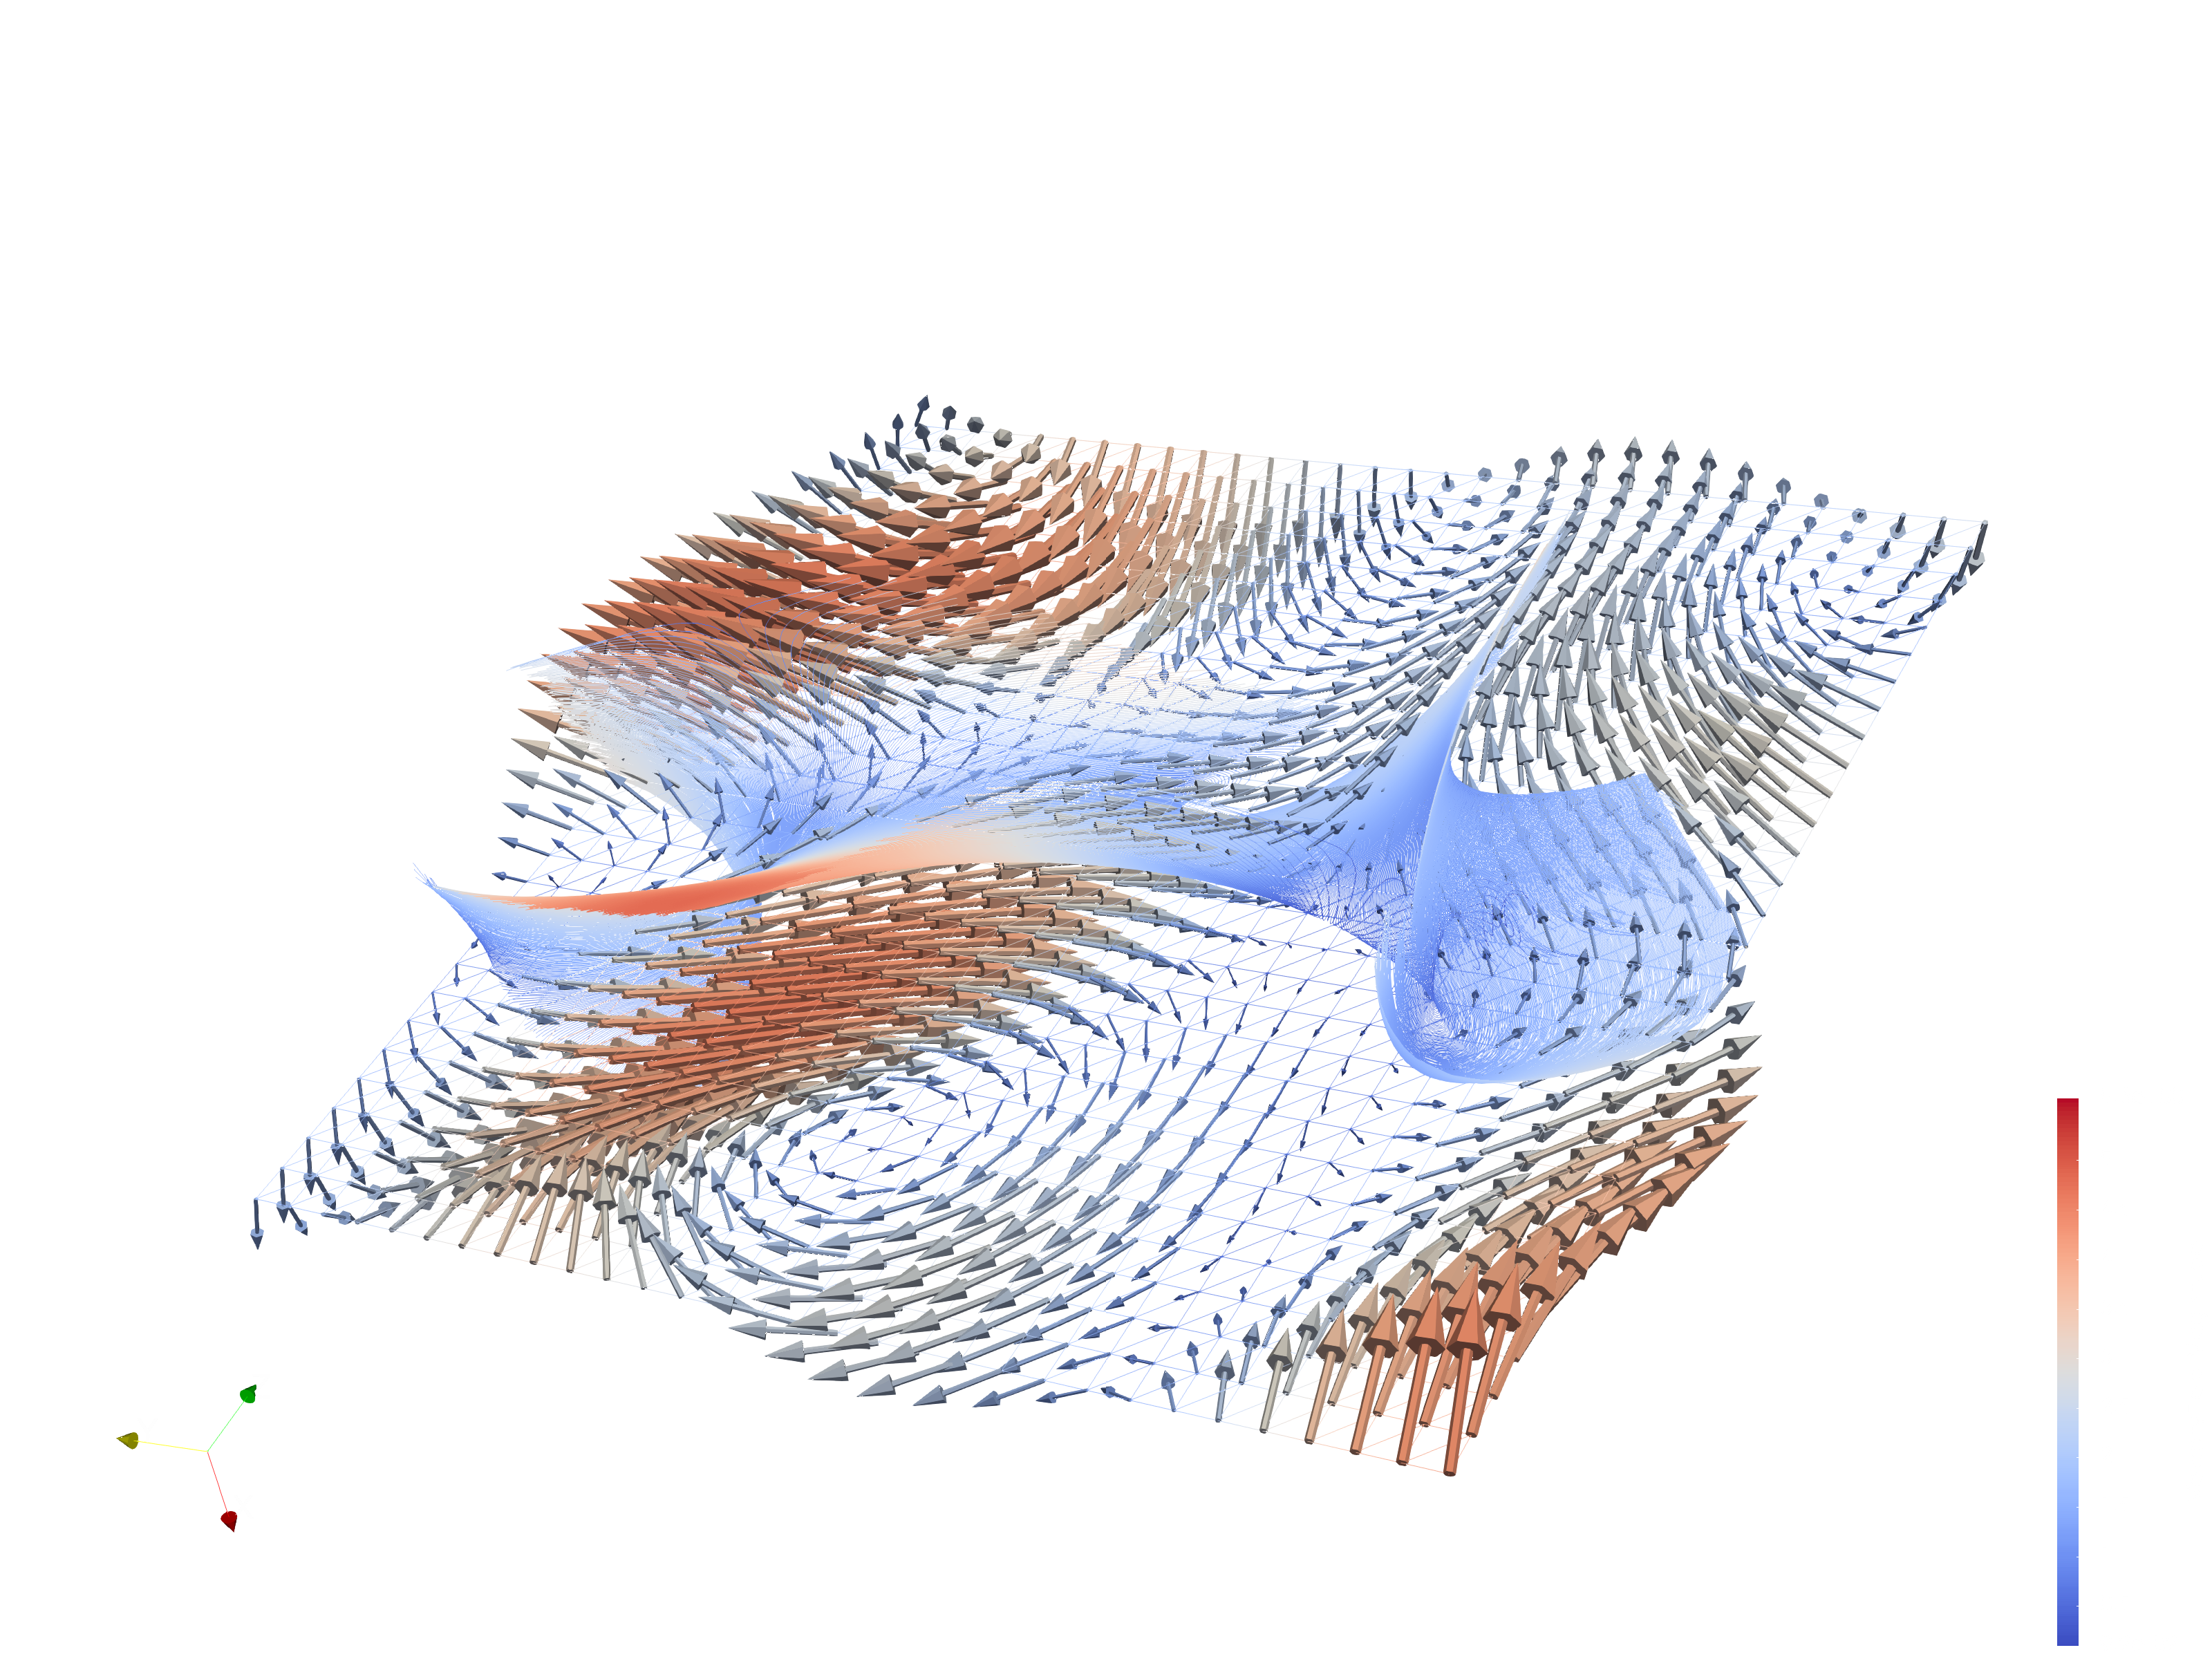
\includegraphics[width=0.4\linewidth]{images/spectral/spectral_n32_l10_f1000_k0pi3/spectral_x_normal_velocity_field_angle_trace.png}} \\
        \hfill
        \subcaptionbox[List-of-Figures entry]{плоскость $xy$, $z = 0$\label{img:spectral_slice_veloctiy_field_x_znormal_angle}} 
        {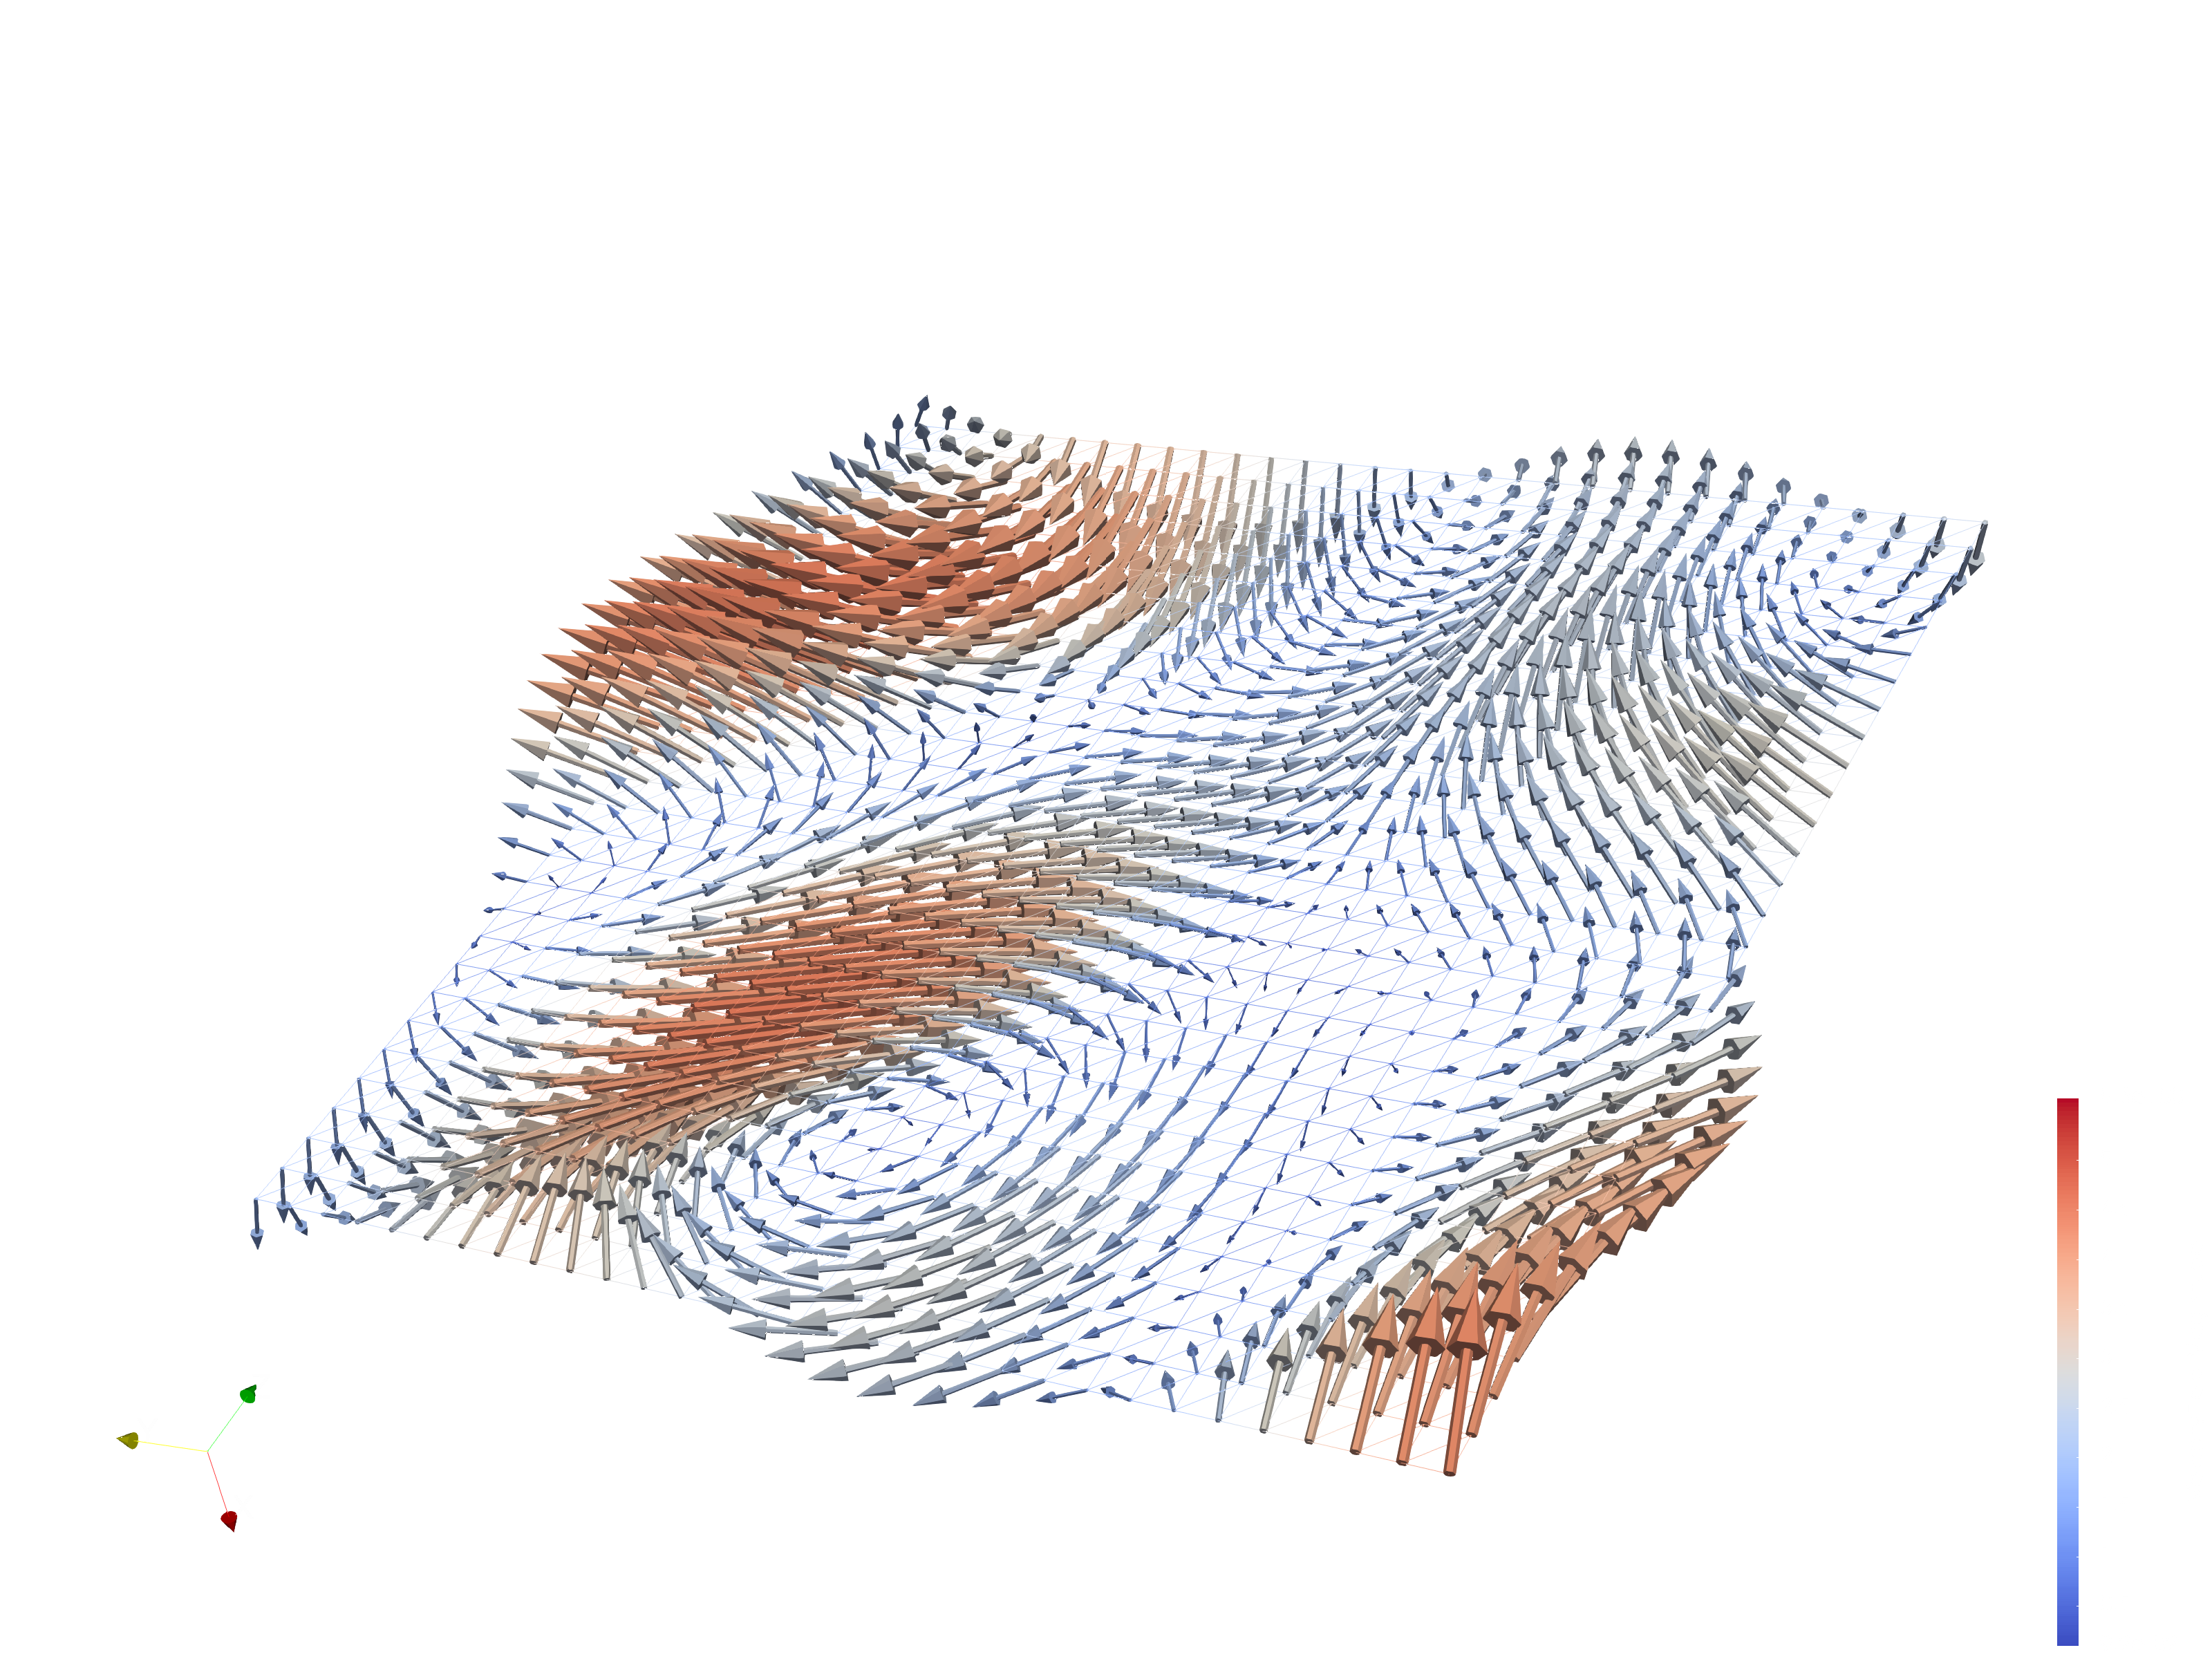
\includegraphics[width=0.4\linewidth]{images/spectral/spectral_n32_l10_f1000_k0pi3/spectral_x_normal_velocity_field_angle.png}}%
        \hfill       
        \subcaptionbox{плоскость $xy$, $z = 0$\label{img:spectral_slice_veloctiy_field_x_znormal_no_angle}} 
        {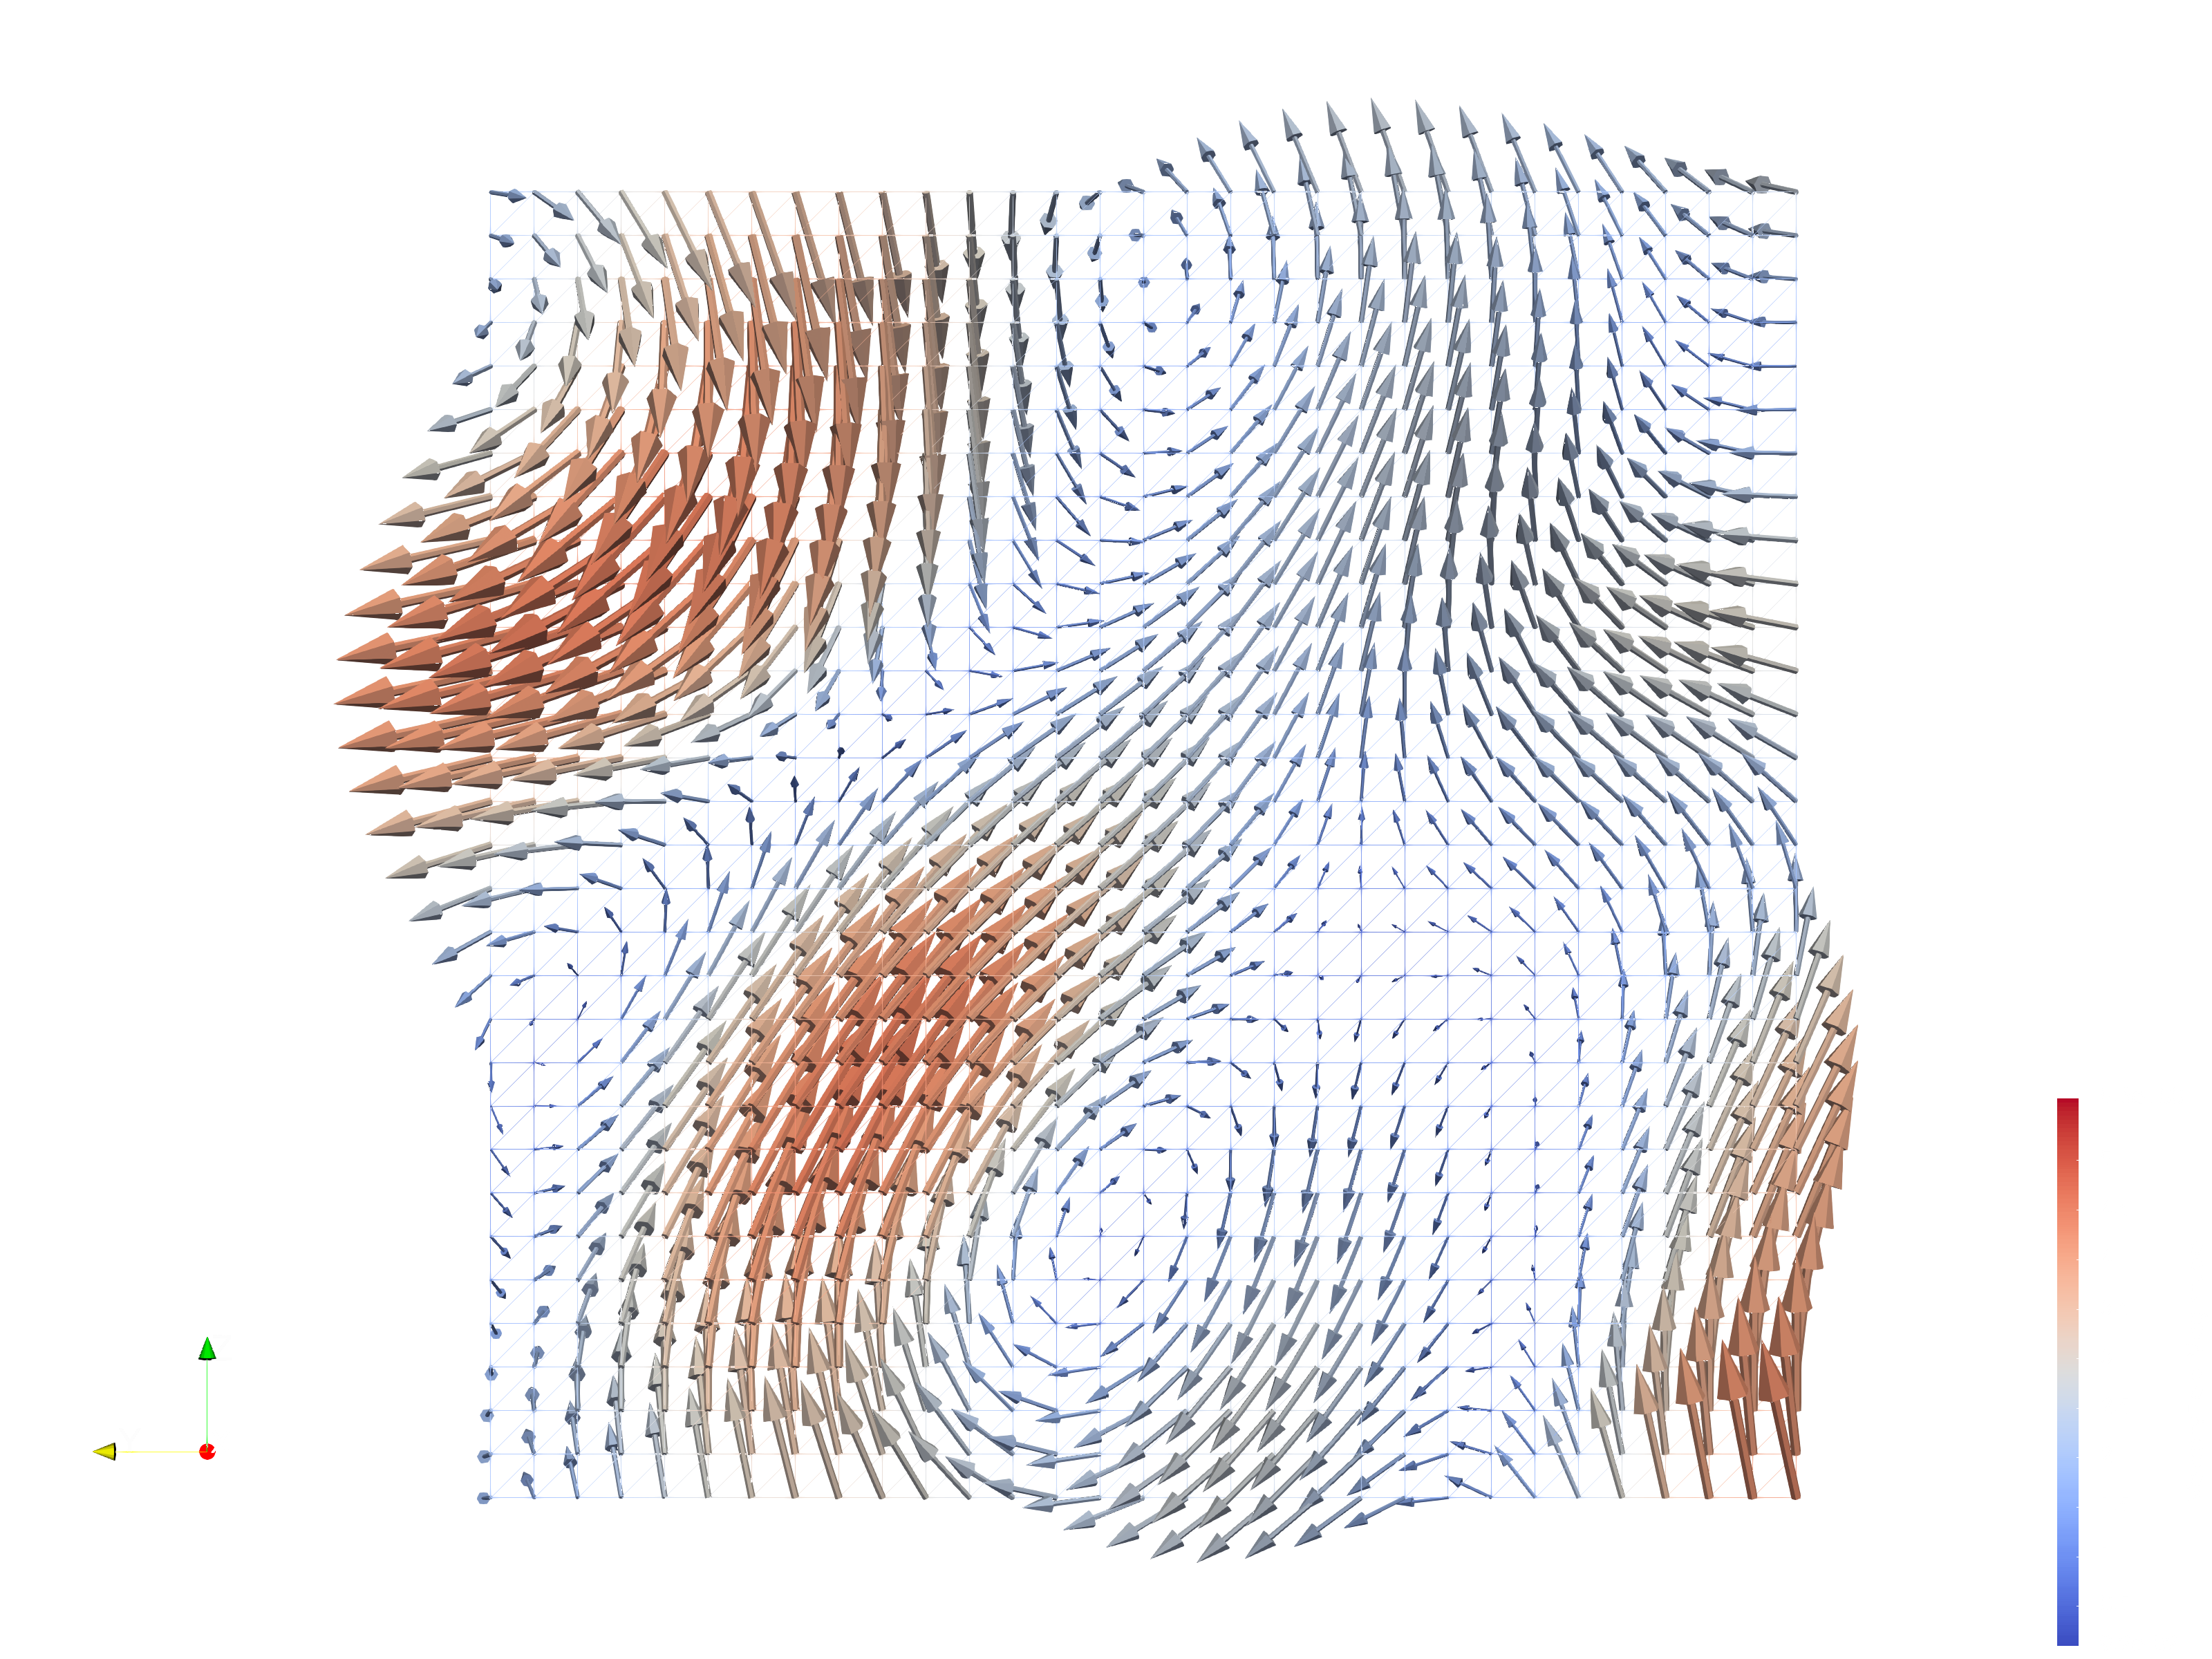
\includegraphics[width=0.4\linewidth]{images/spectral/spectral_n32_l10_f1000_k0pi3/spectral_x_normal_velocity_field.png}}
        \hfill
    }
    
    \onehalfspacing{Поле на картинке б представлено с линиями тока, расчитанными вдоль оси $y$}
    \caption{Поле флуктуаций сгенерированных трёхмерным стохастическим методом, цветом обозначена амплитуда флуктуаций}
    \label{img:velocity_fluctuation_field_for_spectral_1}  
\end{figure}

В отличие от стохастического метода, данный метод имеет явную зависимость вектора флуктуации от времени. Как говорилось выше, в данном случае распределение определяется сгенерированными частотами $\omega_0$. Мы можем выделить некоторый характерный период как $T = \frac{2 \pi}{\omega_0} = \frac{2 \pi}{k_0 v_0}$. Обычно при рассмотрении временных процессов берут период времени $100 T$, где $T = T_0$ -- характерный для задачи период (масштаб) времени. Шаг по времени выберем как $\Delta t = \frac{100 T_0}{N_{samples}}$ -- так мы можем трактовать поля сгенерированные во времени как одну реализацию поля флуктуаций. Ниже представлены сгенерированные поля для некоторых моментов времени. В общем случае, при данном шаге по времени наблюдается как плавный переход от одного поля к другому, так и достаточно резкий. Можно варьировать этот параметр путём задания среднеквадратичного отклонения для генерируемых частот -- $\omega_0$. Так для больших частот проявляется более частая смена ориентации векторов в пространстве.

%
%
% ТУТ КАРТИНКИ СГЕНЕРИРОВАННЫХ ПОЛЕЙ ВО ВРЕМЕНИ
%
%

На полученных реализациях мы можем оценить ковариационную функцию и последующими преобразованиями получить из неё и энергетический спектр. Ниже представлен рассчитанный на полученных реализациях тензор ковариаций относительно центра куба, совпадающего с началом координат, для различных направлений: по диагонали куба, по оси $x$, по оси $y$, по оси $z$, проходящие через начало координат. Различными цветами представлены компоненты тензора ковариаций. 

В случае однородной и изотропной турбулентности и несжимаемой жидкости есть возможность получить аналитическое выражение как для тензора ковариаций от функции энергетического спектра, так и для тензора спектра скорости от функции энергетического спектра \cite{Kraichnan70, pope2000turbulent}.

\begin{equation}
    \label{eq:part3_1}
    \left< \vec u (\vec x, t') \vec u (\vec x + \vec r, t) \right> = 2 D(t - t') \int_{0}^{\infty} E(k) \frac{\sin{(k r)}}{k r} dk 
\end{equation}

\begin{equation}
    \label{eq:part3_2}
    \Phi_{ij}(\vec k) = \frac{E(k)}{4 \pi k^2} \left( \delta_{ij} - \frac{k_i k_j}{k^2} \right)
\end{equation}

\noindent
здесь $k$ -- модуль волнового вектора, $k_i$ -- компонента волнового вектора.
Для обоих рассматриваемых методов генерация осуществляется в рамках однородной и изотропной турбулентности для несжимаемой жидкости, тем самым мы можем сравнить не только, например, спектральные характеристики, но и также провести сравнение других характеристик, таких как тензор ковариаций и тензора скоростей.

Рассмотрим полученные ковариационные функции на рассчитанные на 10000 реализаций поля флуктуаций с параметрами описанными выше.

\begin{figure}[!h]
    \center{
        \hfill
        \noindent \subcaptionbox[List-of-Figures entry]{диагональ куба\label{img:spectral_covariance_diagonal}} 
        {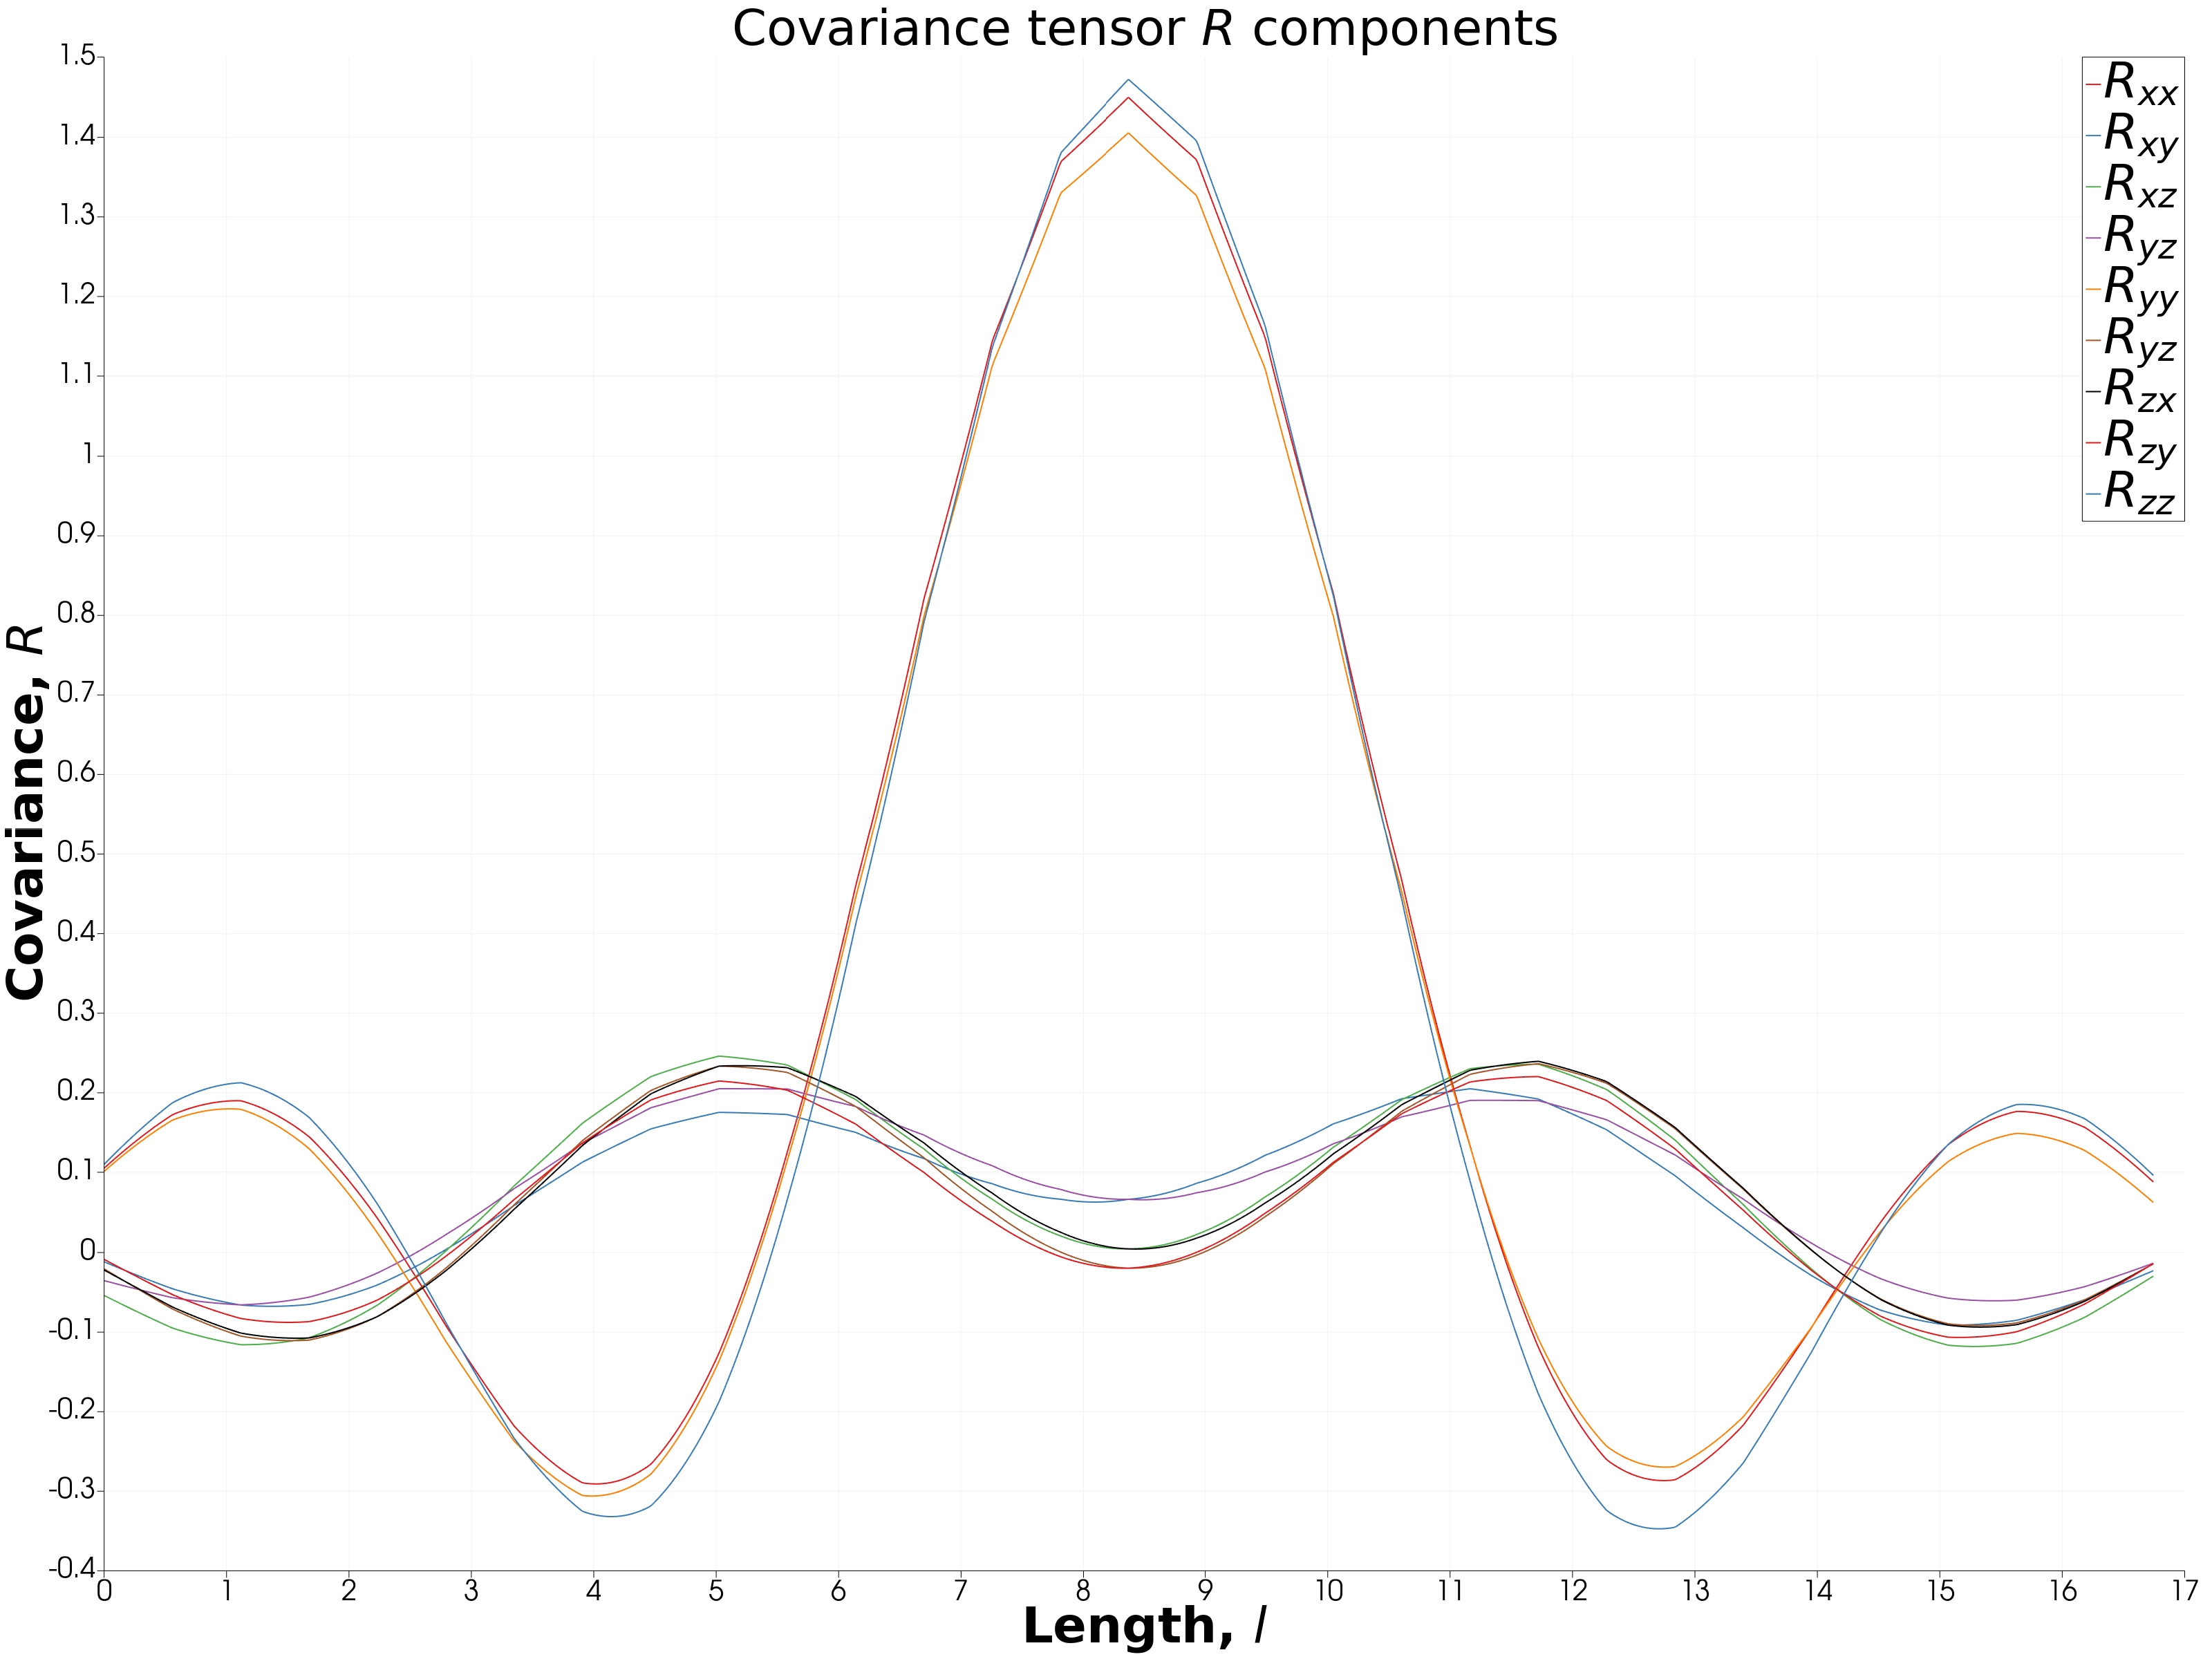
\includegraphics[width=0.4\linewidth]{images/spectral/spectral_n32_l10_f1000_k0pi3/covariance_function_diagonal.png}}%
        \hfill       
        \subcaptionbox{$x$\label{img:spectral_covariance_x}} 
        {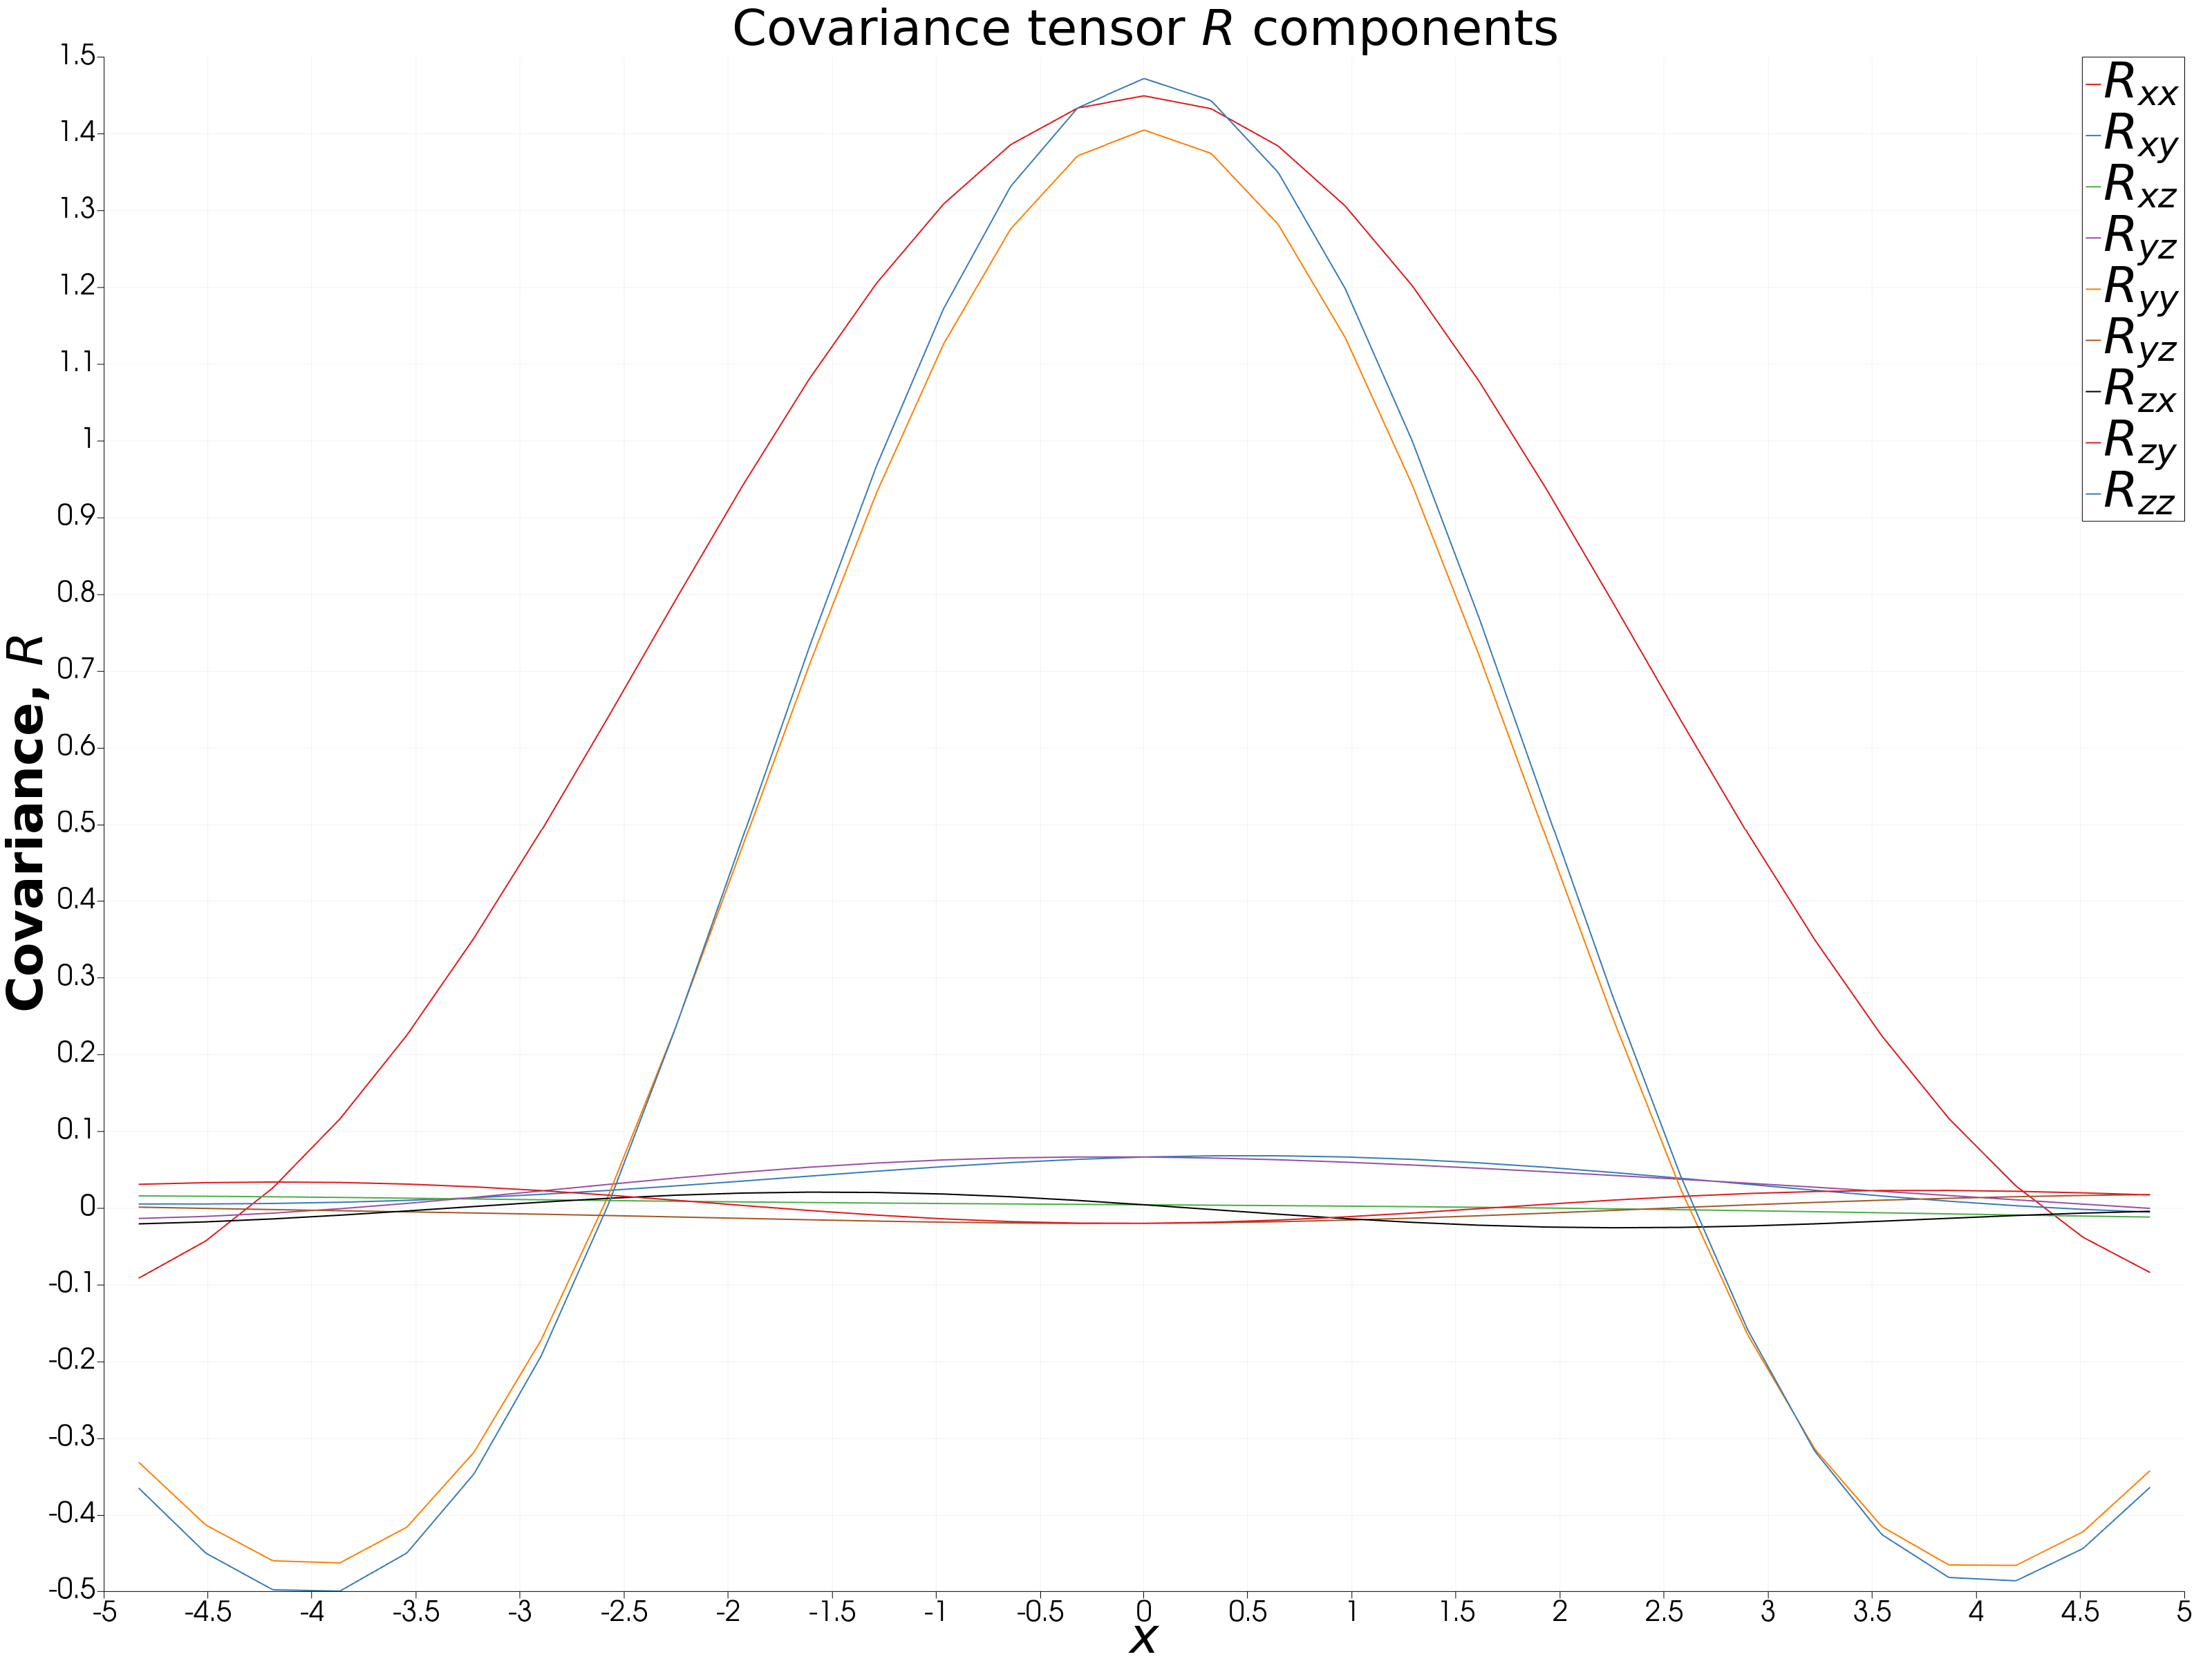
\includegraphics[width=0.4\linewidth]{images/spectral/spectral_n32_l10_f1000_k0pi3/covariance_function_x.png}} \\
        \hfill
        \subcaptionbox[List-of-Figures entry]{$y$\label{img:spectral_covariance_y}} 
        {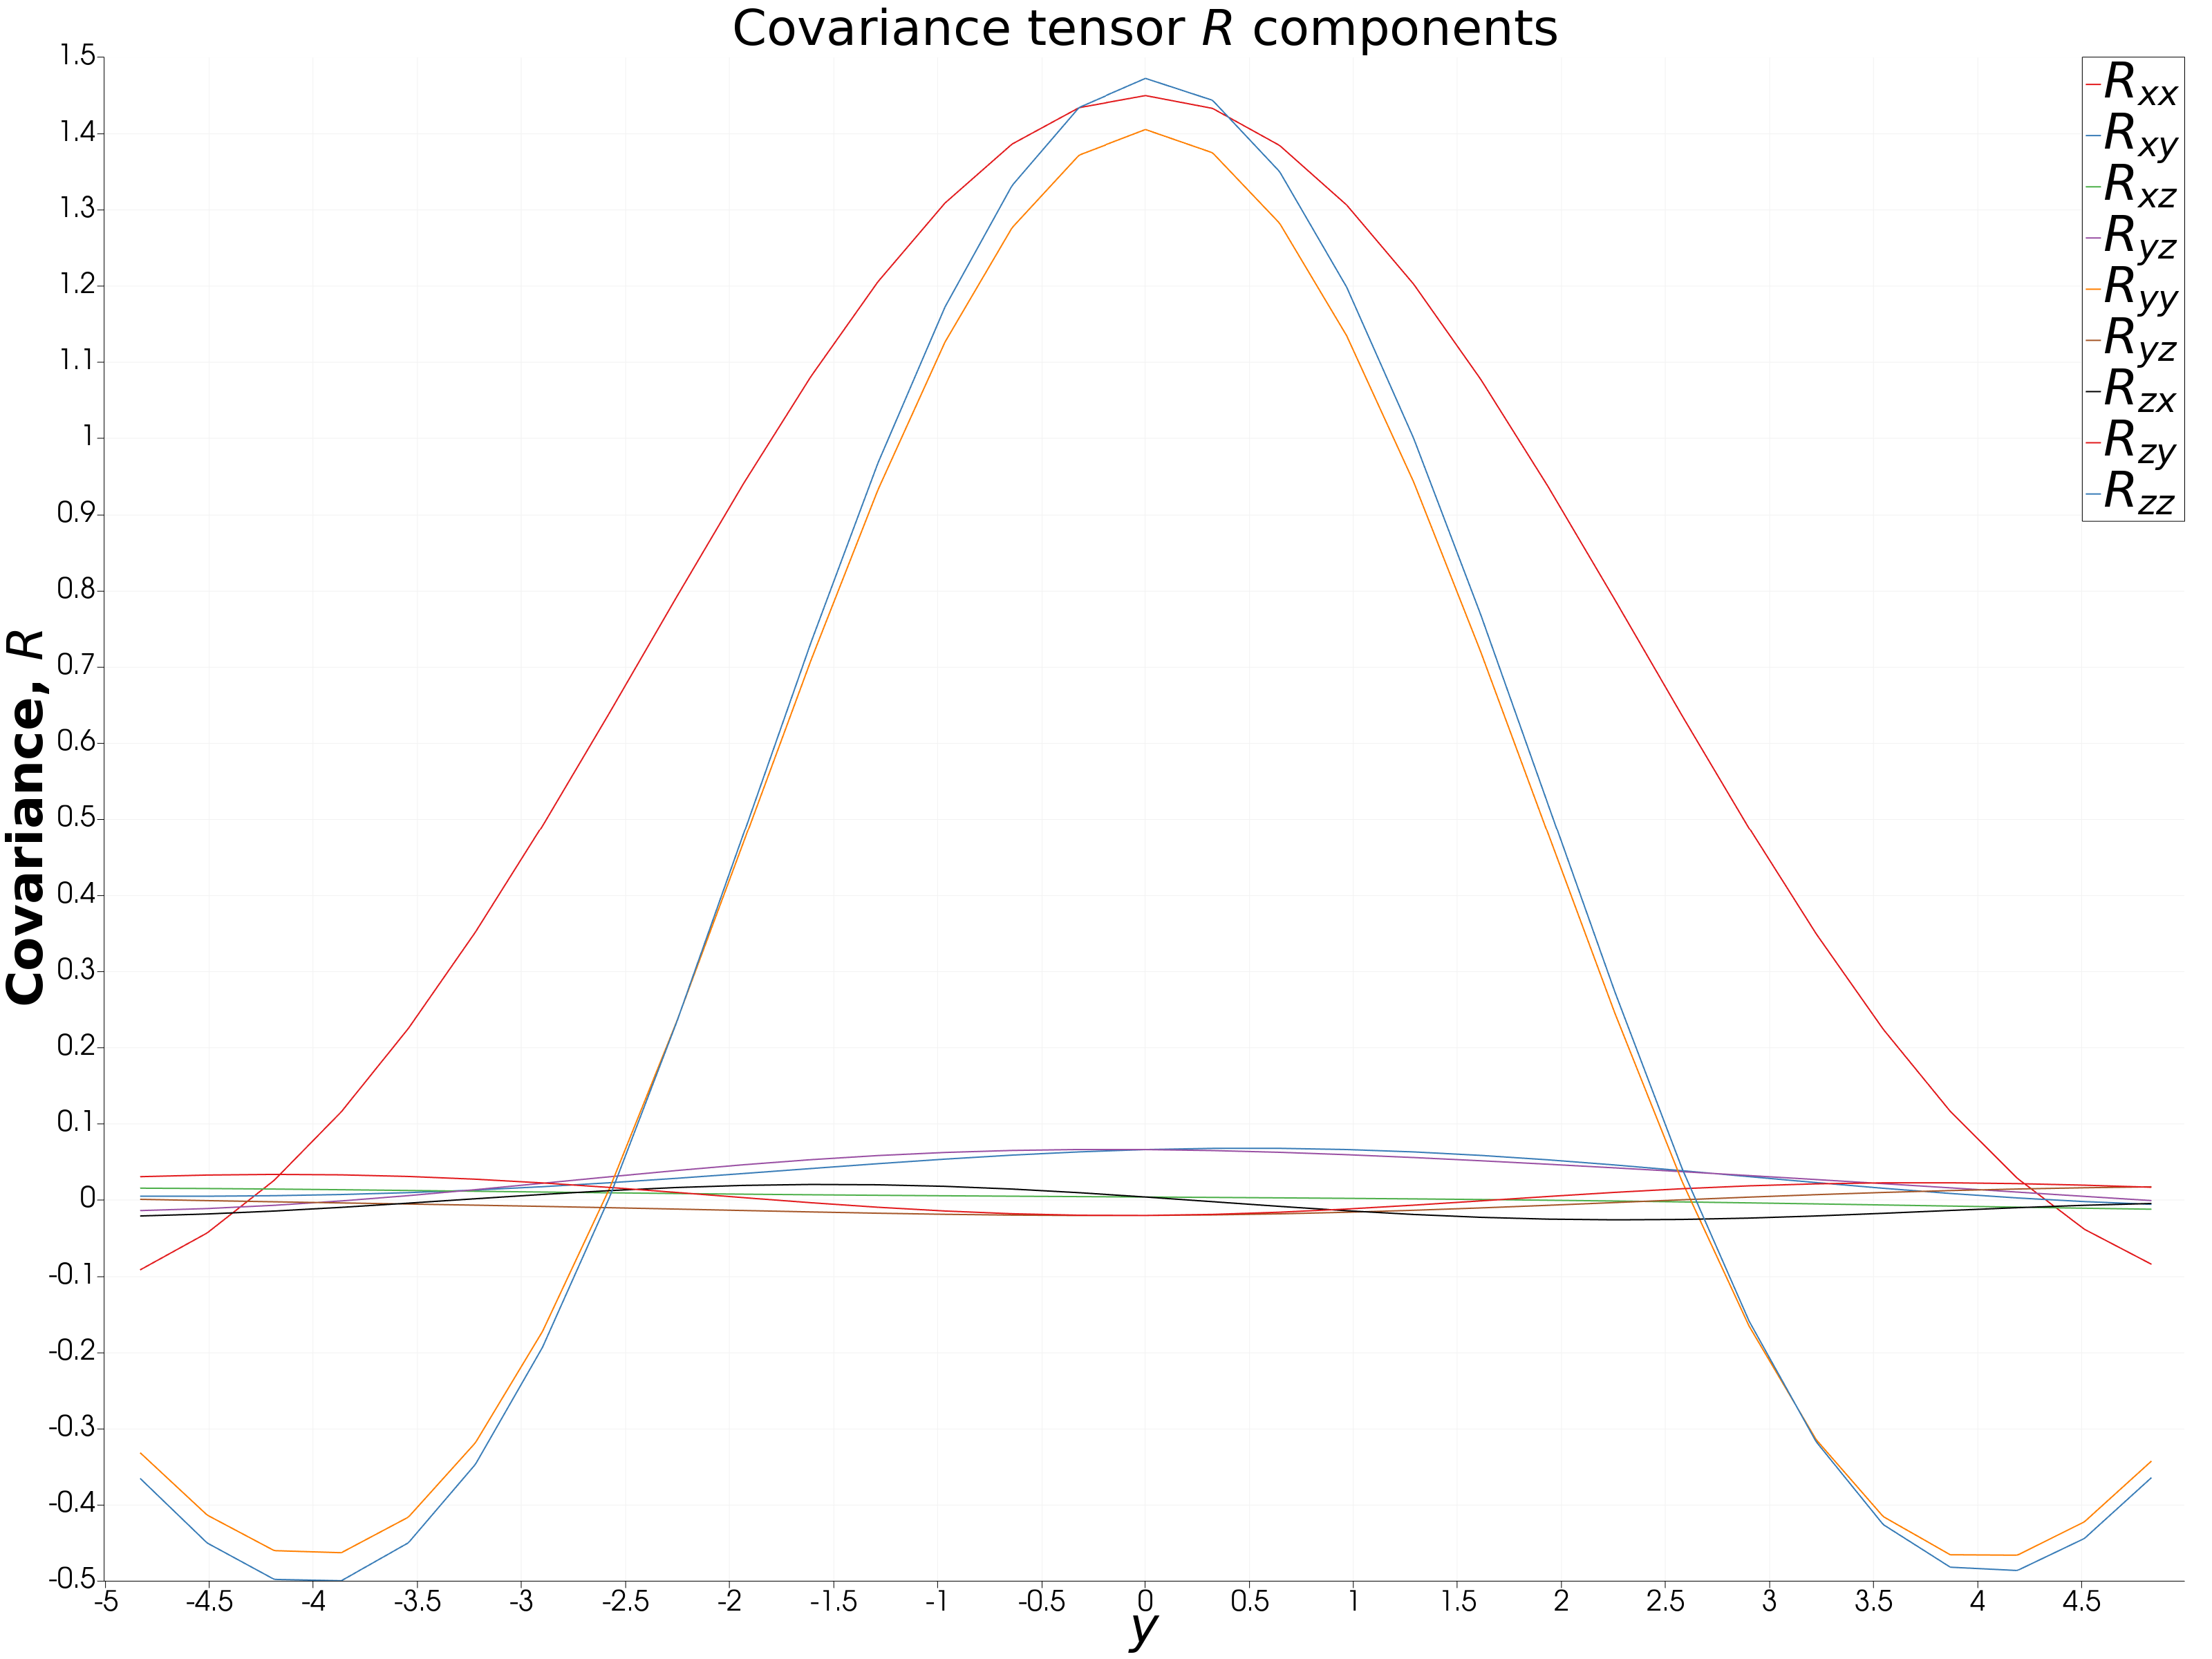
\includegraphics[width=0.4\linewidth]{images/spectral/spectral_n32_l10_f1000_k0pi3/covariance_function_y.png}}%
        \hfill       
        \subcaptionbox{$z$\label{img:spectral_covariance_z}} 
        {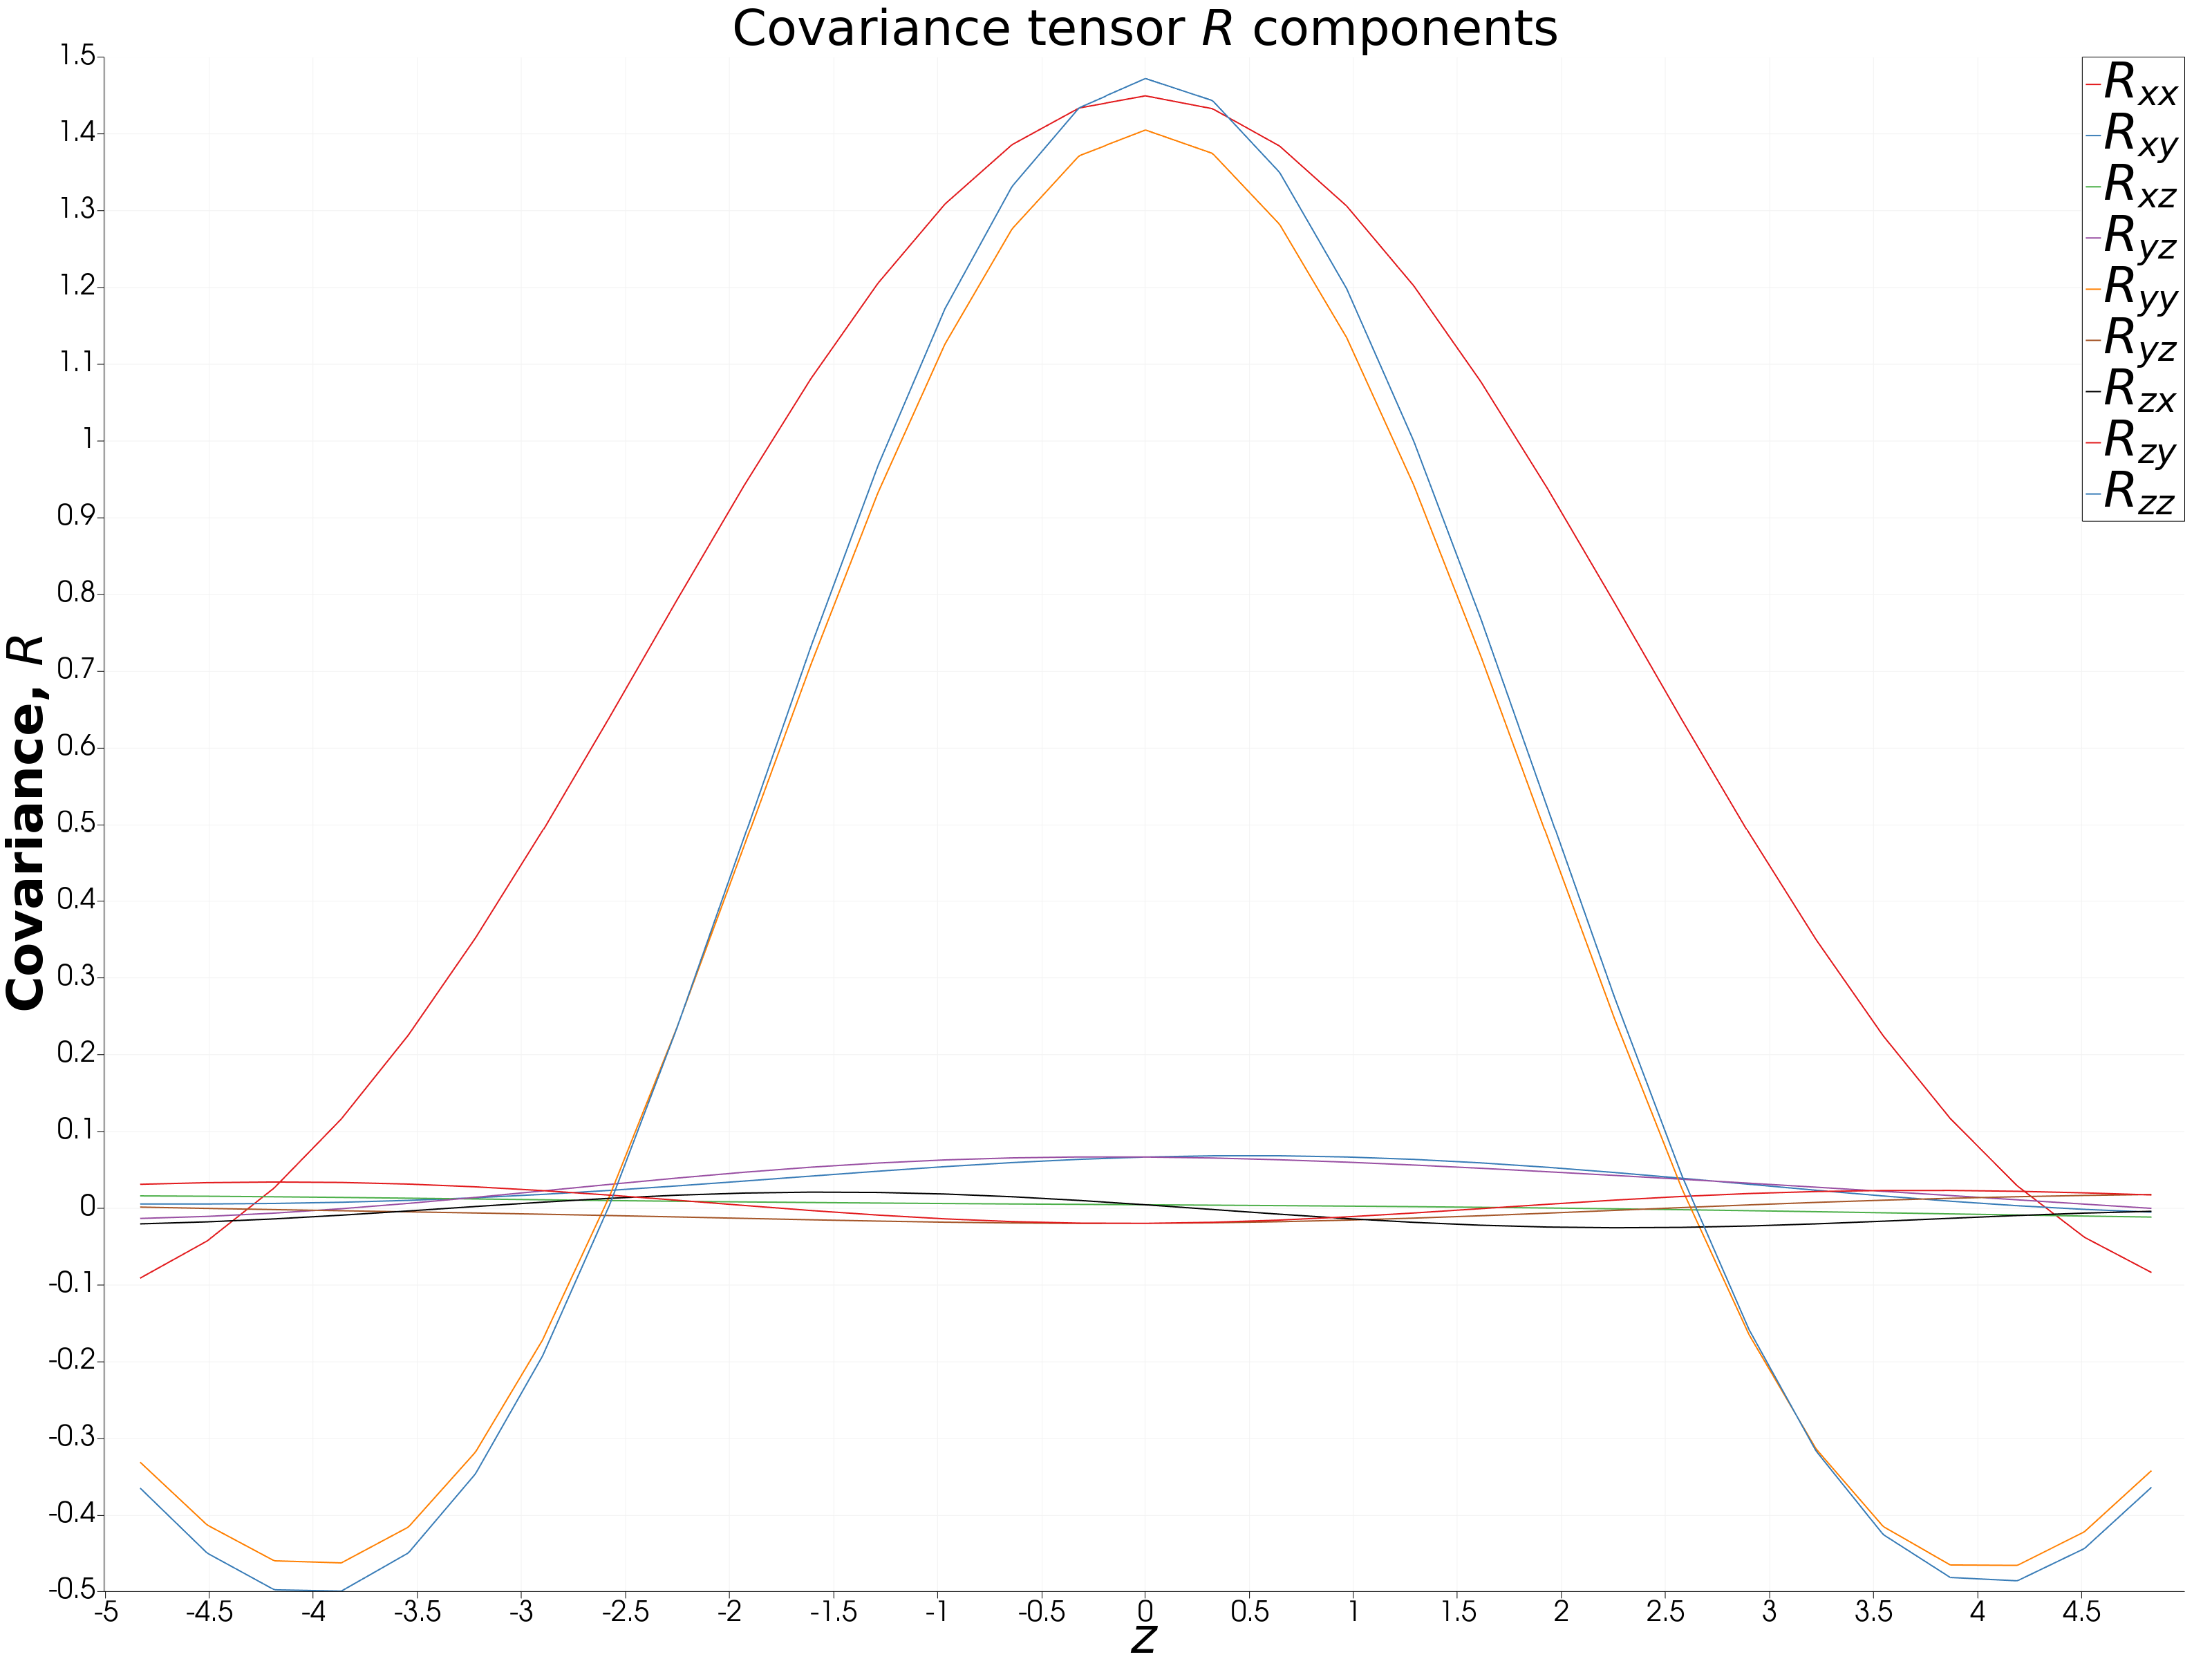
\includegraphics[width=0.4\linewidth]{images/spectral/spectral_n32_l10_f1000_k0pi3/covariance_function_z.png}}
        \hfill
    }
    
    \onehalfspacing{Поле на картинке б представлено с линиями тока, расчитанными вдоль оси $y$}
    \caption{Поле флуктуаций сгенерированных трёхмерным стохастическим методом, цветом обозначена амплитуда флуктуаций}
    \label{img:velocity_fluctuation_field_for_spectral_2}  
\end{figure}

По аналогии с методом Хуанга, мы можем генерировать поле флуктуаций как суперпозицию полей построенных для различных волновых чисел, а соответственно и для различных значений энергии. В этом случае $\vec u = \sum_{k_{i}} \vec u_i$, где $\vec u_i$ -- флуктуация, сгенерированная для определённого волнового числа $k_i$. Как и ранее, остается сложностью оценить наперед среднеквадратичное отклонение для проведения нормировки высоты спектральных линий для аппроксимации целевого спектра. Но мы можем сделать следующее, энергетический спектр турбулентности связан с кинетической энергии турбулентности $\kappa = \int_{0}^{\infty} E(k) dk$, отсюда мы можем взять, что $\kappa(k_m) = E(k_m) \Delta k$, и получаемую величину флуктуации скорости нормировать на значение $\sqrt{E(k_m) \Delta k}$. 

Одним из других подходов состоит в нормировке не результирующего значения флуктуации, а в нормировке амплитуд мод Фурье. В отличие от нормировки результирующего вектора флуктуаций, в данном подходе на выходе также получаются различные амплитуды флуктуаций с сохранением зависимости от амплитуды спектра. Для ускорения процесса генерации можно использовать разложение лишь по одной тригонометрической функции, например лишь по функции косинуса. В итоге можно использовать разложение представленное в виде:

\begin{equation}
    \label{eq:part3_3}
    \vec v(\vec r, t) = \alpha \sum_{n = 1}^{N} \vec p_n \cos( \vec k_n \cdot \vec r + \omega_n \cdot t + \psi)  
\end{equation}

\noindent 
здесь, $\vec p_n$ -- амплитуды мод Фурье, генерируемые изначально на единичной сфере так, чтобы $\vec p_n \cdot \vec k_n = 0$, для сохранения удовлетворению уравнению неразрывности, с последующим привидением к длине равной $\sqrt{E(k_n)\Delta k}$, $\psi_n$ - случайная фаза, добавленная для компенсации исключения нечетных мод, генерируемая например из равномерного распределения в пределах $-\pi$ до $\pi$, $\alpha$ -- нормировочный коэффициент, который можно взять, например $\sqrt{\frac{2}{N}}$, как в методе Смирнова(\ref{sect2_2}), либо провести нормировки на кинетическую энергию по аналогии с методом Шура (\ref{sect2_4}): $\sqrt{\frac{1}{\sum_{n=1}^{N} E(k_n) \Delta k_n}}$. По построению амплитуд Фурье лучше всего использовать последнее определение для нормировочного коэффициента $\alpha = \sqrt{\frac{\beta}{\sum_{n=1}^{N} E(k_n) \Delta k_n}}$, после проведения тестовых расчётов мы получили что оптимальным значение для коэффициента $\beta \approx 2$. Связано это с тем, чтобы в формуле \eqref{eq:kriging_equation15} компенсировать коэффициент $\frac{1}{2}$

Для проведения статистического анализа предлагаемой модификации спектрального метода использовалось 5000 реализаций со следующими параметрами:
\begin{enumerate}
    \item Длина куба: $l = 10$, центр совпадает с началом координат;
    \item Число разбиений по каждой из сторон куба: $n = 51$;
    \item Число взятых мод Фурьe: $N = 1000$;
    \item Интервал волновых чисел: $(k_{min} = 0.01, k_{max} = 10$, число разбиений для дискретизации спектра совпадает с числом мод Фурье;
\end{enumerate}

Наименьшее волновое число для рассматриваемой сетке: $k_{min} = \frac{2 \pi}{l} \approx 0.6283$ -- максимальное волновое число: $k_{max} = \frac{\pi}{\dfrac{l}{n}} \approx 16.022$. Приведём сравнение спектра рассчитанного для приведённого выше числа сгенерированных реализаций с входным спектром.

\begin{figure}[ht] 
    \center
    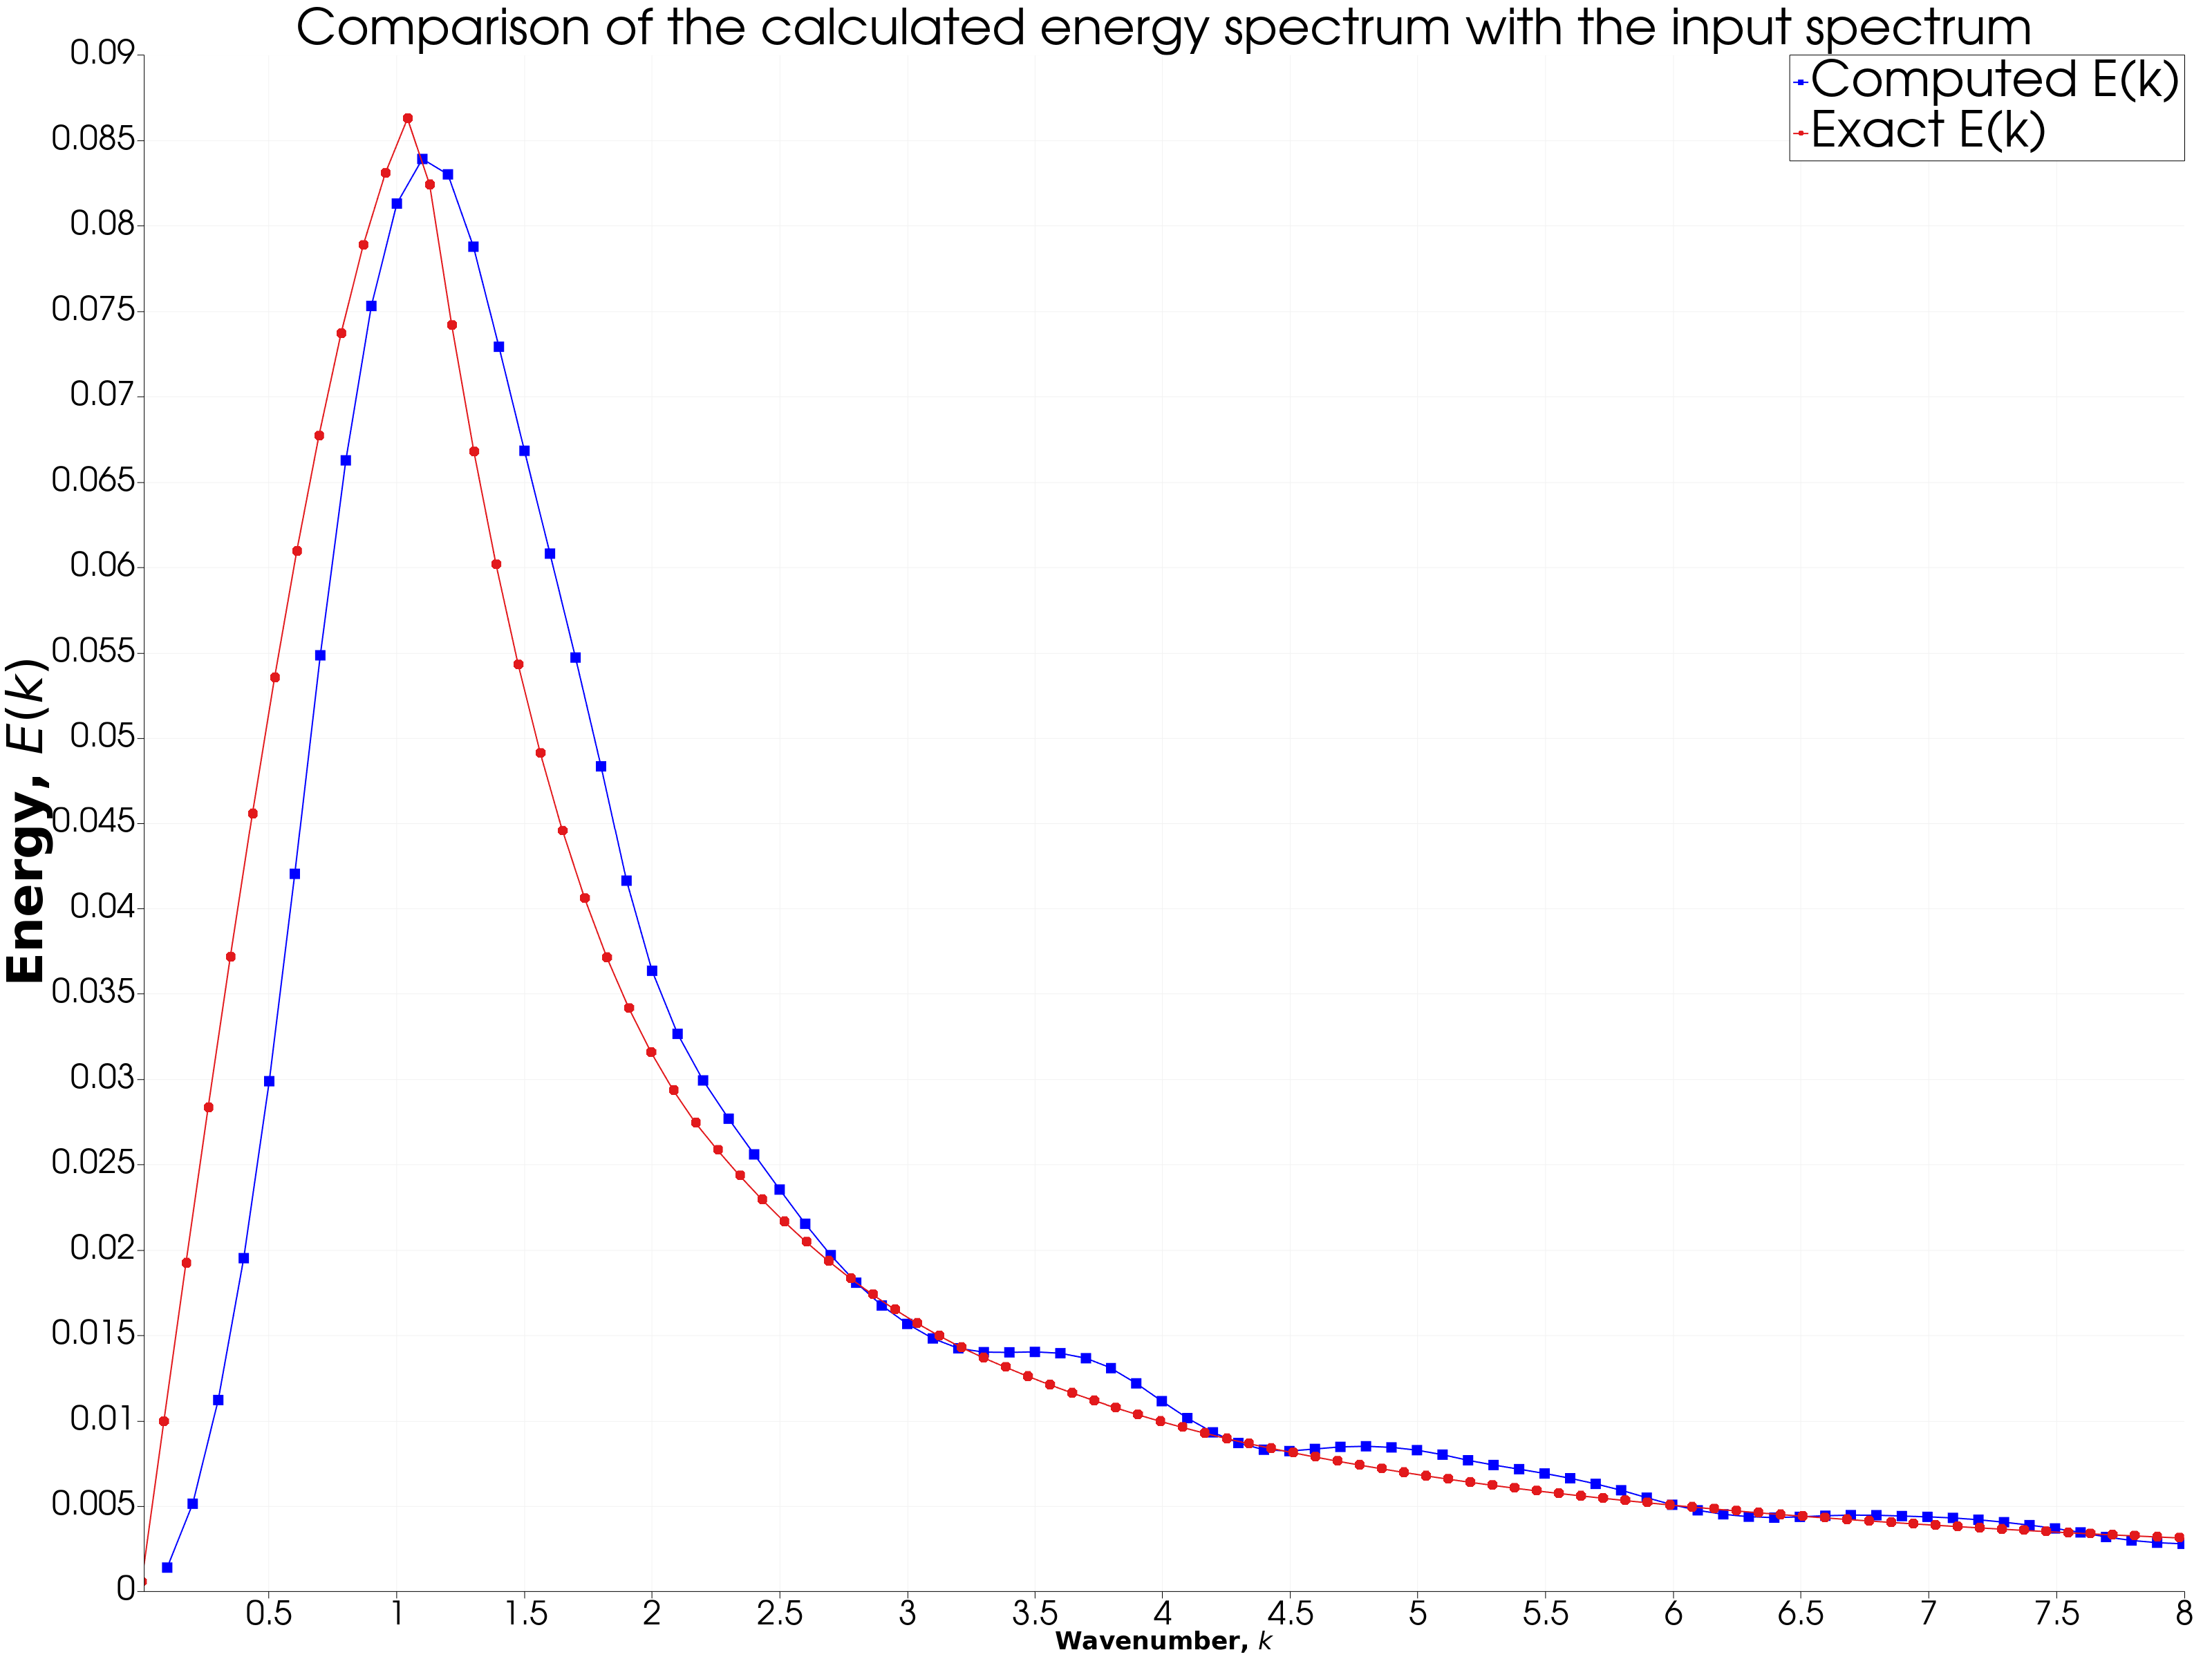
\includegraphics [width=0.8\linewidth] {images/spectral/spectra_l10_k10_f1000_n51.png}
    \caption{Сравнение энергетического спектра для предлагаемой модиификации спектрального метода с задаваемым.} 
    \label{img:spectral_desam_spectra_comarison}  
\end{figure}

\begin{figure}[ht] 
    \center
    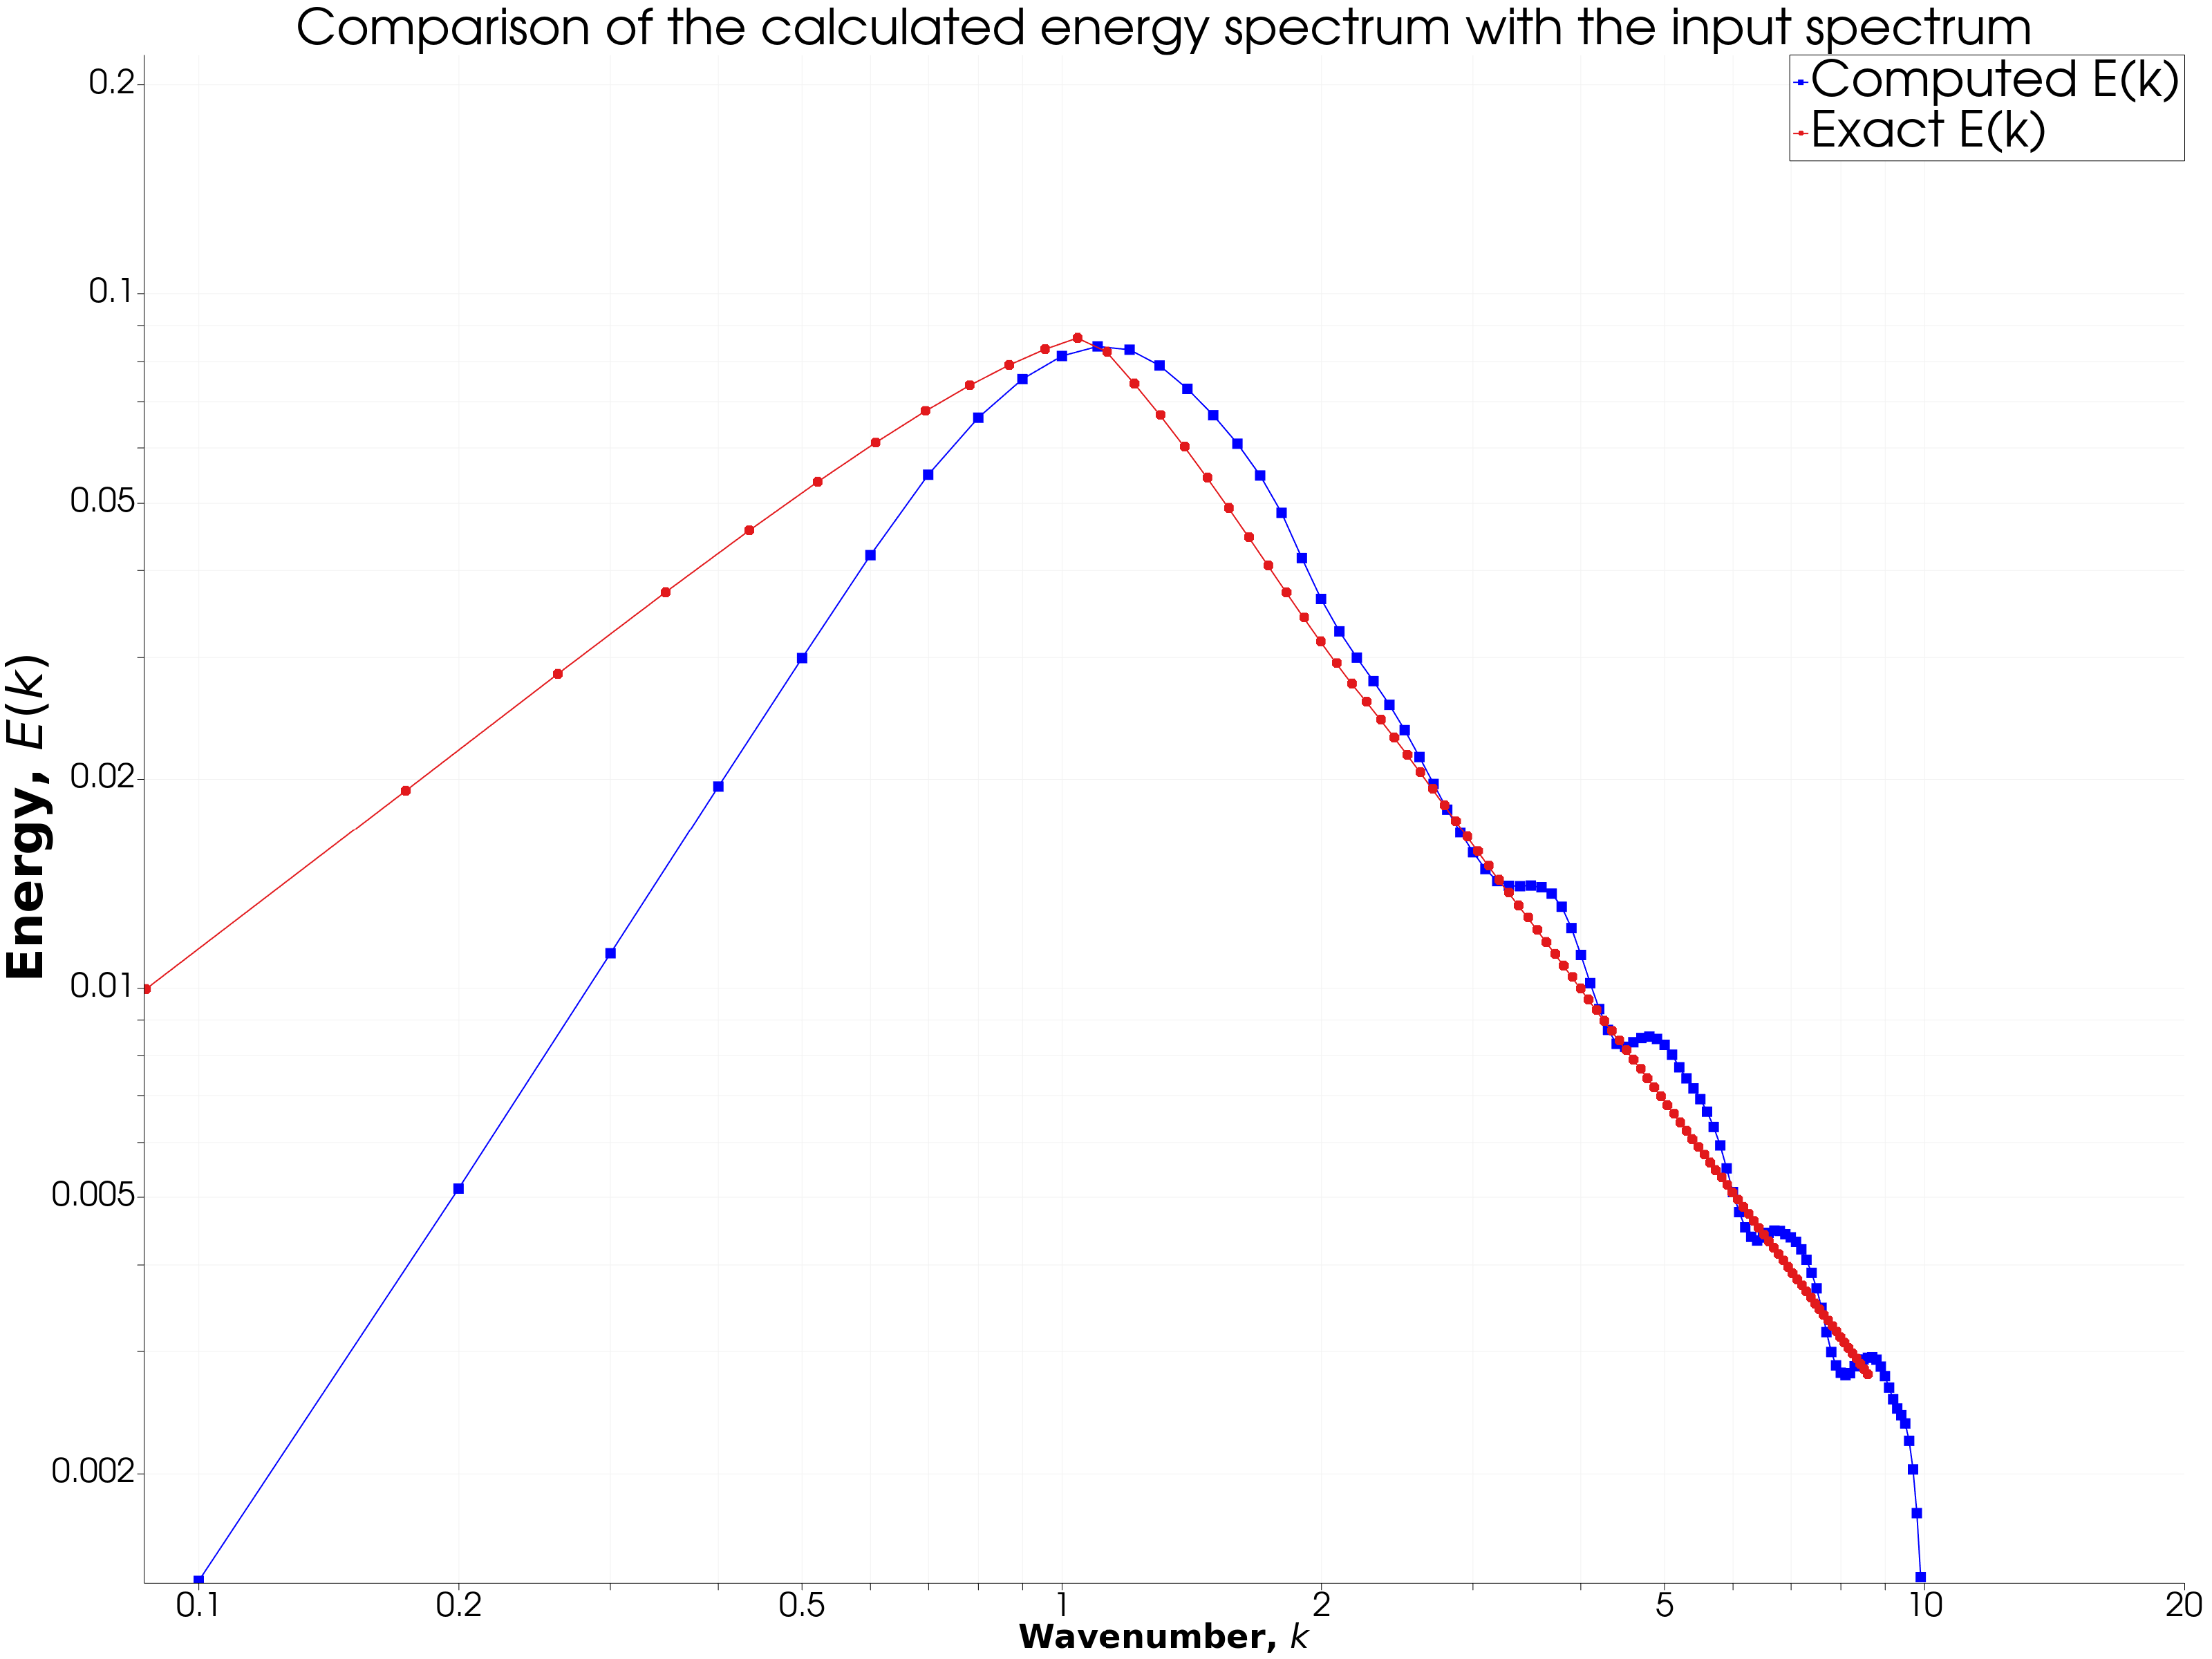
\includegraphics [width=0.8\linewidth] {images/spectral/spectra_l10_k10_f1000_n51_loglog.png}
    \caption{Сравнение энергетического спектра для предлагаемой модиификации спектрального метода с задаваемым в логарифмических координатах} 
    \label{img:spectral_desam_spectra_comarison}  
\end{figure}

Во первых заметим большую разницу для малых значений волнового числа, связанное с тем что минимальное волновое число меньше чем волновое число для рассматриваемой сетке, в своб очередь в диапазоне начиная с минимального для сетки волнового числа наблюдается хорошее совпадение с целевым спектром, особенно в инерционном интервале, с хорошо известным законом $-\dfrac{5}{3}$.
  
\begin{figure}[ht] 
    \center
    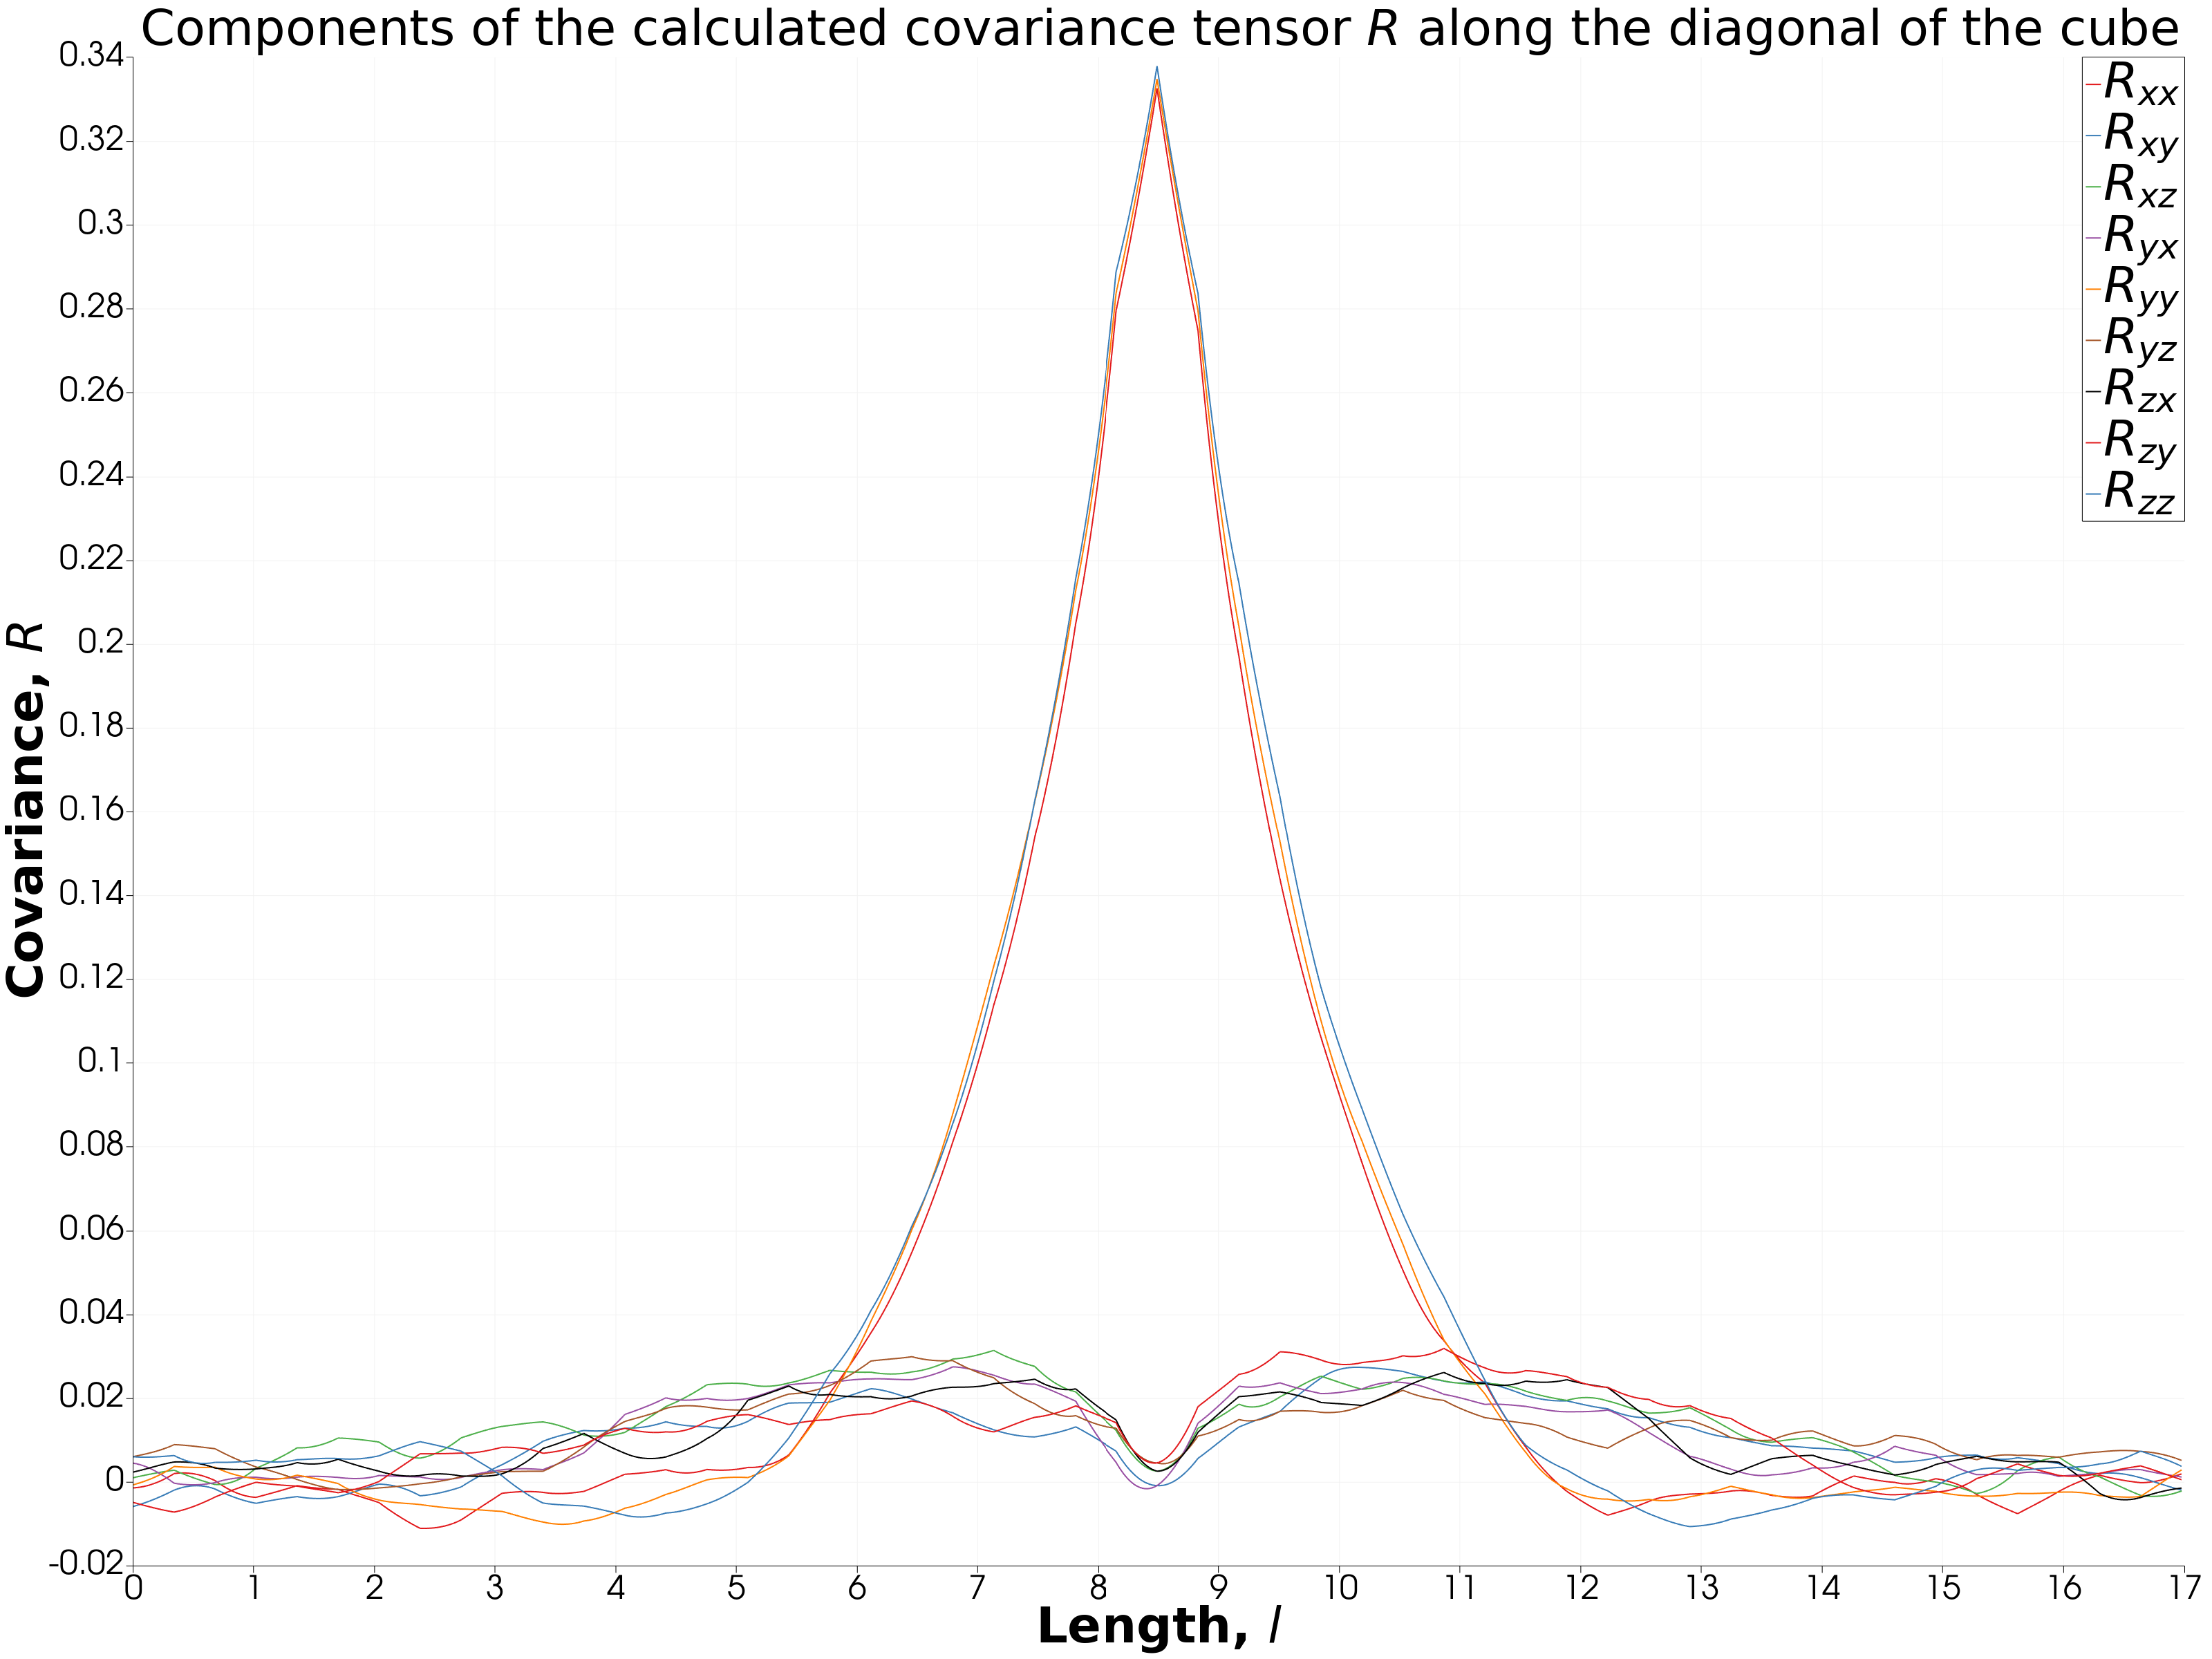
\includegraphics [width=0.8\linewidth] {images/spectral/covariance_function_tensor.png}
    \caption{Компоненты тензора ковариаций дволь диагонали вычислительной области} 
    \label{img:spectral_desam_covariance_comarison}  
\end{figure}

Сразу можно заметить, что по сравнению с генерацией на одной частоте, а именно методом Крайшнана, амплитуда ковариаций уменьшая бустрее с ростом расстояния от центра расчёта ковариации. Также уменьшилось расстояние на котором сохраняется пространственная ковариация двух величин, как было показано ранее, функция ковариации при генерации одной амплитуды сохраняет ковариацию на больших расстояниях, и имеет форму модулированной волны, в рассматриваемом сейчас случае, при достижении амплитуды ковариации при дальнейшем увеличении расстояния скоррелированость величин остаяется близи 0.

Приведём несколько сгенрированных полей флуктуаций с использованием предложенного метода. На рисунках ниже представлено по 3 плоскости с отображением направлений флуктуаций, для того чтобы показаться изменение векторов не только в плоскости $yz$ по нормали к оси $x$, центр поддомена совпадает с центром расчётной области.


\begin{figure}[ht] 
    \center
    \includegraphics [width=0.8\linewidth] {images/spectral/field_on_x_normal_yz_plane.png}
    \caption{Сгенерированное поле флуктуаций модифицированным методом, длины векторов пропорциональны длине векторов флуктуаций} 
    \label{img:spectral_result_field_no_angle}  
\end{figure}

\begin{figure}[ht] 
    \center
    \includegraphics [width=0.8\linewidth] {images/spectral/field_on_angle.png}
    \caption{Сгенерированное поле флуктуаций модифицированным методом, длины векторов пропорциональны длине векторов флуктуаций} 
    \label{img:spectral_result_field_on_angle}  
\end{figure}

На представленых рисунках хорошо видно вихревое движение во всех направлениях. За счёт пропорциональности длины векторов мы можем явно качественно разделить течение на зоны. 

Для сравнения методов по производительности использовалась сетка размерностью $n = 31$ и размером $l=10$. Для спектрального метода использовалось 1000 мод фурье с покрытием всего интервала волновых чисел, с такими параметрами достигается максимальная производительность не в угоду точности. Замер среднего времени генерации проводился на 1000 генераций. Полное время, потребовавшееся для генерации 1000 реализаций составило в среднем ~44 секунды, среднее время для генерации одной реализации поля скорости $\frac{44}{1000} \ approx 0.044$, принебрегая временем на операции записи результатов в файл.

% ---------- %
%  CHAPTER 4
% ---------- %
 
\chapter{Валидация стохастического метода генерации синтетической турбулентности} \label{chapt5}
Перед использованием метода стохастического моделирования необходимо оценить влияние параметров данного метода. В отличие от спектральных методов, смысл проверки параметров можно назвать в данном случае другим. От таких параметров как допуск по величине ковариации и количеству собственных значений, зависит не столько конечный результат, сколько требуемая вычислительная мощность. На примере одномерного моделирования рассмотрим влияние параметров числа находимых собственных значений и выбираемым значениям амплитуд ковариации. Число собственных чисел входит в конечную формулу для генерации случайных чисел с заданной корреляцией, в силу того, что используется в итоге конечное число случайных чисел, необходимо проследить как влияет на решение их число. Также при нахождении собственных чисел появлялись отрицательные собственные числа, что является нежелательным эффектом. Связано это может быть с упомянутым в главе \ref{chapt2} свойством неотрицательной определённости матрицы ковариаций. Из этого не следует возможность в появлении отрицательных собственных чисел, но из-за машинного шума компоненты матрицы ковариации могут быть меньше 0, когда они равны в точности 0 и побудить появление отрицательных собственных чисел. Также необходимо учесть, что метод нахождения собственных чисел построен на итерационном процессе, в котором также может накапливаться ошибка.

При рассмотрении допуска по величине ковариаций можно достаточно сильно сэкономить на заполненности матрица ковариаций, тем самым увеличив, например разбиение по сетке, либо увеличив хранимое число собственных чисел. Но это также влияет на коррелированность пар значений при случаях когда ковариация между ними равна 0. Также есть другая цена у допуска, больше значений матрицы ковариаций нулевые, хоть они и не хранятся в разреженной матрице, что как отмечалось выше, может спровоцировать появление отрицательных собственных чисел. В целом, можно использовать допуск одновременно исключая отрицательные собственные числа.

Как говорилось выше, для оценки влияния рассматриваемых параметров нужно было провести несколько вычислительных экспериментов. Число собственных чисел варьировалось от 100 до 600 с шагом 50, допуск по амплитудам ковариации варьировался от 0\% до 5\% с шагов в 1\%. Критерием удовлетворения заданным параметрам являться близость ковариационной функции построенного поля к задаваемой. Задаваемая ковариационная функция является по определению Фурье образом от функции турбулентного спектра, задаваемого аналитически.

Рассмотрим сравнение между полученными данными для всех случаев в срезах по осям $x, y, z$ (линия проходит через центр куба, совпадающий с началом координат) и диагонали между точками $\{-5, -5, -5\}$ и $\{5, 5, 5\}$ внутри куба со стороной равной 10, и числом разбиений 21 как для пространства Фурье и ковариационной функции, так и для разбиения реального пространства. Пространственная ковариация рассчиталась с использованием набора из 1000 генераций для одного набора собственных значений. Все рассматриваемые сечения проходят через центр, так как вид ковариационной функции близок к виду Гауссовой кривой либо кривой Лоренца с пиками в центре координат.

Как упоминалось ранее, в общем случае, метод может иметь в наборе собственных значений также отрицательные собственные числа. Их число зависит не только от собираемой матрицы ковариаций, но также и от параметров оборачивания этой матрицы. Без ограничений по числу итераций, а также с алгоритмом прохода по наибольшим собственных значениям среди 9200 собственных чисел (совпадает с размерностью матрицы ковариаций) около 200 являются отрицательными, это около $2\%$ от общего числа собственных чисел. Хоть это число и мало, необходимо оценить, сколько собственных чисел стоит брать для хорошего удовлетворения ковариационной функции. Число отрицательных собственных чисел также может расти/уменьшаться с изменением как параметров сетки, так и в целом параметров спектра, итерационного метода и самого базиса метода стохастического моделирования (например при использовании кокригинга). Хоть $2\%$ сама по себе достаточно малая величина, может оказаться так, что необходимо брать полный набор собственных значений и векторов для генерации поля турбулентности.

%
% Обрезание 0%
%
\begin{figure}[!h]
    \center{
        \hfill
        \subcaptionbox[List-of-Figures entry]{диагональ\label{img:comparison_covcut0_diag}} 
        {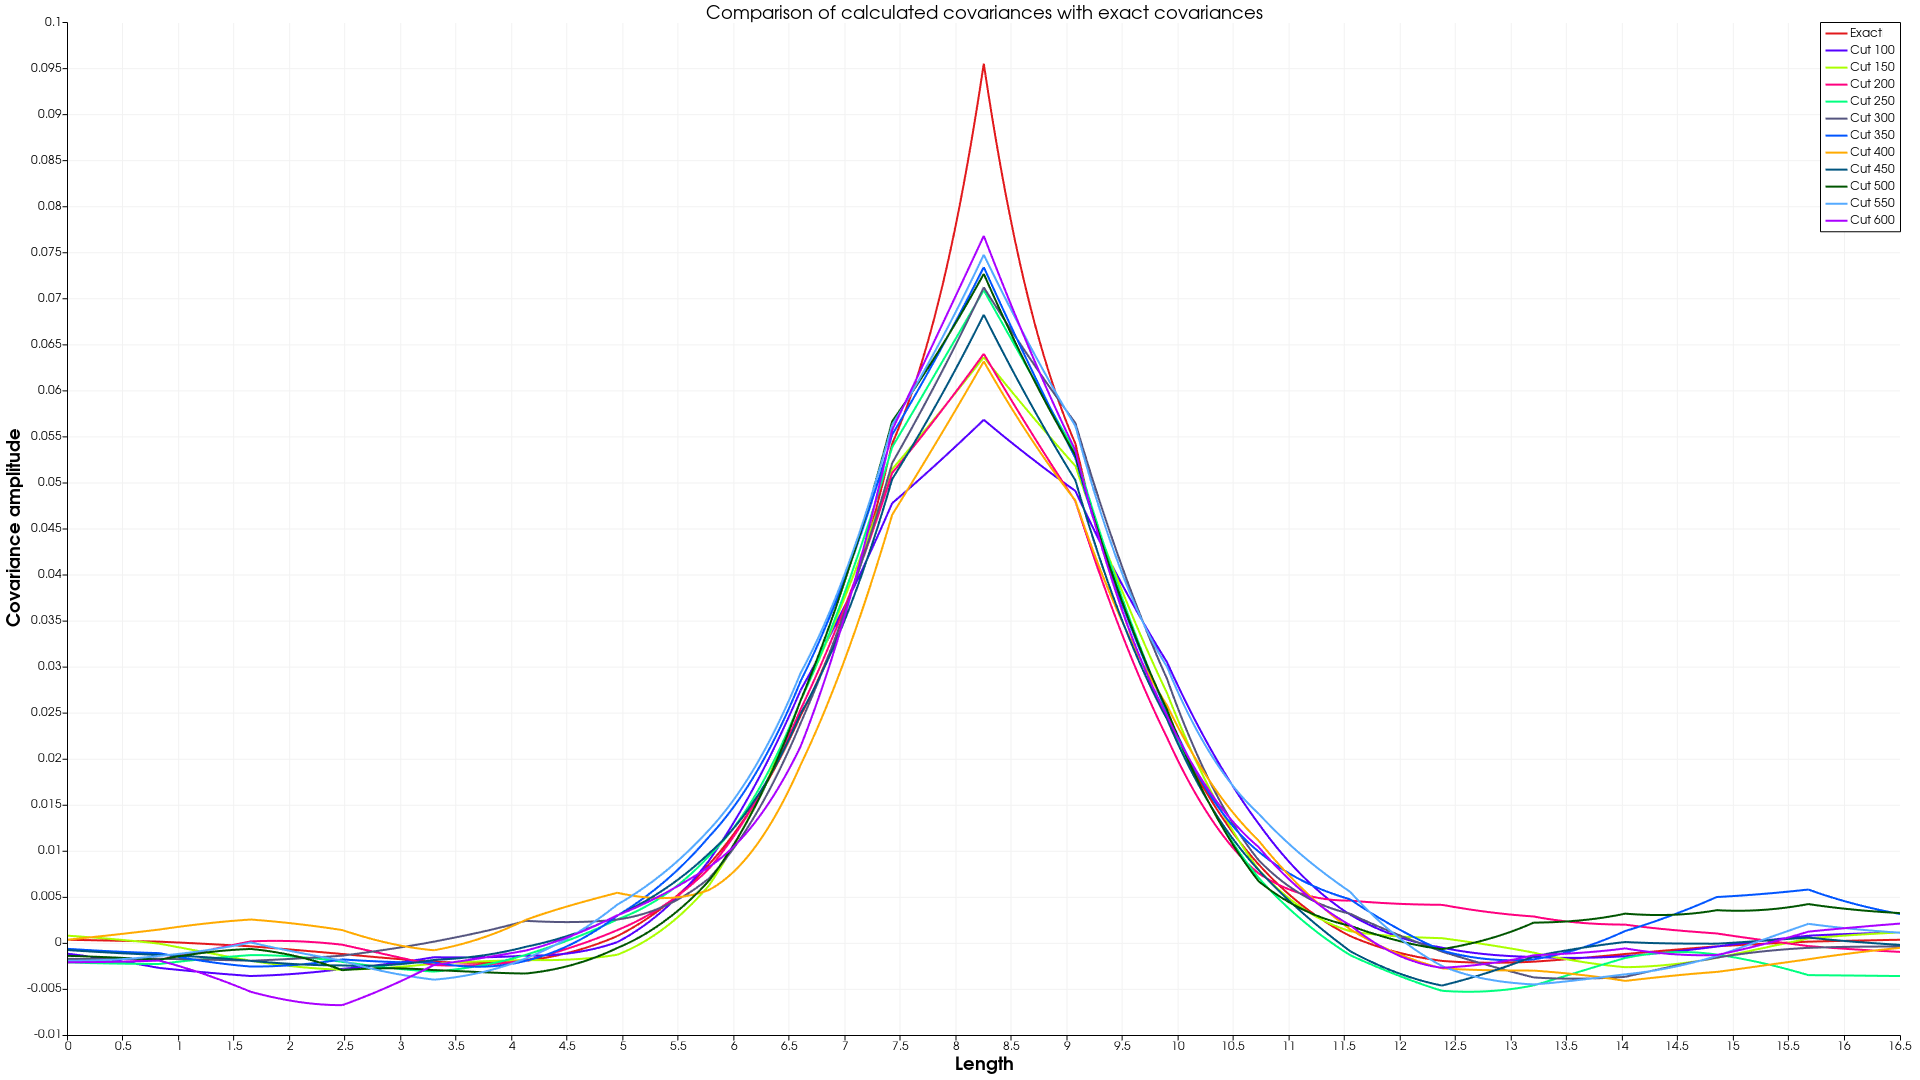
\includegraphics[width=0.4\linewidth]{comparison_covcut0_diag}}%
        \hfill       
        \subcaptionbox{$x$ направление\label{img:comparison_covcut0_x}} 
        {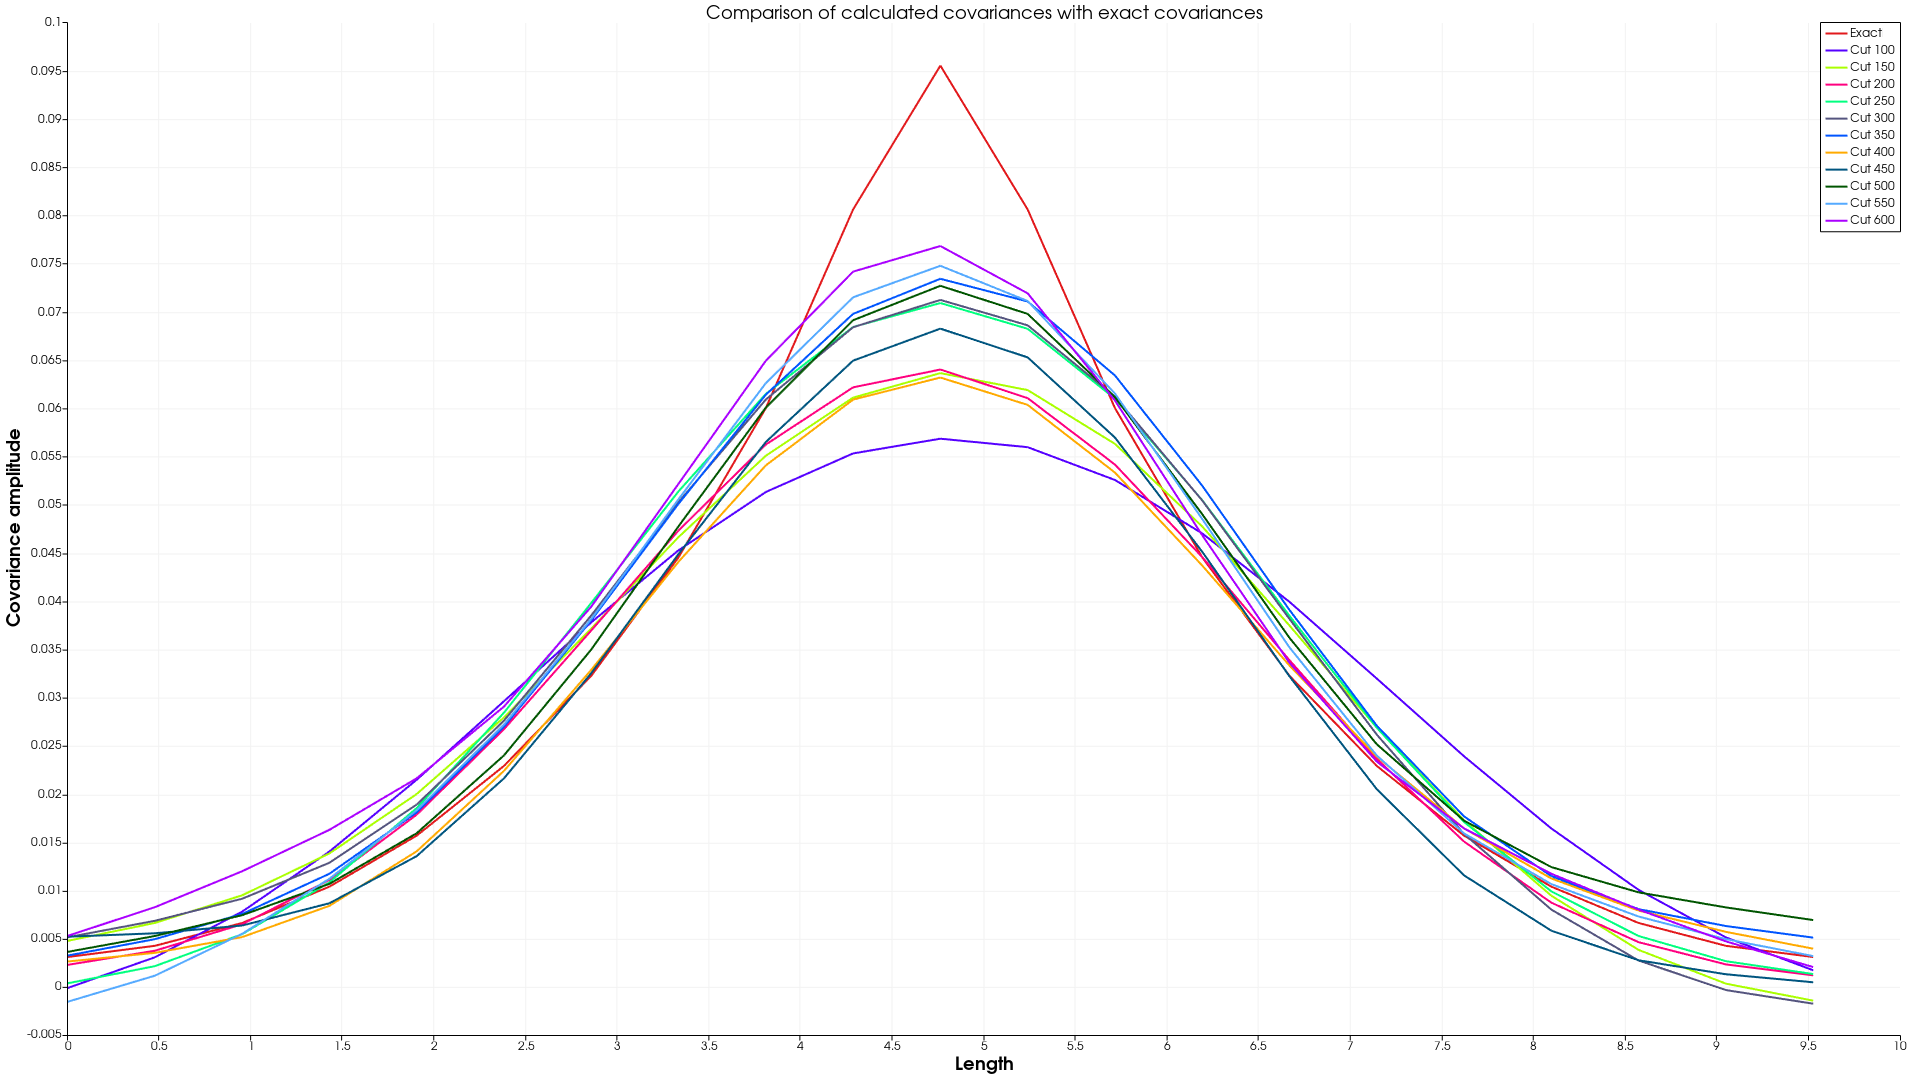
\includegraphics[width=0.4\linewidth]{comparison_covcut0_x}} \\
        \hfill
        \subcaptionbox[List-of-Figures entry]{$y$ направление\label{img:comparison_covcut0_y}} 
        {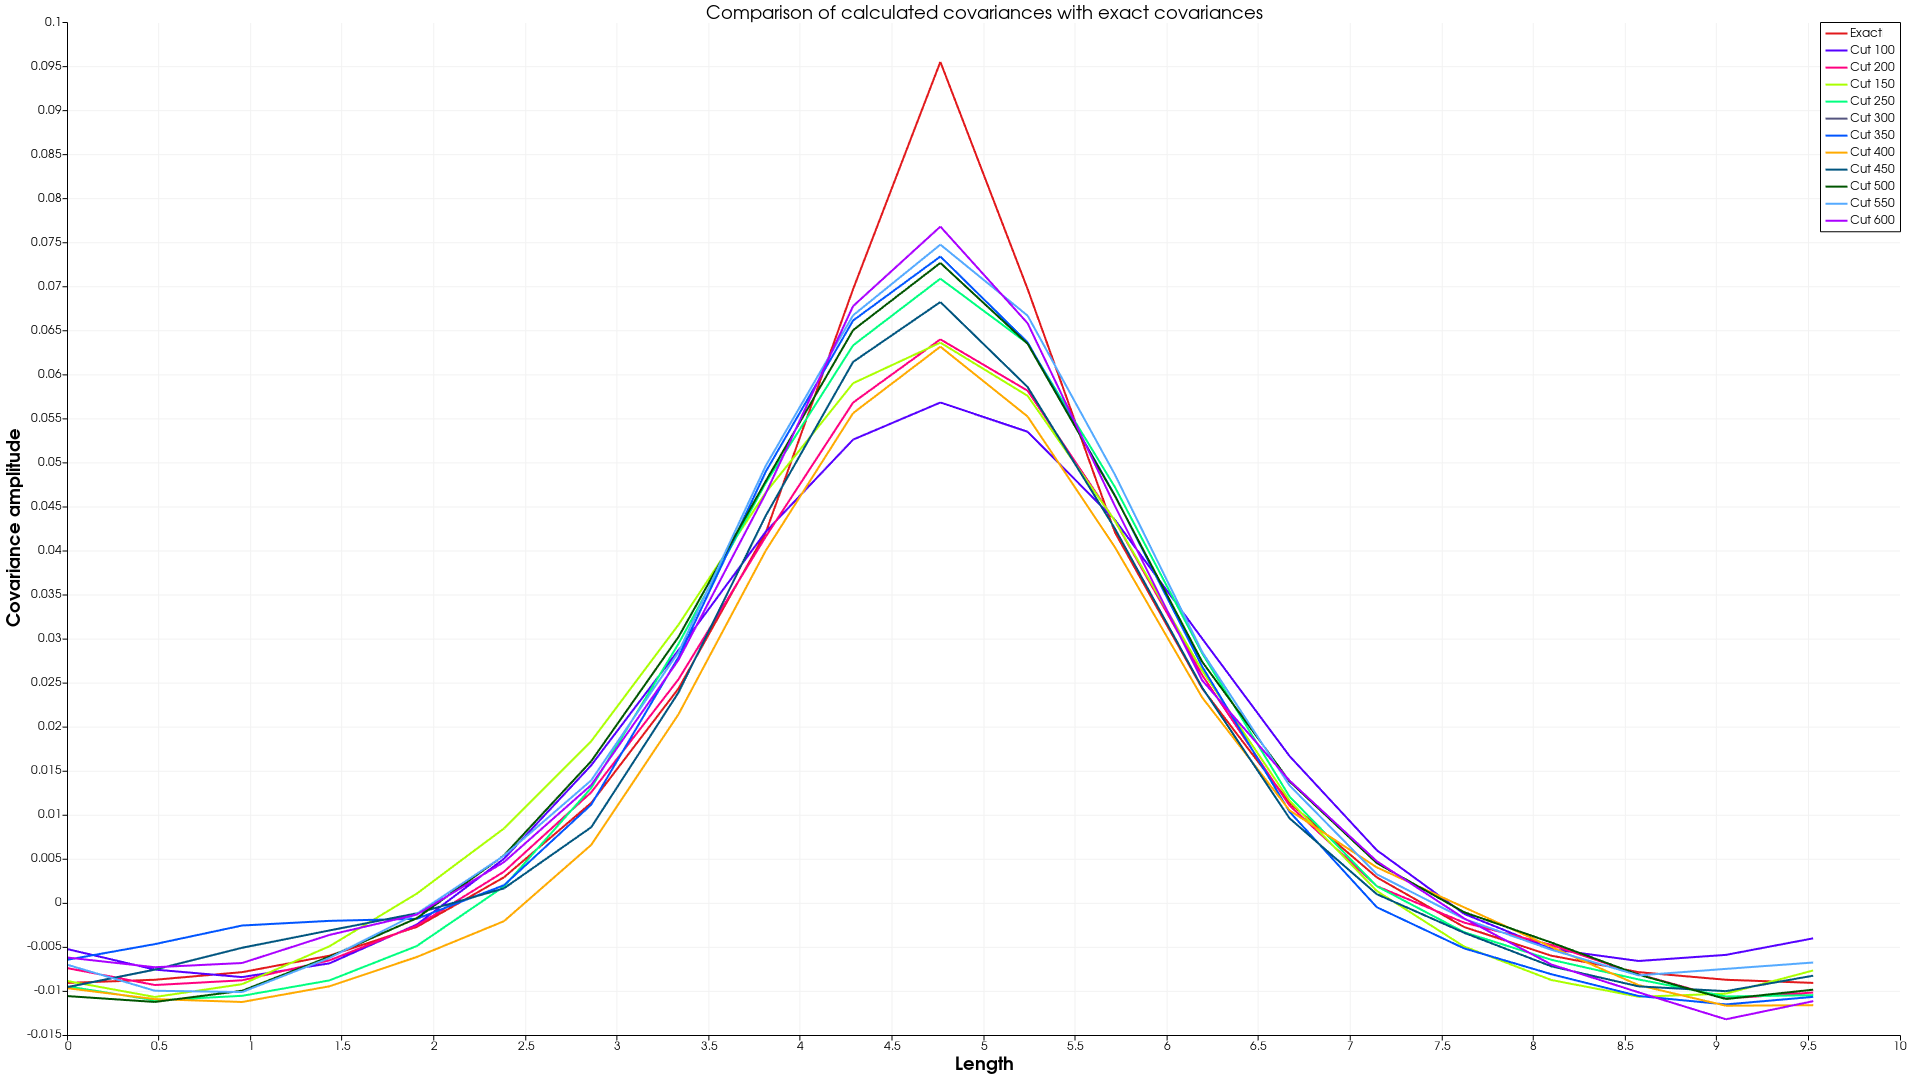
\includegraphics[width=0.4\linewidth]{comparison_covcut0_y}}%
        \hfill       
        \subcaptionbox{$z$ направление\label{img:comparison_covcut0_z}} 
        {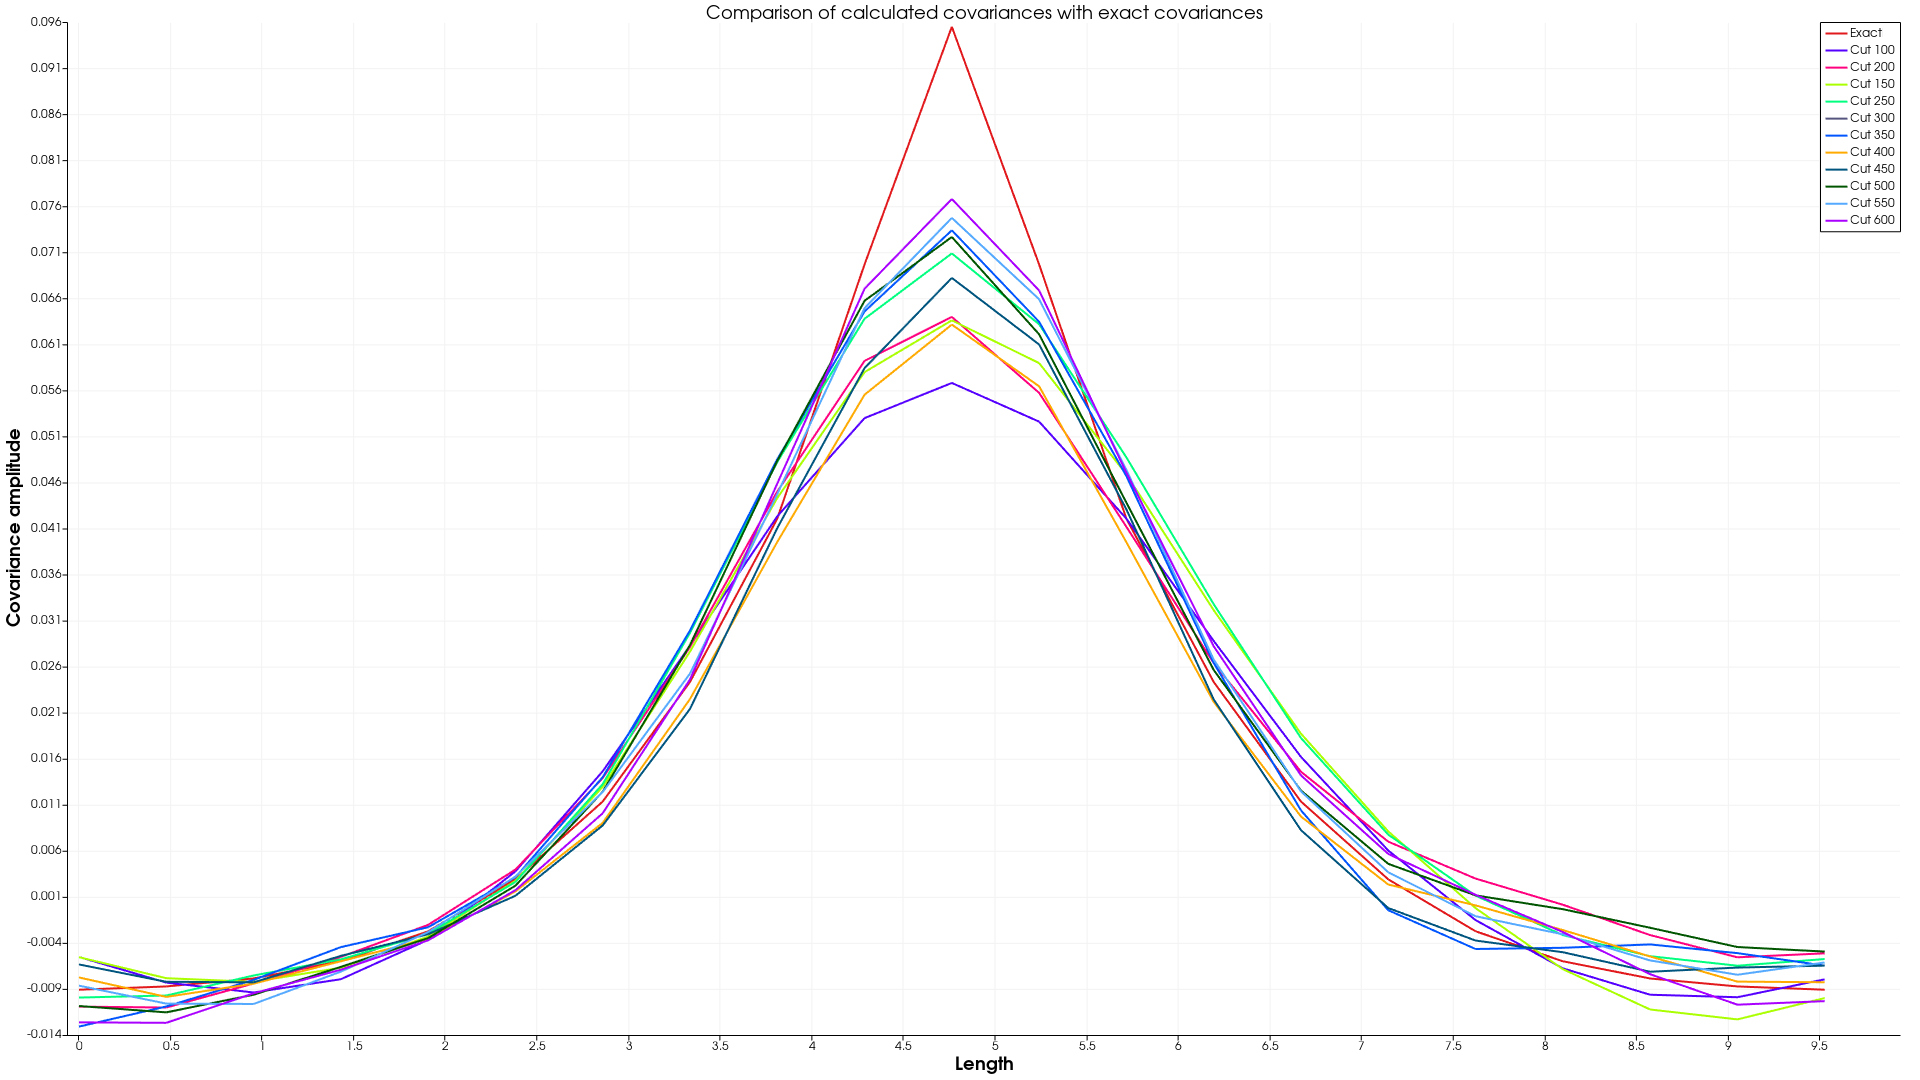
\includegraphics[width=0.4\linewidth]{comparison_covcut0_z}}
        \hfill
    }
    
    \onehalfspacing{Сравнение ковариацинной функции, допуск 0\%, для направлений а) вдоль диагонали, б) вдоль оси $x$, в) вдоль оси $y$, г) вдоль оси $z$}
    \caption{Сравнение ковариационной функции для допуска по амплитуде ковариаций в 0\% для различных направлений в рассматриваемой области}
    \label{img:covcut_0_comparison}  
\end{figure}
%
% Обрезание 1%
%
\begin{figure}[!h]
    \center{
        \hfill
        \subcaptionbox[List-of-Figures entry]{диагональ\label{img:comparison_covcut1_diag}} 
        {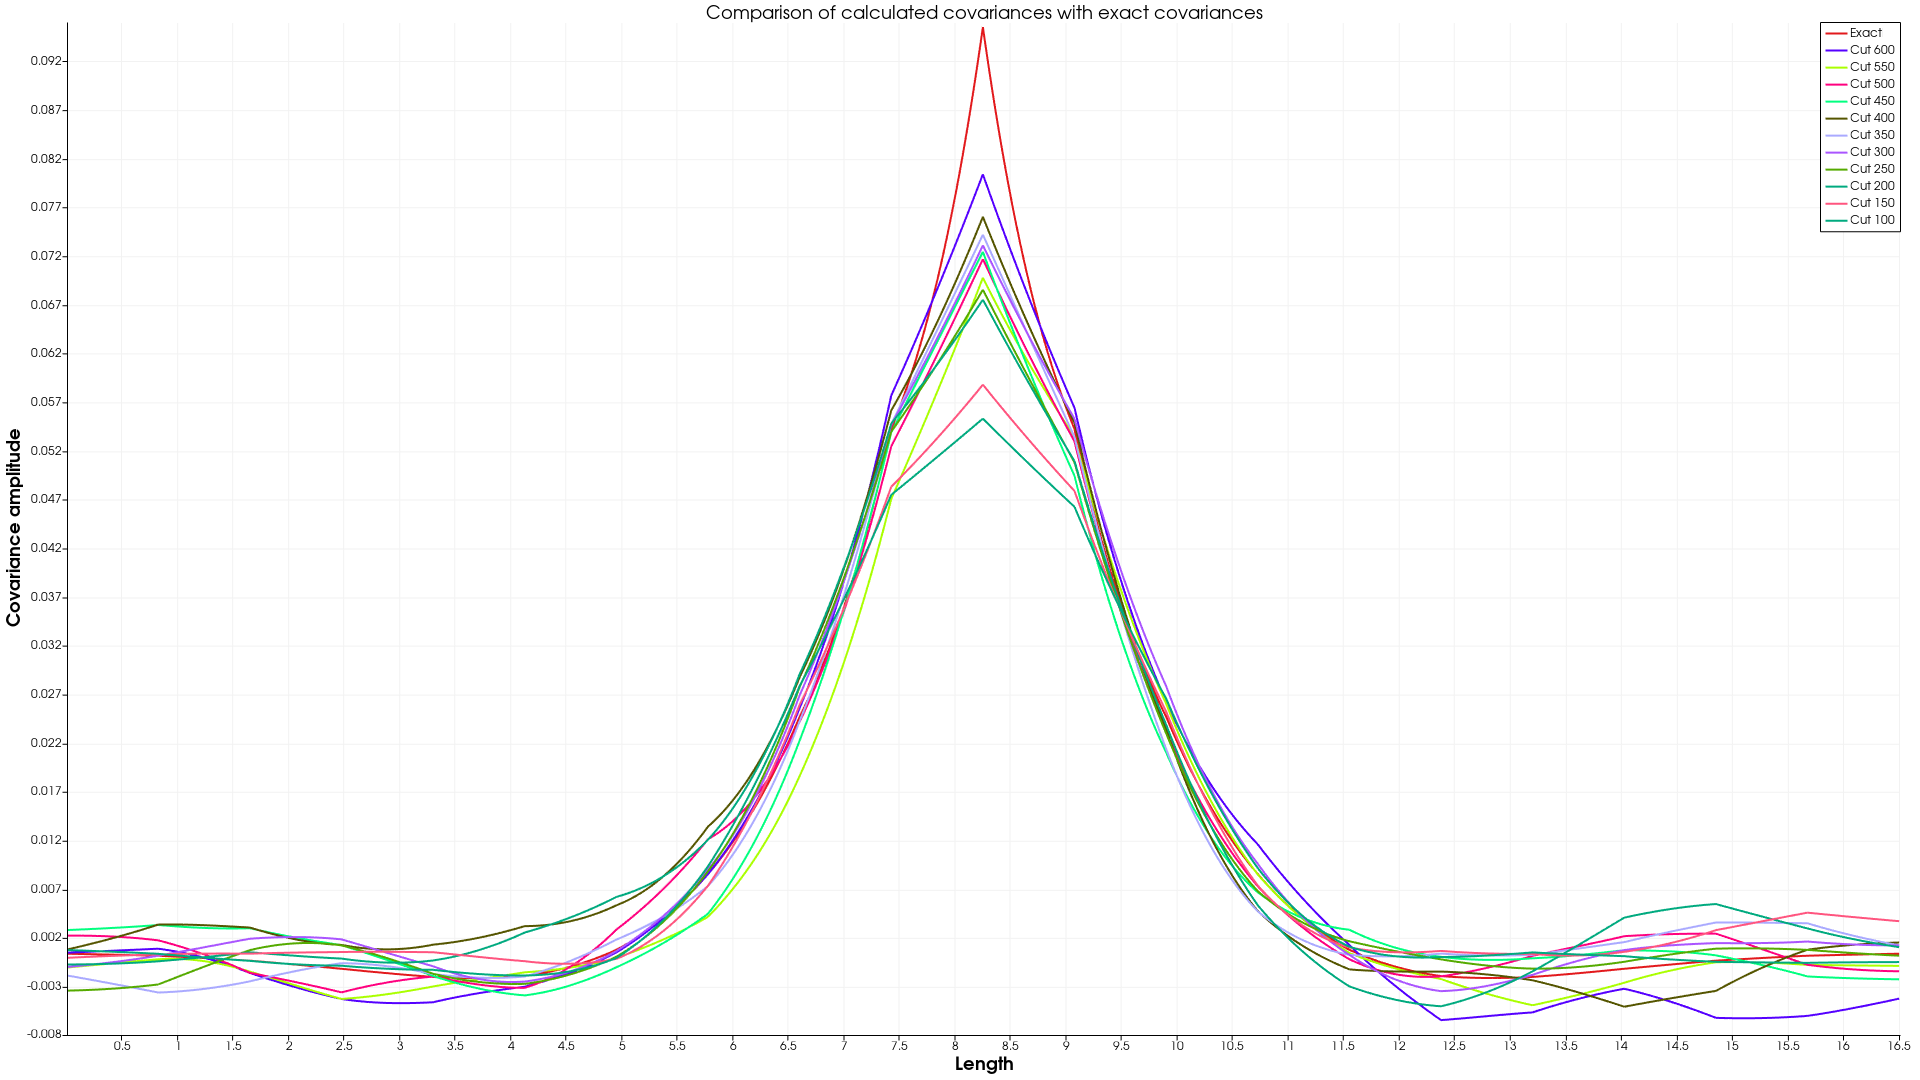
\includegraphics[width=0.4\linewidth]{comparison_covcut1_diag}}%
        \hfill       
        \subcaptionbox{$x$ направление\label{img:comparison_covcut1_x}} 
        {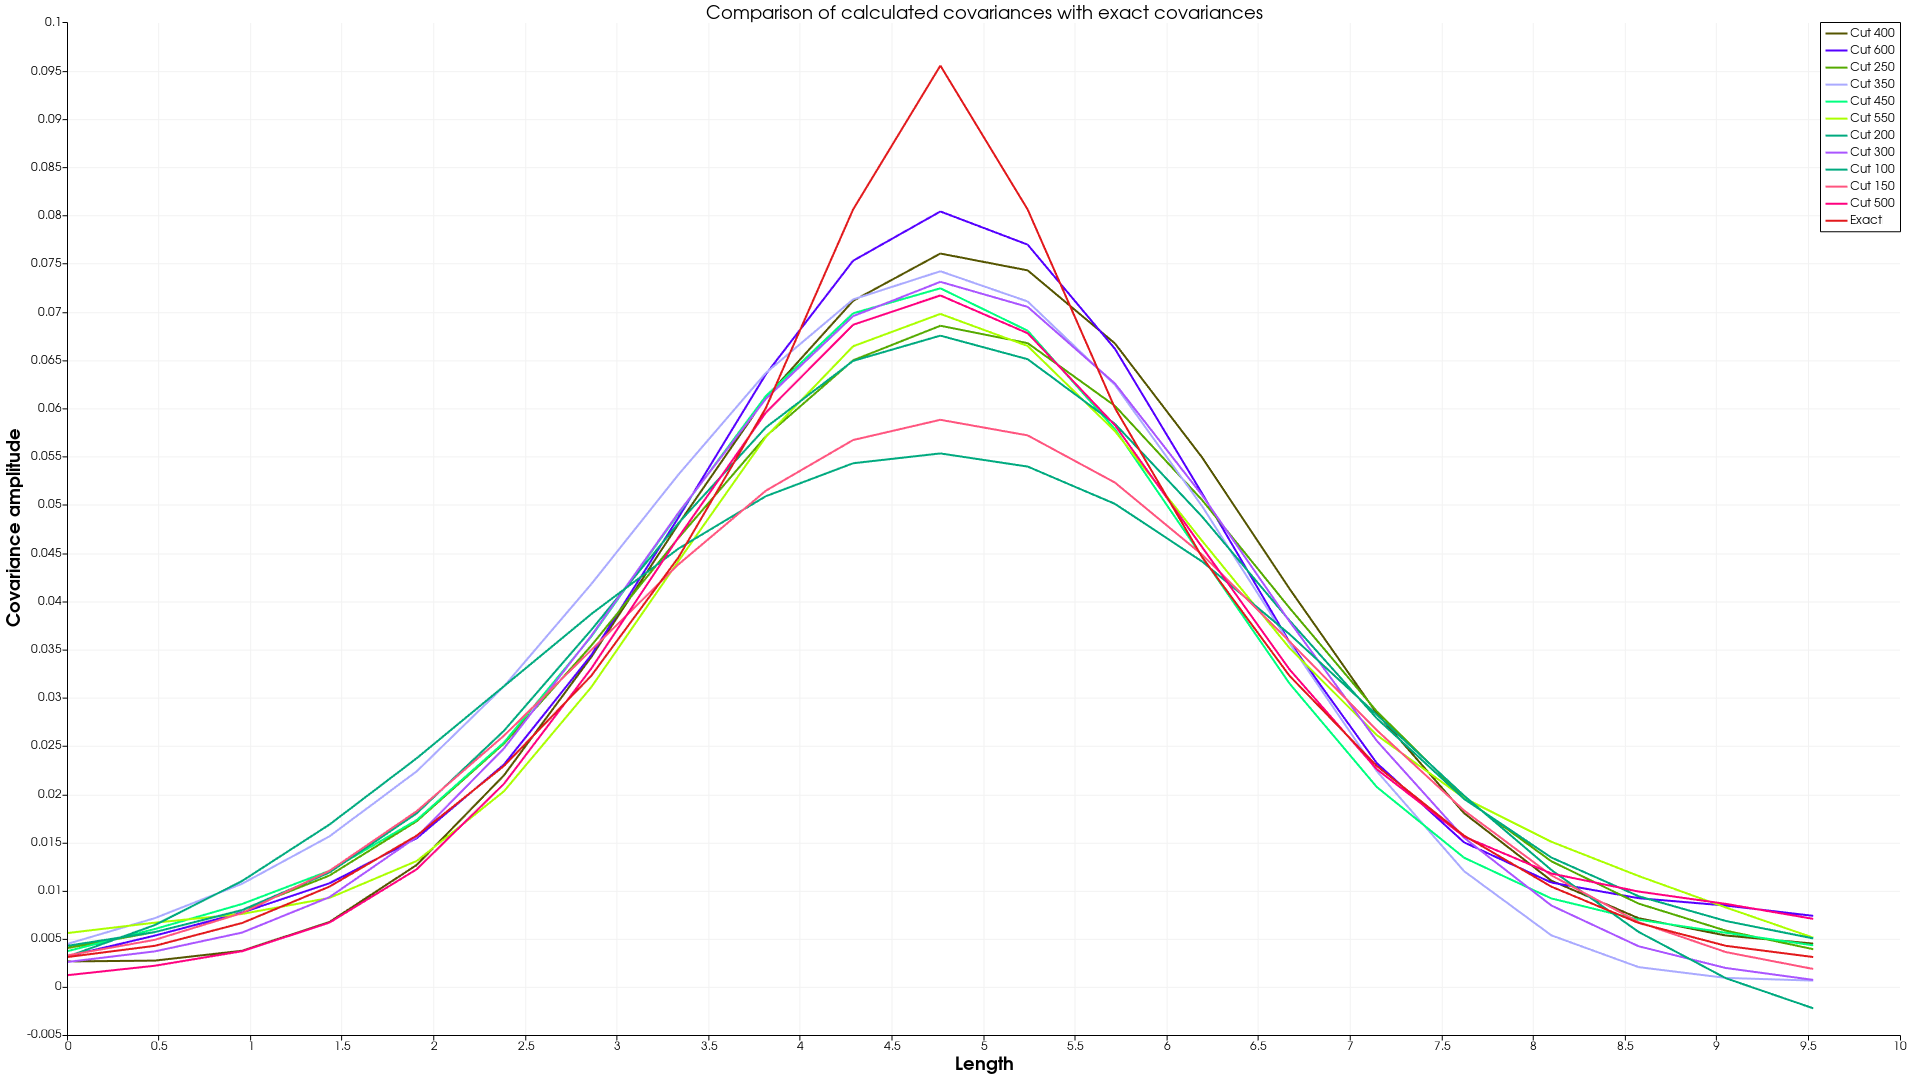
\includegraphics[width=0.4\linewidth]{comparison_covcut1_x}} \\
        \hfill
        \subcaptionbox[List-of-Figures entry]{$y$ направление\label{img:comparison_covcut1_y}} 
        {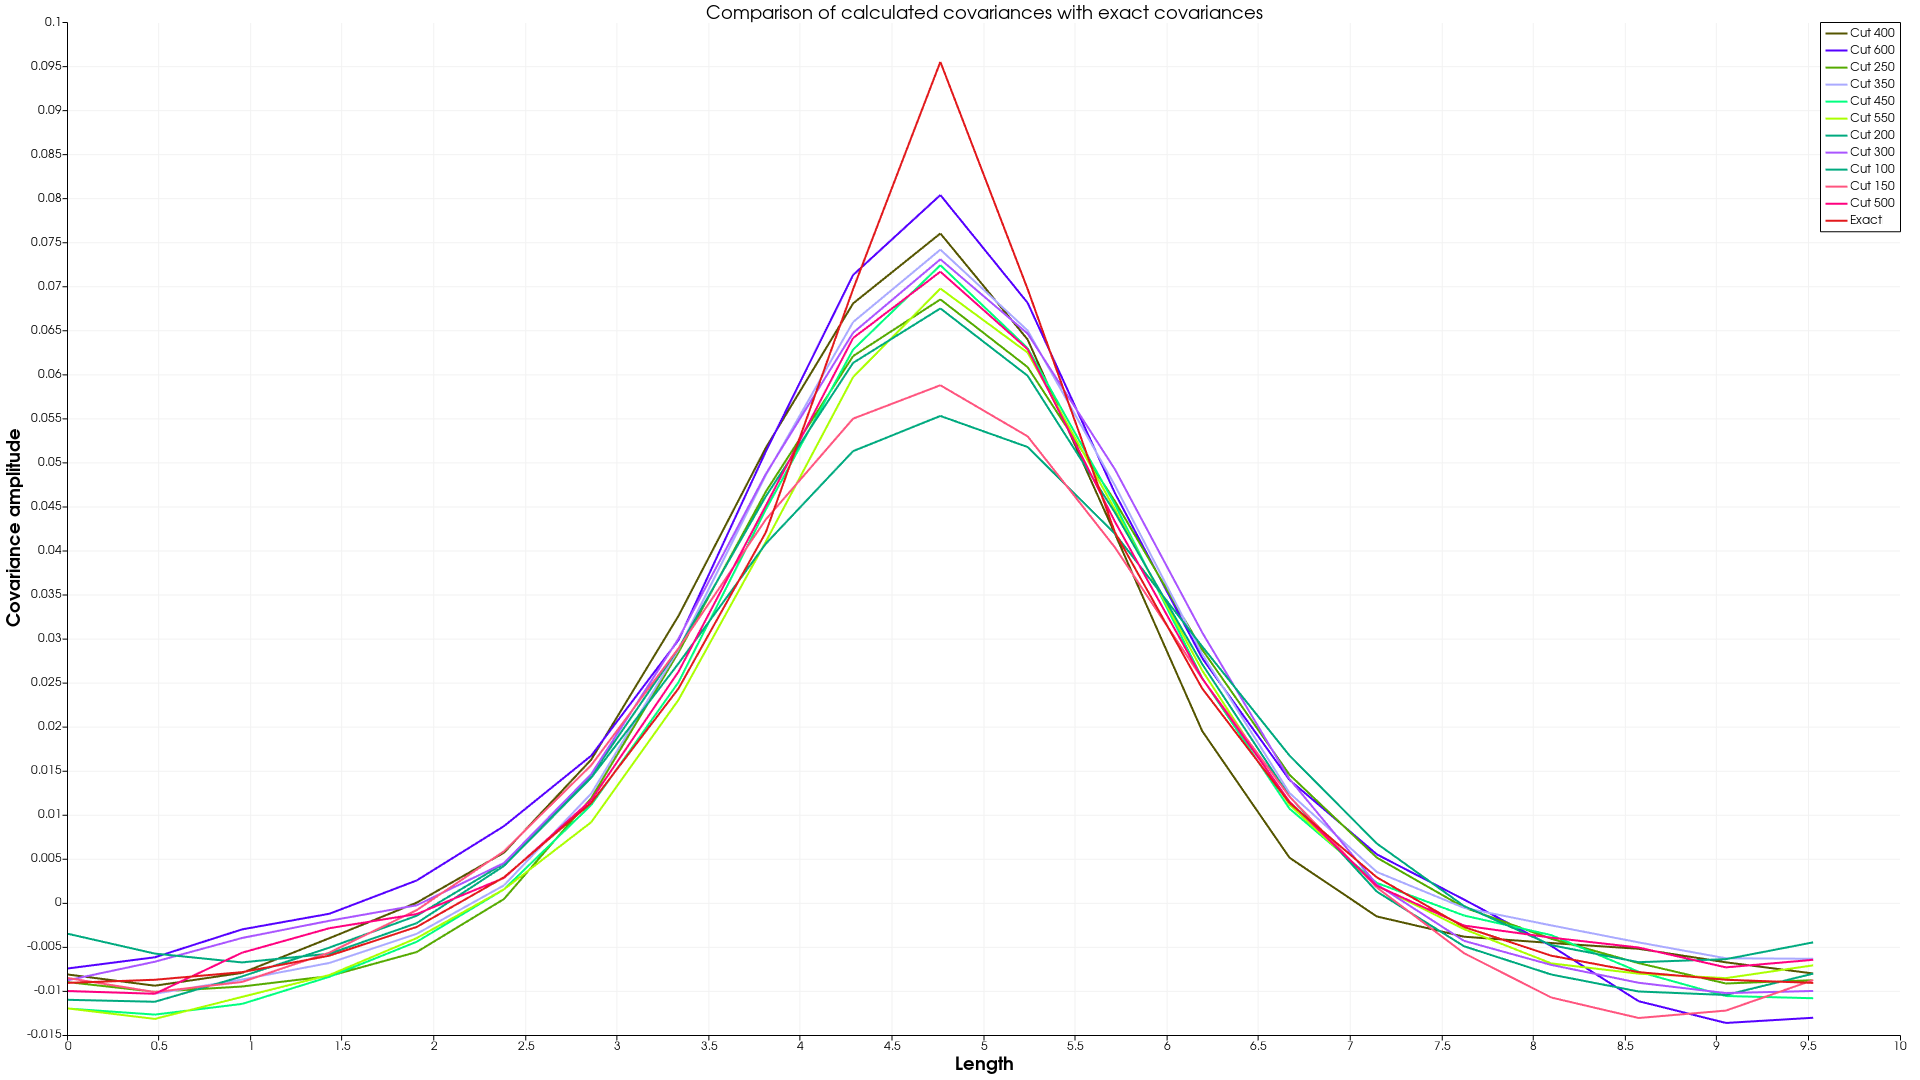
\includegraphics[width=0.4\linewidth]{comparison_covcut1_y}}%
        \hfill       
        \subcaptionbox{$z$ направление\label{img:comparison_covcut1_z}} 
        {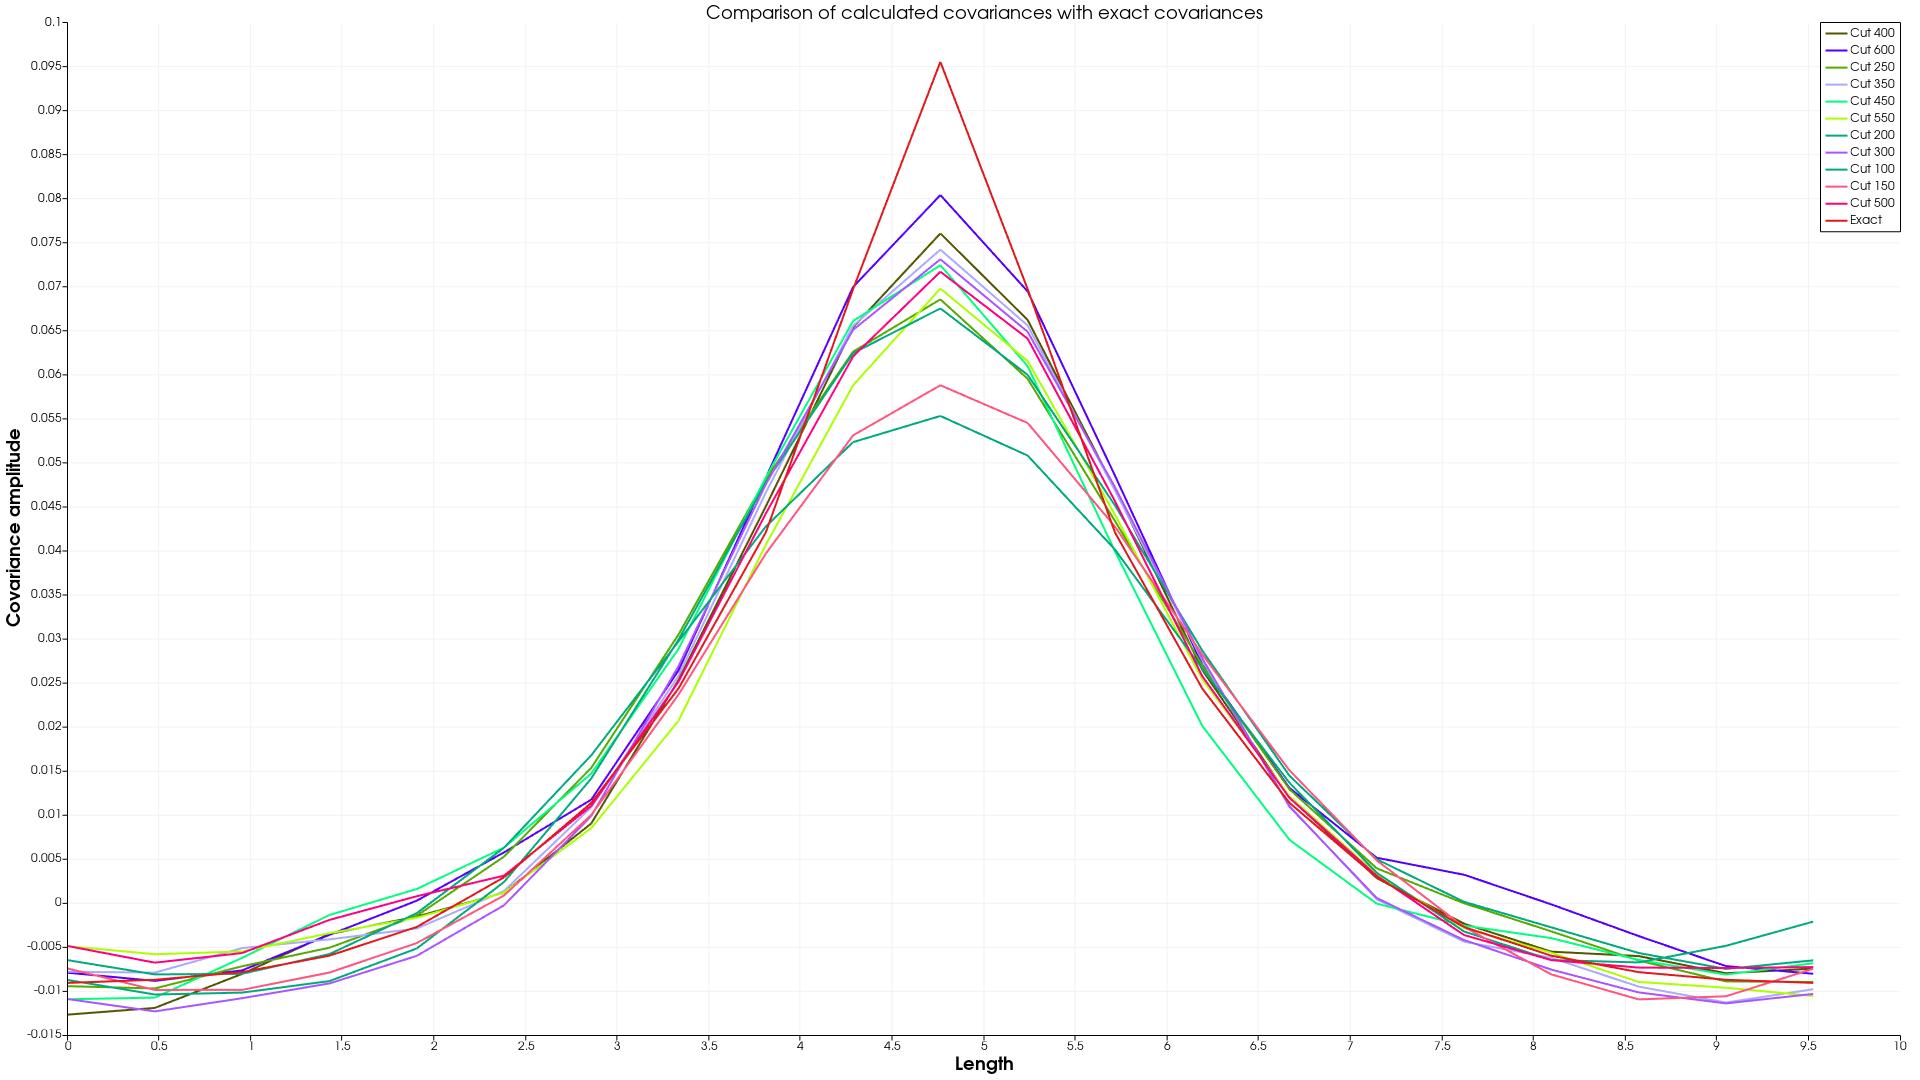
\includegraphics[width=0.4\linewidth]{comparison_covcut1_z}}
        \hfill
    }
    
    \onehalfspacing{Сравнение ковариацинной функции, допуск 1\%, для направлений а) вдоль диагонали, б) вдоль оси $x$, в) вдоль оси $y$, г) вдоль оси $z$}
    \caption{Сравнение ковариационной функции для допуска по амплитуде ковариаций в 1\% для различных направлений в рассматриваемой области}
    \label{img:covcut_1_comparison}  
\end{figure}
%
% Обрезание 2%
%
\begin{figure}[!h]
    \center{
        \hfill
        \subcaptionbox[List-of-Figures entry]{диагональ\label{img:comparison_covcut2_diag}} 
        {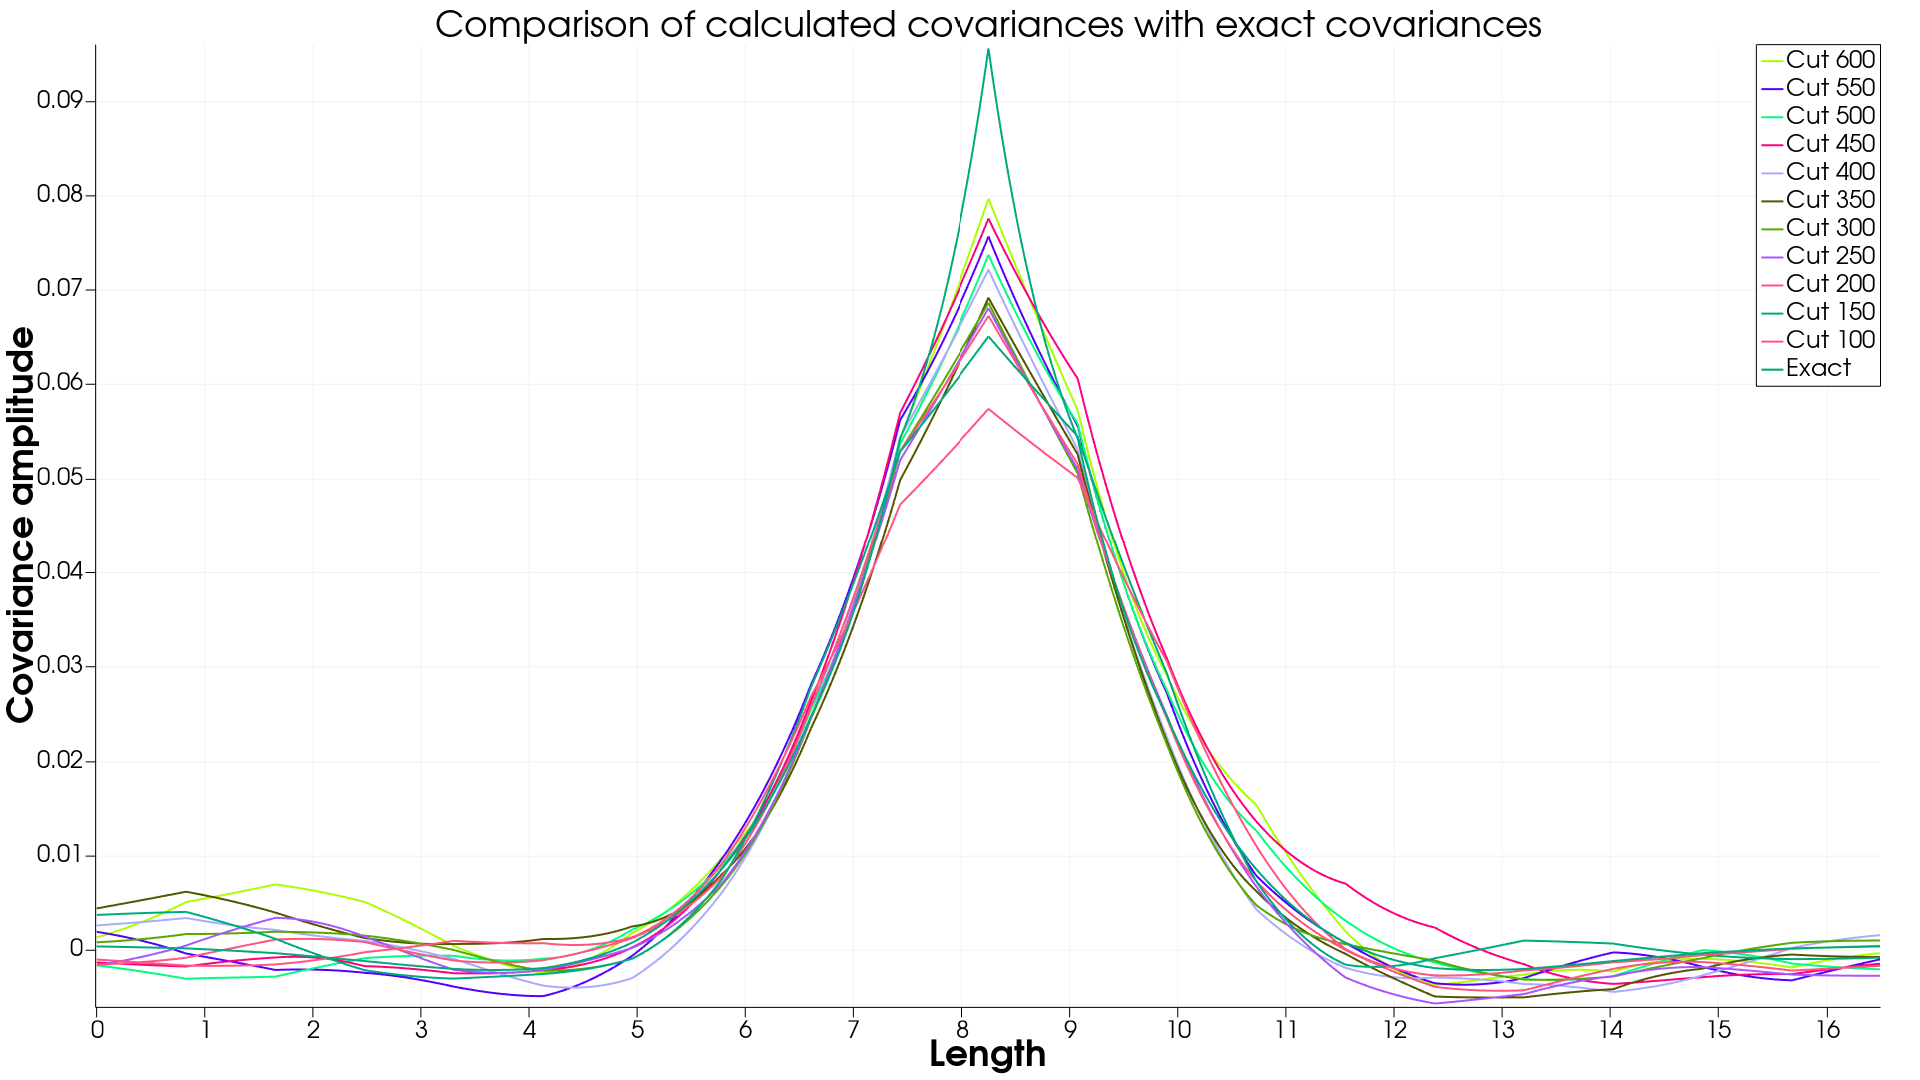
\includegraphics[width=0.4\linewidth]{comparison_covcut2_diag}}%
        \hfill       
        \subcaptionbox{$x$ направление\label{img:comparison_covcut1_x}} 
        {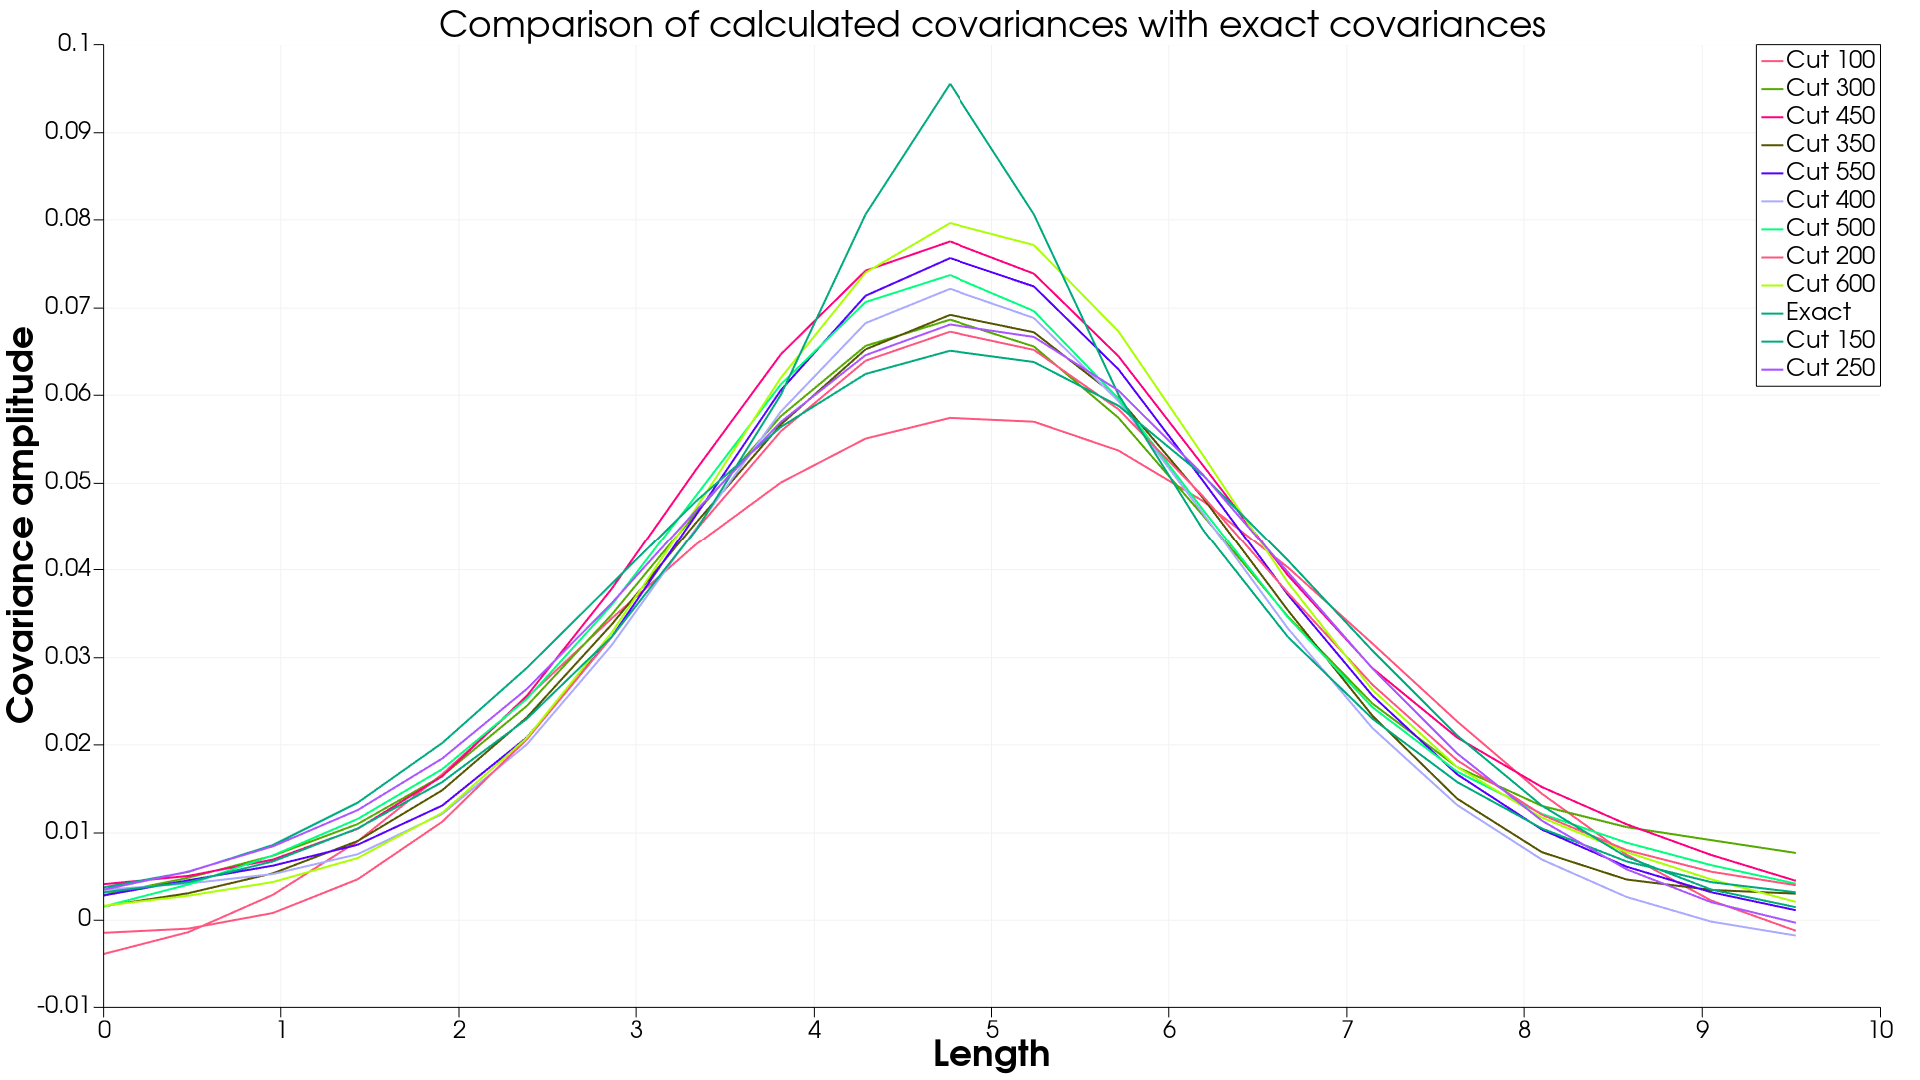
\includegraphics[width=0.4\linewidth]{comparison_covcut2_x}} \\
        \hfill
        \subcaptionbox[List-of-Figures entry]{$y$ направление\label{img:comparison_covcut2_y}} 
        {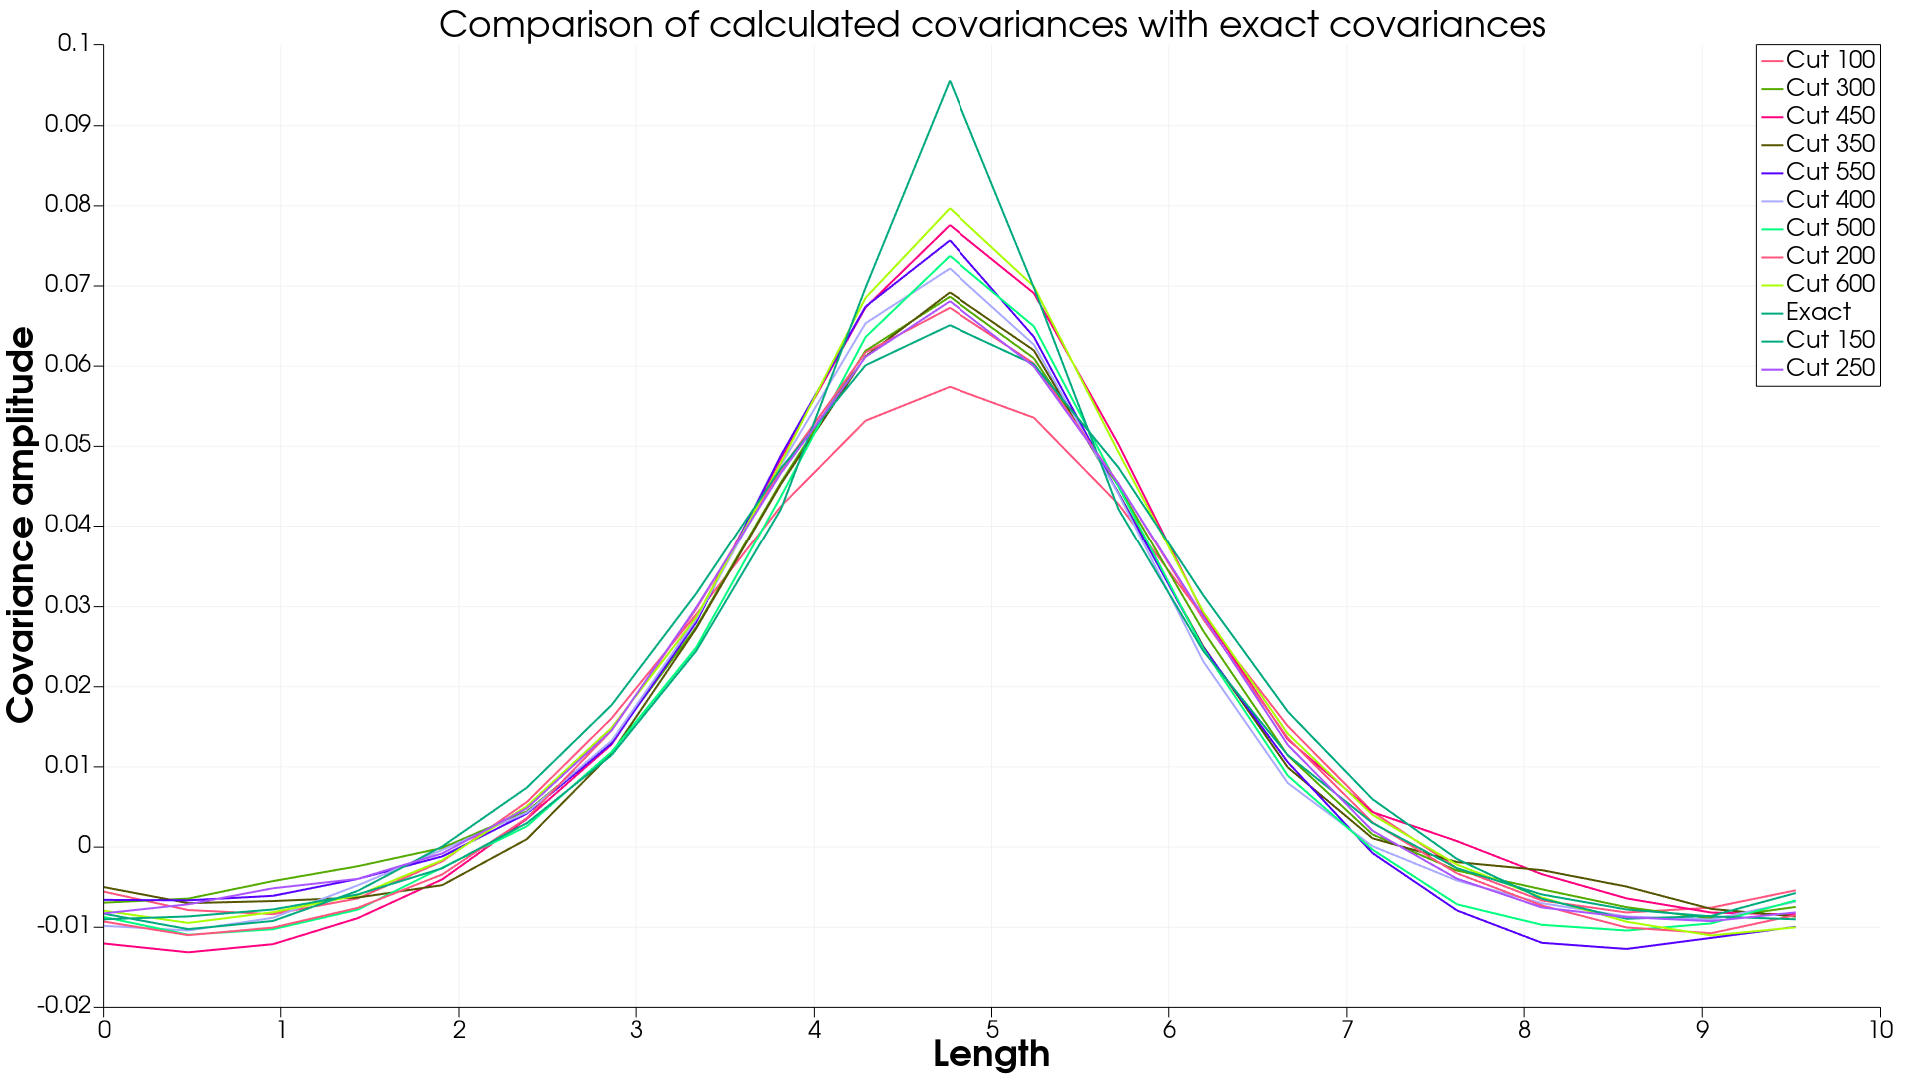
\includegraphics[width=0.4\linewidth]{comparison_covcut2_y}}%
        \hfill       
        \subcaptionbox{$z$ направление\label{img:comparison_covcut2_z}} 
        {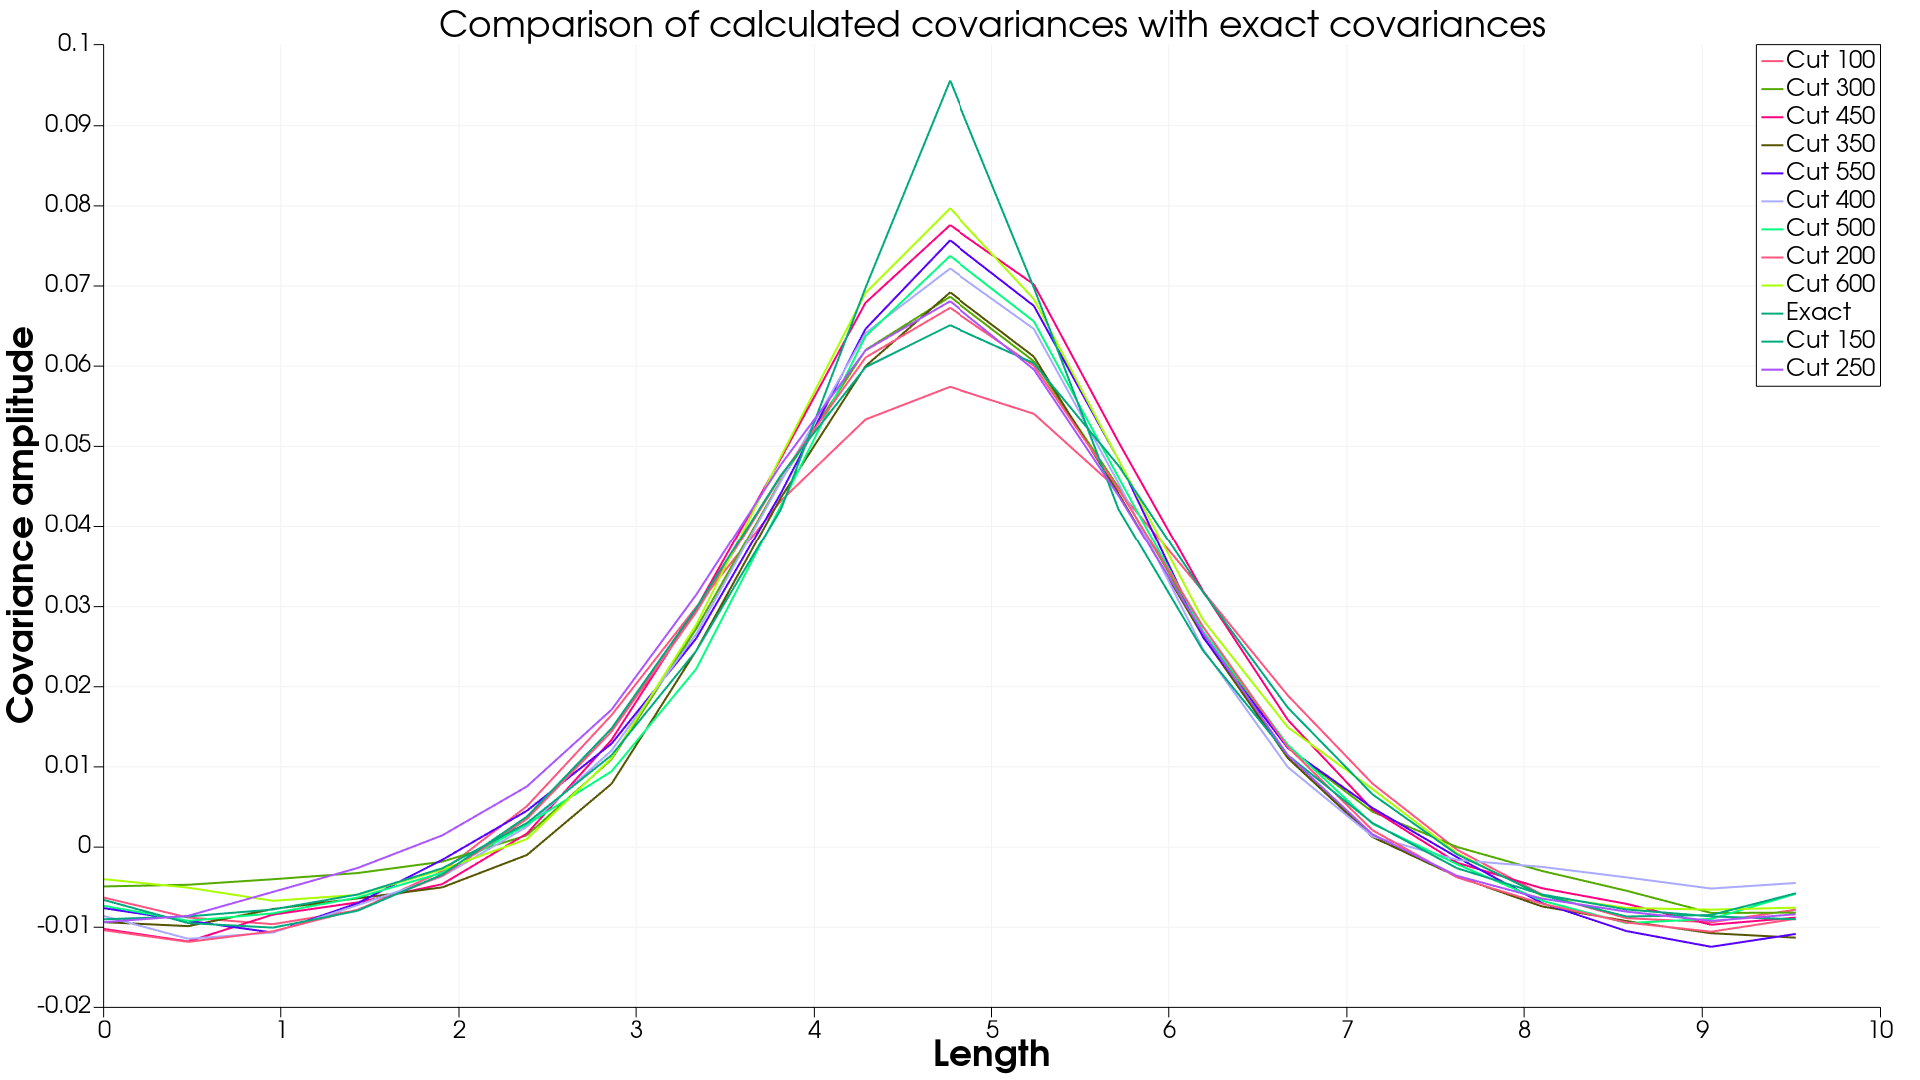
\includegraphics[width=0.4\linewidth]{comparison_covcut2_z}}
        \hfill
    }
    
    \onehalfspacing{Сравнение ковариацинной функции, допуск 2\%, для направлений а) вдоль диагонали, б) вдоль оси $x$, в) вдоль оси $y$, г) вдоль оси $z$}
    \caption{Сравнение ковариационной функции для допуска по амплитуде ковариаций в 2\% для различных направлений в рассматриваемой области}
    \label{img:covcut_2_comparison}  
\end{figure}
%
% Обрезание 3%
%
\begin{figure}[!h]
    \center{
        \hfill
        \subcaptionbox[List-of-Figures entry]{диагональ\label{img:comparison_covcut3_diag}} 
        {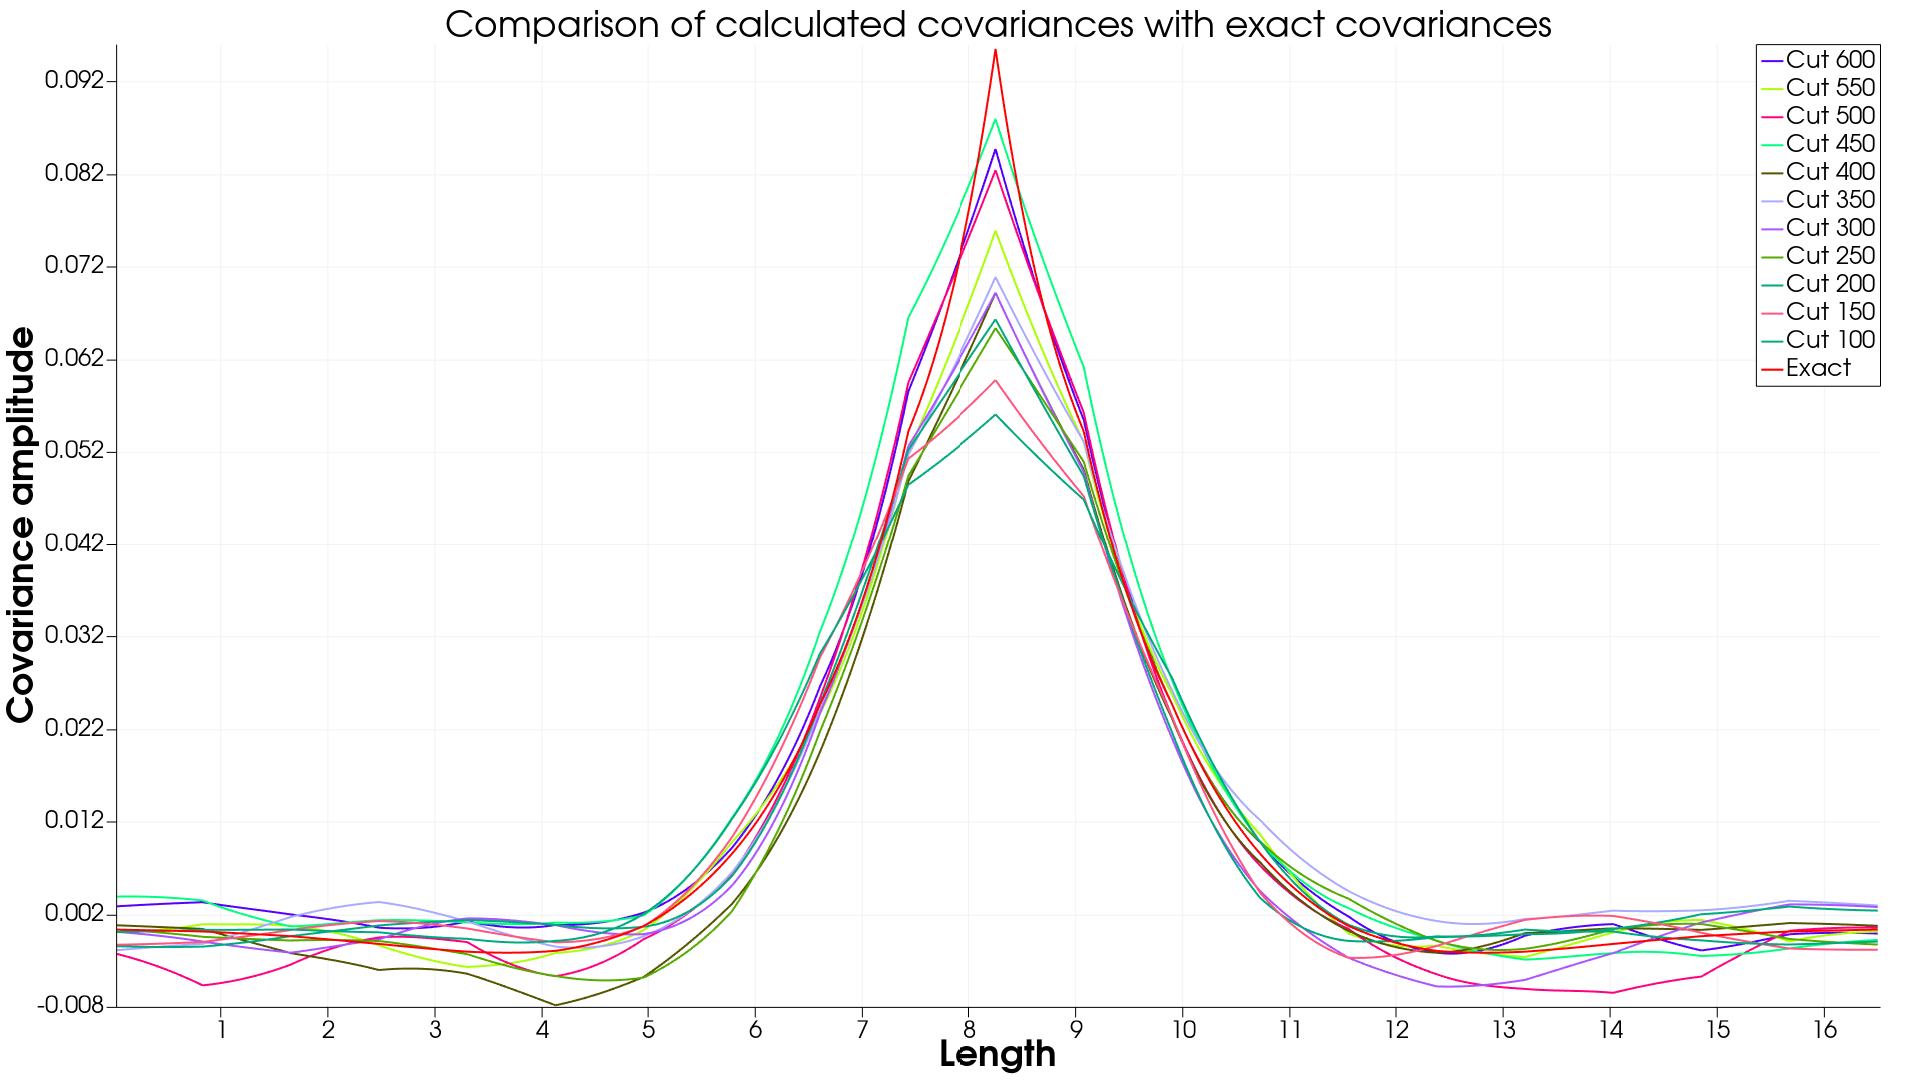
\includegraphics[width=0.4\linewidth]{comparison_covcut3_diag}}%
        \hfill       
        \subcaptionbox{$x$ направление\label{img:comparison_covcut3_x}} 
        {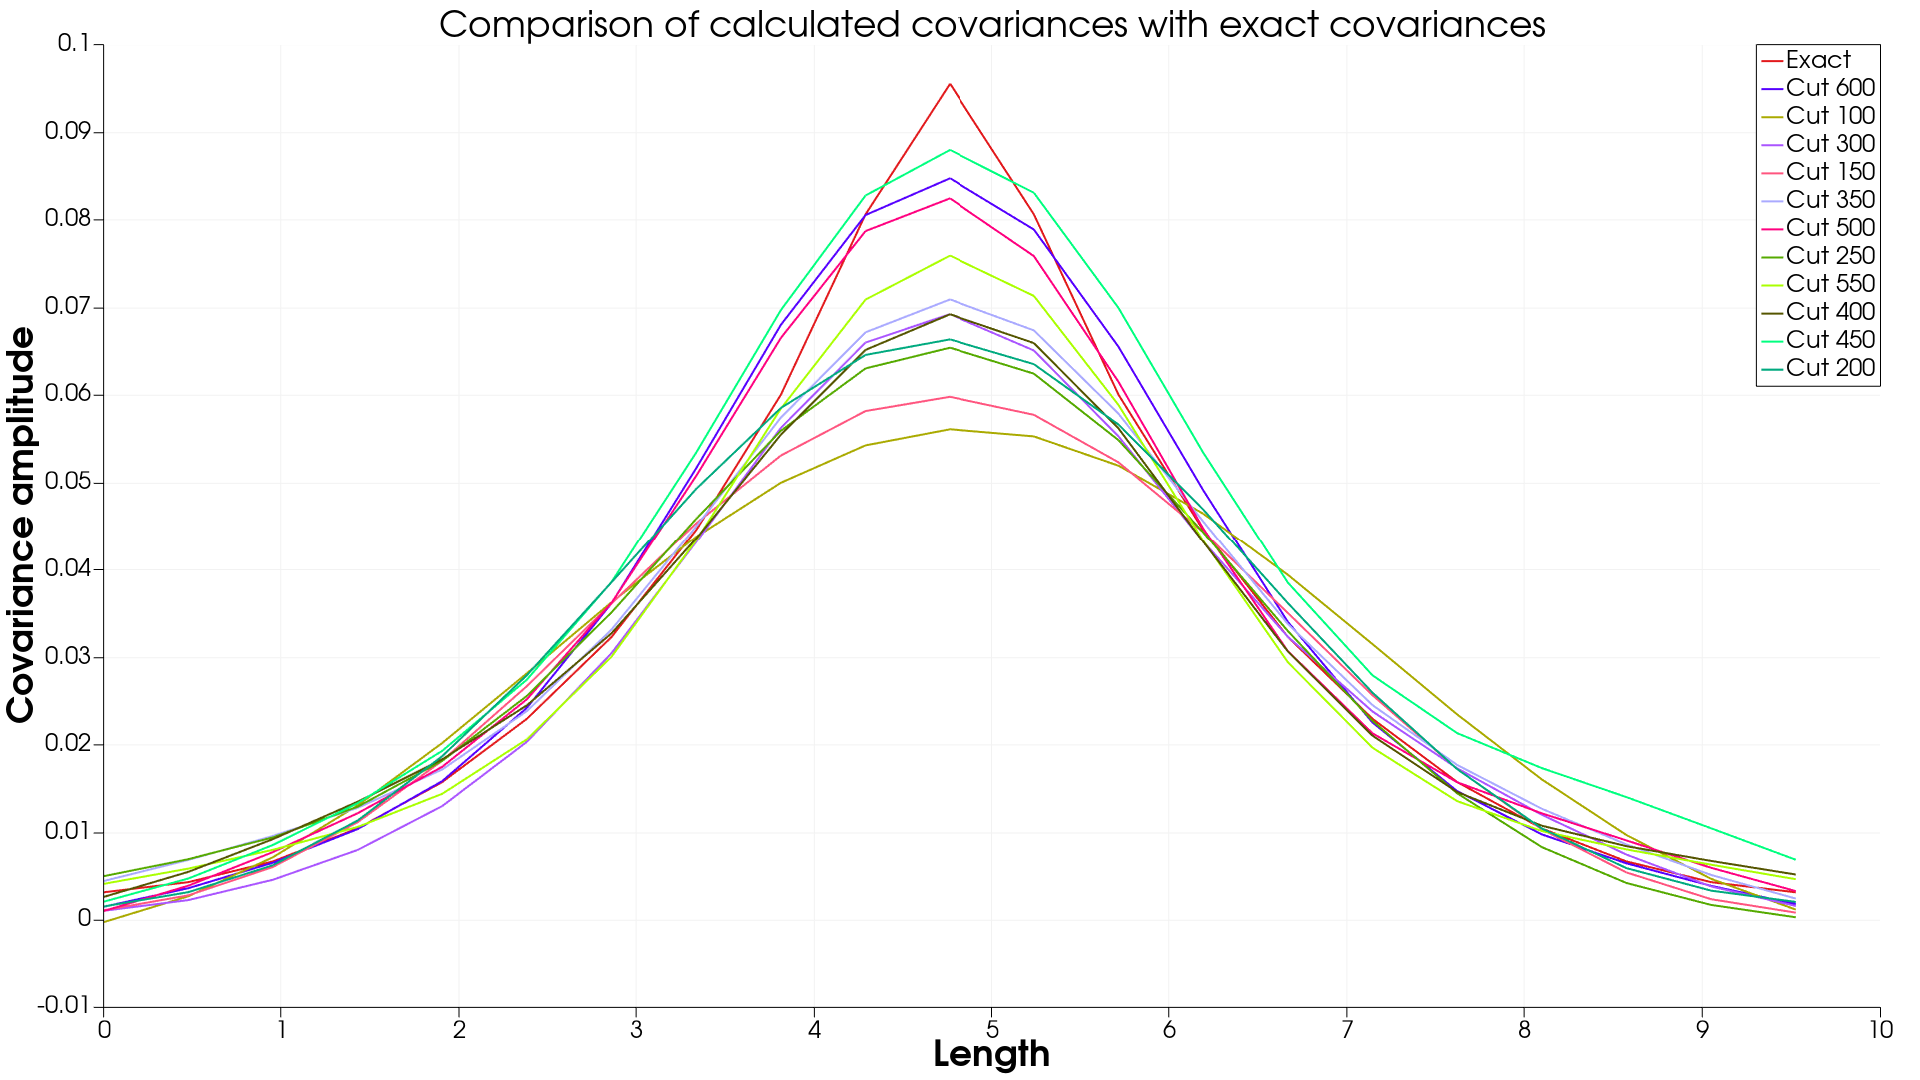
\includegraphics[width=0.4\linewidth]{comparison_covcut3_x}} \\
        \hfill
        \subcaptionbox[List-of-Figures entry]{$y$ направление\label{img:comparison_covcut3_y}} 
        {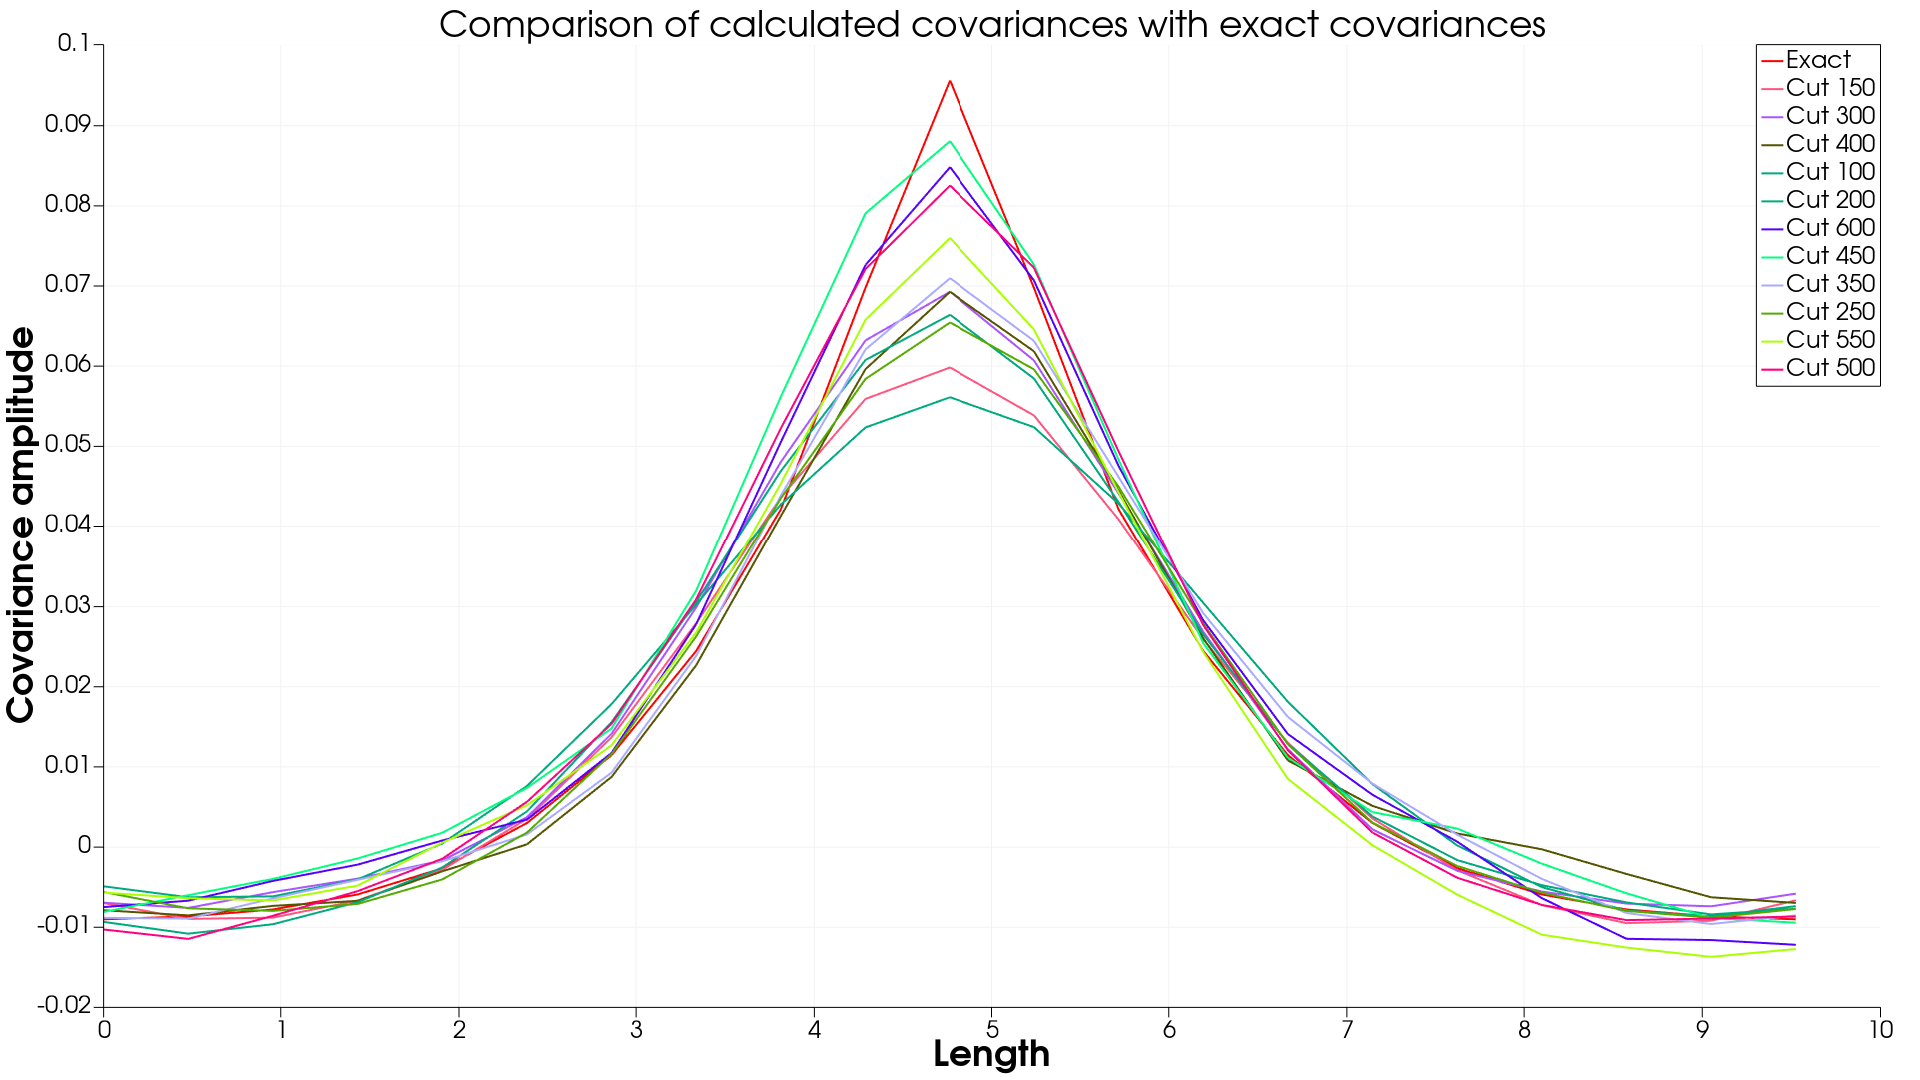
\includegraphics[width=0.4\linewidth]{comparison_covcut3_y}}%
        \hfill       
        \subcaptionbox{$z$ направление\label{img:comparison_covcut3_z}} 
        {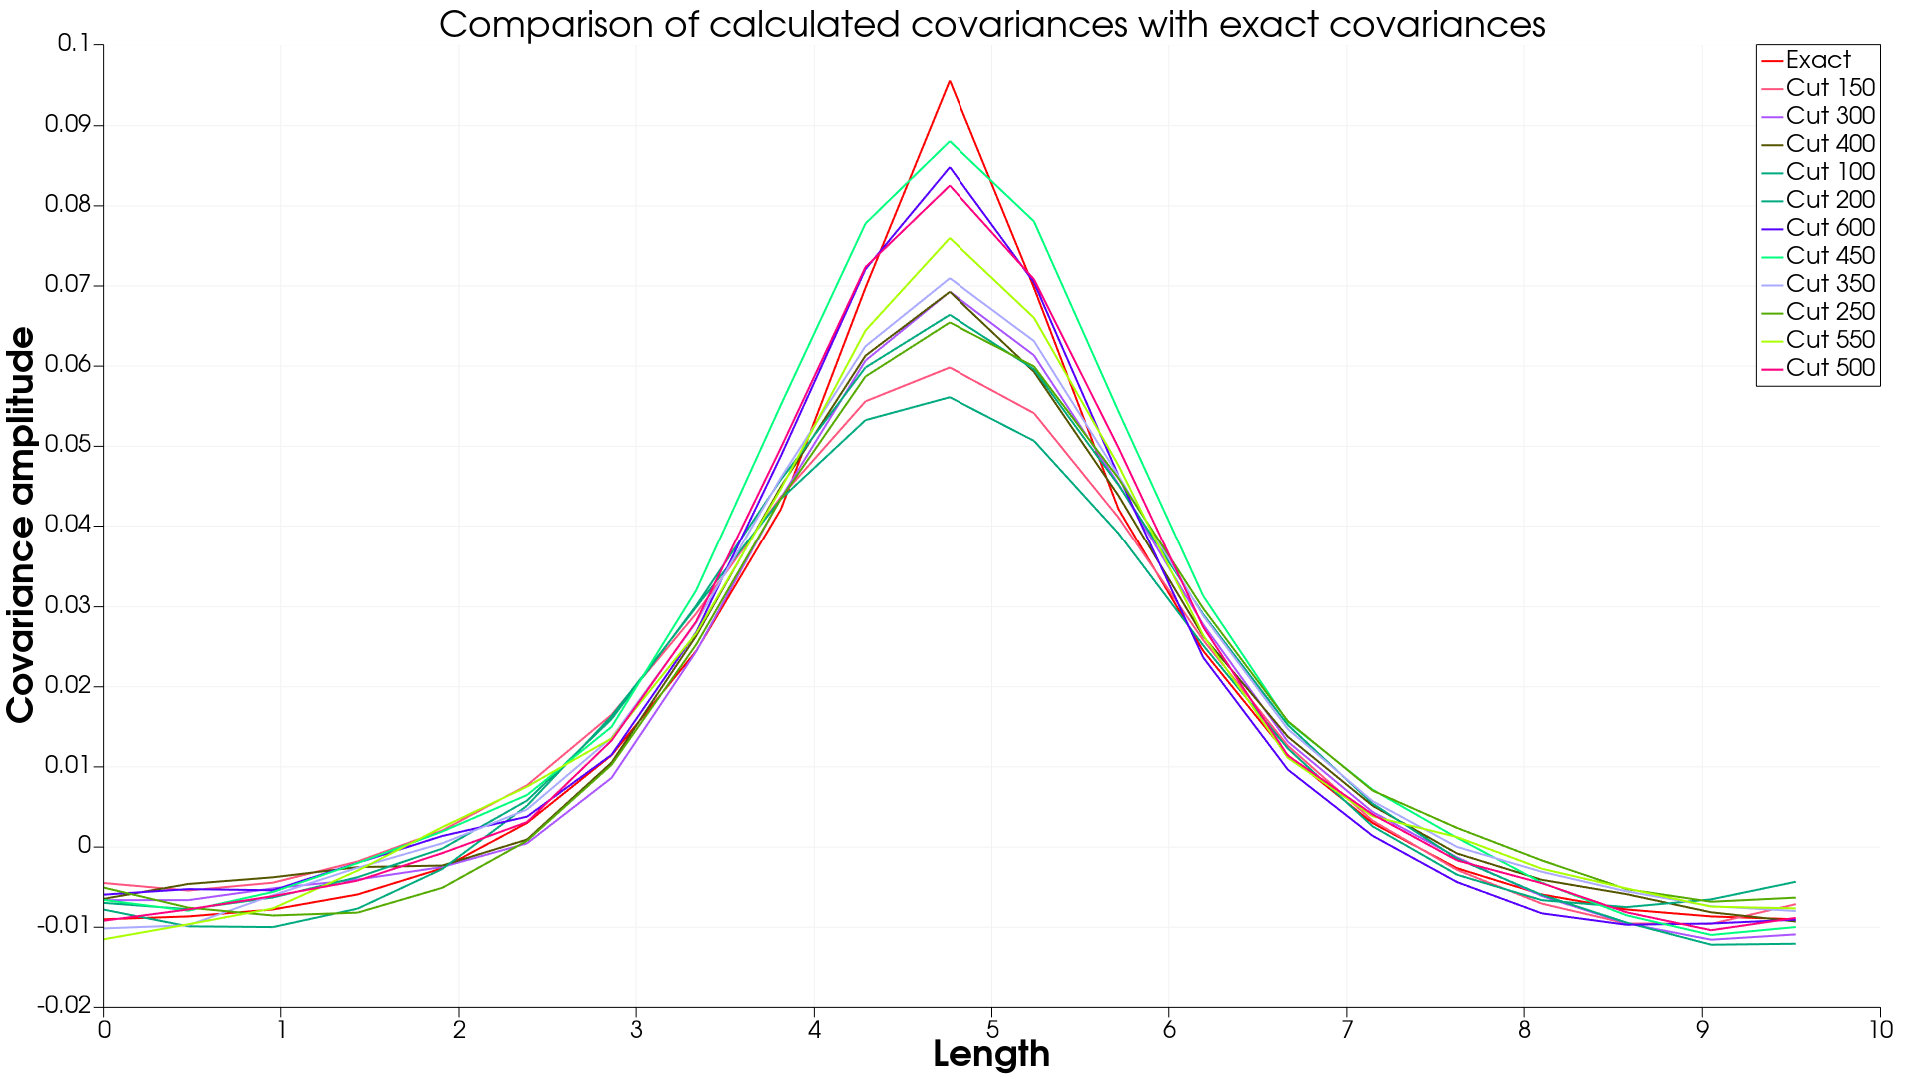
\includegraphics[width=0.4\linewidth]{comparison_covcut3_z}}
        \hfill
    }
    
    \onehalfspacing{Сравнение ковариацинной функции, допуск 3\%, для направлений а) вдоль диагонали, б) вдоль оси $x$, в) вдоль оси $y$, г) вдоль оси $z$}
    \caption{Сравнение ковариационной функции для допуска по амплитуде ковариаций в 3\% для различных направлений в рассматриваемой области}
    \label{img:covcut_3_comparison}  
\end{figure}
%
% Обрезание 4%
%
\begin{figure}[!h]
    \center{
        \hfill
        \subcaptionbox[List-of-Figures entry]{диагональ\label{img:comparison_covcut4_diag}} 
        {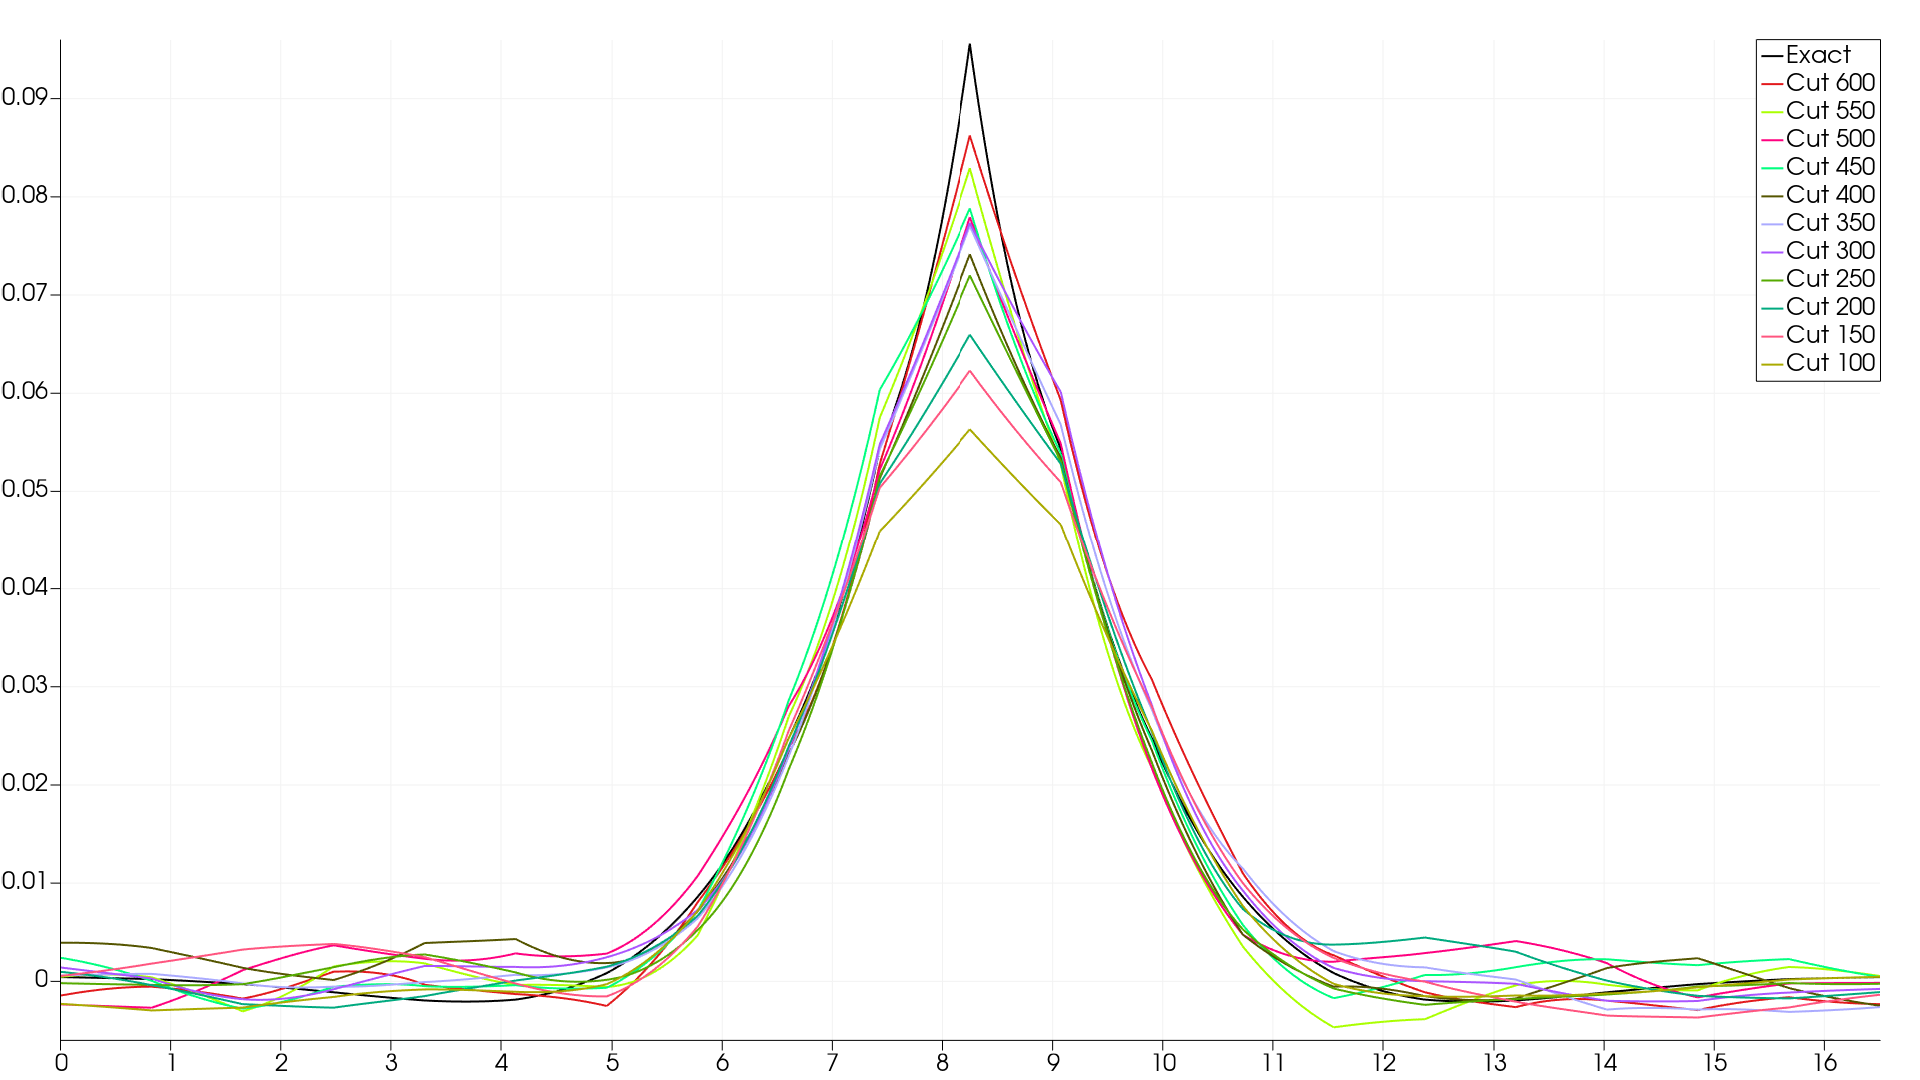
\includegraphics[width=0.4\linewidth]{comparison_covcut4_diag}}%
        \hfill       
        \subcaptionbox{$x$ направление\label{img:comparison_covcut4_y}} 
        {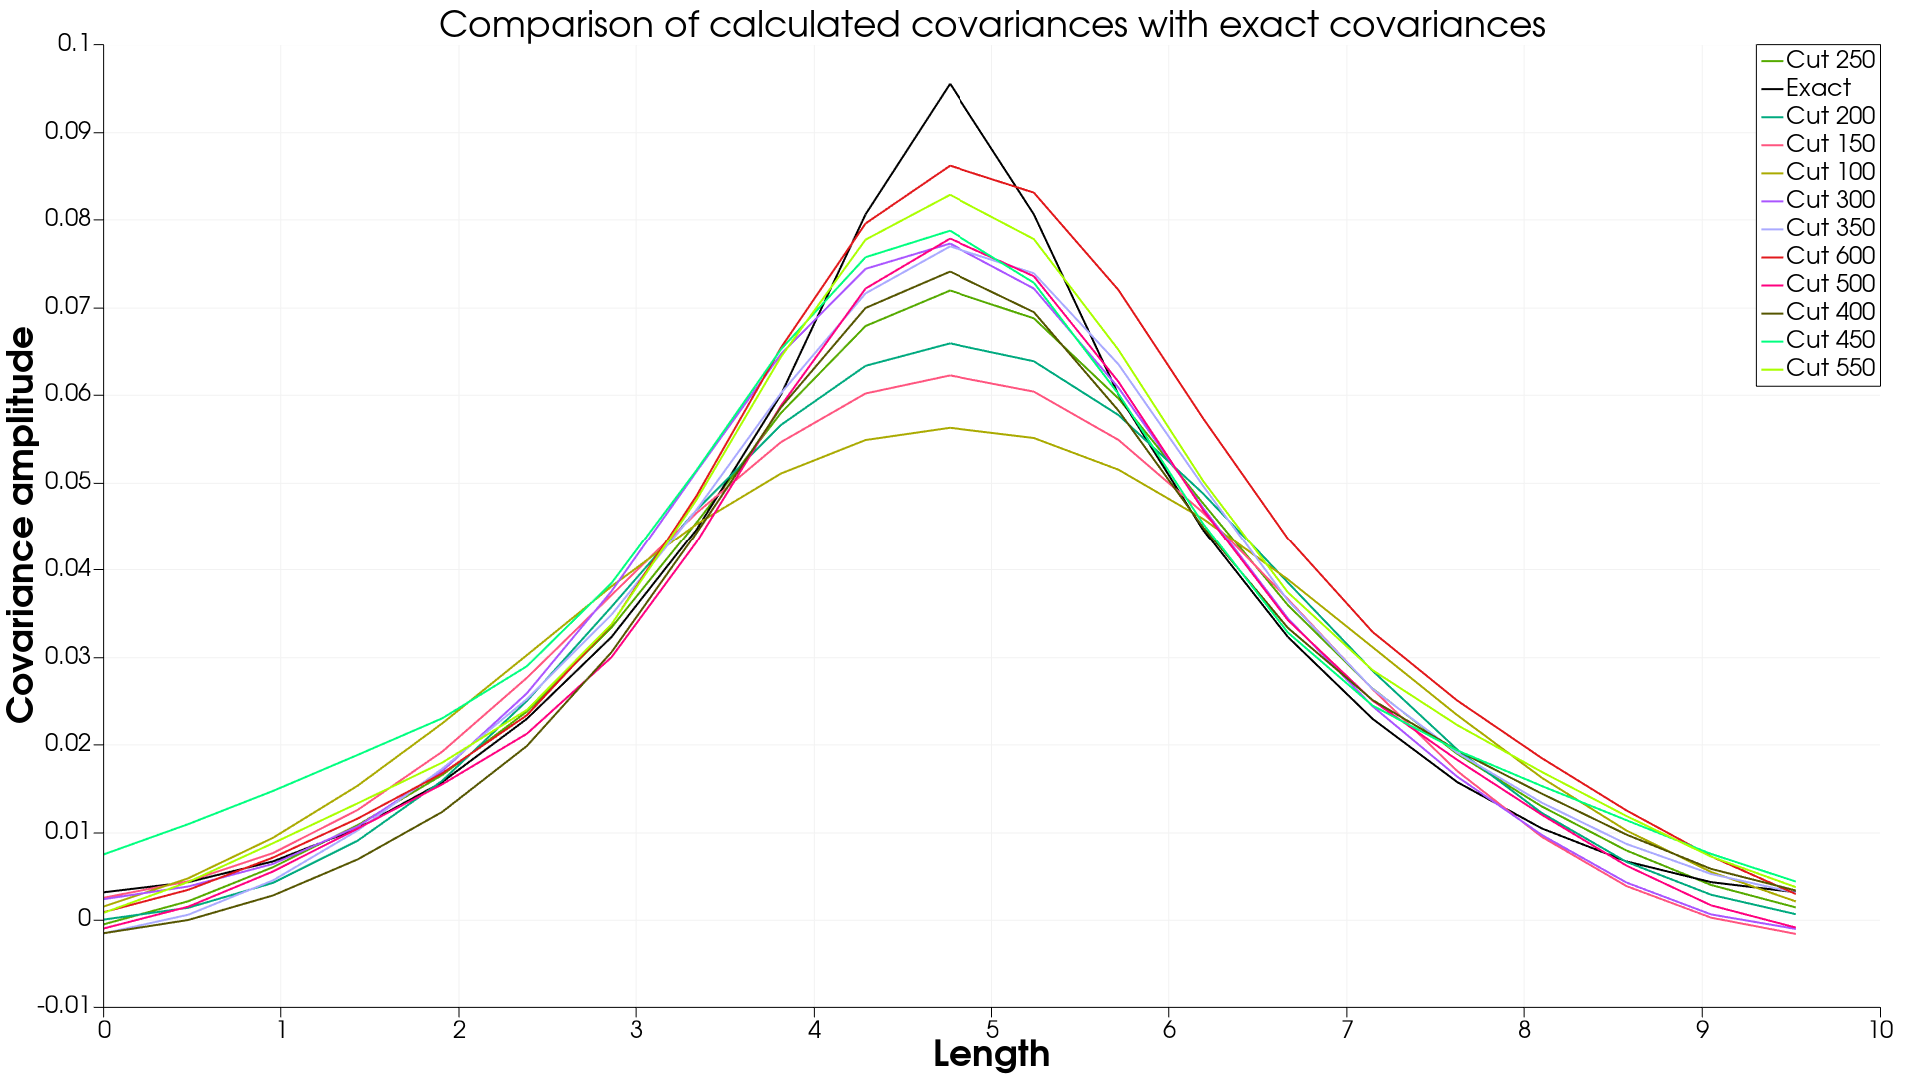
\includegraphics[width=0.4\linewidth]{comparison_covcut4_x}} \\
        \hfill
        \subcaptionbox[List-of-Figures entry]{$y$ направление\label{img:comparison_covcut4_y}} 
        {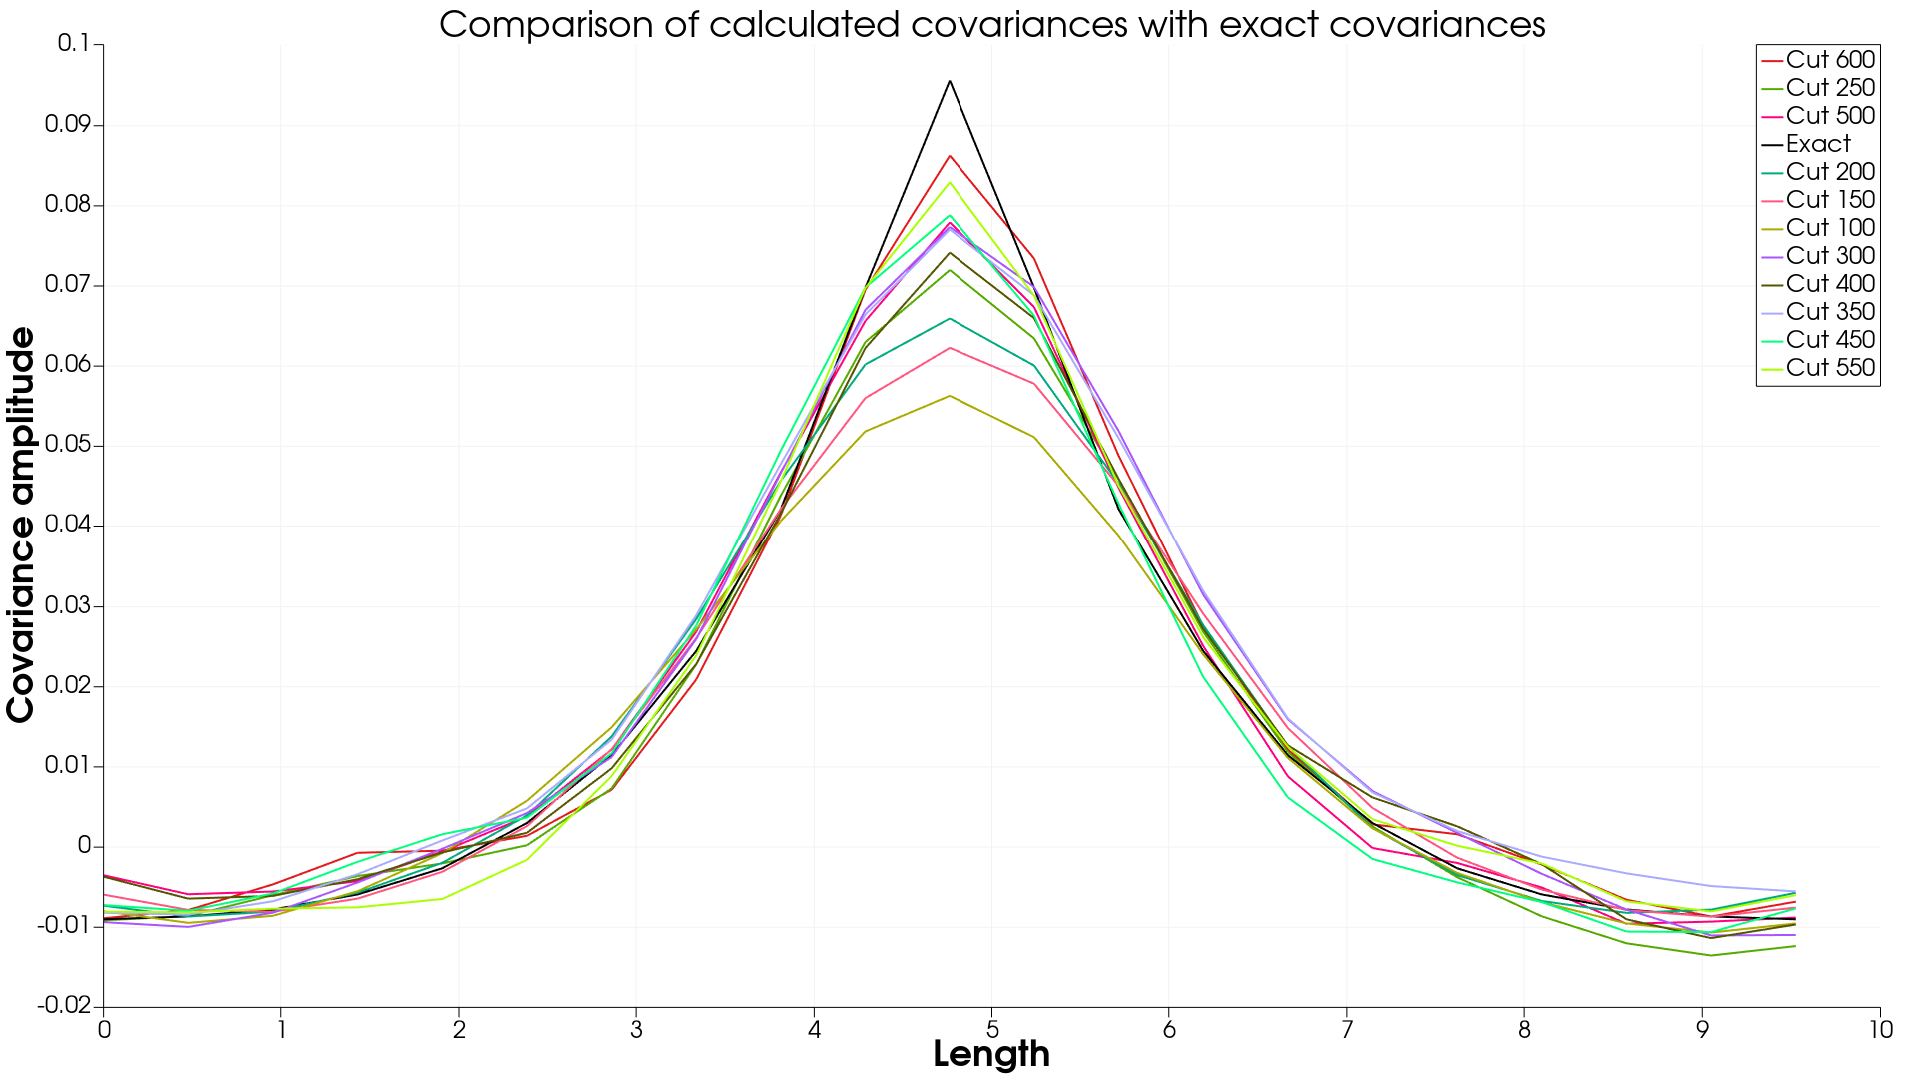
\includegraphics[width=0.4\linewidth]{comparison_covcut4_y}}%
        \hfill       
        \subcaptionbox{$z$ направление\label{img:comparison_covcut4_z}} 
        {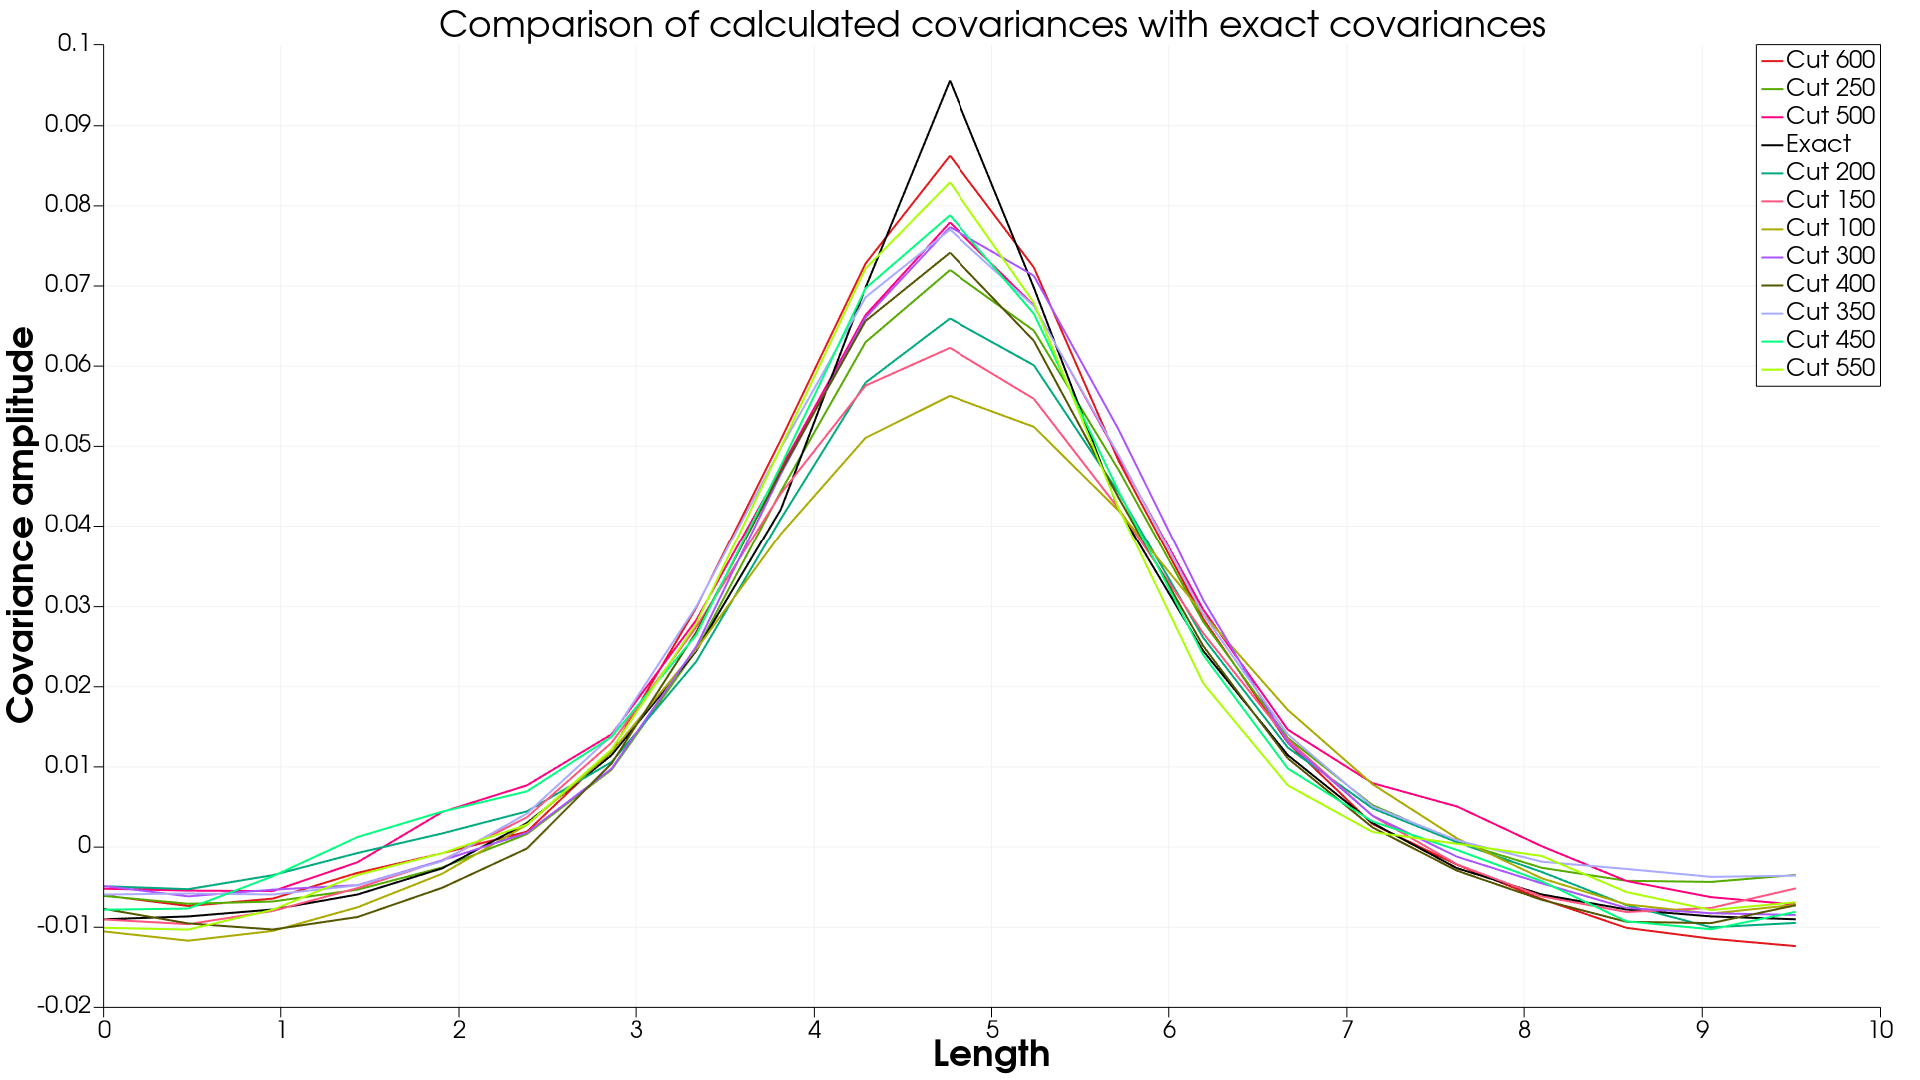
\includegraphics[width=0.4\linewidth]{comparison_covcut4_z}}
        \hfill
    }
    
    \onehalfspacing{Сравнение ковариацинной функции, допуск 4\%, для направлений а) вдоль диагонали, б) вдоль оси $x$, в) вдоль оси $y$, г) вдоль оси $z$}
    \caption{Сравнение ковариационной функции для допуска по амплитуде ковариаций в 4\% для различных направлений в рассматриваемой области}
    \label{img:covcut_4_comparison}  
\end{figure}
%
% Обрезание 5%
%
\begin{figure}[!h]
    \center{
        \hfill
        \subcaptionbox[List-of-Figures entry]{диагональ\label{img:comparison_covcut5_diag}} 
        {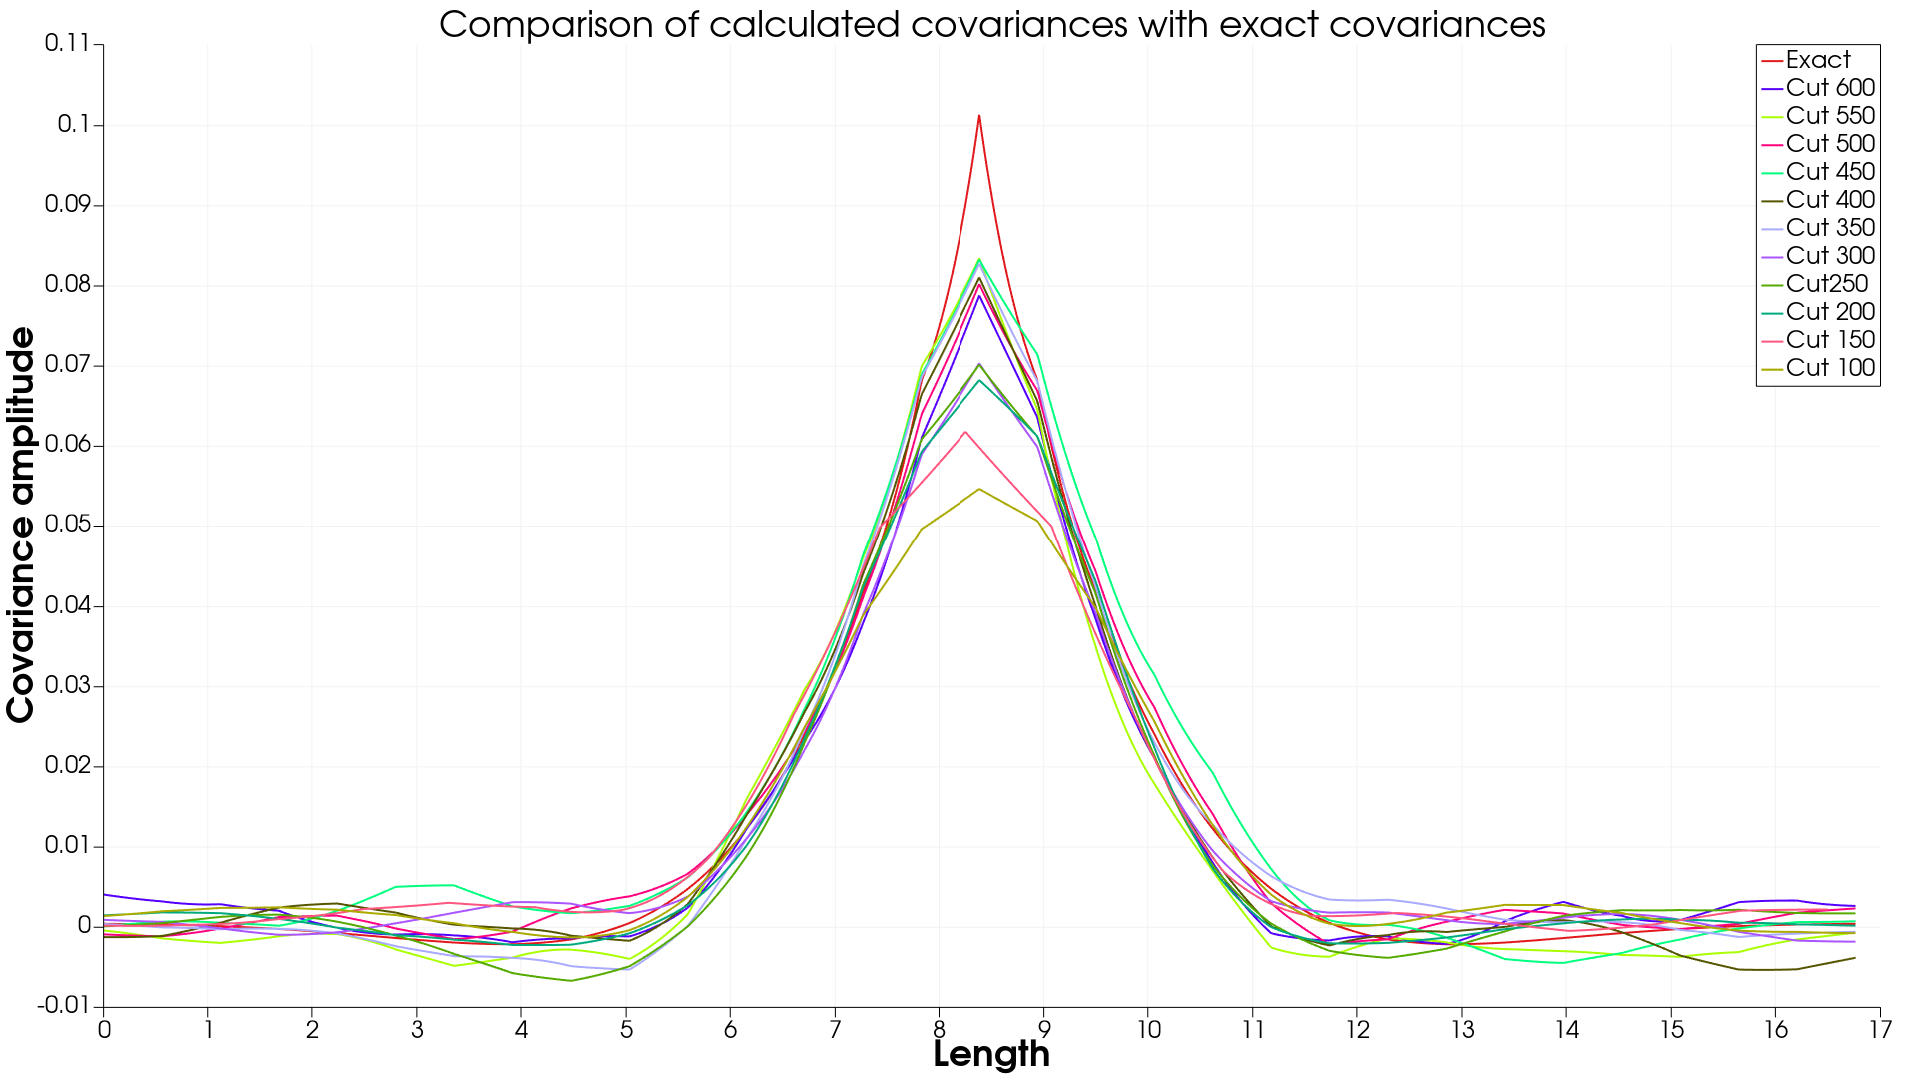
\includegraphics[width=0.4\linewidth]{comparison_covcut5_diag}}%
        \hfill       
        \subcaptionbox{$x$ направление\label{img:comparison_covcut5_x}} 
        {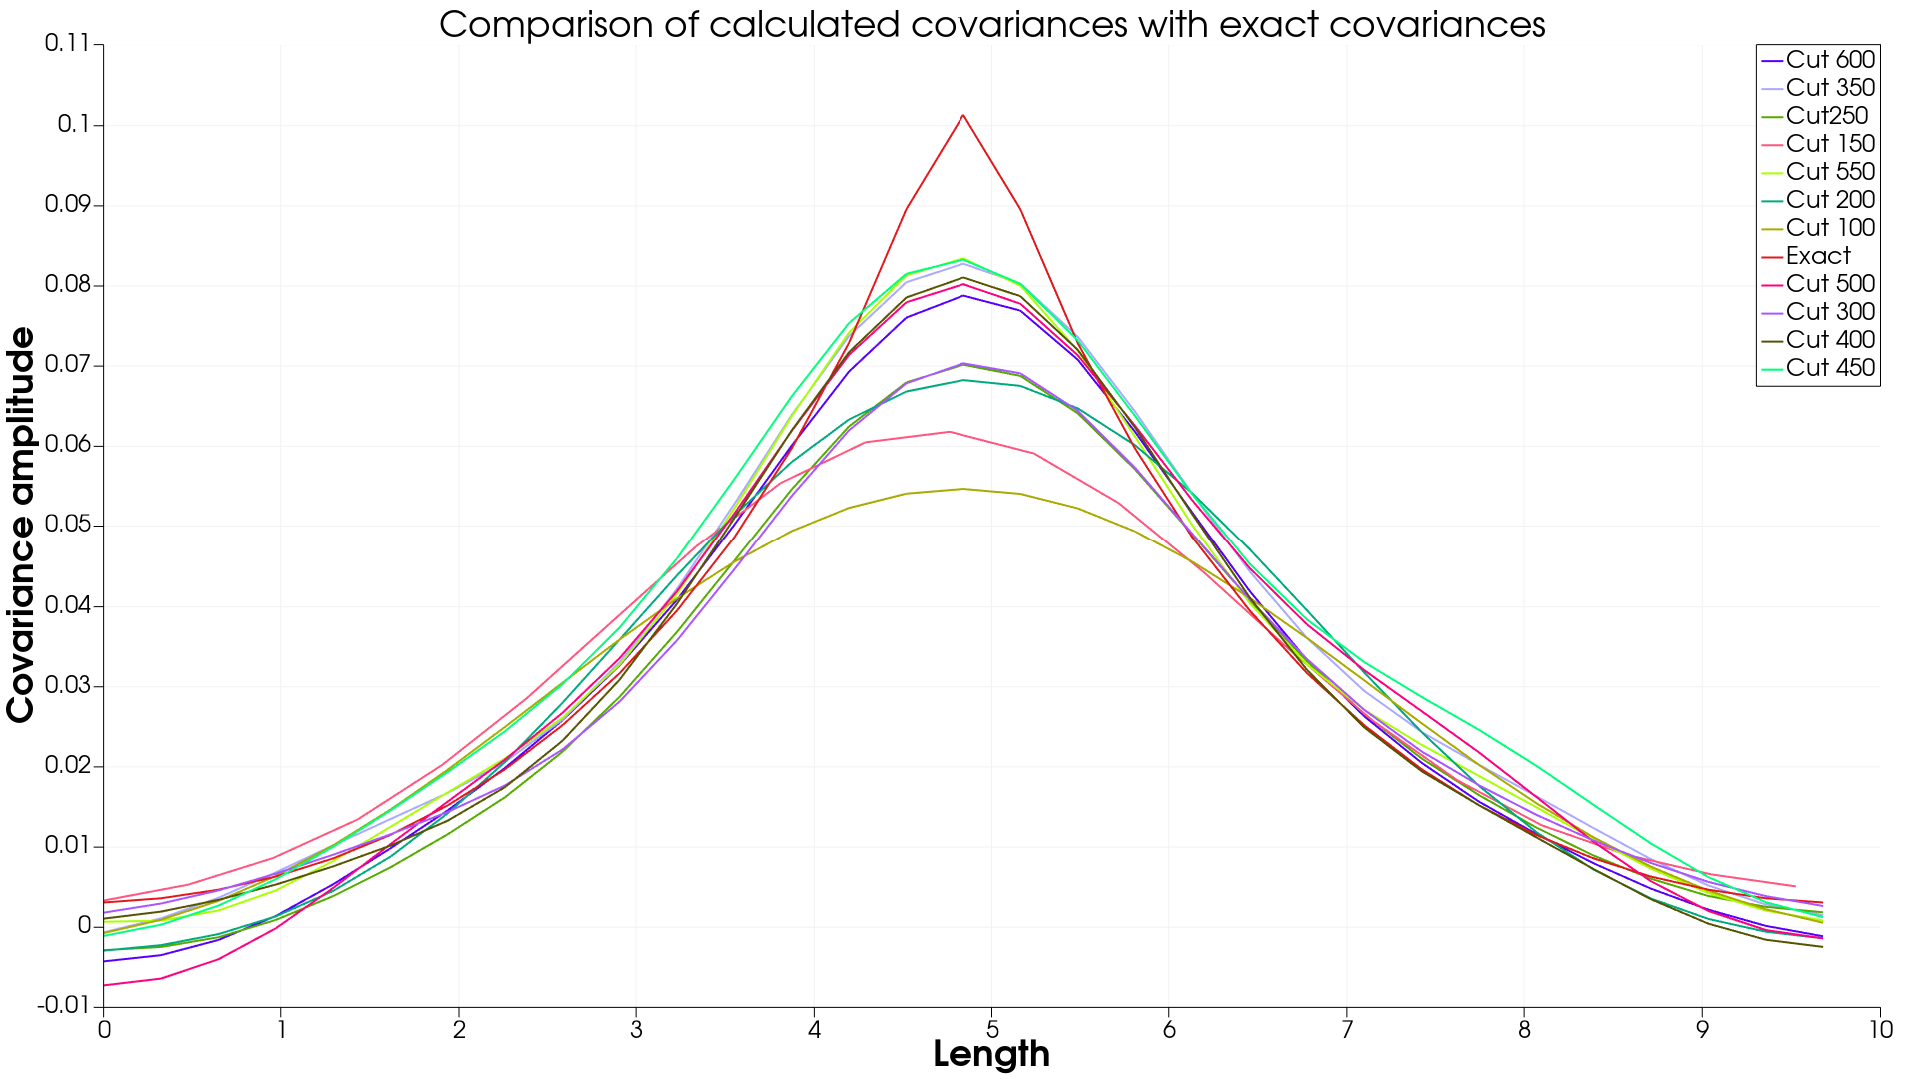
\includegraphics[width=0.4\linewidth]{comparison_covcut5_x}} \\
        \hfill
        \subcaptionbox[List-of-Figures entry]{$y$ направление\label{img:comparison_covcut5_y}} 
        {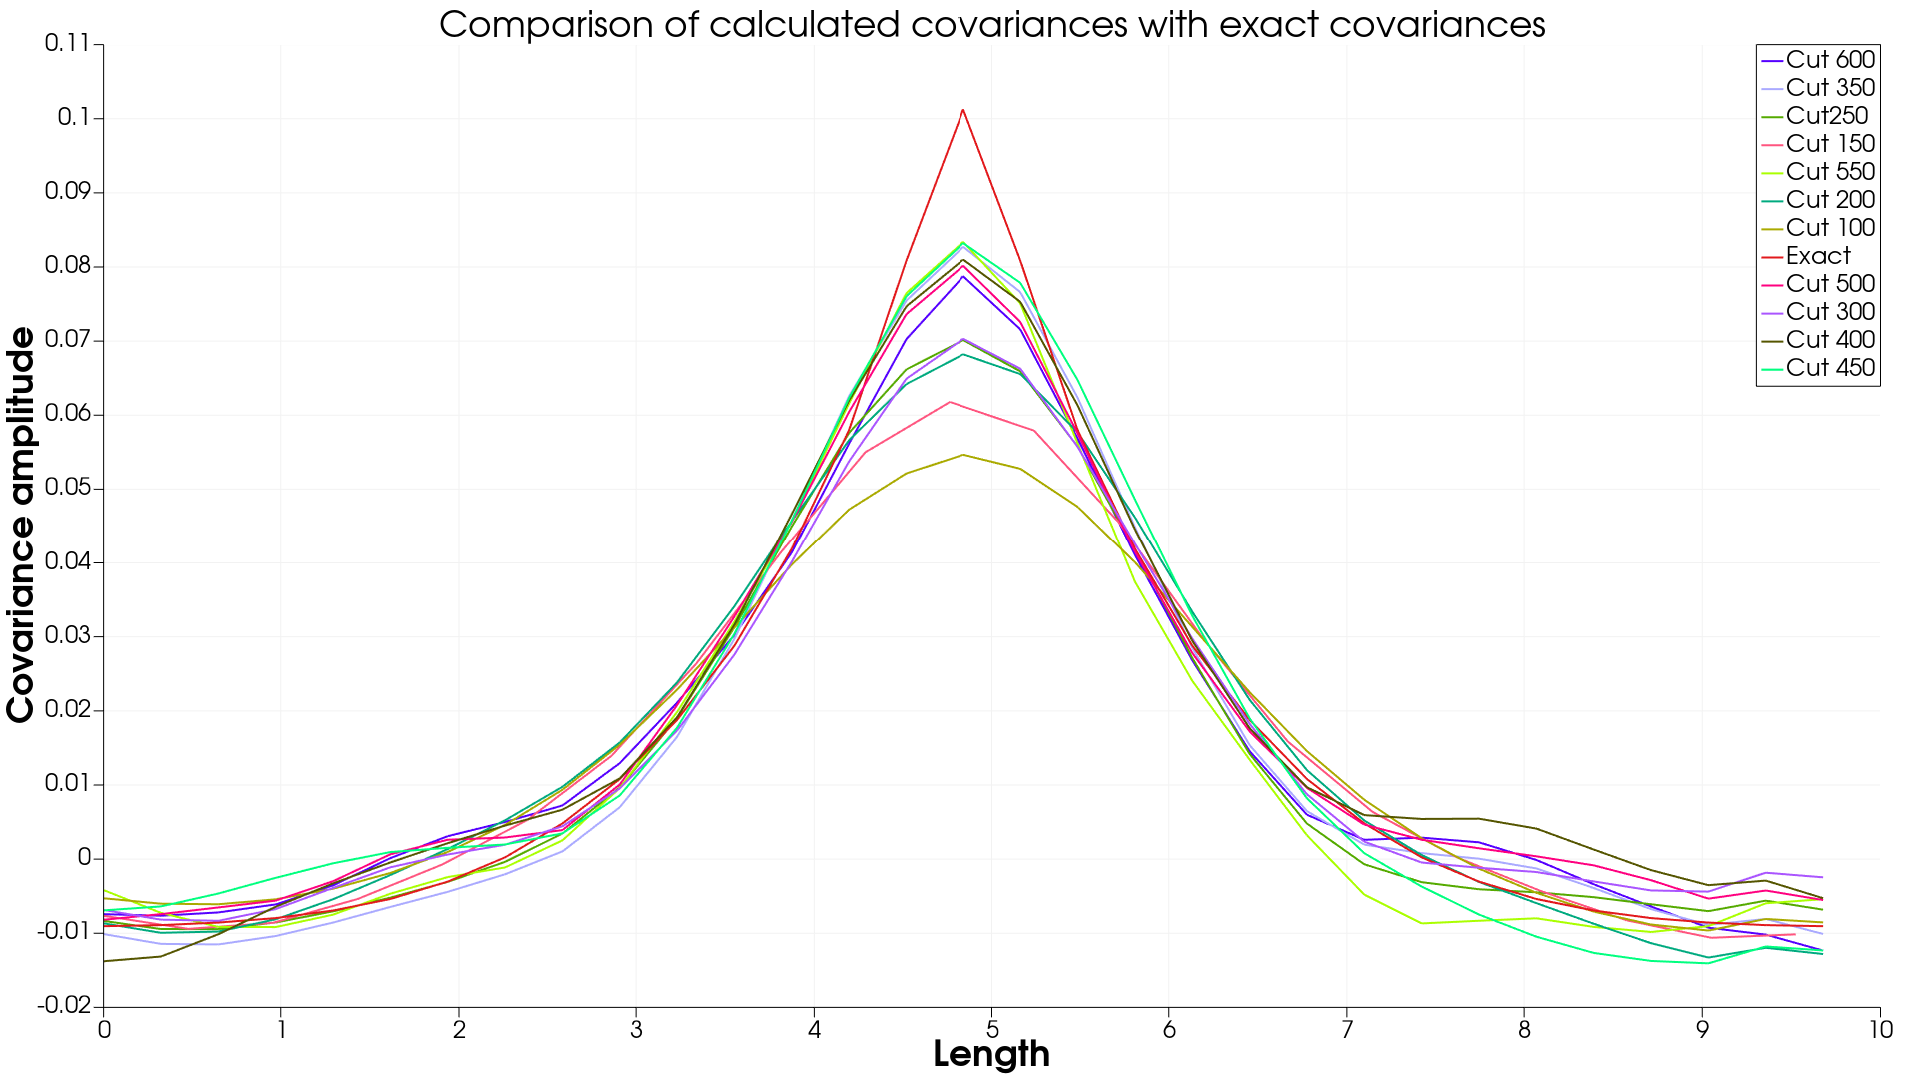
\includegraphics[width=0.4\linewidth]{comparison_covcut5_y}}%
        \hfill       
        \subcaptionbox{$z$ направление\label{img:comparison_covcut5_z}} 
        {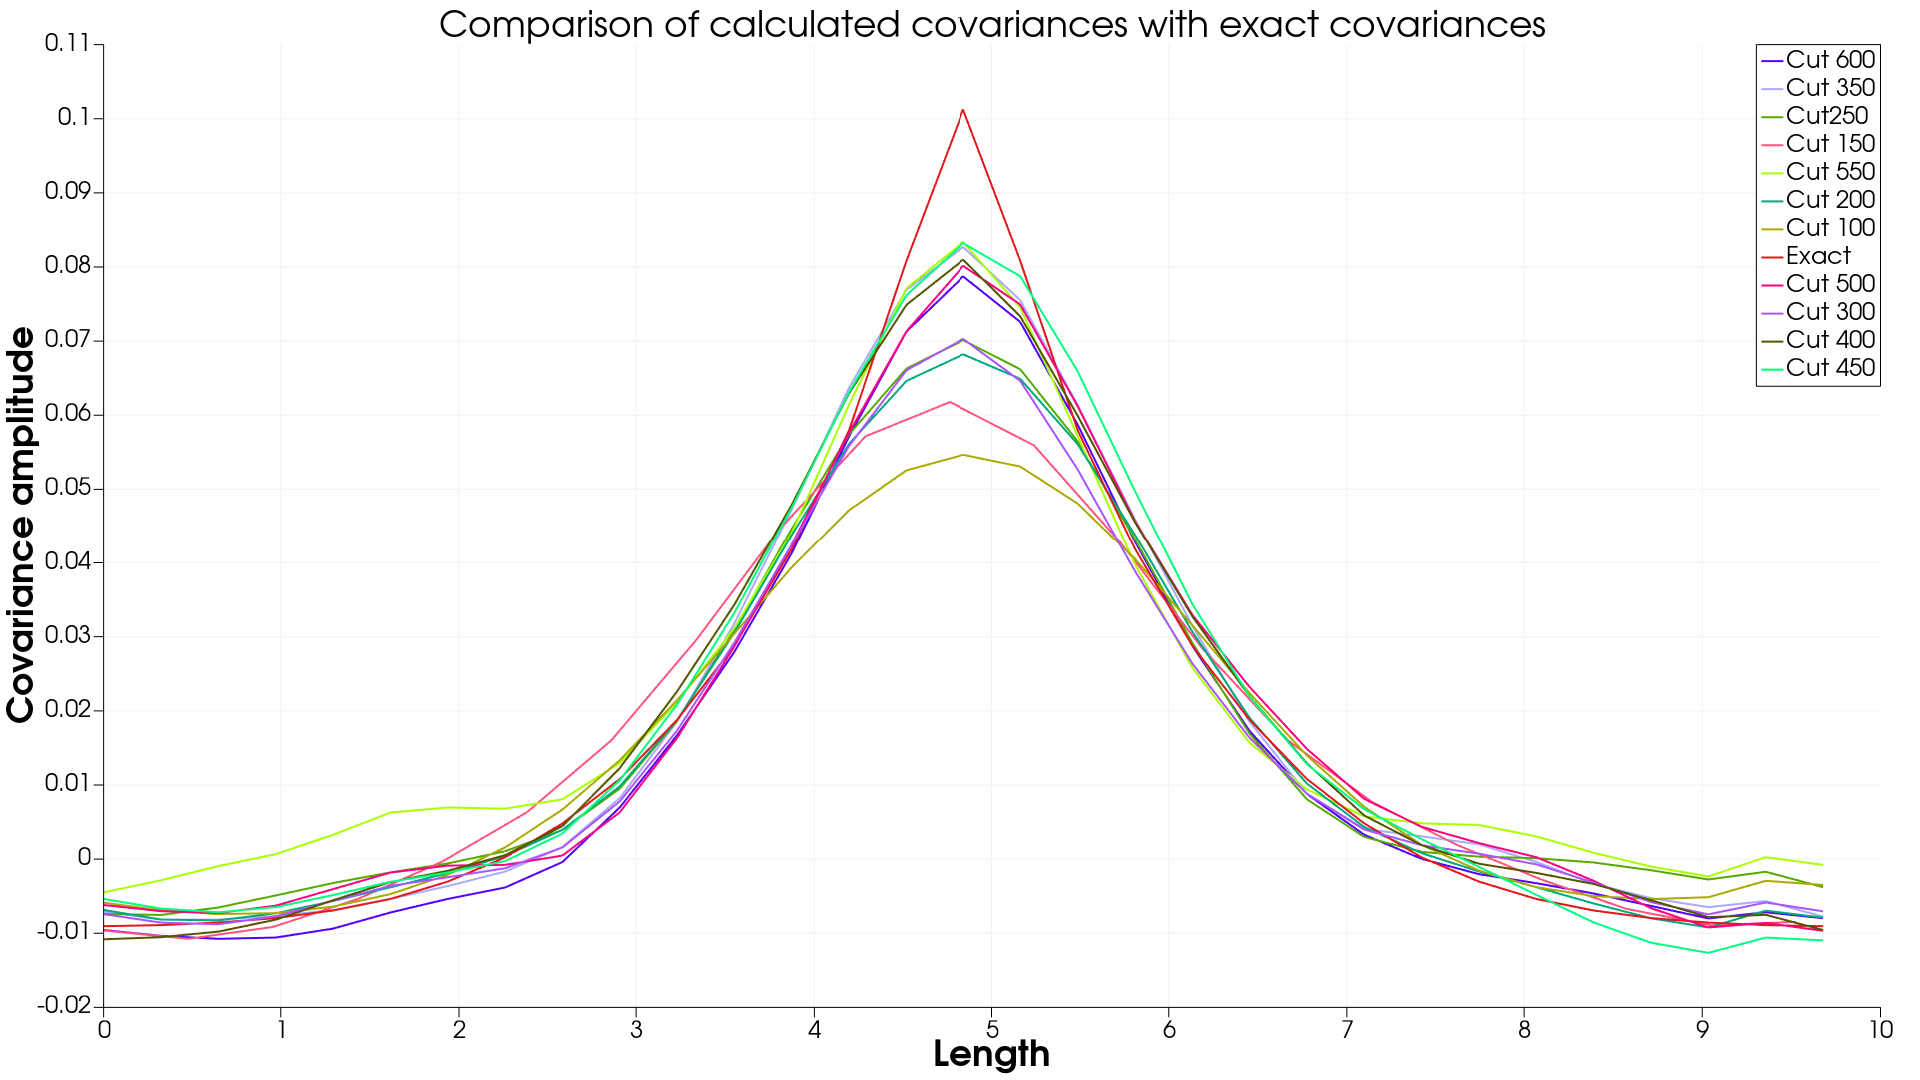
\includegraphics[width=0.4\linewidth]{comparison_covcut5_z}}
        \hfill
    }
    
    \onehalfspacing{Сравнение ковариацинной функции, допуск 5\%, для направлений а) вдоль диагонали, б) вдоль оси $x$, в) вдоль оси $y$, г) вдоль оси $z$}
    \caption{Сравнение ковариационной функции для допуска по амплитуде ковариаций в 5\% для различных направлений в рассматриваемой области}
    \label{img:covcut_5_comparison}  
\end{figure}

Так как расчёт статистических параметров, например ковариационной функции, требует какого-то набора реализаций полей скорости, необходимо также проверить, как влияет число генерируемых полей для подсчёта статистических характеристик. Это важный критерий в силу того, что основными параметрами валидации являются статистические величины. Естественно, наиболее точный случай это бесконечное число реализаций, но это также несёт в себе дополнительные временные затраты. Например, если необходимо для случая генерации поля на некоторой сетке оценить то, как хорошо метод подходит для использования на данной топологии сетки, или, например, какое число собственных значений и векторов стоит брать для последующей генерации флуктуации необходимо провести статистическое исследование, дабы не увеличивать требуемое время, стоит провести оценку некоторого оптимального числа реализаций, на котором можно проводить последующие валидации. На рисунке \ref{covcut0_eigvalues_step_samples} ниже представлены сравнение ковариационных функций, полученных в результате использования $n$ реализаций поля скоростей для подсчёта. В целом, для числа реализаций равного 1000, уже наблюдается хорошее совпадение с целевым спектром вблизи его пика, чем дальше мы отдаляемся от центра куба, тем сильнее начинает играть роль число взятых сгенерированных полей. С ростом числа взятых для расчёта реализаций также уменьшается разница между целевой ковариационной функций и рассчитанной.

\begin{figure}[!h]
    \center{
        \hfill
        \subcaptionbox[List-of-Figures entry]{диагональ\label{img:diagonal_alleigenvalues_samples_step}} 
        {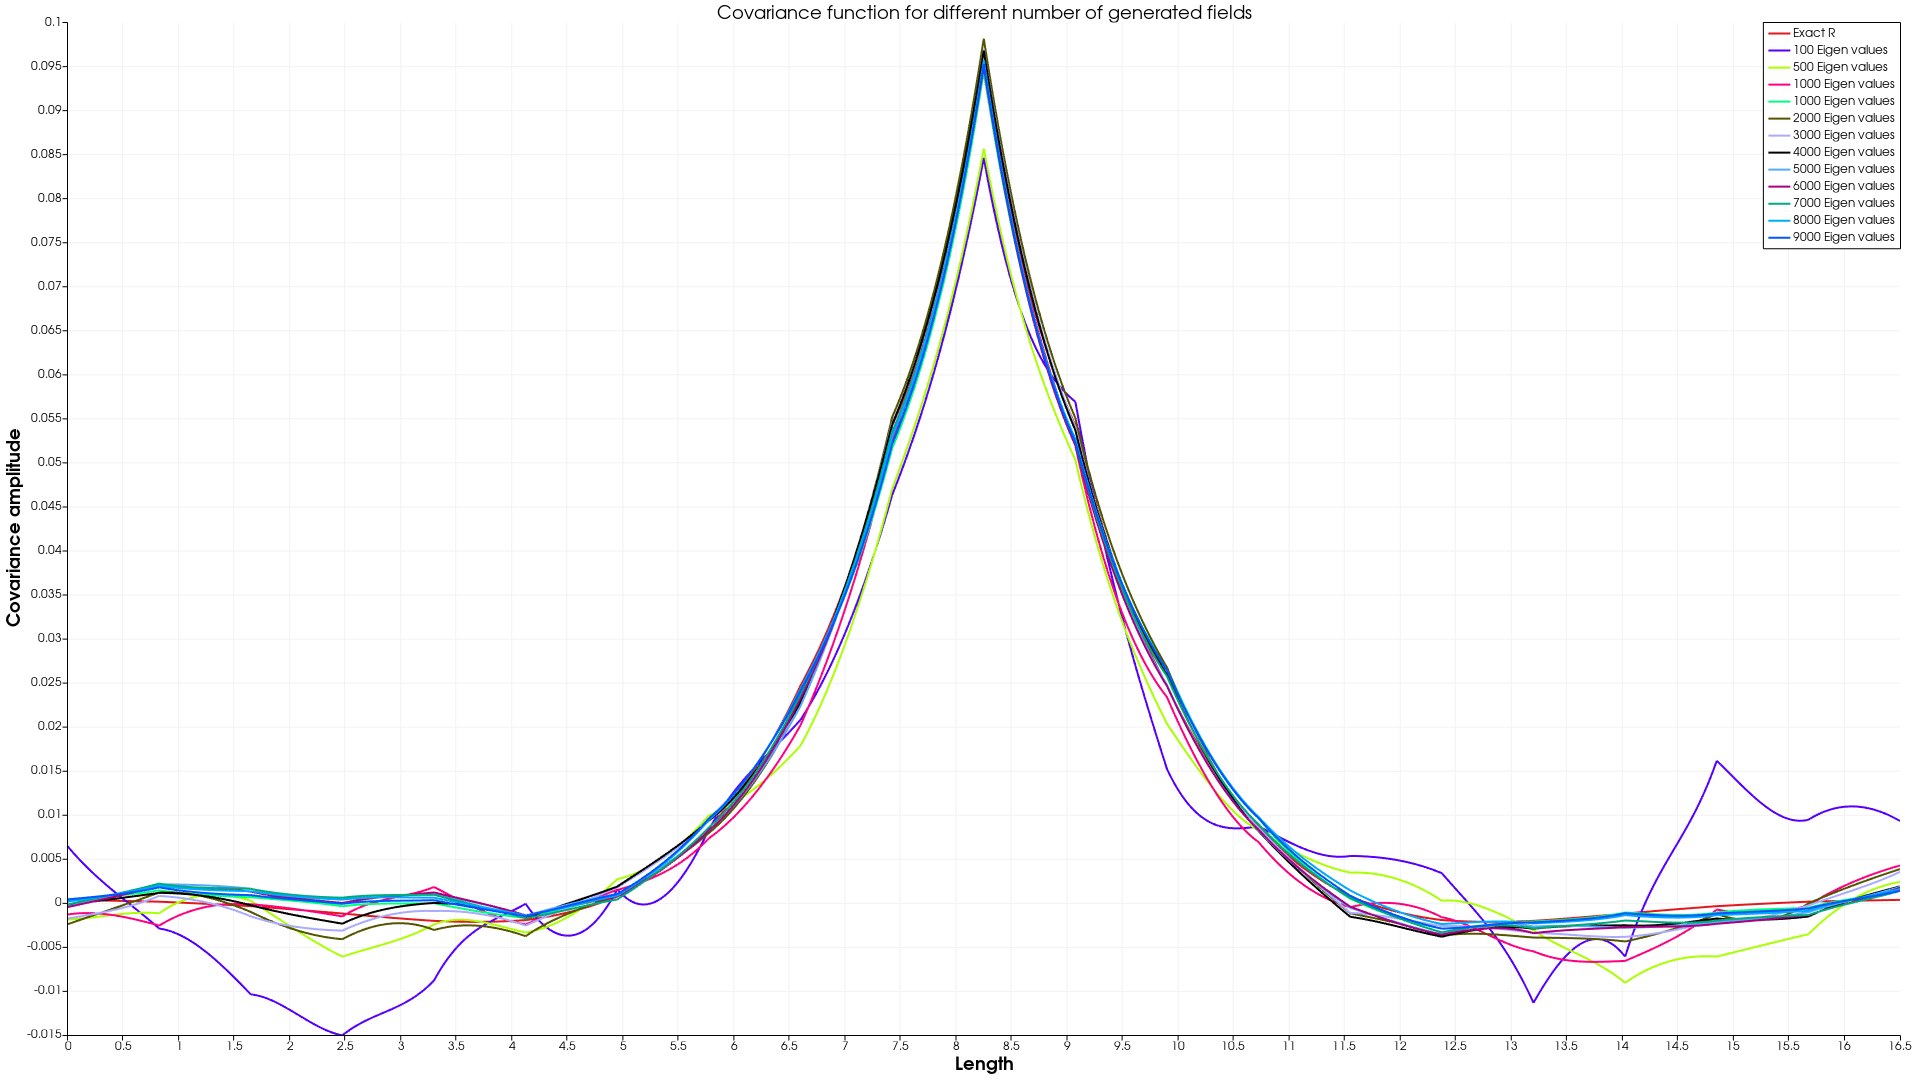
\includegraphics[width=0.4\linewidth]{diagonal_alleigenvalues_samples_step}}%
        \hfill       
        \subcaptionbox{$x$ направление\label{img:x_axis_alleigenvalues_samples_step}} 
        {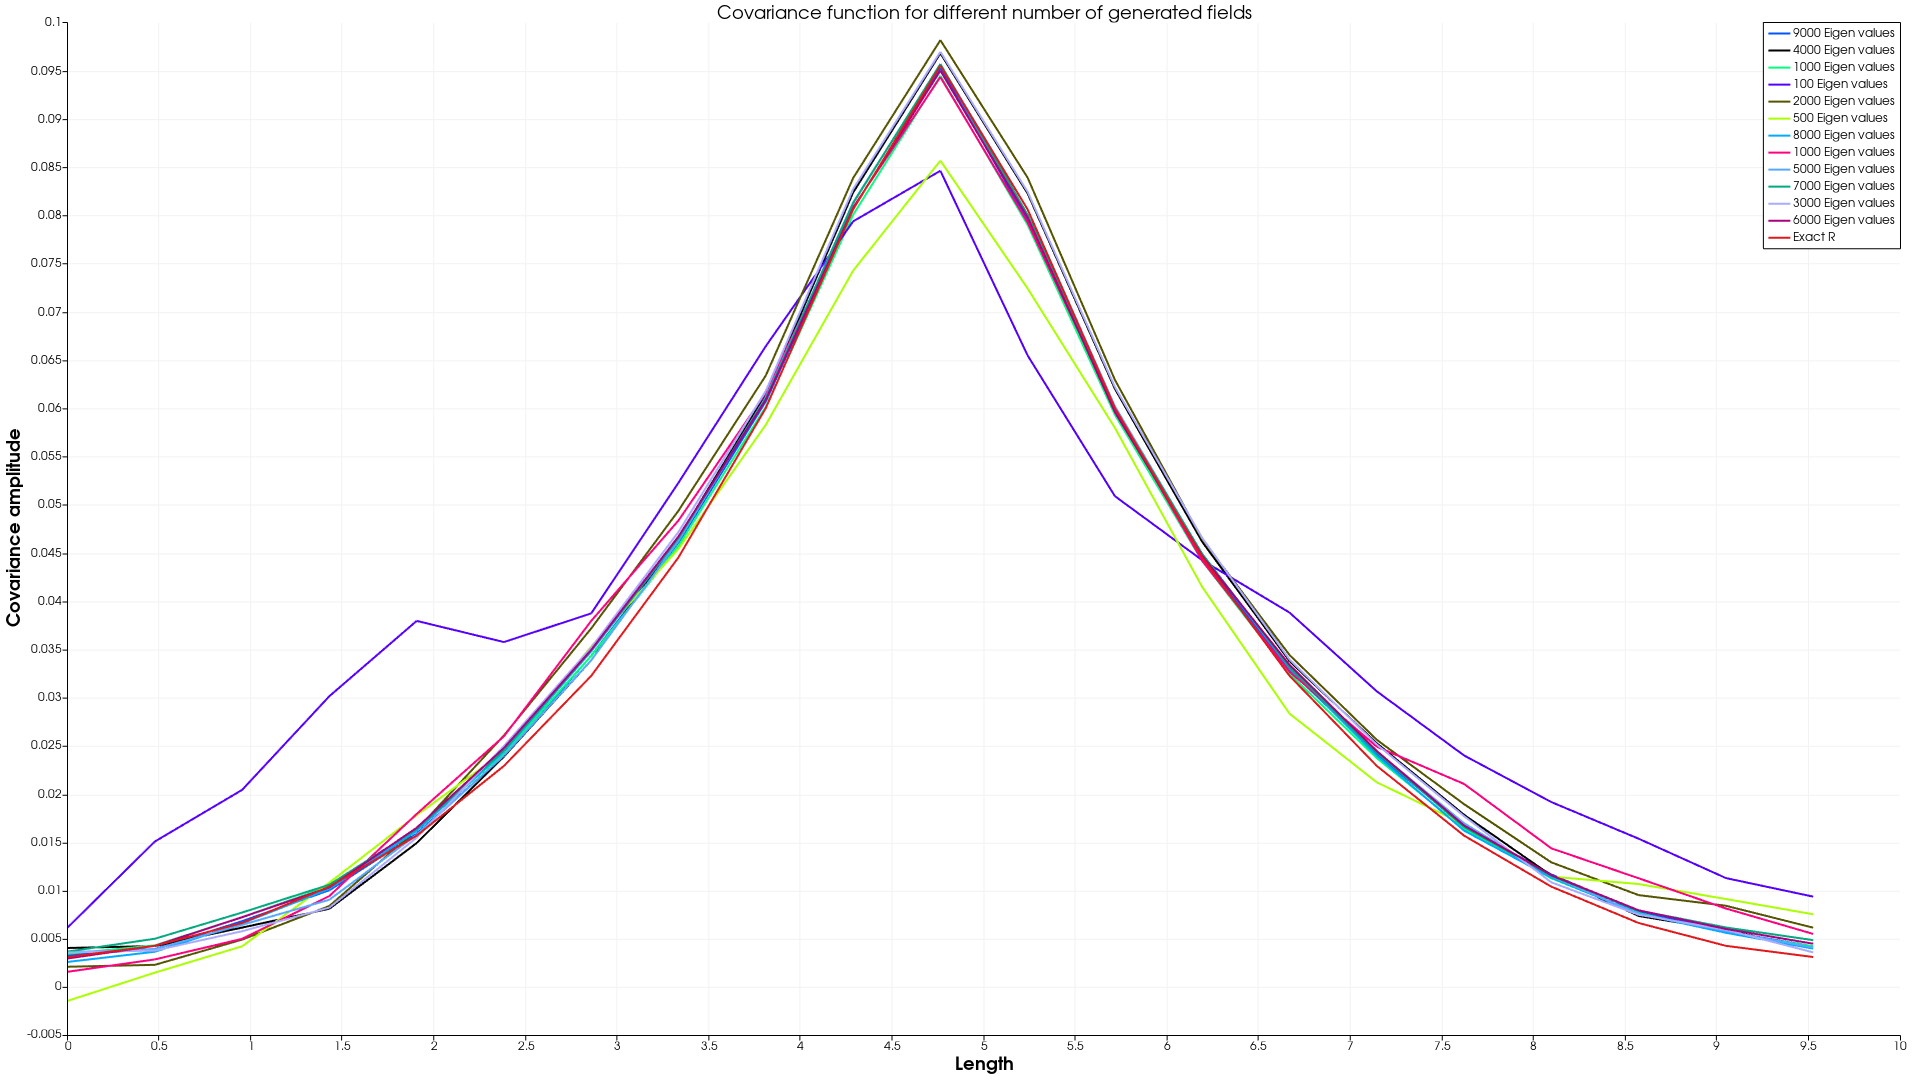
\includegraphics[width=0.4\linewidth]{x_axis_alleigenvalues_samples_step}} \\
        \hfill
        \subcaptionbox[List-of-Figures entry]{$y$ направление\label{img:y_axis_alleigenvalues_samples_step}} 
        {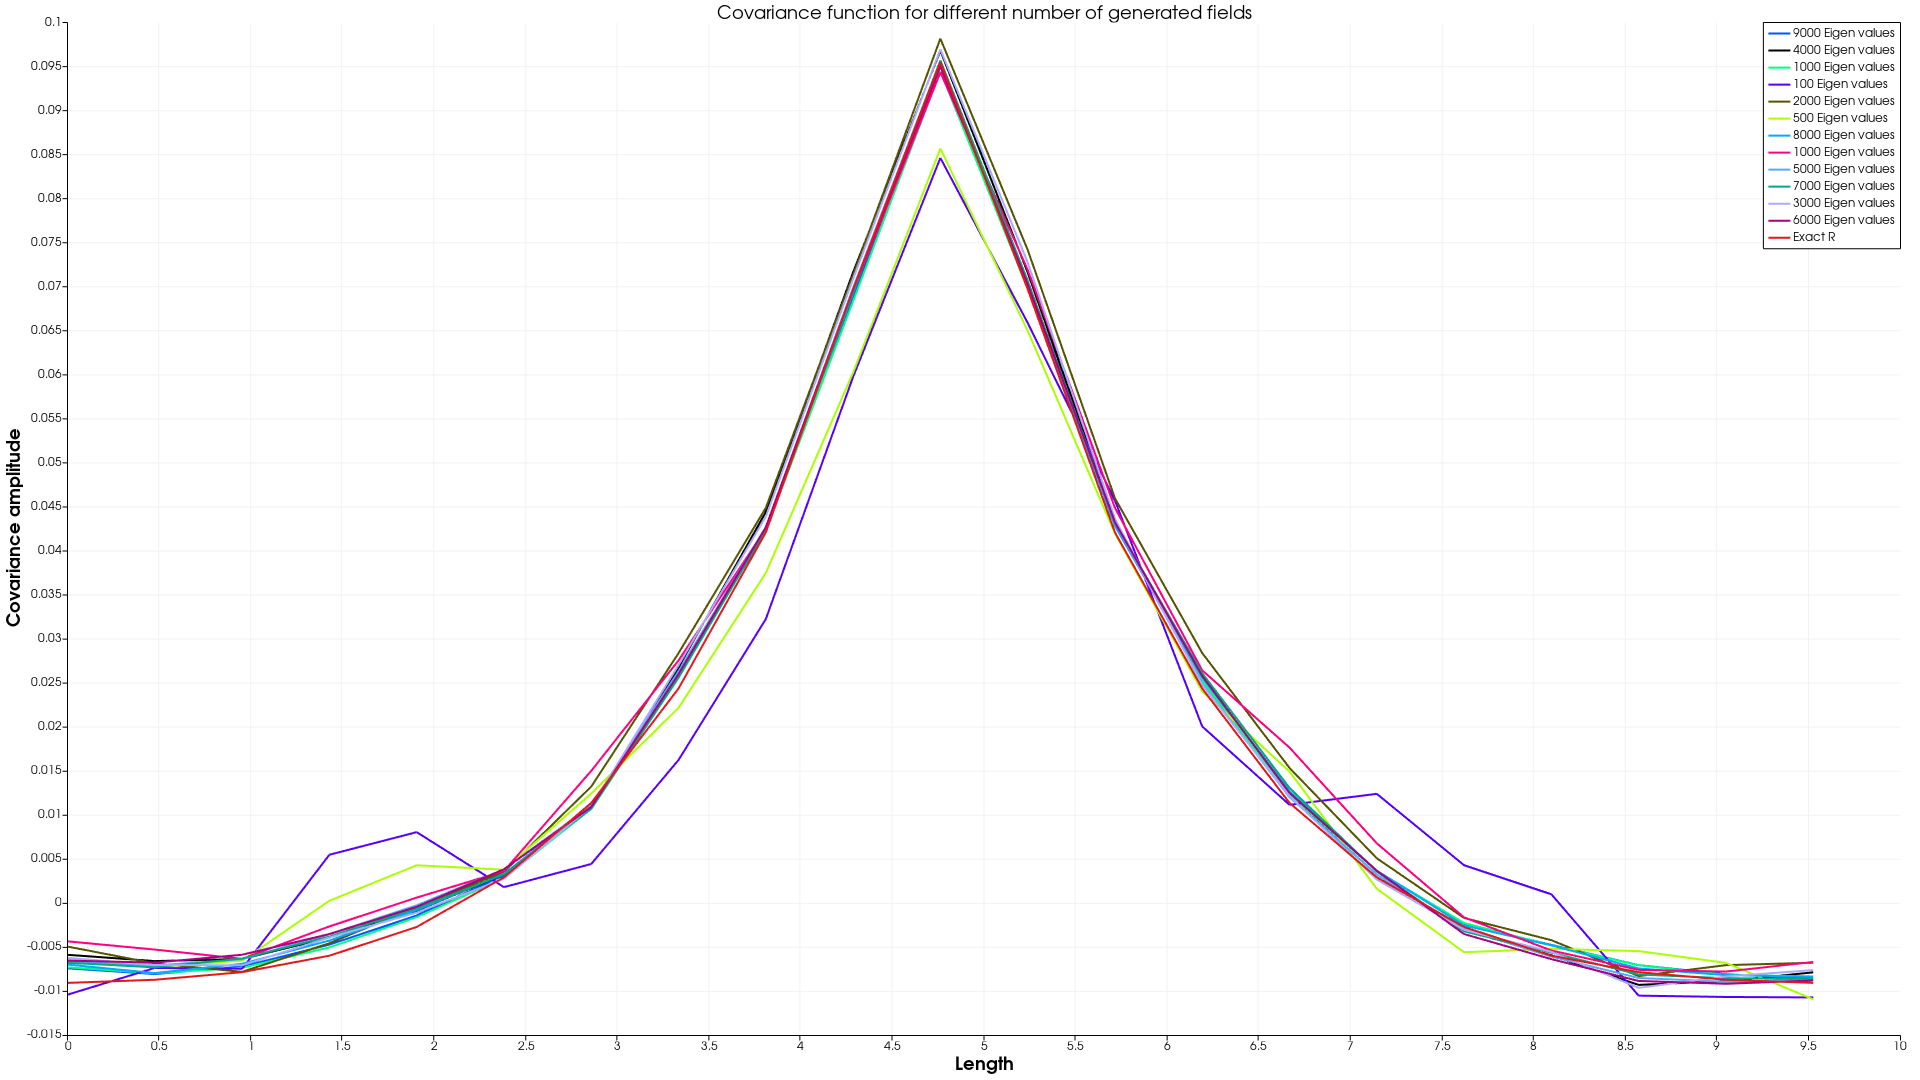
\includegraphics[width=0.4\linewidth]{y_axis_alleigenvalues_samples_step}}%
        \hfill       
        \subcaptionbox{$z$ направление\label{img:z_axis_alleigenvalues_samples_step}} 
        {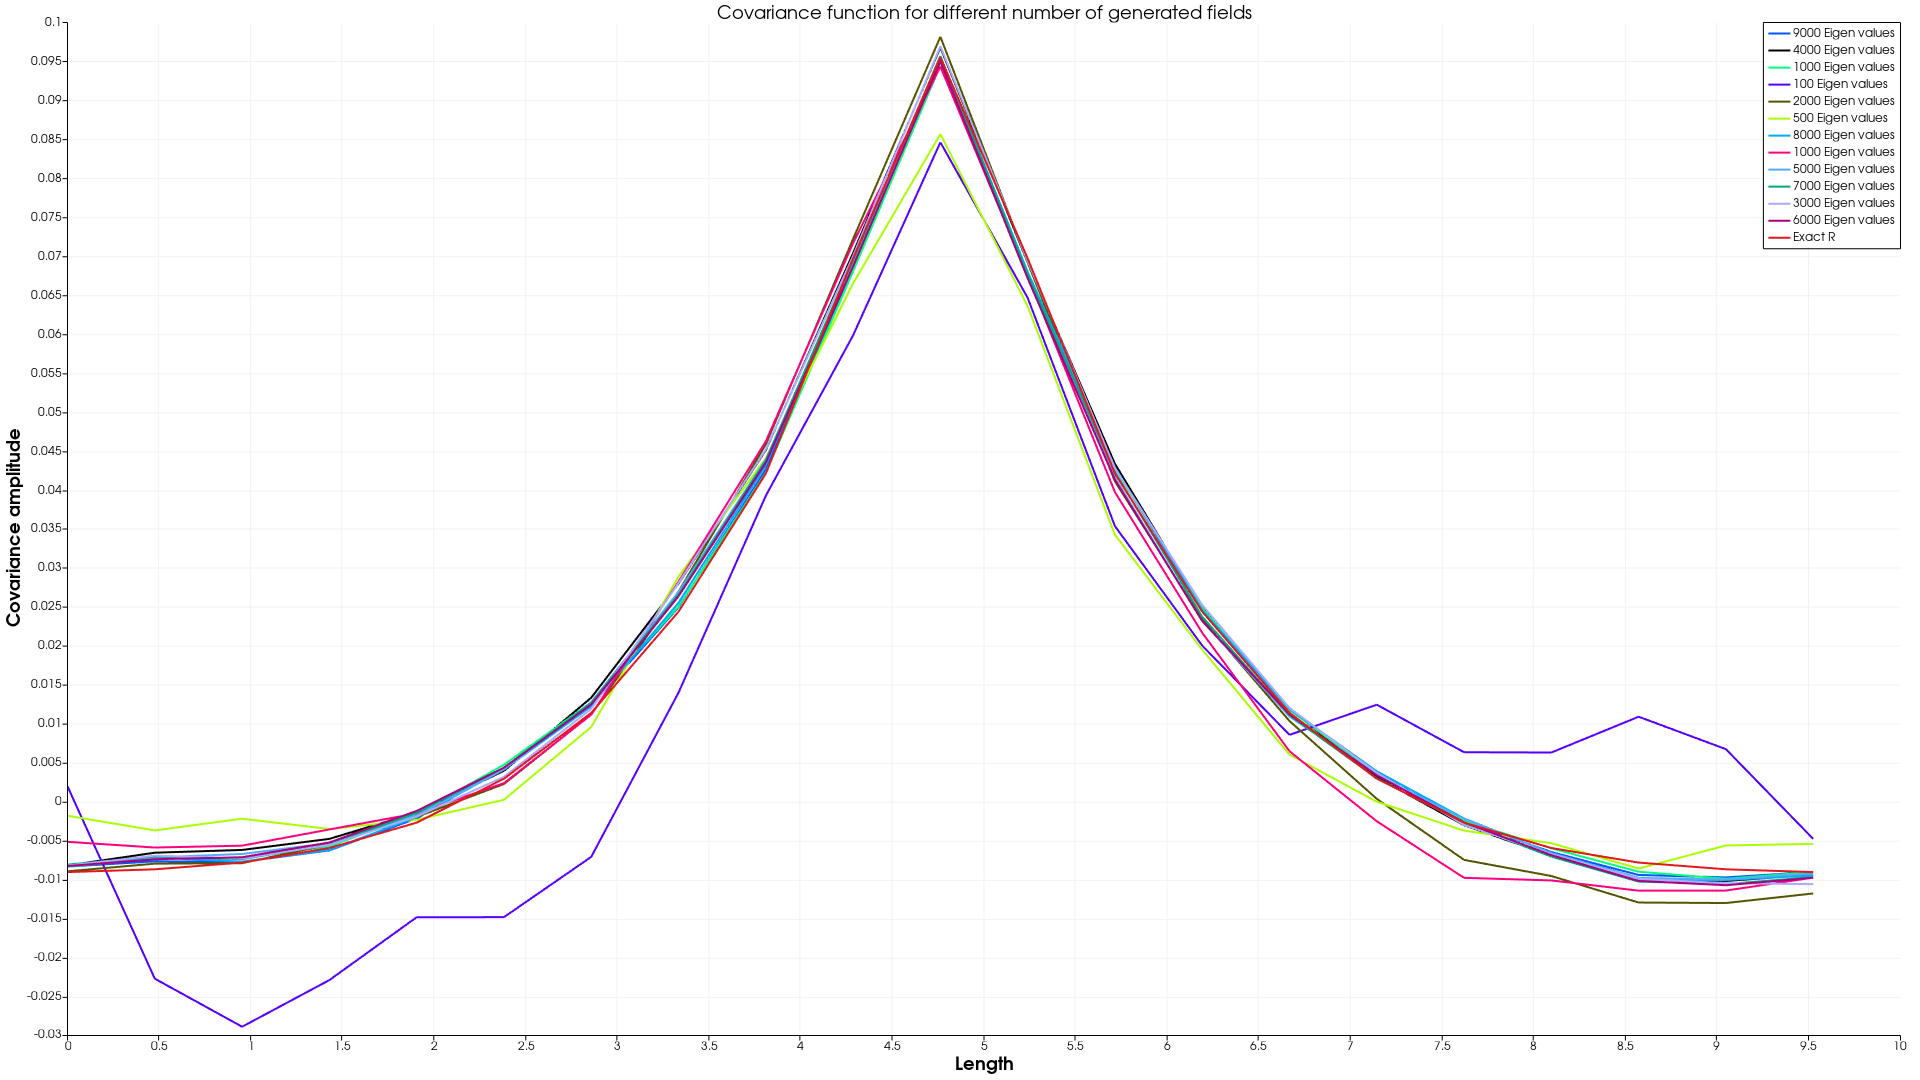
\includegraphics[width=0.4\linewidth]{z_axis_alleigenvalues_samples_step}}
        \hfill
    }
    
    \onehalfspacing{Сравнение ковариацинной функции, допуск 0\%, для направлений а) вдоль диагонали, б) вдоль оси $x$, в) вдоль оси $y$, г) вдоль оси $z$}
    \caption{Сравнение ковариационной функции для допуска по амплитуде ковариаций в 0\% для различного числа взятых реализаций полей флуктуаций для расчёта ковариационной функции в рассматриваемой области}
    \label{img:covcut0_eigvalues_step_samples}  
\end{figure}

\begin{table} [!h]%
	\caption{Величина разности между пиками для смоделированных ковариационных функций с пиком полученным из аналитического спектра преобразованием Фурье}%
	\label{tbl:peak_diff_table}
    \setlength\extrarowheight{4pt} %вот этим управляем расстоянием между рядами, \arraystretch даёт неудачный результат
    \setlength{\tymin}{1.5cm}
\begin{tabulary}{\textwidth}{@{}>{\zz}L >{\zz}C >{\zz}C >{\zz}C >{\zz}C >{\zz}C >{\zz}C@{}}
        \toprule     %%% верхняя линейка
            Число собственных значений &
            Допуск 0\% &
    	Допуск 1\% &
    	Допуск 2\% &
            Допуск 3\% &
            Допуск 4\% &
            Допуск 5\% \\
        \midrule %%% тонкий разделитель. Отделяет названия столбцов. Обязателен по ГОСТ 2.105 пункт 4.4.5 
        100 & -0.03868 & -0.04020 & -0.03814 & -0.03944  & -0.03927  & -0.0466  \\
        150 & -0.03188 & -0.03672 & -0.03047 & -0.03574  & -0.03329  & -0.03375 \\
        200 & -0.03150 & -0.02799 & -0.02830 & -0.02918  & -0.02963  & -0.03303 \\
        250 & -0.02461 & -0.02697 & -0.02748 & -0.03013  & -0.02360  & -0.03111 \\
        300 & -0.02429 & -0.02242 & -0.02693 & -0.02630  & -0.01824  & -0.03094 \\
        350 & -0.02210 & -0.02132 & -0.02638 & -0.02462  & -0.01856  & -0.01853 \\
        400 & -0.03234 & -0.01948 & -0.02341 & -0.02631  & -0.02144  & -0.02025 \\
        450 & -0.02727 & -0.02309 & -0.01800 & -0.007552 & -0.01678  & -0.01803 \\
        500 & -0.02283 & -0.02383 & -0.02184 & -0.01308  & -0.01767  & -0.02109 \\
        550 & -0.02075 & -0.02574 & -0.01990 & -0.01961  & -0.01268  & -0.01786 \\
        600 & -0.01870 & -0.01512 & -0.01590 & -0.01079  & -0.009351 & -0.02251 \\
        \midrule%%% тонкий разделитель
        \multicolumn{7}{@{}p{\textwidth}}{%
            \vspace*{-4ex}% этим подтягиваем повыше
            \hspace*{2.5em}% абзацный отступ - требование ГОСТ 2.105
            Примечание -- значения заданы до 4 значащих цифр
        }
        \\
        \bottomrule %%% нижняя линейка
    \end{tabulary}%
\end{table}

В таблице \ref{peak_diff_table} представлены значения разности между пиком точной функции и пиками для функций отвечающим различному числу взятых собственных чисел. 

\begin{table} [!h]%
	\caption{Величина $\iiint_V (R - R_{exact})^2 dV$ смоделированных ковариационных функций с пиком полученным из аналитического спектра преобразованием Фурье}%
	\label{tbl:sqr_diff_table}
    \setlength\extrarowheight{4pt} %вот этим управляем расстоянием между рядами, \arraystretch даёт неудачный результат
    \setlength{\tymin}{1.5cm}
\begin{tabulary}{\textwidth}{@{}>{\zz}L >{\zz}C >{\zz}C >{\zz}C >{\zz}C >{\zz}C >{\zz}C@{}}
        \toprule     %%% верхняя линейка
            Число собственных значений &
            Допуск 0\% &
    	Допуск 1\% &
    	Допуск 2\% &
            Допуск 3\% &
            Допуск 4\% &
            Допуск 5\% \\
        \midrule %%% тонкий разделитель. Отделяет названия столбцов. Обязателен по ГОСТ 2.105 пункт 4.4.5 
        100 & 0.005392 & 0.005629 & 0.005147 & 0.005709  & 0.005091  & 0.005871  \\
        150 & 0.004312 & 0.004123 & 0.004802 & 0.004546  & 0.004971  & 0.005351 \\
        200 & 0.004390 & 0.004272 & 0.003796 & 0.005035  & 0.005468  & 0.007215 \\
        250 & 0.004358 & 0.003895 & 0.004723 & 0.004545  & 0.006956  & 0.007789 \\
        300 & 0.004783 & 0.005905 & 0.004314 & 0.005086  & 0.006408  & 0.007328 \\
        350 & 0.005015 & 0.005662 & 0.005505 & 0.005314  & 0.007291  & 0.008133 \\
        400 & 0.005787 & 0.006087 & 0.005244 & 0.004887  & 0.006656  & 0.01095 \\
        450 & 0.005369 & 0.004789 & 0.005936 & 0.007729  & 0.006879  & 0.009317 \\
        500 & 0.004492 & 0.004212 & 0.004497 & 0.006602  & 0.006941  & 0.007891 \\
        550 & 0.004914 & 0.004454 & 0.004986 & 0.005357  & 0.008319  & 0.01020 \\
        600 & 0.004977 & 0.007869 & 0.006807 & 0.007966  & 0.008000  & 0.007966 \\
        \midrule%%% тонкий разделитель
        \multicolumn{7}{@{}p{\textwidth}}{%
            \vspace*{-4ex}% этим подтягиваем повыше
            \hspace*{2.5em}% абзацный отступ - требование ГОСТ 2.105
            Примечание -- значения заданы до 4 значащих цифр
        }
        \\
        \bottomrule %%% нижняя линейка
    \end{tabulary}%
\end{table}

В таблице \ref{integrals_for_samples_step} представлены характеристики характеризующие близость расчётной ковариационной функции с точной. Как говорилось ранее, для 1000 реализаций уже наблюдается хорошее соответствие, таким образом для быстрой оценки, вполне может хватить взятия 1000 модельных полей. Как можно видеть разница между пиковыми значениями достаточно сильно изменяется и в данном случае не в полной мере характеризует точность расчёта статистики, это следует из того факта, что интегральное значение квадрата разности расчётной и аналитической функций уменьшается с ростом числа взятых реализаций, что является более жестким критерием близости двух функций. При числе взятых реализаций в районе 5000-6000 наблюдается наибольший баланс между обеими характеристиками. Также, примерно при этих же значениях разность между двумя функциями начинает уменьшаться более медленно. В общем для получения приемлемой оценки статистических параметров за наилучшее время стоит проводить статистический анализ на количестве реализаций в районе 5000.

\begin{table} [!h]%
	\caption{Интегральные величины характеризующие точность рассчитываемых статистических характеристик}%
	\label{tbl:integrals_for_samples_step}
    \setlength\extrarowheight{4pt} %вот этим управляем расстоянием между рядами, \arraystretch даёт неудачный результат
    \setlength{\tymin}{1.5cm}
    \begin{tabulary}{\textwidth}{@{}>{\zz}L >{\zz}C >{\zz}C@{}}
        \toprule     %%% верхняя линейка
            Число реализаций &
            Разница между пиками &
    	$\iiint_V (R - R_{exact})^2 dV$ \\
        \midrule %%% тонкий разделитель. Отделяет названия столбцов. Обязателен по ГОСТ 2.105 пункт 4.4.5 
      100               &       -0.01090   &       0.06227 \\
      500               &       -0.00985   &       0.01167 \\
      1000              &       -0.00119   &       0.00697 \\
      2000              &       0.002638    &       0.003698 \\ 
      3000              &       0.001430    &       0.002393 \\ 
      4000              &       0.001282   &       0.001941 \\ 
      5000              &       0.000118  &       0.001532 \\
      6000              &       -0.00052  &       0.001211 \\ 
      7000              &       0.000171  &       0.001097 \\ 
      8000              &       0.000160   &       0.0009520 \\ 
      9000              &       -0.00025  &       0.0008152 \\ 
     10000              &       -0.00104   &       0.0007344 \\
        \midrule%%% тонкий разделитель
        \multicolumn{3}{@{}p{\textwidth}}{%
            \vspace*{-4ex}% этим подтягиваем повыше
            \hspace*{2.5em}% абзацный отступ - требование ГОСТ 2.105
            Примечание -- значения заданы до 4 значащих цифр
        }
        \\
        \bottomrule %%% нижняя линейка
    \end{tabulary}%
\end{table}

Как можно видеть из таблиц \ref{tbl:peak_diff_table} и \ref{tbl:sqr_diff_table}, а также рисунков \ref{img:covcut_0_comparison}, \ref{img:covcut_1_comparison}, \ref{img:covcut_2_comparison}, \ref{img:covcut_3_comparison}, \ref{img:covcut_4_comparison}, \ref{img:covcut_5_comparison} нет чётких значений параметров для которых наблюдается наилучшее соотношение сходимости между численным и точным графиками ковариационной функции. Также стоит отметить, что при проведении численных экспериментов наблюдались отрицательные собственные числа, которые были отброшены при дальнейших расчётах так как их число на фоне общего числа собственных чисел достаточно мало.

Перейдем к рассмотрению генерации турбулентных флуктуаций с применением кокригинга для стохастического метода. Как было описано в \ref{sect1_3} и в отличие от ранее рассмотренного одномерного подхода, необходимо иметь тензоры спектра скоростей и ковариаций. Используется подход в сборке матриц ковариаций в которой отдельные элементы отвечают за отдельные компоненты скоростей.

При построении тензоров задавалась их симметричность. Связано это с текущим рассмотрение в данной работе однородной и изотропной турбулентности. В более общем случае тензор пространственной ковариации несимметричен. Также симметричность требуется из определения тензора спектра скоростей. Так как метод требует построения глобальной матрицы, а также нахождения её собственных значений и собственных векторов мы немного экономим память для алгоритма, тем самым имея возможность, например, сгустить сетку, либо взять большее число собственных значений и векторов.

Целевой спектр задается в следующем виде

\[
    E(k) = \left\{
    \begin{alignedat}{2}
        &k^2, \quad &\text{eсли } x\leqslant 0 \\
        &k^{\frac{5}{3}}, \quad & \text{eсли } 0 < k < 3 \\
        &k^{-3}, k \geqslant 3 \\
    \end{alignedat}
    \right.
\]

Как и при рассмотрении спектрального метода, также используется вычислительная область в виде куба, центрированного в начале координат со стороной $l=10$, как для пространства Фурье, так и для физического пространства. Опорное волновое число в задаче $k_0=\frac{\pi}{5}$.  

Рассмотрим качественно получаемое поле флуктуаций. Ниже представлены полное сгенерированное поле скоростей, а также поле на срезе в плоскости $xy$ при $z = 0$, под различными углами. Наблюдаются как большие вихревые структуры, так и меньшие. Так как пик задаваемого спектра находится при $k \approx 1.0$ мы можем оценить средний размер генерируемых вихрей $ l = \frac{2 pi}{k} \approx \approx 2 \pi$, тем самым мы можем примерно выделить преобладающие вихри. Цветом представлена амплитуда вектора флуктуации, наибольшая амплитуда флуктуаций $v_{max} = 6.25$, наименьшая $v_{max} = 0.055$.  

\begin{figure}[!h]
    \center{
        \hfill
        \subcaptionbox[List-of-Figures entry]{Полное сгенерированное поле\label{img:full_cube_field}} 
        {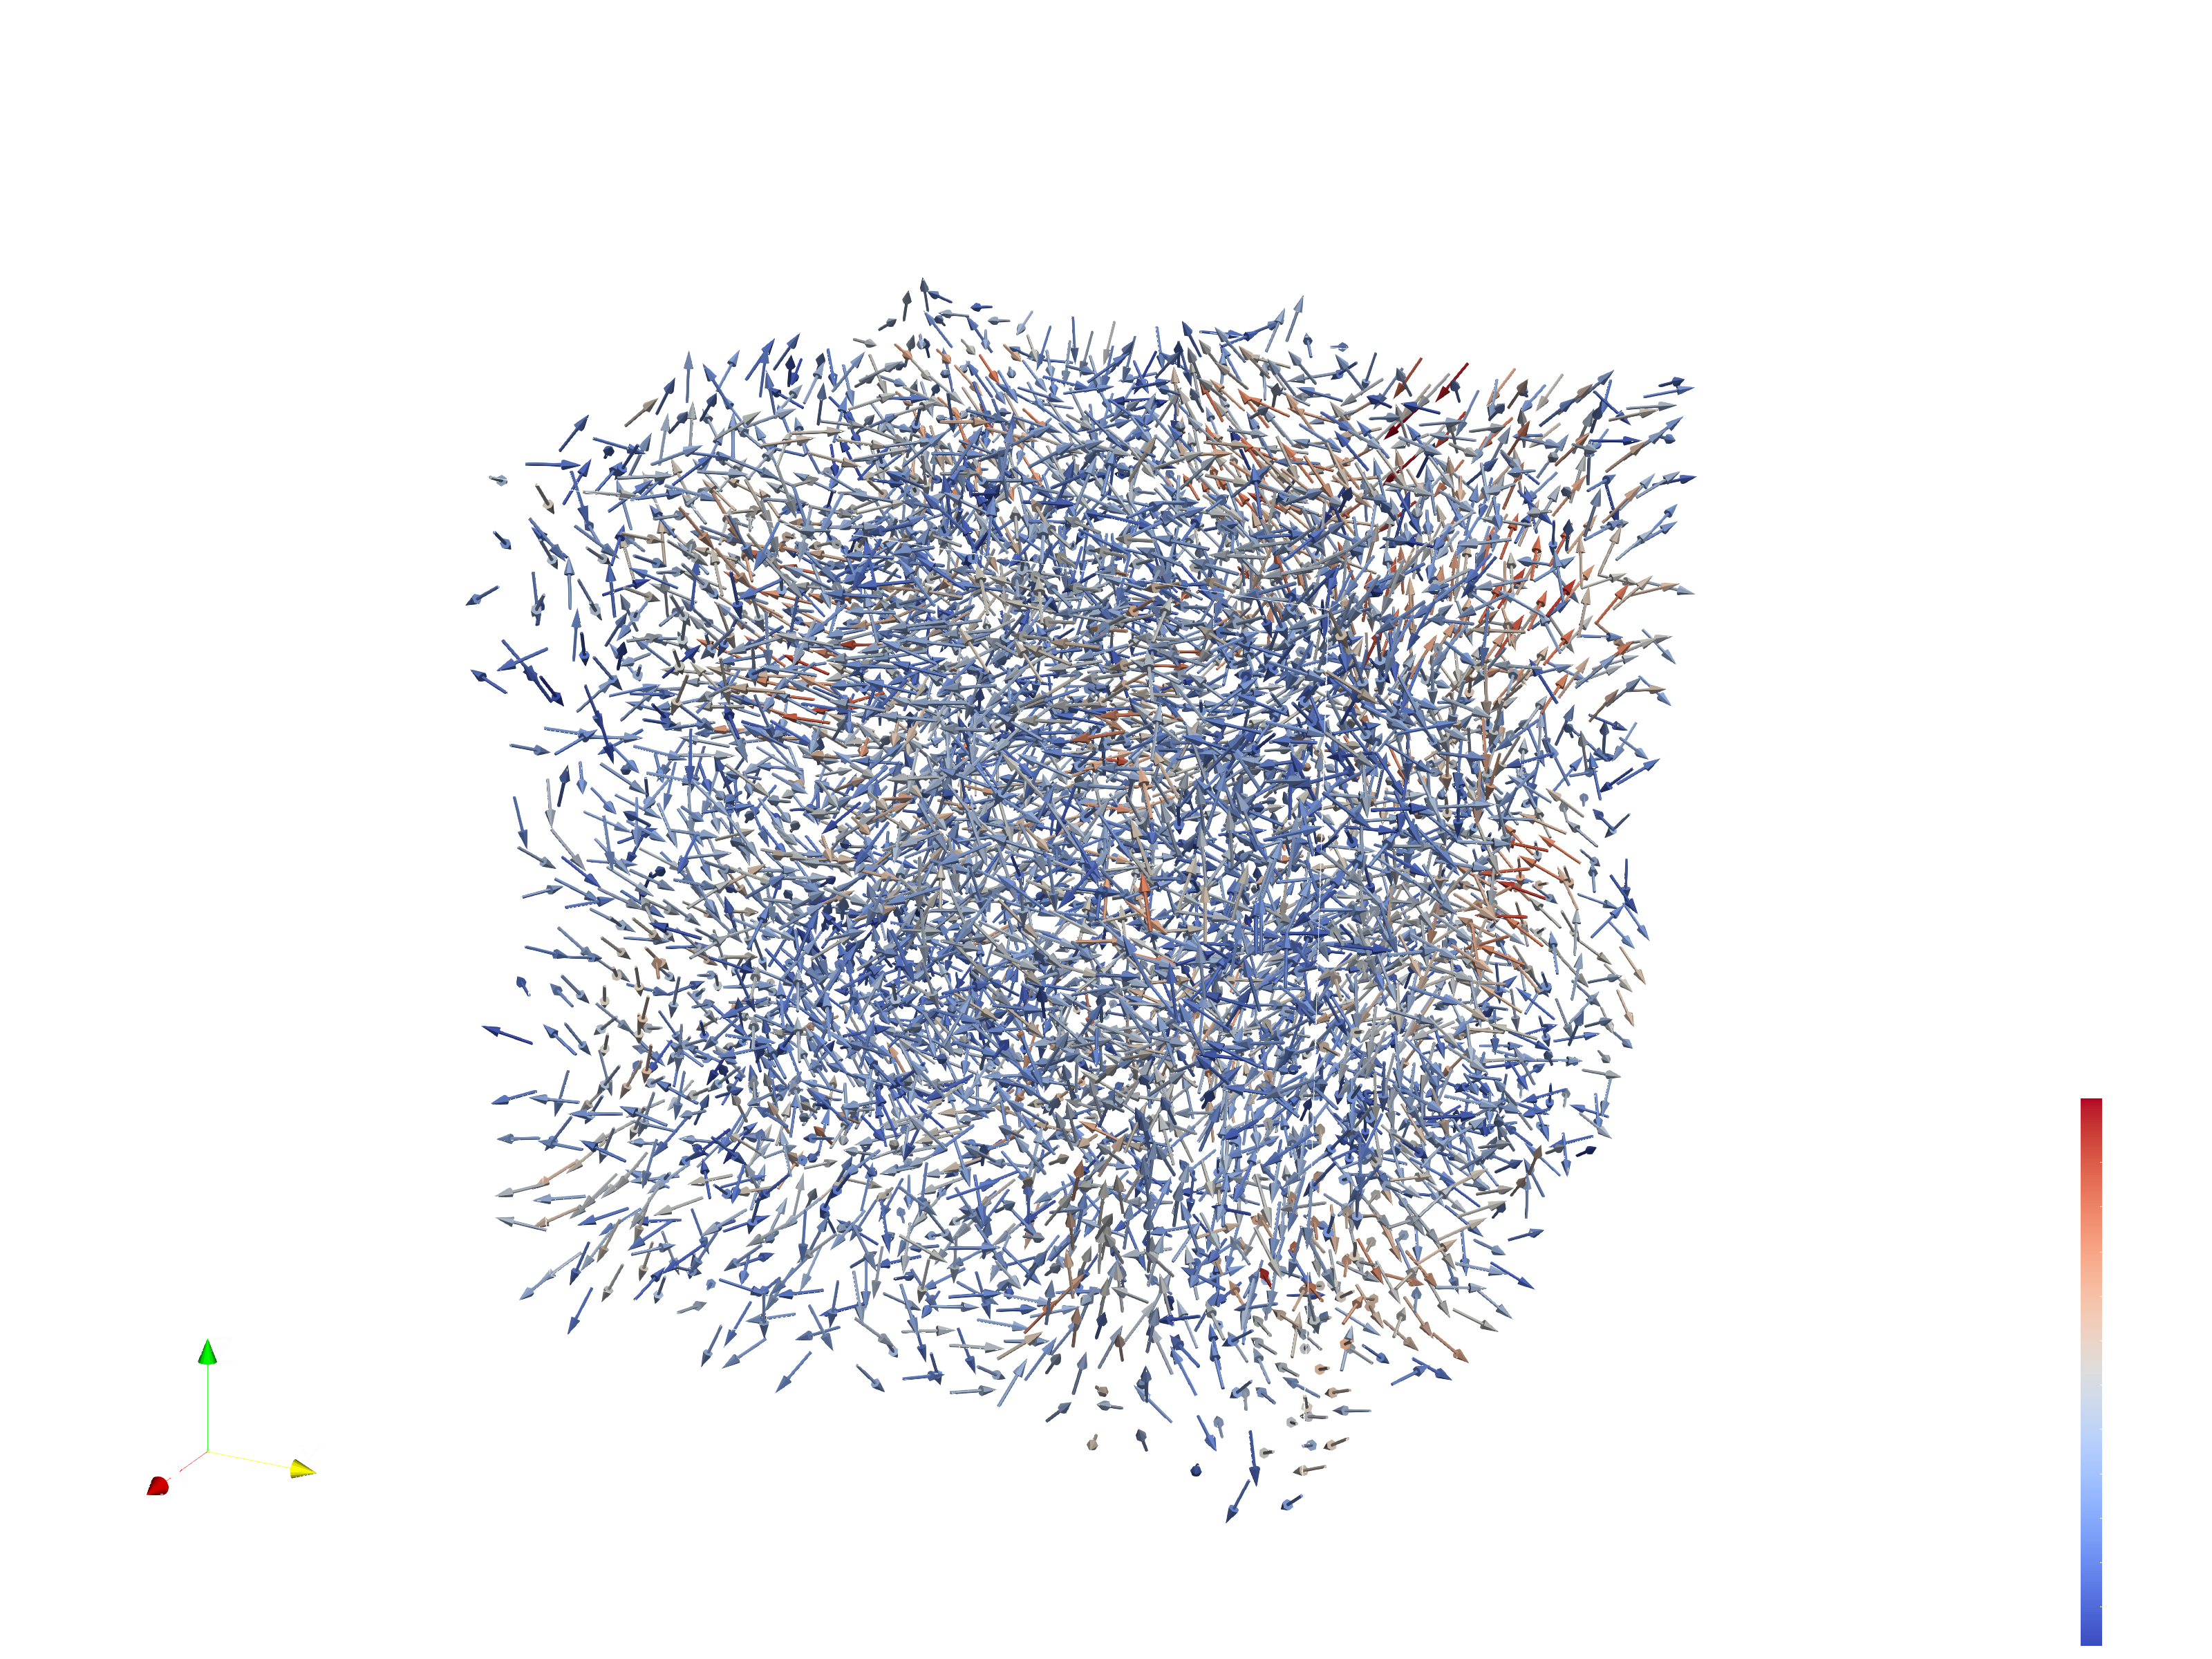
\includegraphics[width=0.4\linewidth]{images/kriging/3components/full_field_velocity_field.png}}%
        \hfill       
        \subcaptionbox{плоскость $xy$, $z = 0$\label{img:slice_velcotiy_field_xy_znormal_angle_1}} 
        {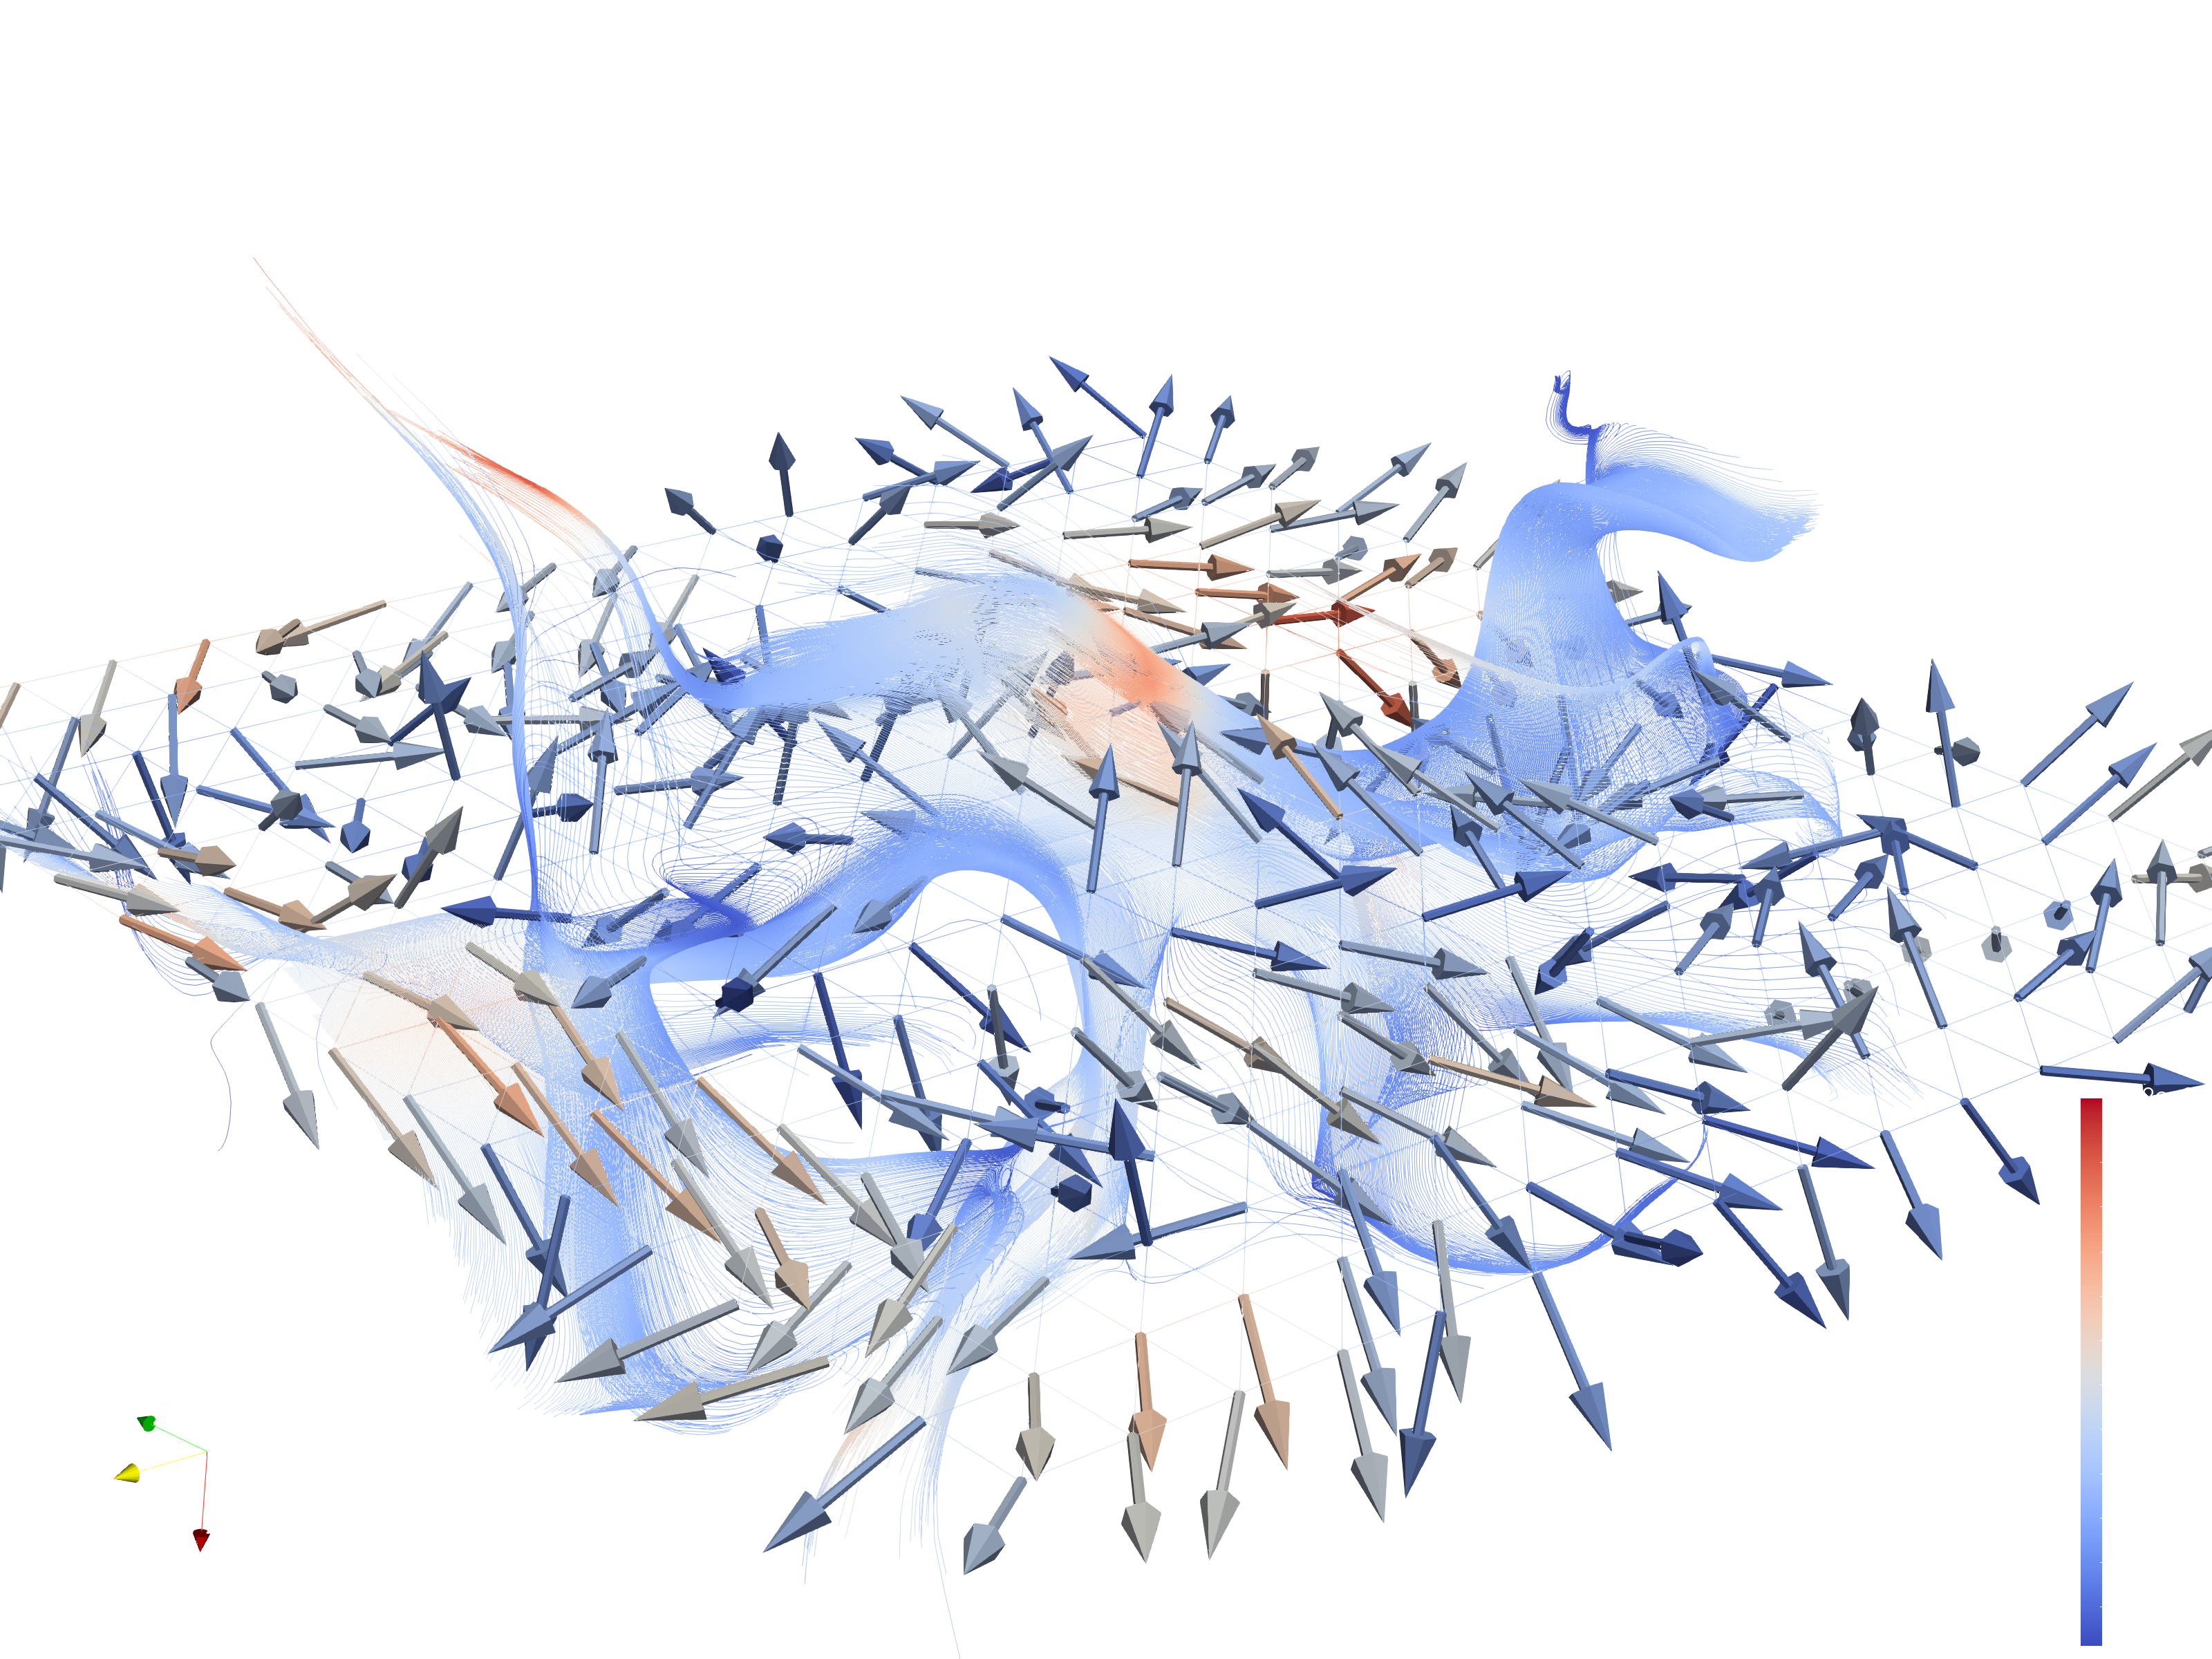
\includegraphics[width=0.4\linewidth]{images/kriging/3components/z_normal_xyplane_on_angle_with_stream_trace.png}} \\
        \hfill
        \subcaptionbox[List-of-Figures entry]{плоскость $xy$, $z = 0$\label{img:slice_velcotiy_field_xy_znormal_angle_2}} 
        {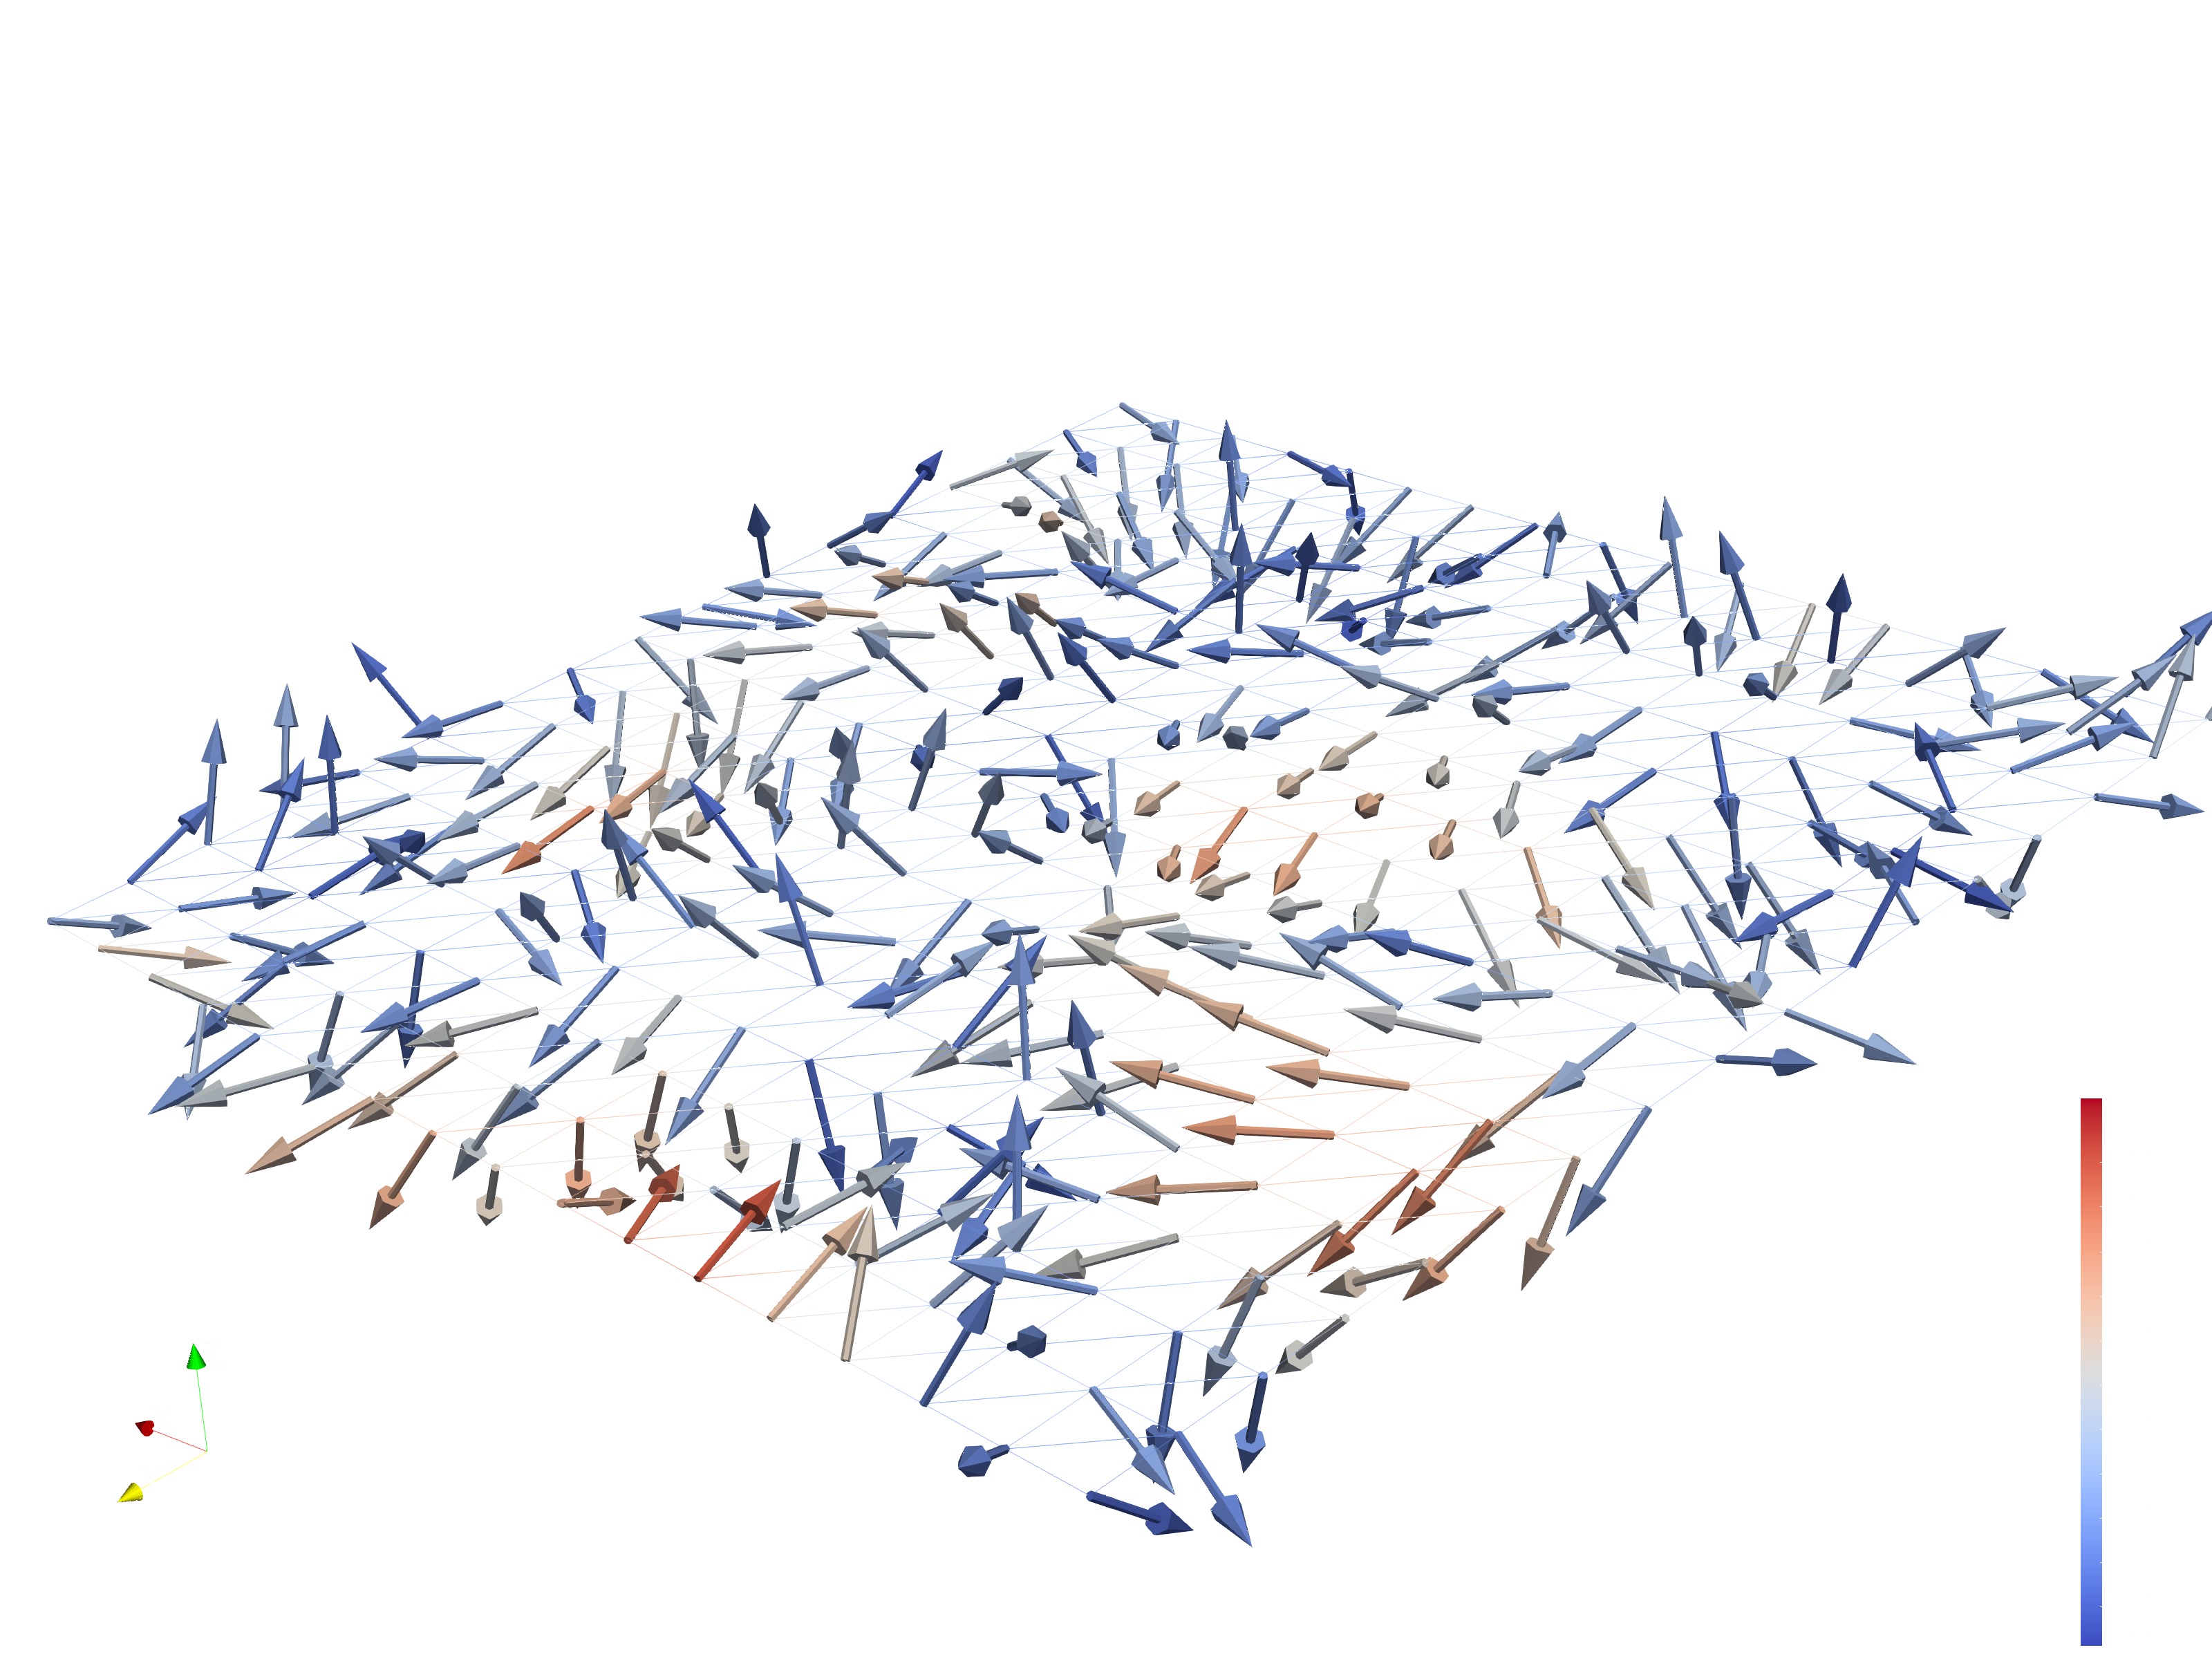
\includegraphics[width=0.4\linewidth]{images/kriging/3components/z_normal_xyplane_on_angle.png}}%
        \hfill       
        \subcaptionbox{плоскость $xy$, $z = 0$\label{img:slice_velcotiy_field_xy_znormal_no_angle}} 
        {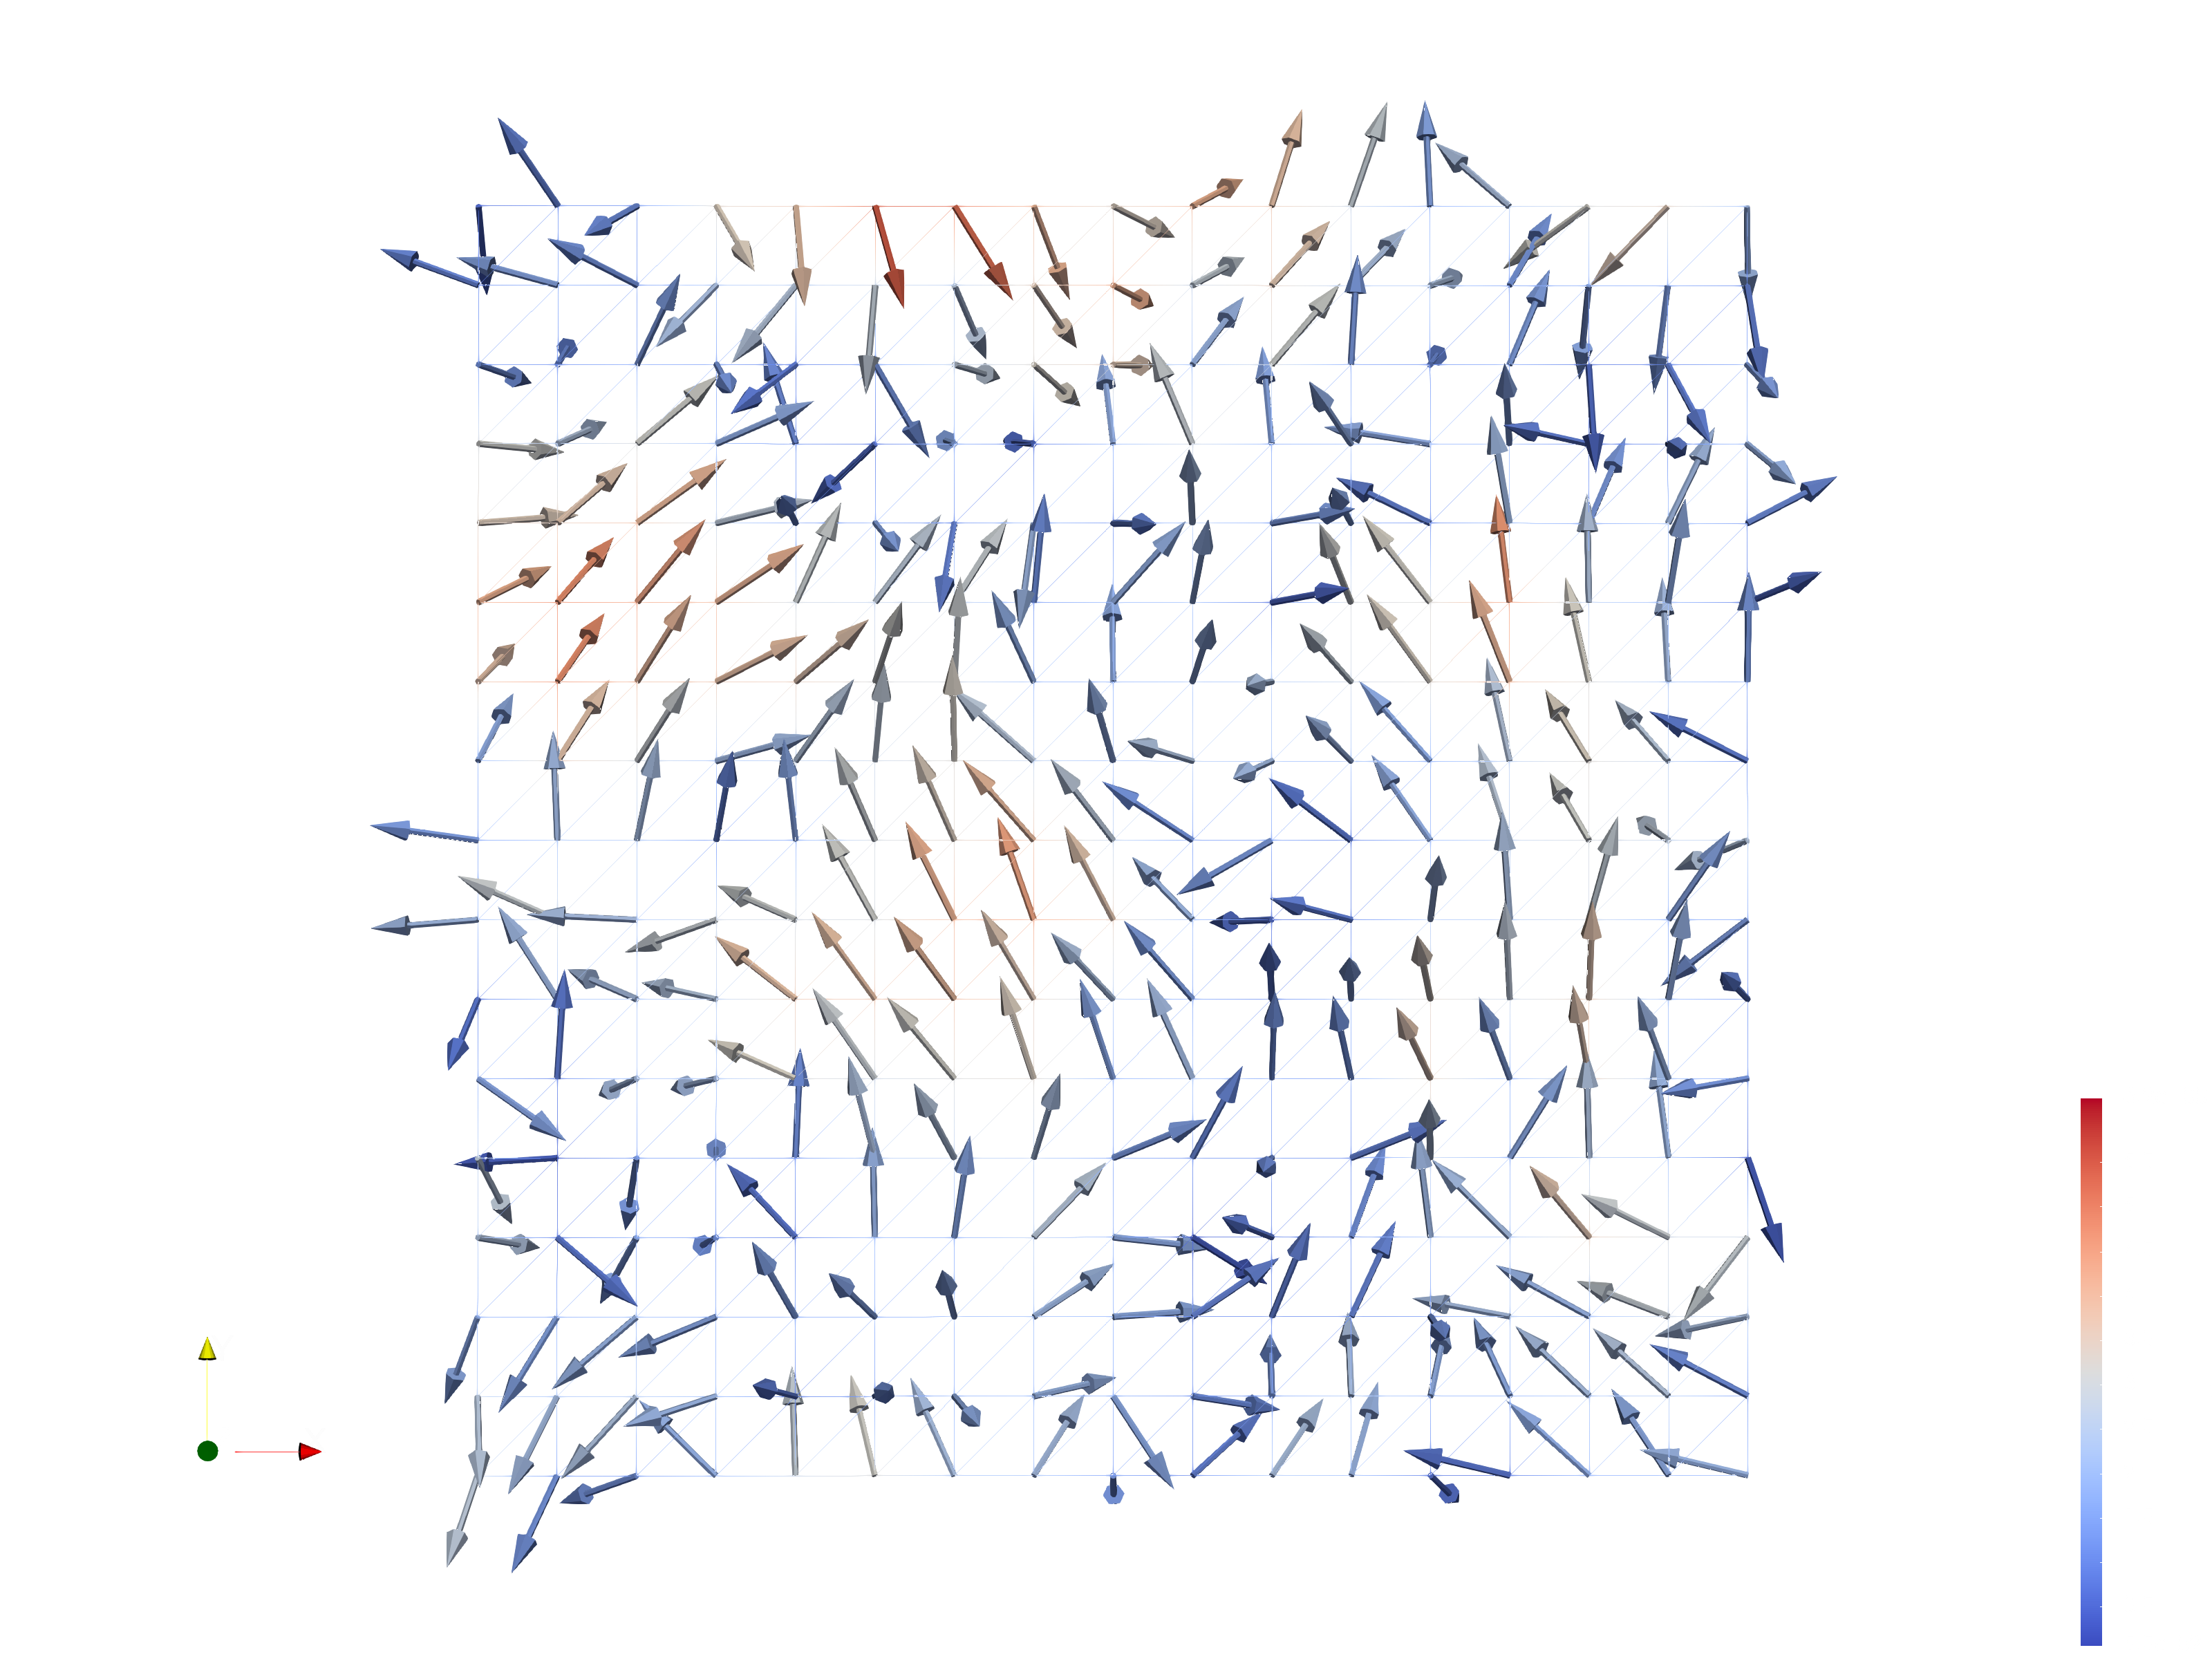
\includegraphics[width=0.4\linewidth]{images/kriging/3components/z_normal_xyplane.png}}
        \hfill
    }
    
    \onehalfspacing{Поле на картинке б представлено с линиями тока, расчитанными вдоль оси $y$}
    \caption{Поле флуктуаций сгенерированных трёхмерным стохастическим методом, цветом обозначена амплитуда флуктуаций}
    \label{img:velocity_fluctuation_field_forkriging}  
\end{figure}

Приведём тепловые карты тензора ковариаций полученного из целевого спектра при помощи \eqref{eq:part3_2} и \eqref{eq:kriging_equation14_2}.

%
% Точная ковариация
%
\begin{figure}[!h]
    \center{
        \hfill
        \subcaptionbox[List-of-Figures entry]{$R_{xx}$  $x$-нормаль\label{img:kriging_exact_cov_r_11}} 
        {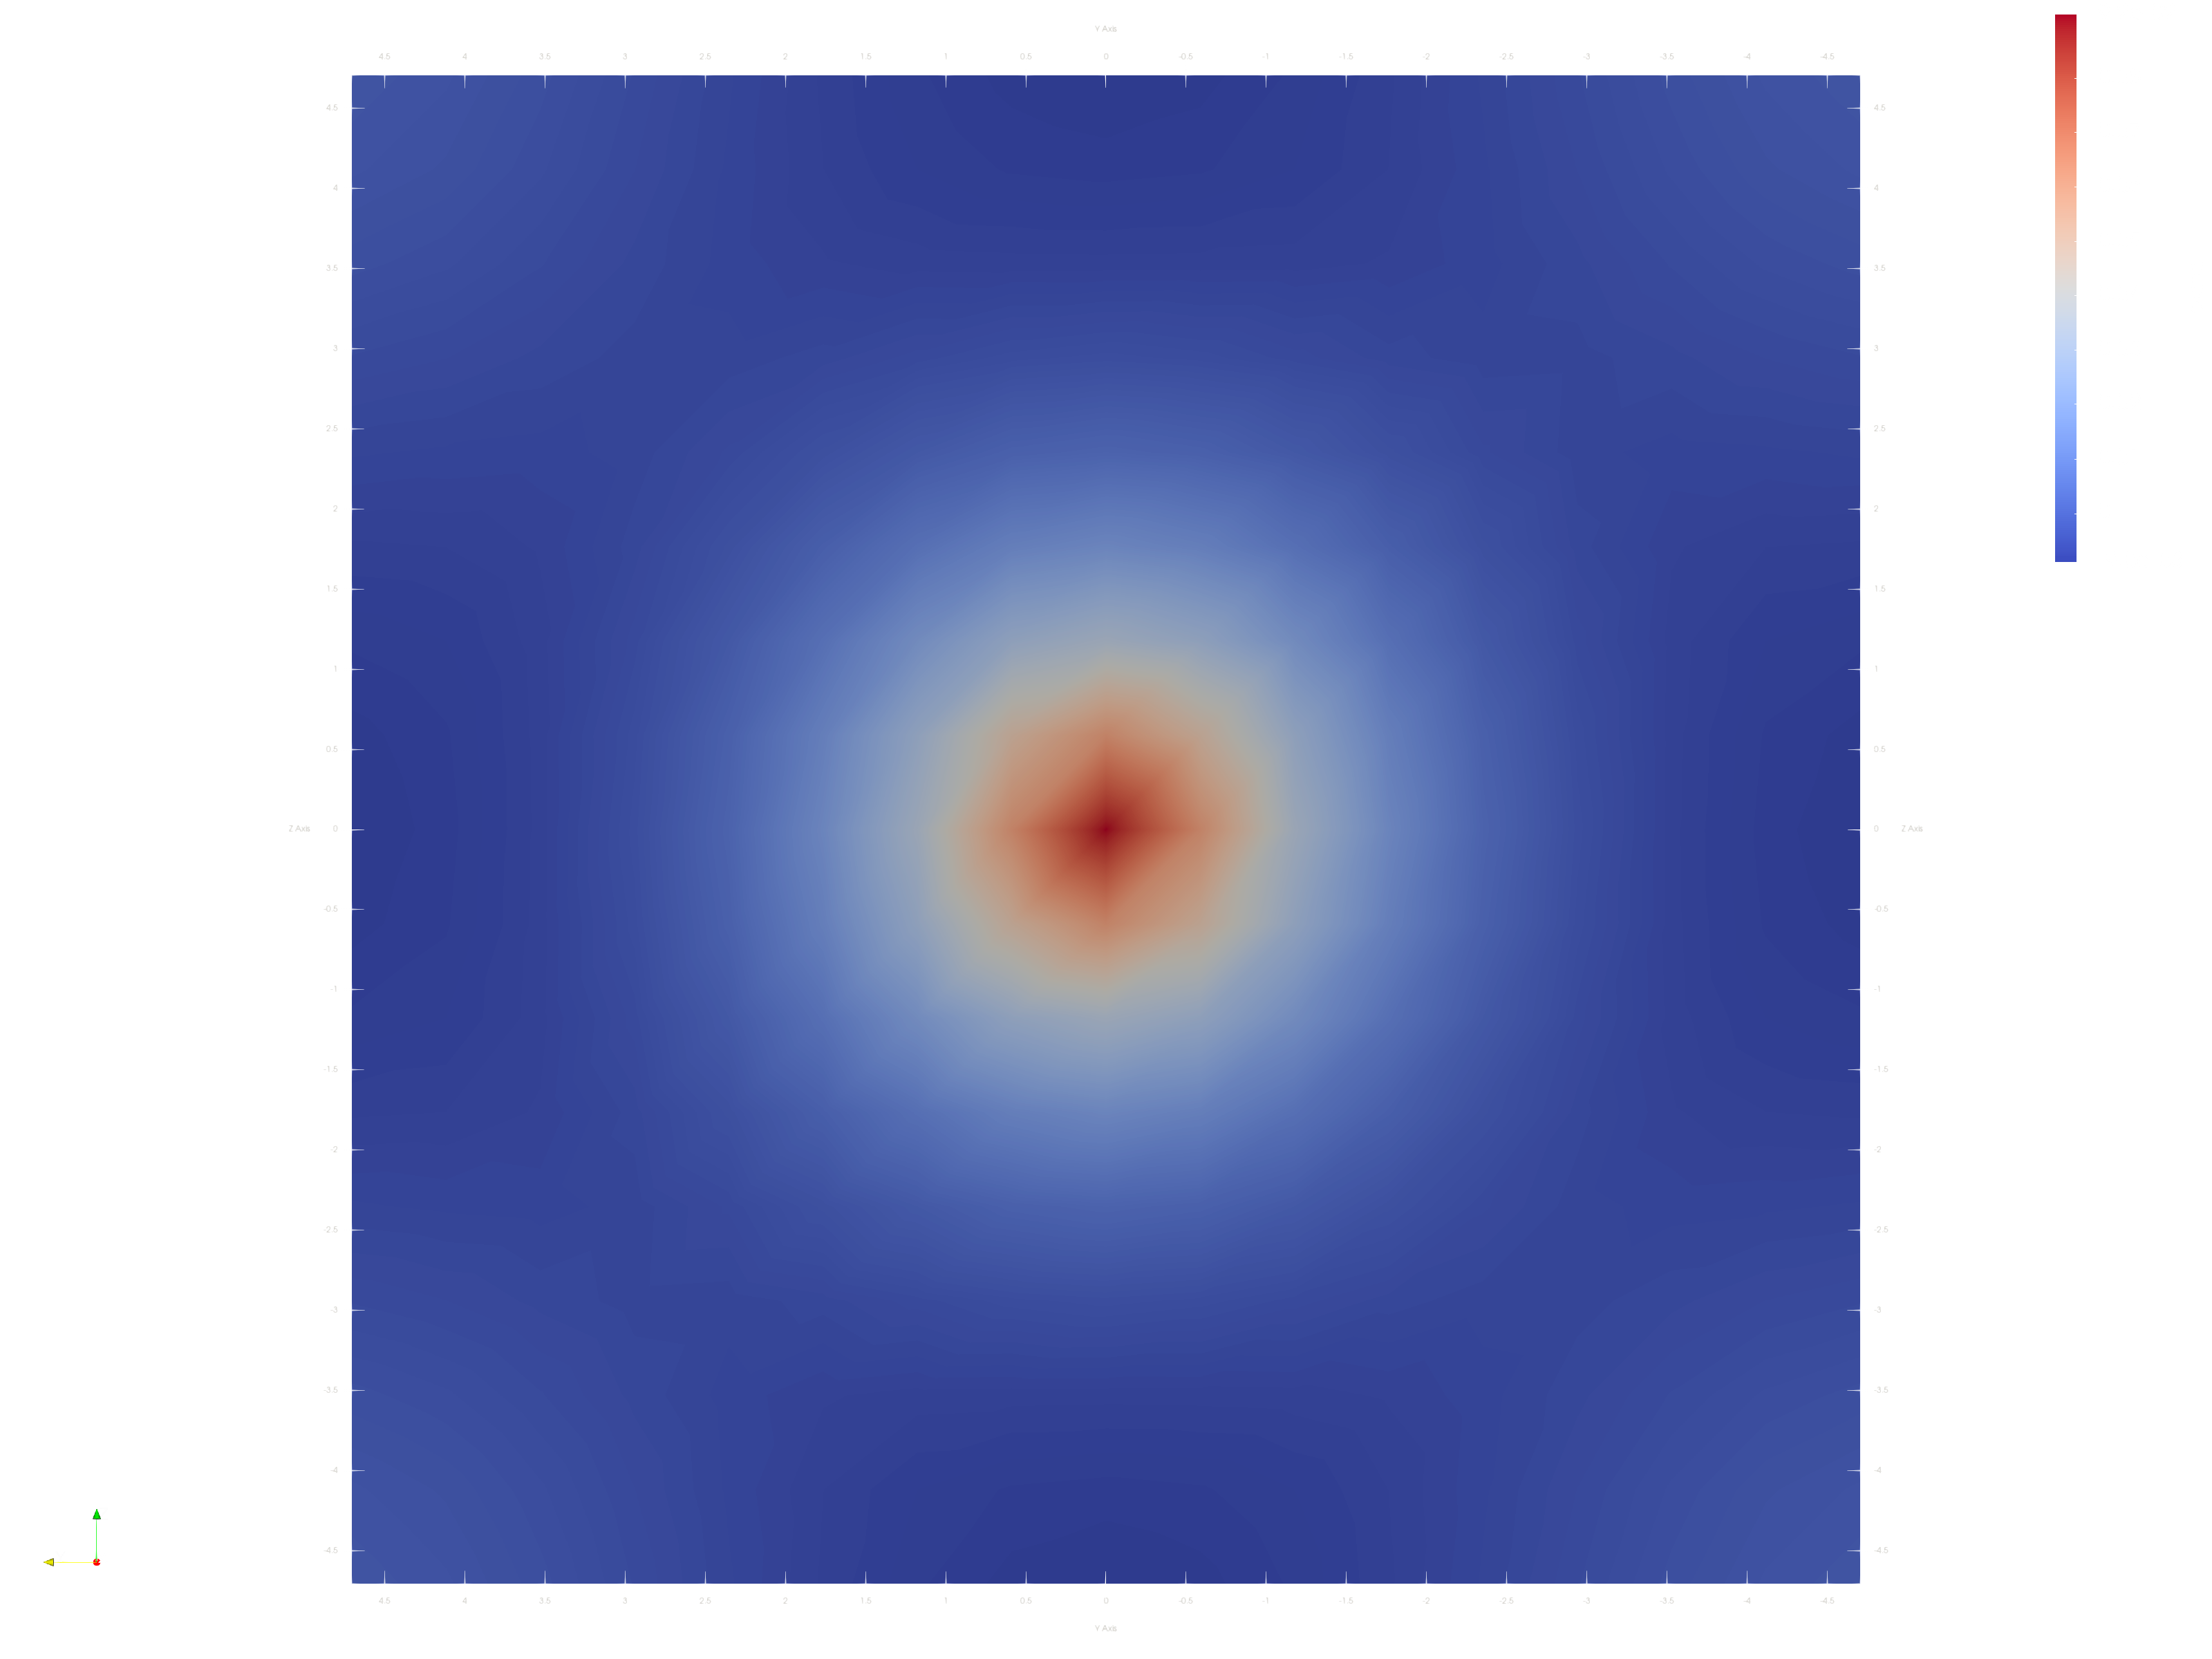
\includegraphics[width=0.32\linewidth]{images/kriging/3components/exact_cov_11_xx.png}}%
        \hfill       
        \subcaptionbox{$R_{xx}$  $y$-нормаль \label{img:kriging_exact_cov_r_12}} 
        {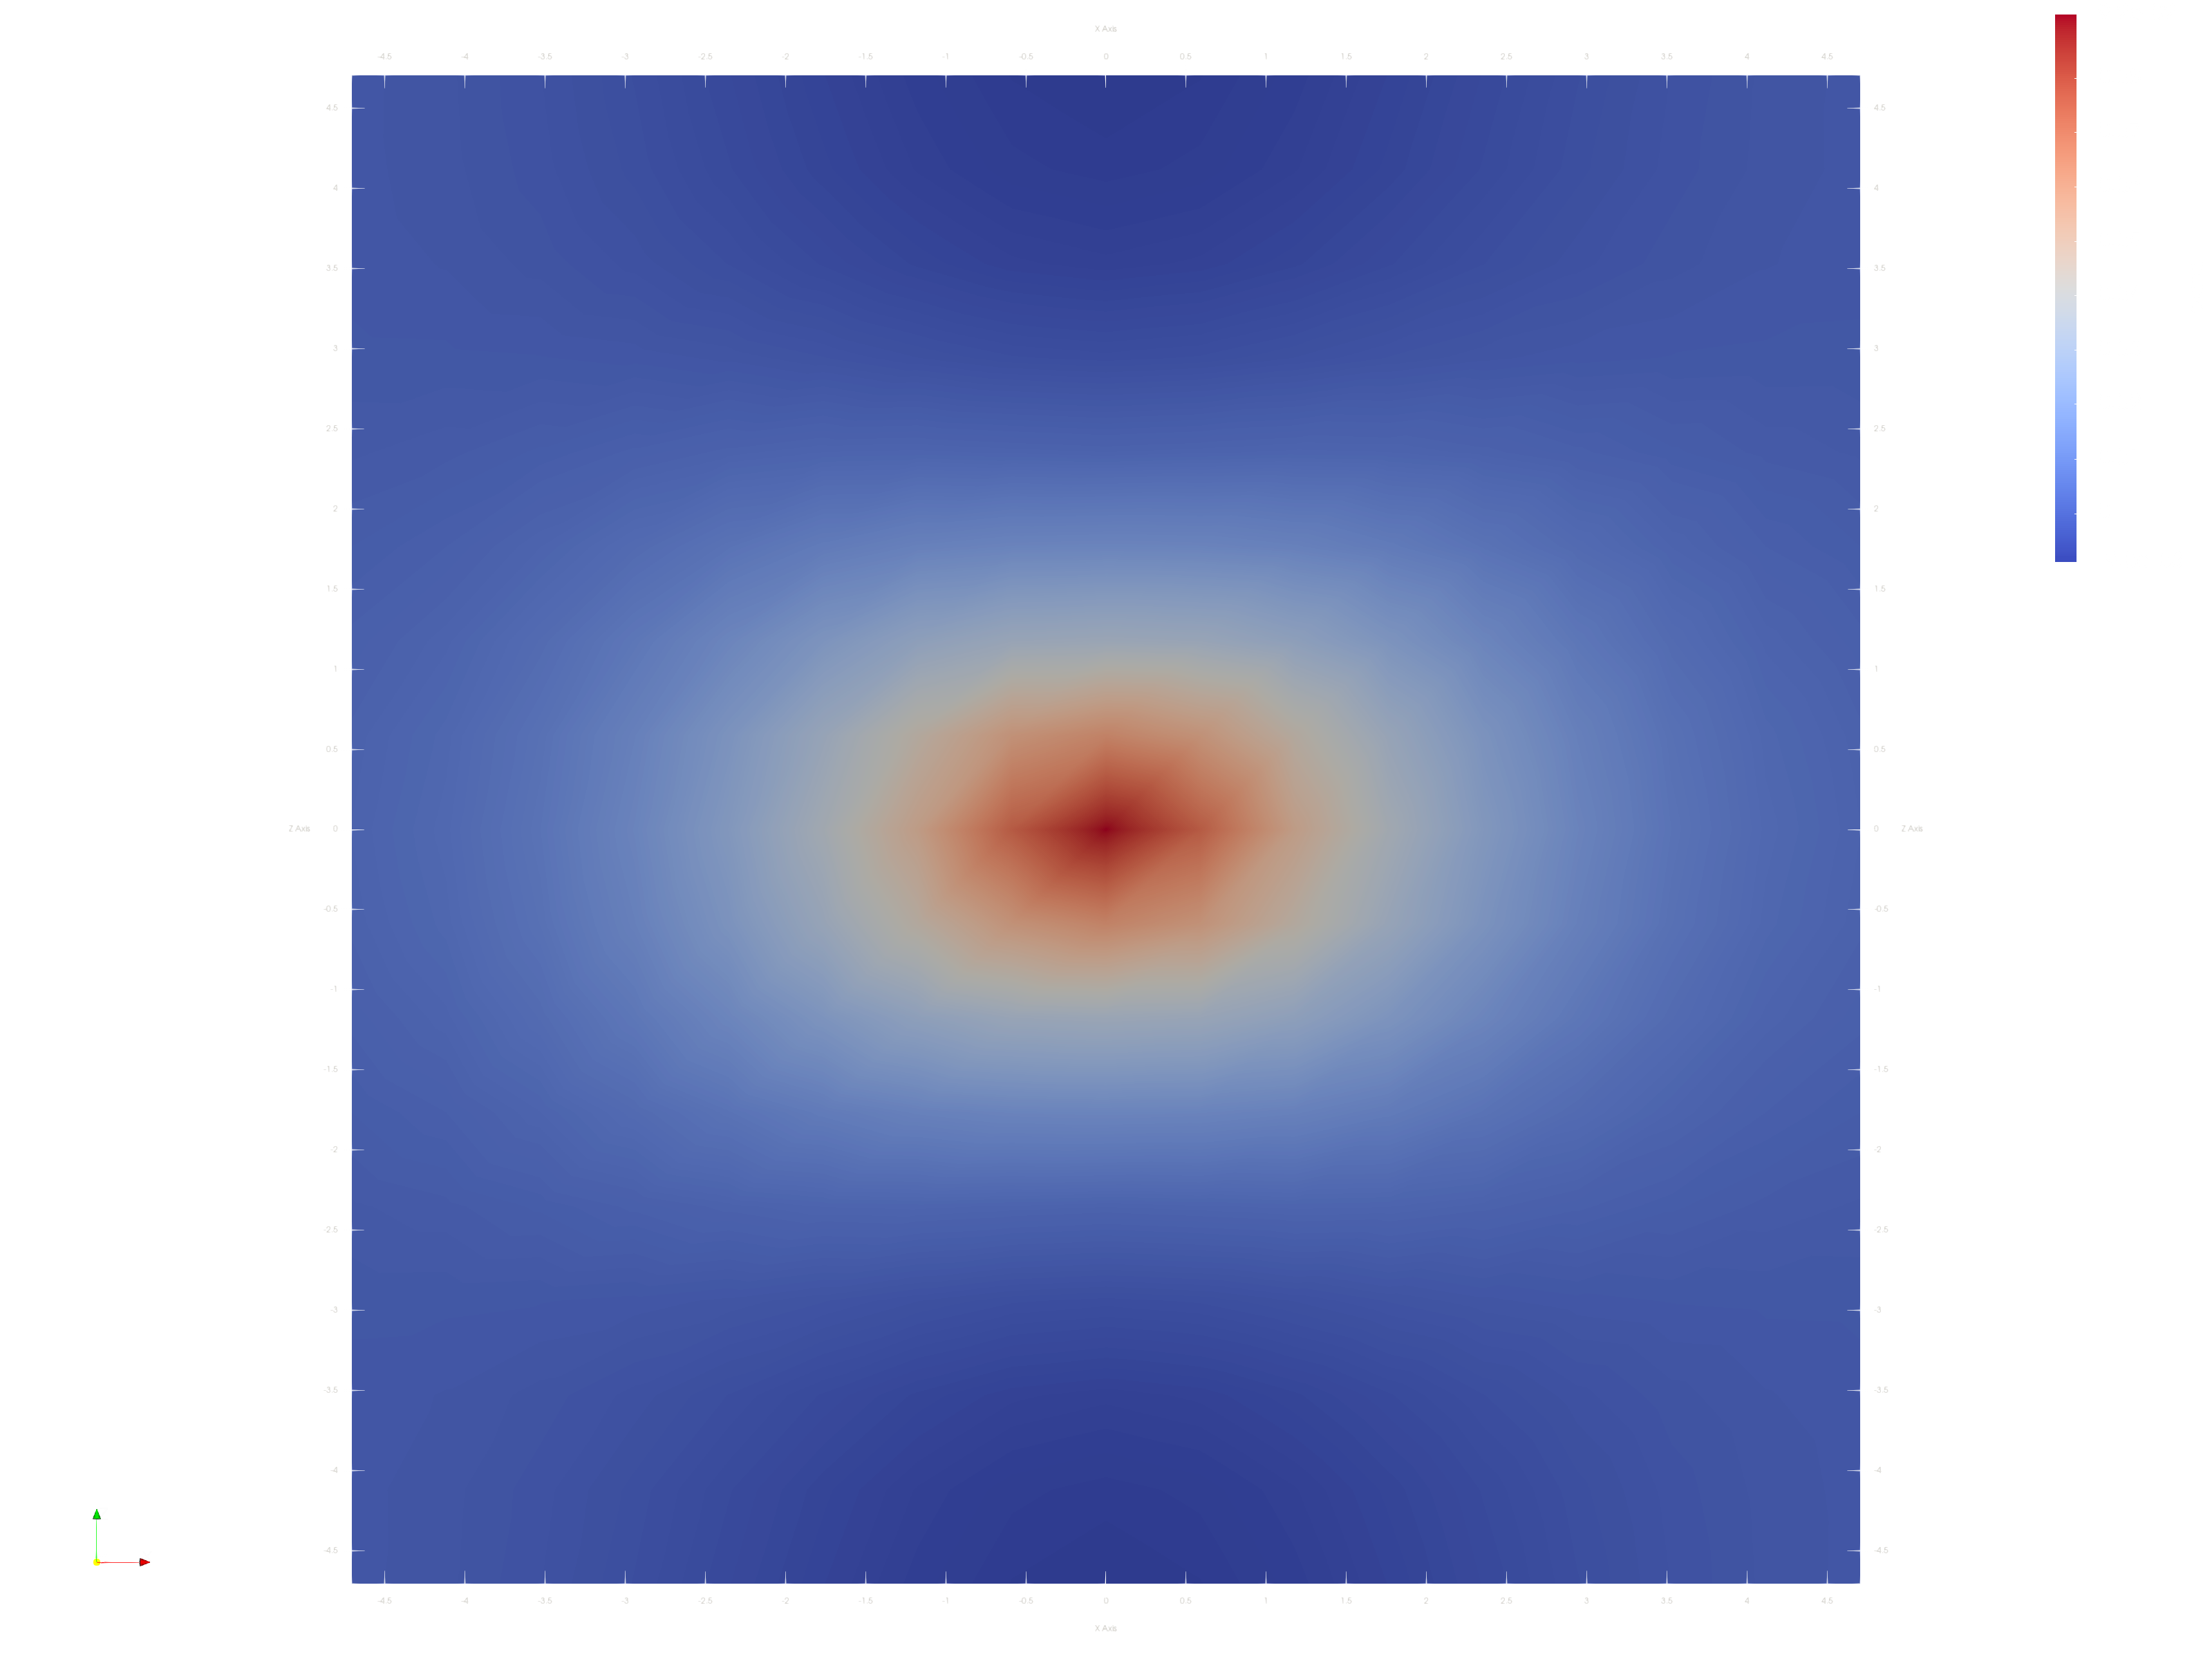
\includegraphics[width=0.32\linewidth]{images/kriging/3components/exact_cov_11_yy.png}}
        \hfill
        \subcaptionbox{$R_{xx}$  $z$-нормаль\label{img:kriging_exact_cov_r_13}} 
        {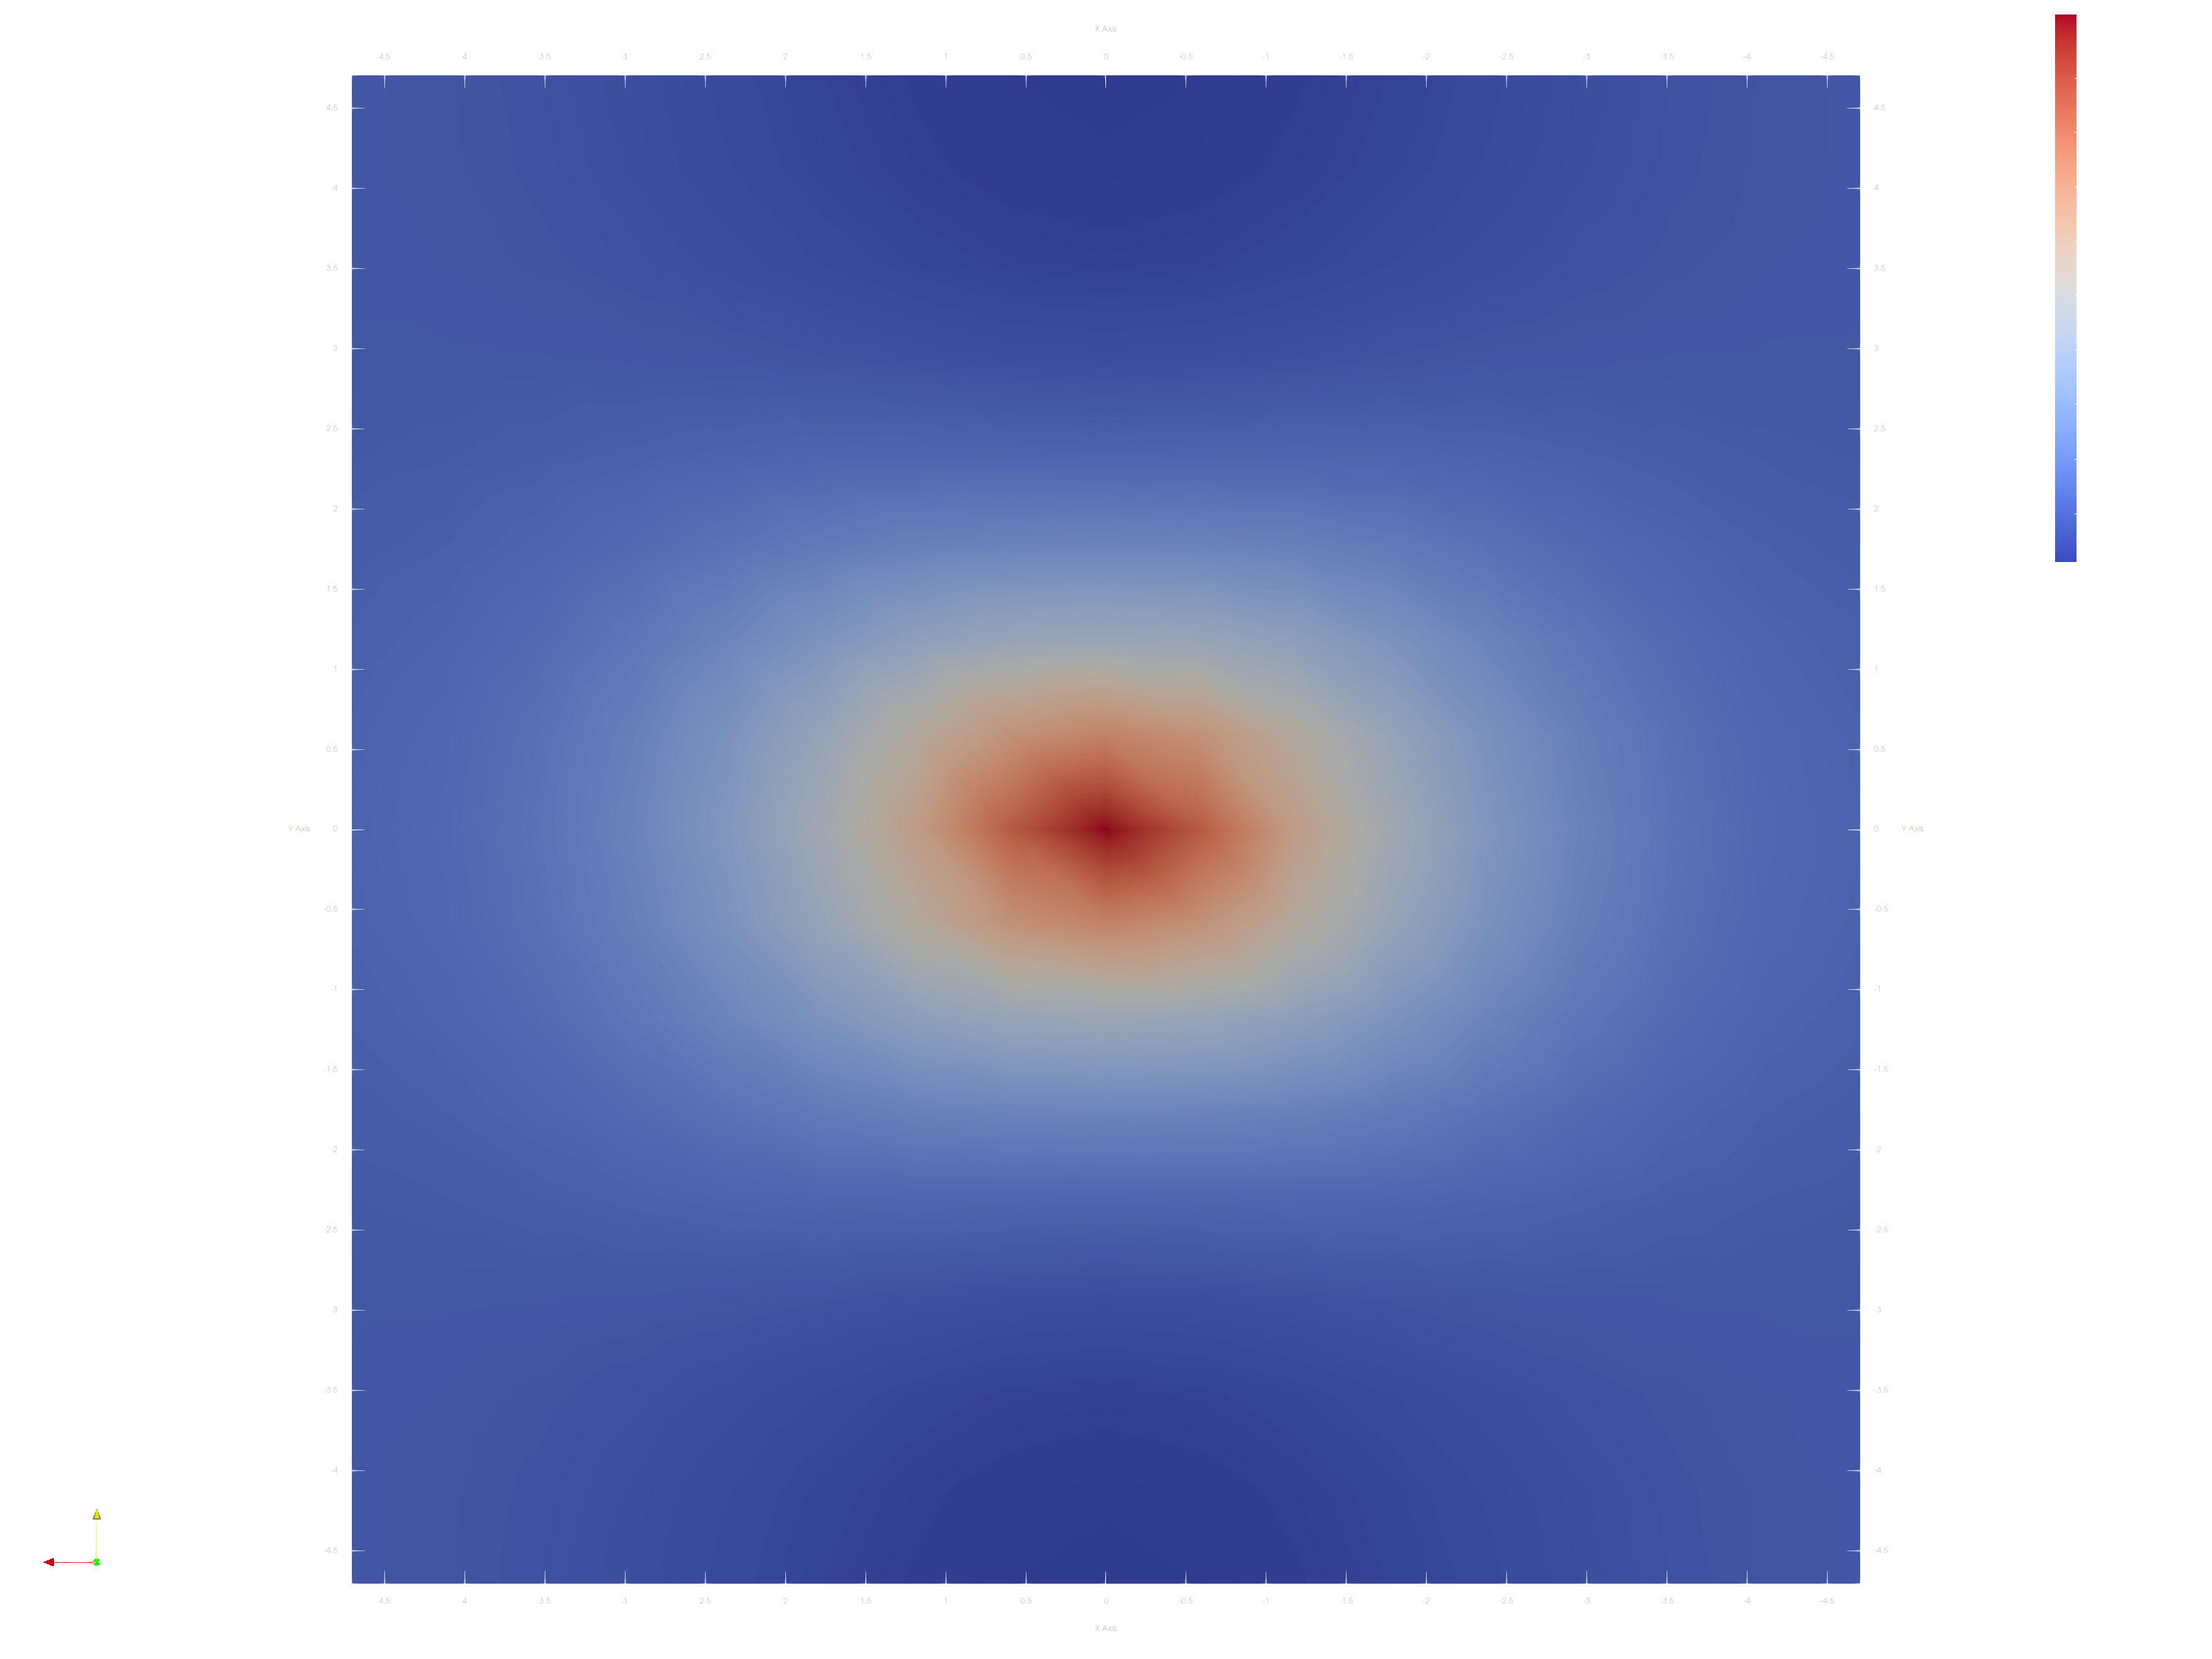
\includegraphics[width=0.32\linewidth]{images/kriging/3components/exact_cov_11_zz.png}}%
        \hfill       
        
        \subcaptionbox{$R_{yy}$ $x$-нормаль \label{img:kriging_exact_cov_r_22}} 
        {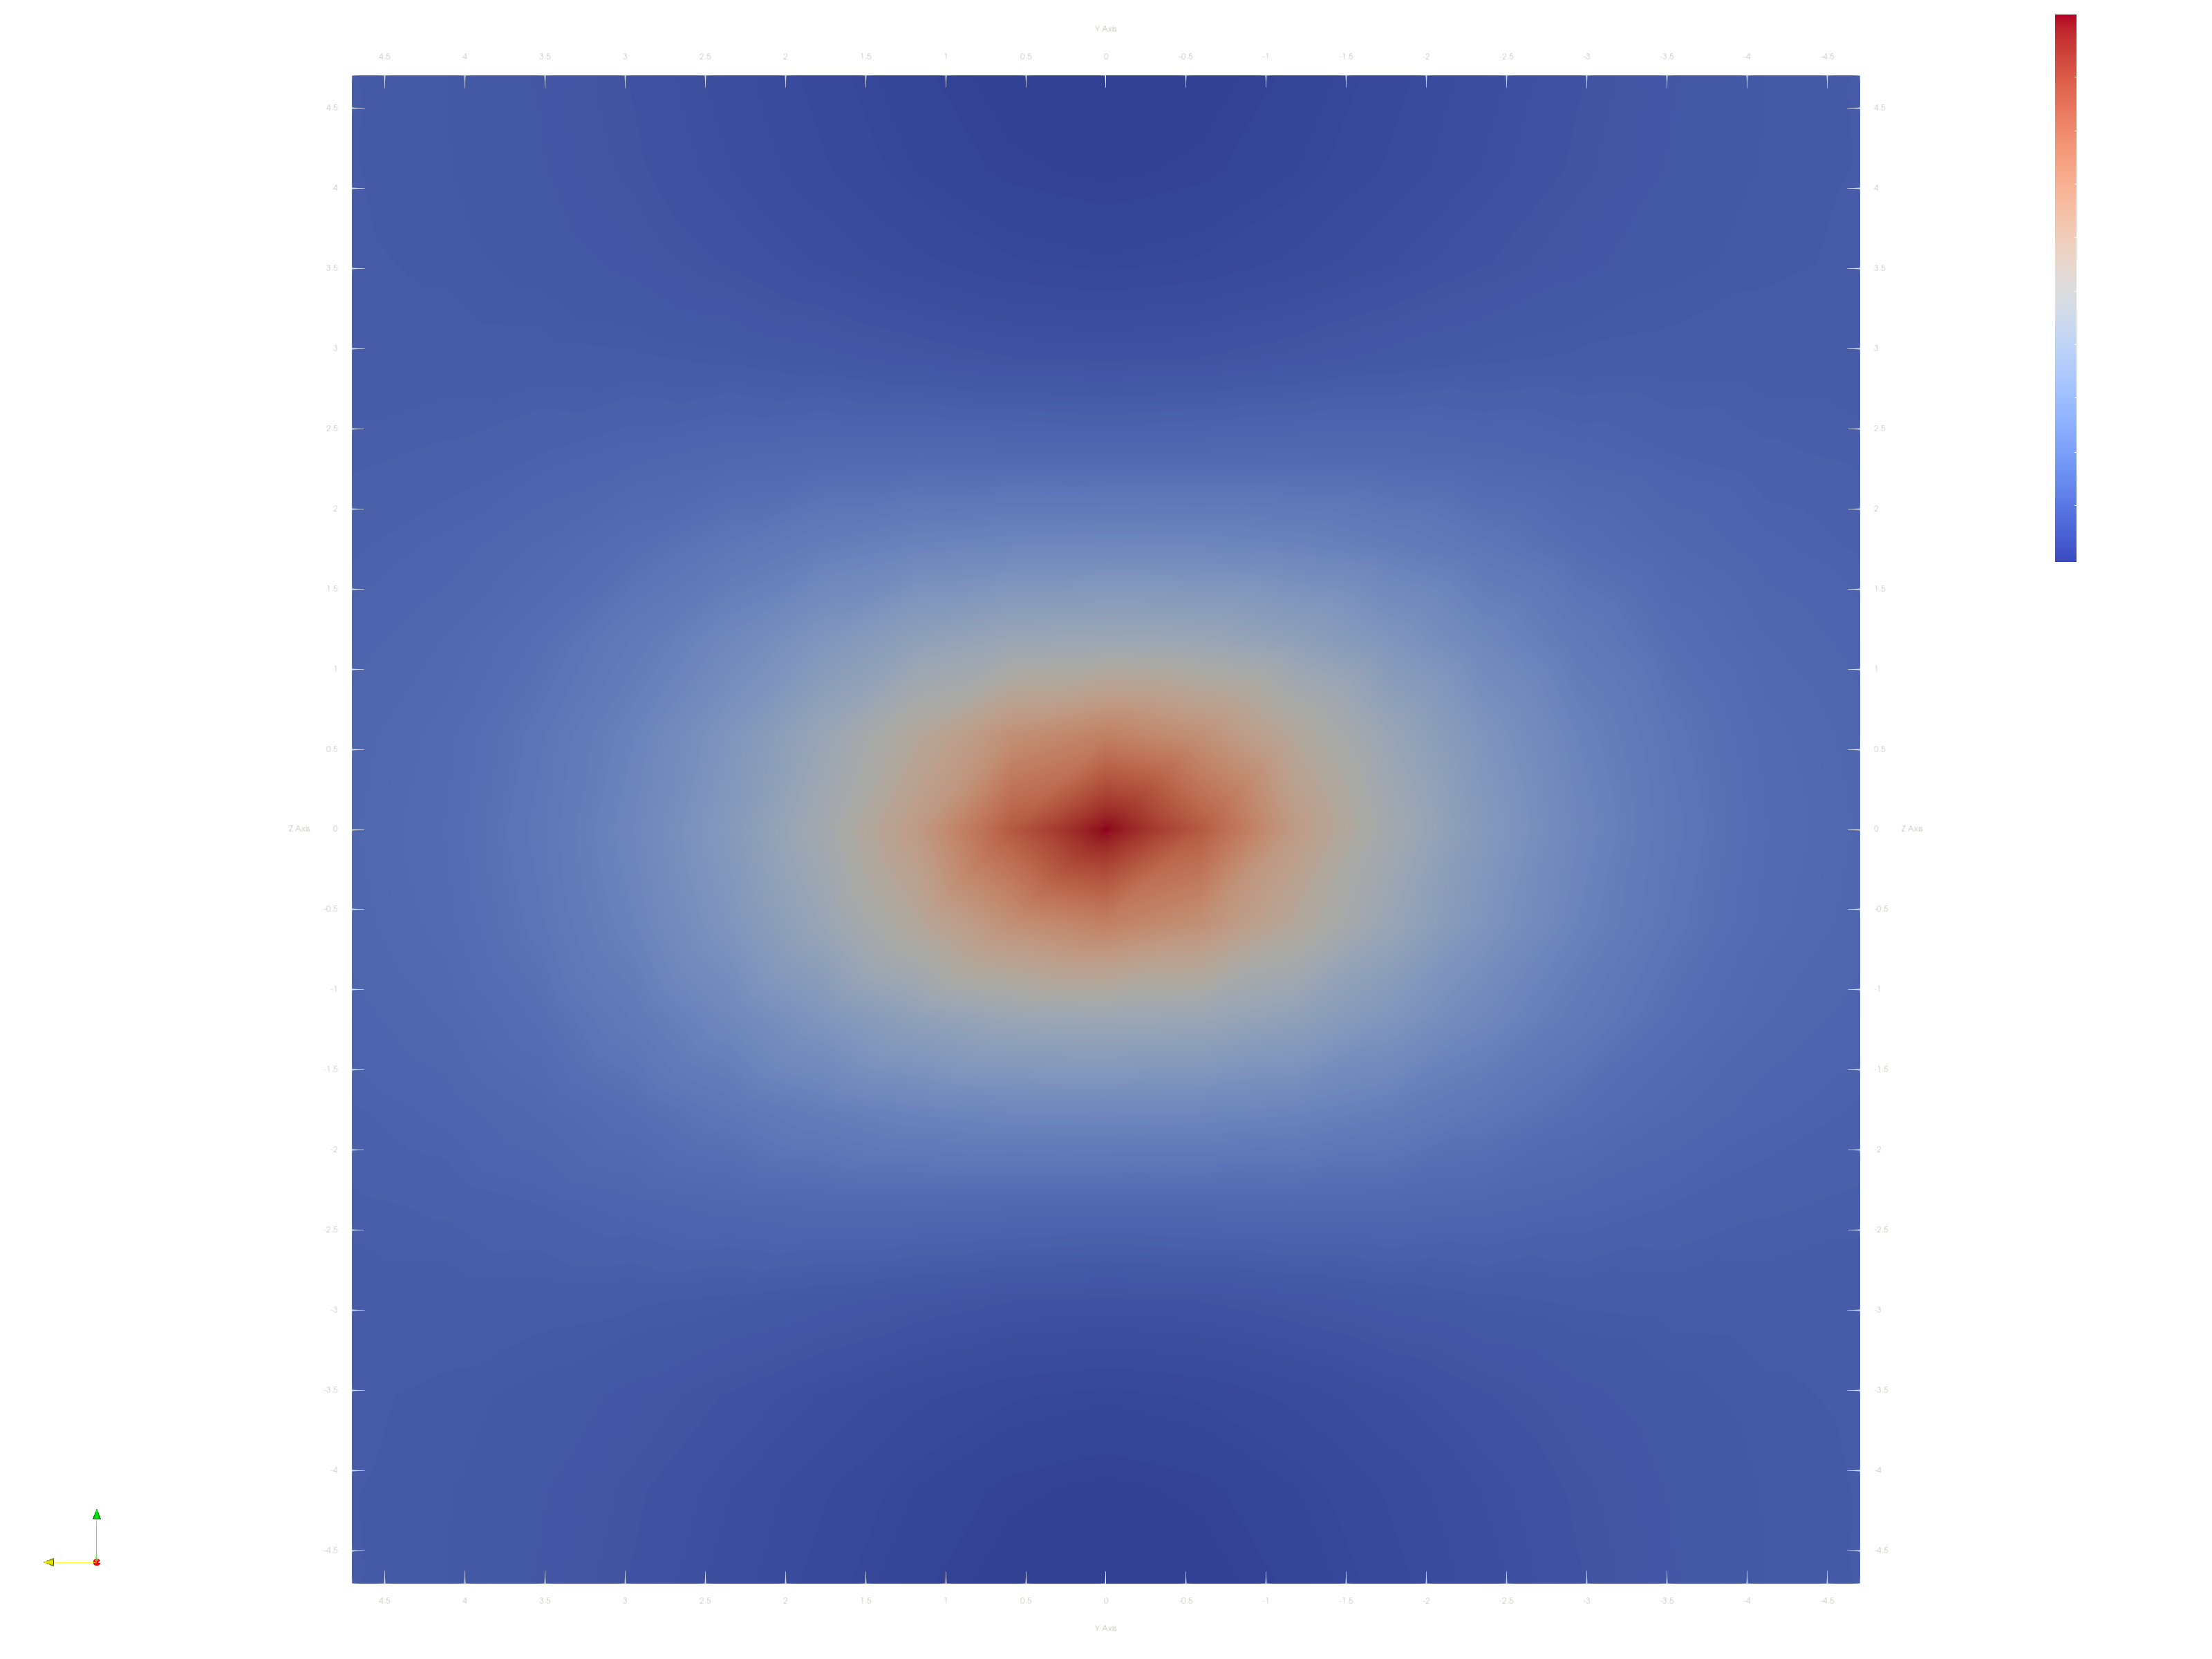
\includegraphics[width=0.32\linewidth]{images/kriging/3components/exact_cov_22_xx.png}}
        \hfill
        \subcaptionbox{$R_{yy}$ $y$-нормаль \label{img:kriging_exact_cov_r_23}} 
        {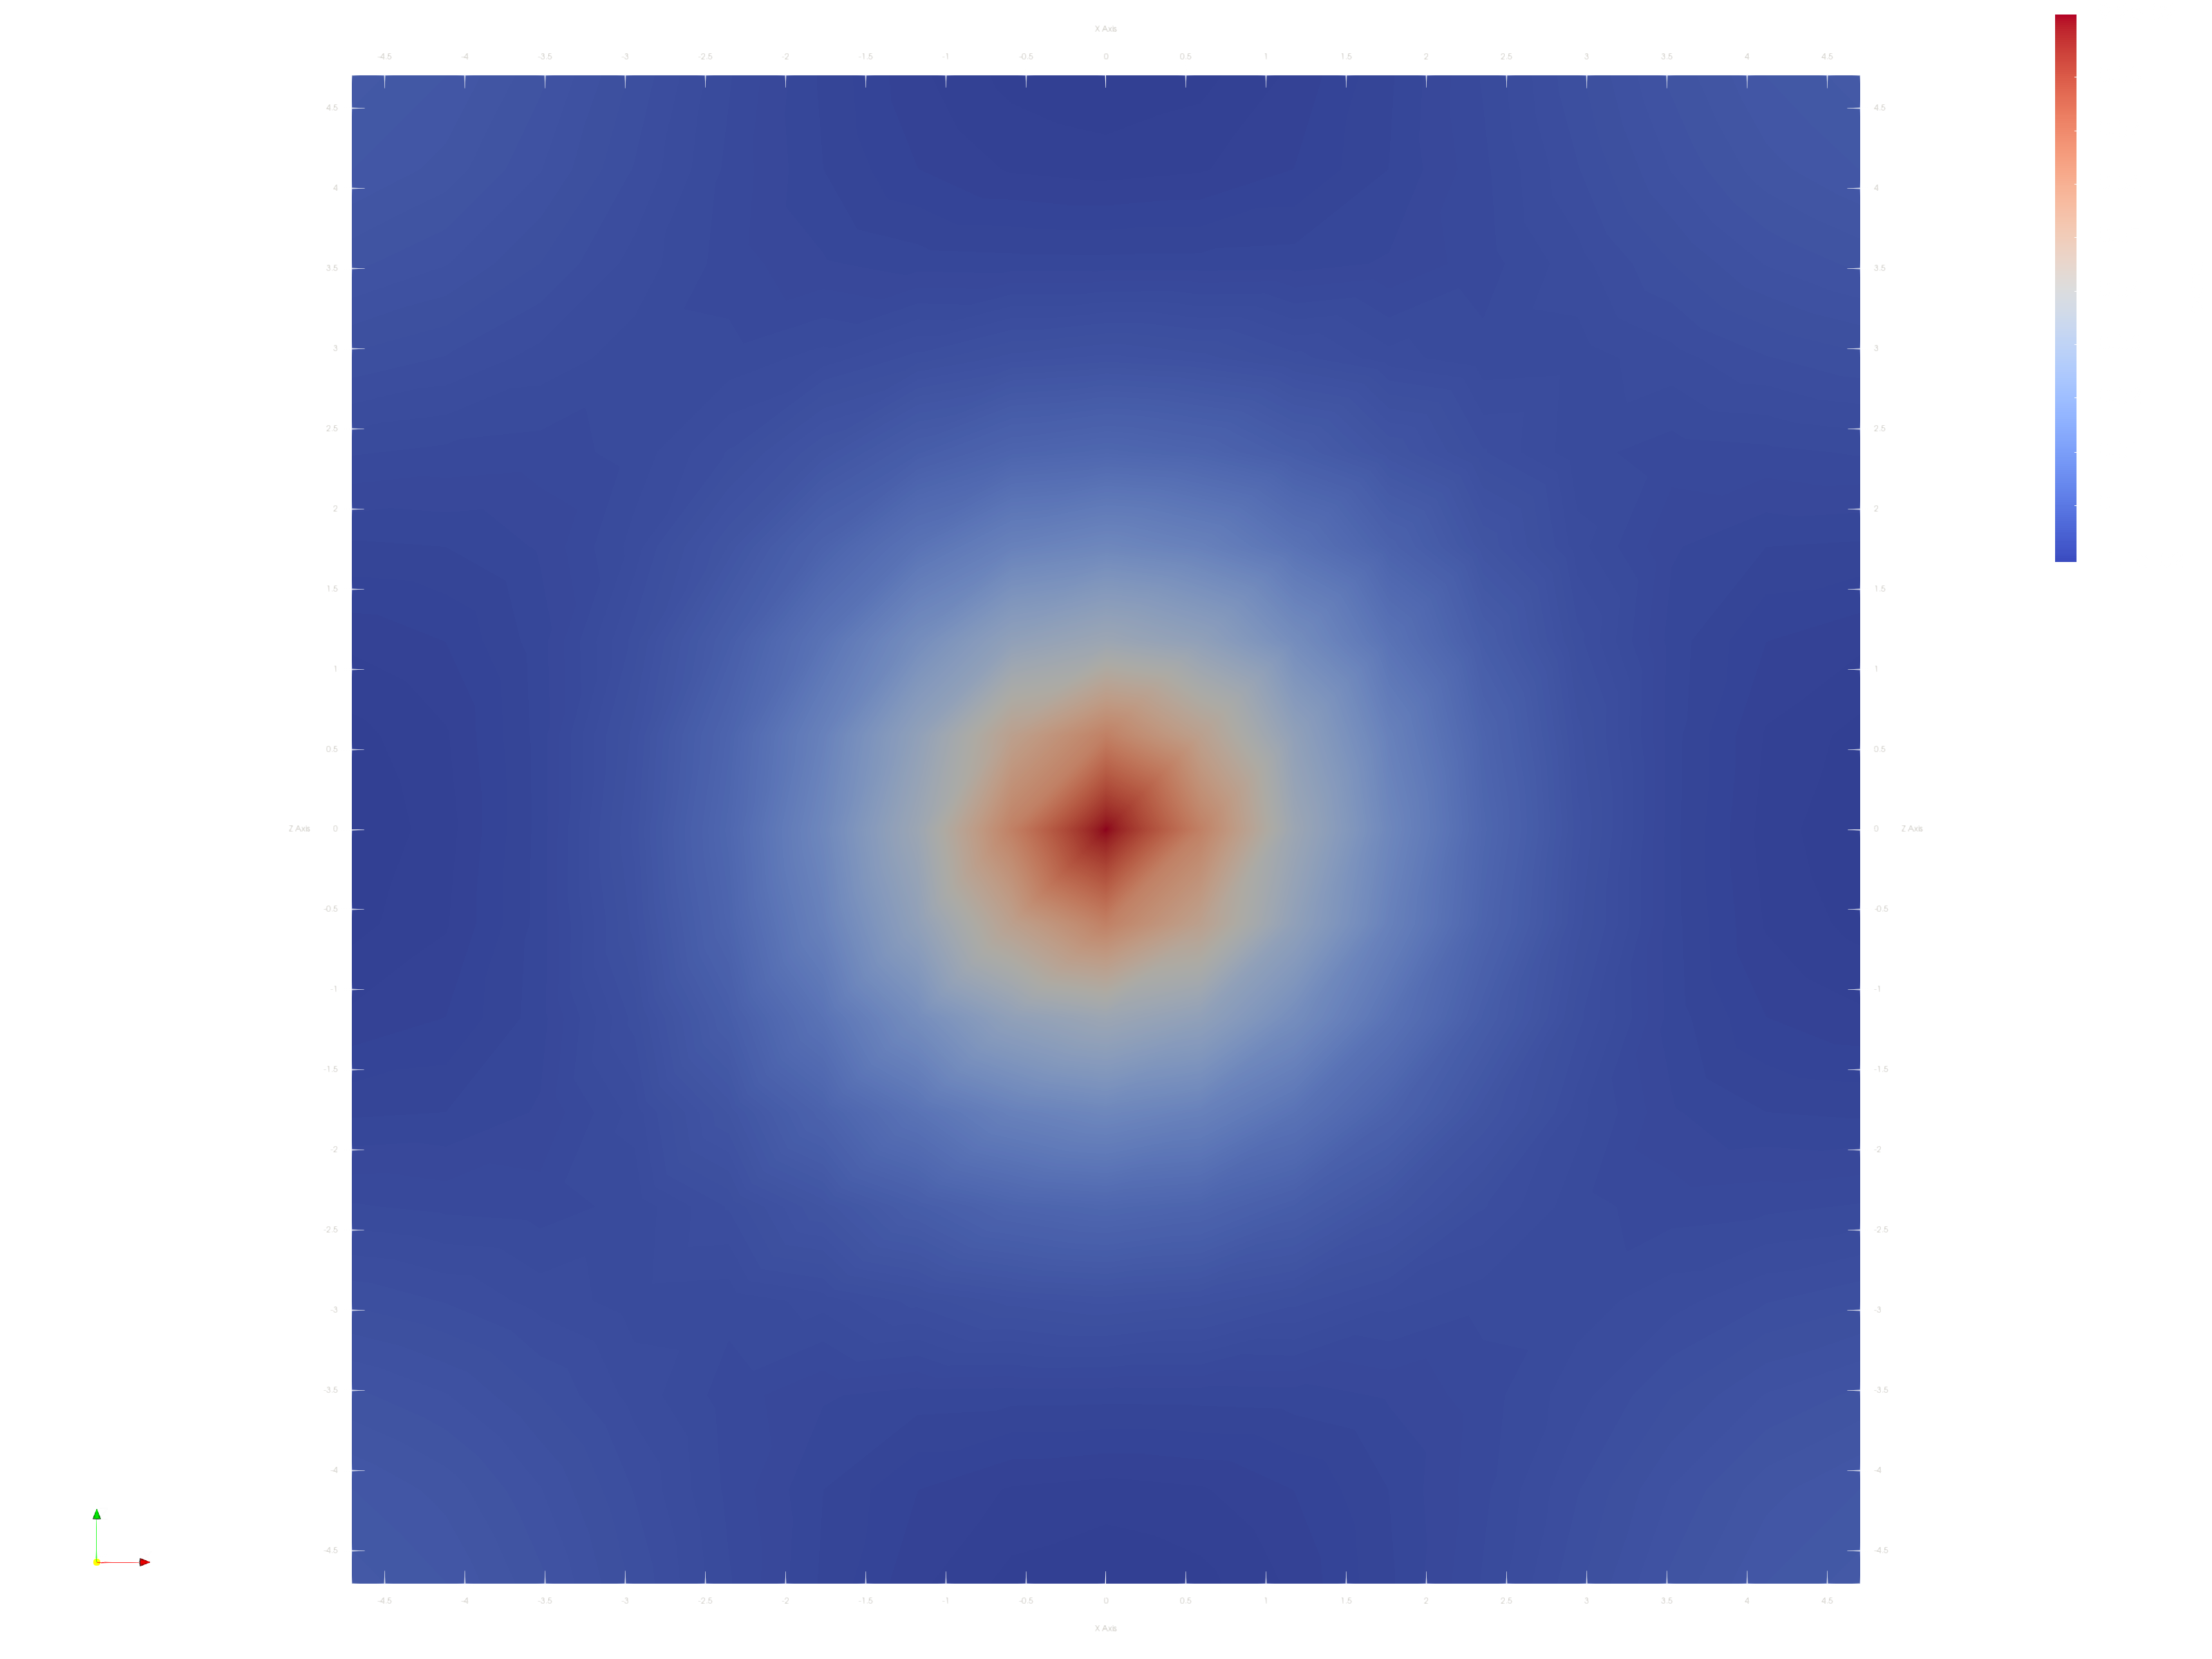
\includegraphics[width=0.32\linewidth]{images/kriging/3components/exact_cov_22_yy.png}}
        \hfill
        \subcaptionbox{$R_{yy}$ $z$-нормаль \label{img:kriging_exact_cov_r_33}} 
        {\includegraphics[width=0.32\linewidth]{images/kriging/3components/exact_cov_22_zz.png}}
        \hfill
        
        \subcaptionbox{$R_{zz}$ $x$-нормаль \label{img:kriging_exact_cov_r_22}} 
        {\includegraphics[width=0.32\linewidth]{images/kriging/3components/exact_cov_33_xx.png}}
        \hfill
        \subcaptionbox{$R_{zz}$ $y$-нормаль \label{img:kriging_exact_cov_r_23}} 
        {\includegraphics[width=0.32\linewidth]{images/kriging/3components/exact_cov_33_yy.png}}
        \hfill
        \subcaptionbox{$R_{zz}$ $z$-нормаль \label{img:kriging_exact_cov_r_33}} 
        {\includegraphics[width=0.32\linewidth]{images/kriging/3components/exact_cov_33_zz.png}}
        \hfill
    }
    
    \onehalfspacing{}
    \caption{Ковариационные функции, заданные для применения трёхмерного стохастического метода}
    \label{img:exact_covariance_comparison_heat_maps}  
\end{figure}

Первое, что необходимо заметить, это пространственное вытягивание компонент тензора в смежных плоскостях, в плоскостях, нормальных к текущей компоненте наблюдается симметрия ковариационной функции. При сравнении с численно полученным результатом также учтём это. Вне диагональные компоненты не представлены, так как их значение можно считать нулевыми.

Ниже представлены графики пространственной ковариации рассчитанные на 10000 реализаций полей флуктуаций полученные в результате трёхмерного стохастического моделирования. На рисунках представлены значения вдоль диагонали куба от точки $\{-5, -5, -5\}$ до точки $\{ 5, 5, 5 \}$ и значения вдоль осей координат.

%
% Ковариация по осям координат
%
\begin{figure}[ht] 
  \center
  \includegraphics [width=0.8\linewidth] {images/kriging/3components/calculated_all_diag.png}
  \caption{Расчётная ковариационная функция $R_{ik}$ на основе стохастического метода вдоль диагонали области } 
  \label{img:kriging_covariances_diag}  
\end{figure}

\begin{figure}[ht] 
  \center
  \includegraphics [width=0.8\linewidth] {images/kriging/3components/calculated_all_x.png}
  \caption{Расчётная ковариационная функция $R_{ik}$ на основе стохастического метода вдоль оси $x$ области } 
  \label{img:kriging_covariances_diag}  
\end{figure}

\begin{figure}[ht] 
  \center
  \includegraphics [width=0.8\linewidth] {images/kriging/3components/calculated_all_y.png}
  \caption{Расчётная ковариационная функция $R_{ik}$ на основе стохастического метода вдоль оси $y$ области } 
  \label{img:kriging_covariances_diag}  
\end{figure}

\begin{figure}[ht] 
  \center
  \includegraphics [width=0.8\linewidth] {images/kriging/3components/calculated_all_z.png}
  \caption{Расчётная ковариационная функция $R_{ik}$ на основе стохастического метода вдоль оси $z$ области } 
  \label{img:kriging_covariances_diag}  
\end{figure}

Как можно видеть из приведённых выше графиков, наблюдается вытягивание вдоль соответствующих компонент. Также наблюдается достаточно высокая визуальная симметрия относительно начала координат. С ростом расстояния наблюдаются большие отклонения ковариационной функции, связанные с тем, что выборка, на которой рассчитывались ковариационные функции конечна. Ниже представлены сравнения полученных ковариационны функций для диагональных компонент в различных направлениях с задаваемыми, а также с симметризованной относительно начала координат расчётной ковариационной функцией.

\begin{figure}[ht] 
  \center
  \includegraphics [width=0.8\linewidth] {images/kriging/3components/diagonal_r11_x.png}
  \caption{Расчётная ковариационная функция $R_{xx}$ на основе стохастического метода вдоль диагонали области } 
  \label{img:kriging_covariances_diag}  
\end{figure}

\begin{figure}[ht] 
  \center
  \includegraphics [width=0.8\linewidth] {images/kriging/3components/diagonal_r22_yy.png}
  \caption{Расчётная ковариационная функция $R_{yy}$ на основе стохастического метода вдоль диагонали области } 
  \label{img:kriging_covariances_diag}  
\end{figure}

\begin{figure}[ht] 
  \center
  \includegraphics [width=0.8\linewidth] {images/kriging/3components/diagonal_r33_zz.png}
  \caption{Расчётная ковариационная функция $R_{zz}$ на основе стохастического метода вдоль диагонали области } 
  \label{img:kriging_covariances_diag}  
\end{figure}

По правой части графиков можно заметить насколько расчётная ковариационная функция не симметрична. Из-за этого дальнейшие расчёты тензора спектра скоростей и энергетического спектра проводились на симметризованной ковариационной функции. Процедура симметризации спектра необходима для устранения фазового смещения будущего тензора спектра скоростей, так как в ином случае при проведении преобразования Фурье, возникает мнимая часть, связанная с фазовым сдвигом, возникающим в следствии несимметричности функции, так как использовалось быстрое преобразование Фурье, требующее искусственного продолжения периодического сигнала. Возникающий скачок между продолженными ковариационными функциями, вносит фазовое смещение, откуда и возникает мнимая часть преобразования. Можно сказать, что мы рассматриваем не весь куб, а лишь его первый октант, данные для которого были симметрично продолжены относительно начала координат и граничащих плоскостей координат. 

Из-за мало корреляции компонент скоростей на больших расстояниях, также присутствуют большие отклонения ковариационной функции относительно задаваемой, что также вносит свою небольшую ошибку. Этот эффект отражается на последующем преобразовании Фурье при переходе от функций пространственной ковариации к тензору спектра скоростей. Ниже представлено сравнение расчётных значений тензора спектра скоростей с полученными применением формулы \eqref{eq:part3_2}. 
\noindent
\begin{figure}[!h]
    \center{
        \hfill
        \subcaptionbox[List-of-Figures entry]{$R_{xx}$\label{img:kriging_computed_phi_11_diagonal}} 
        {\includegraphics[width=0.34\linewidth]{images/kriging/3components/phi_11_diagonal.png}}%
        \hfill       
        \subcaptionbox{$R_{xy}$ и $R_{yx}$\label{img:kriging_computed_phi_12_diagonal}} 
        {\includegraphics[width=0.34\linewidth]{images/kriging/3components/phi_12_21_diagonal.png}} \\
        \hfill
        \subcaptionbox{$R_{xz}$ и $R_{zx}$\label{img:kriging_computed_phi_13_diagonal}} 
        {\includegraphics[width=0.34\linewidth]{images/kriging/3components/phi_13_31_diagonal.png}}
        \hfill       
        \subcaptionbox{$R_{yy}$\label{img:kriging_computed_phi_22_diagonal}} 
        {\includegraphics[width=0.34\linewidth]{images/kriging/3components/phi_22_diagonal.png}} \\
        \hfill
        \subcaptionbox{$R_{yz}$ и $R_{yz}$\label{img:kriging_computed_phi_23_diagonal}} 
        {\includegraphics[width=0.34\linewidth]{images/kriging/3components/phi_23_32_diagonal.png}}
        \hfill
        \subcaptionbox{$R_{zz}$\label{img:kriging_computed_phi_33_diagonal}} 
        {\includegraphics[width=0.34\linewidth]{images/kriging/3components/phi_33_diagonal.png}}
        \hfill
    }
    
    \onehalfspacing{Функции тензора спектра энергий представлены дволь диагонали куба в пространстве фурье $n=17$, $k_l=10$}
    \caption{Ковариационные функции, заданные для применения трёхмерного стохастического метода}
    \label{img:exact_covariance_comparison_heat_maps}  
\end{figure}

Как можно заметить, основные различия между вычисленными и заданными компонентами тензора присутствуют при $\Phi \approx 0$. Далее используя формулу \eqref{eq:part3_2} перейдём от тензора спектра скоростей к энергетическому спектру. 

\begin{figure}[ht] 
  \center
  \includegraphics [width=0.9\linewidth] {images/kriging/3components/energy_function_kriging_loglog.png}
  \caption{Энергетический спектр поля скоростей полученный в результате стохастического моделирования в сравнении с целевым спектром в логарифмических координатах} 
  \label{img:kriging_spectra_function_compare}  
\end{figure}

Полученный спектр хорошо сходится с целевым спектров области наиболее энергонесущих мод. Есть сходство со спектром получаемым в результате метода Крайшнана, в частности резкое убывание, предположительно связанное с критерием Нейквиста.

Рассмотрим генерацию поля флуктуаций с использованием последовательного моделирования. Как говорилось в \ref{chapt1}, в данном случае, основным параметров генерации, который мы можем варьировать -- число ближайших соседей, учитываемых при расчёта среднего и ковариации величины в точке. Наиболее оптимальным оказалось число $N=15$ при котором наблюдается хорошая аппроксимация целевого спектра, а также достаточно высокая производительность. Для обычного непоследовательного стохастического метода, помимо высокого затрачиваемого процессорного времени, требуется достаточно большой объём памяти, что может сильно ограничить возможность генерации на подробных сетках. В свою очередь, метод последованных симуляций позволяет сократить требуемое количество памяти, за счёт отказа от хранения матрицы ковариаций целиком (теперь необходимо хранить матрицы $n \times n$). Малое число параметров, позволяет более простым образом задать требуемый спектр. Ниже представлено сравнение спектров, результирующего, полученного с использованием 1000 реализаций поля генерируемого последовательным методом. Параметры сеток задавилсь следующими: для сетки пространства Фурье $l_F=20$, $n_F = 51$, для сетки физического пространства $n_{P} = 31$, $l=10$. Число учитываемых ближайших соседей $N = 15$.

\begin{figure}[ht] 
    \center
    \includegraphics [width=0.8\linewidth] {images/kriging/spectrum.png}
    \caption{Сравнение энергетического спектра для предлагаемой модиификации спектрального метода с целевым} 
    \label{img:kriging_result_field_no_angle}  
\end{figure}

\begin{figure}[ht] 
    \center
    \includegraphics [width=0.8\linewidth] {images/kriging/spectrum_loglog.png}
    \caption{Сравнение энергетического спектра для предлагаемой модиификации спектрального метода с целевым в логарифмических координатах} 
    \label{img:kriging_result_field_on_angle}  
\end{figure}

Как и в случае спектрального метода, наблюдается разница в спектрах для малых волновых чисел, в остальном, особенно в инерционном интервале, получаем практически точное сходство. Наибольшое отклонение результирующего от задаваемого спектров $\Delta E = 0.025$, но также стоит отметить, что это значение находится в волнвых числах меньше чем минимальное волнове число на сетке $k_{min}=\frac{2 \pi}{10} \approx 0.628$. Как было сказано выше основным критерием выбора метода является удовлетворению целевому спектру. Рассмотрим сравнение полученных спектров обоими методами с целевым спектром.

\begin{figure}[ht] 
    \center
    \includegraphics [width=0.8\linewidth] {images/comparison_of_result_spectras.png}
    \caption{Сравнение энергетического спектра для предлагаемой модиификации спектрального метода с целевым в логарифмических координатах} 
    \label{img:main_comparison_of_target_spectras}  
\end{figure}

Для полей получаемых по результатам спектрального метода, наблюдается лучшая точность при малых волновых числах, с учётом того что существуют ограничения на волновые числа многократно описанные выше. Метод последовательных симуляций лучшим образом аппроксиммирует спектр в инерционном интервале, а также имеет более точное совпадение пика для наиболее энергонесущей волны. Но по сравнению со спектральным методом, данный имеет большее затрачиваемое время на одну реализацию. С сетки и параметра $N$ описанных выше, генерация 1000 полей происходит за 2 минуты 14 секунд, одна реализация требует $\frac{134}{1000} \approx 0.134$ секунд, без учёта времени на запись результатов, результат больше чем требуется для спектрального метода в 3 раза.